% Options for packages loaded elsewhere
\PassOptionsToPackage{unicode}{hyperref}
\PassOptionsToPackage{hyphens}{url}
%
\documentclass[
  openany]{book}
\usepackage{amsmath,amssymb}
\usepackage{iftex}
\ifPDFTeX
  \usepackage[T1]{fontenc}
  \usepackage[utf8]{inputenc}
  \usepackage{textcomp} % provide euro and other symbols
\else % if luatex or xetex
  \usepackage{unicode-math} % this also loads fontspec
  \defaultfontfeatures{Scale=MatchLowercase}
  \defaultfontfeatures[\rmfamily]{Ligatures=TeX,Scale=1}
\fi
\usepackage{lmodern}
\ifPDFTeX\else
  % xetex/luatex font selection
\fi
% Use upquote if available, for straight quotes in verbatim environments
\IfFileExists{upquote.sty}{\usepackage{upquote}}{}
\IfFileExists{microtype.sty}{% use microtype if available
  \usepackage[]{microtype}
  \UseMicrotypeSet[protrusion]{basicmath} % disable protrusion for tt fonts
}{}
\makeatletter
\@ifundefined{KOMAClassName}{% if non-KOMA class
  \IfFileExists{parskip.sty}{%
    \usepackage{parskip}
  }{% else
    \setlength{\parindent}{0pt}
    \setlength{\parskip}{6pt plus 2pt minus 1pt}}
}{% if KOMA class
  \KOMAoptions{parskip=half}}
\makeatother
\usepackage{xcolor}
\usepackage{longtable,booktabs,array}
\usepackage{calc} % for calculating minipage widths
% Correct order of tables after \paragraph or \subparagraph
\usepackage{etoolbox}
\makeatletter
\patchcmd\longtable{\par}{\if@noskipsec\mbox{}\fi\par}{}{}
\makeatother
% Allow footnotes in longtable head/foot
\IfFileExists{footnotehyper.sty}{\usepackage{footnotehyper}}{\usepackage{footnote}}
\makesavenoteenv{longtable}
\usepackage{graphicx}
\makeatletter
\def\maxwidth{\ifdim\Gin@nat@width>\linewidth\linewidth\else\Gin@nat@width\fi}
\def\maxheight{\ifdim\Gin@nat@height>\textheight\textheight\else\Gin@nat@height\fi}
\makeatother
% Scale images if necessary, so that they will not overflow the page
% margins by default, and it is still possible to overwrite the defaults
% using explicit options in \includegraphics[width, height, ...]{}
\setkeys{Gin}{width=\maxwidth,height=\maxheight,keepaspectratio}
% Set default figure placement to htbp
\makeatletter
\def\fps@figure{htbp}
\makeatother
\setlength{\emergencystretch}{3em} % prevent overfull lines
\providecommand{\tightlist}{%
  \setlength{\itemsep}{0pt}\setlength{\parskip}{0pt}}
\setcounter{secnumdepth}{5}
%%%
%\usepackage[a4paper, total={6in, 8.6in}]{geometry}
\usepackage[a4paper, total={125mm, 200mm}]{geometry}
%%
\usepackage{polyglossia}  \setdefaultlanguage{polish}
%%
\usepackage{booktabs}
\usepackage{fontspec}
%\defaultfontfeatures{Mapping=TeX}
\setmainfont[Ligatures=TeX]{Cambria}
%\setmainfont{Cambria}
\setmathfont{Cambria Math}
%% Supress any other theorems (probably)
\newtheorem{theorem}{}
%%
%% This is not working
%% https://github.com/jgm/pandoc/issues/4384
%%
\makeatletter
\def\maxwidth{\ifdim\Gin@nat@width>\linewidth\linewidth\else\Gin@nat@width\fi}
\def\maxheight{\ifdim\Gin@nat@height>\textheight\textheight\else\Gin@nat@height\fi}
\renewcommand\section{\@startsection {section}{1}{\z@}%
                                   {-3.5ex \@plus -1ex \@minus -.2ex}%
                                   {2.3ex \@plus.2ex}%
                                   {\raggedright \normalfont\Large\bfseries}}
\renewcommand\subsection{\@startsection{subsection}{2}{\z@}%
                                     {-3.25ex\@plus -1ex \@minus -.2ex}%
                                     {1.5ex \@plus .2ex}%
                                     {\raggedright \normalfont\large\bfseries}}

\def\@makechapterhead#1{%
  %%\vspace*{50\p@}%
  {\parindent \z@ \raggedright \normalfont
    \ifnum \c@secnumdepth >\m@ne
      \if@mainmatter
        \large\bfseries \@chapapp\space \thechapter
        \par\nobreak
        %\vskip 5\p@
        %\medskip
      \fi
    \fi
    \interlinepenalty\@M
    \LARGE \bfseries #1\par\nobreak
    \vskip 20\p@
  }}
\def\@schapter#1{\if@twocolumn
                   \@topnewpage[\@makeschapterhead{#1}]%
                 \else
                   \@makeschapterhead{#1}%
                   \@afterheading
                 \fi}
\def\@makeschapterhead#1{%
  %%\vspace*{50\p@}%
  {\parindent \z@ \raggedright
    \normalfont
    \interlinepenalty\@M
    \huge \bfseries  #1\par\nobreak
    \vskip 20\p@
  }}

%%%
\renewcommand\tableofcontents{%
    \if@twocolumn
      \@restonecoltrue\onecolumn
    \else
      \@restonecolfalse
    \fi
    \chapter*{\contentsname
        \@mkboth{\contentsname}{\contentsname}}%
    \@starttoc{toc}%
    \if@restonecol\twocolumn\fi
    }
%% default latex figure options
\renewcommand*{\fps@figure}{!htb}
\setlength\parskip{0\p@ \@plus \p@}
\setlength\parindent{15\p@}
%%
%% Already defined
\RequirePackage{etoolbox}
%%%\preto{\@verbatim}{\topsep=3pt \partopsep=3pt }
\AtBeginEnvironment{tabular}{\medskip}
\AfterEndEnvironment{tabular}{\par\medskip}
%%
\AtBeginEnvironment{verbatim}{\medskip}
\AfterEndEnvironment{verbatim}{\par\medskip}
%%
%%
%%
\makeatother
%%%
\AtBeginDocument{%%
 \let\maketitle\relax
  %% Insert title page
 \begin{titlepage}
 \begingroup  
 %% reset
 \setkeys{Gin}{width=210mm,height=300mm}
\vbox to \textheight{\vss%
   \hbox to\textwidth{\hss
     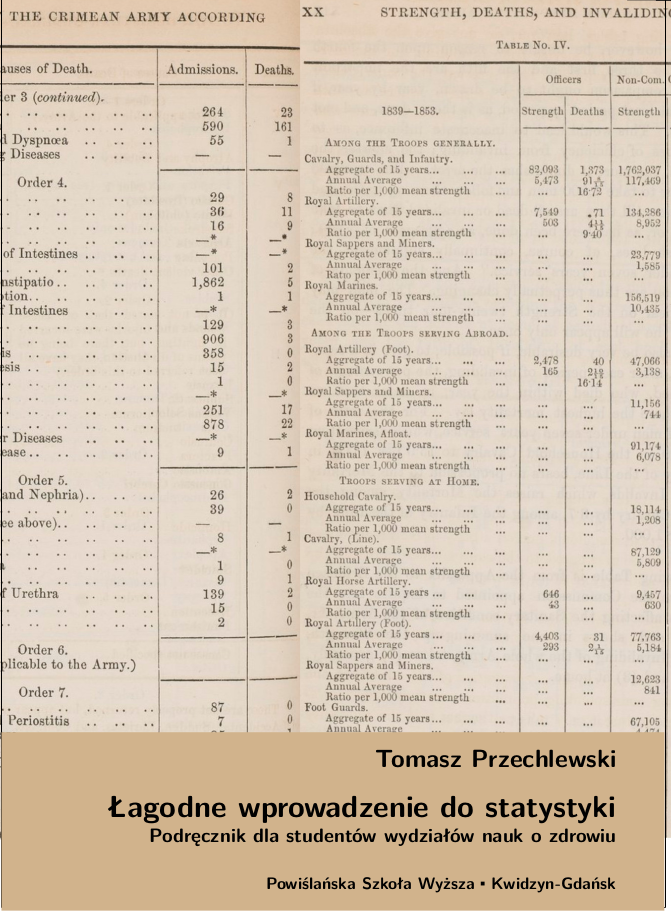
\includegraphics[width=210mm]{Cover_03.png}\hss}
   \vss}
\vbox to \textheight{%
  \vskip20mm
  \noindent
   Na okładce: Statystyki zdrowia armii brytyjskiej z okresu wojny krymskiej\\
   Notes on matters affecting the health, efficiency,\\
   and hospital administration of the British Army\\
   by Nightingale, Florence, 1820-1910\\
   \url{https://archive.org/details/b20387118/}
   \vskip20mm
   \noindent
   Książka została zredagowana w formacie Rmarkdown/bookdown
.

   \vskip20mm
   \noindent
   Kolorowa wersja podręcznika znajduje się pod adresem:\\
   \url{https://hrpunio.github.io/SMI_Bookdown/wstęp.html}

   \vskip20mm
   \noindent
   Recenzent: Michał Pietrzak
  \vss
}
\endgroup
\end{titlepage}
\author{Tomasz Przechlewski\\ Powiślańska Szkoła Wyższa\\(Kwidzyn-Gdańsk)}%
}

\usepackage[most]{tcolorbox}
\newtcolorbox{TPexample}[1][]{%
    colback=white,
    colframe=blue!50!black,
    %%boxsep=0pt,
    left=3pt,right=3pt, top=2pt, bottom=2pt,
    notitle,
    %%sharp corners,
    enhanced,
    breakable,
}
\newenvironment{example}{\begin{TPexample}%
\setlength{\abovedisplayskip}{0pt plus 3pt}%
\parskip1ex}{\end{TPexample}}


\font\chineseFont="NotoSansTC-Regular" at 10pt
\def\chinese#1{{\chineseFont #1}}
\edef\bbChar{□}
\edef\bbCharX{☒}
\edef\bbArrowR{→}

\catcode`☒=\active
\catcode`□=\active
\catcode`→=\active
\def☒{\chinese{\bbCharX}} %% bb with X
\def□{\chinese{\bbChar}} %% ballot box
\def→{\chinese{\bbArrowR}} %% right arrow

%%\newenvironment{tof}{\begingroup\medskip }{\par\medskip\endgroup}

%%\setlength{\abovedisplayskip}{0pt plus 6pt}
%%\setlength{\belowdisplayskip}{1em}
%%\setlength{\abovedisplayshortskip}{0em}


%%% Redefine headers
\renewcommand{\chaptermark}[1]{ \markboth{#1}{} }
\renewcommand{\sectionmark}[1]{ \markright{#1}{} }
%%% Excessive skip
\setlength{\abovedisplayskip}{6pt plus 6pt}
\setlength{\belowdisplayskip}{6pt plus 6pt}
\setlength{\abovedisplayshortskip}{0pt plus 3pt}
\setlength{\belowdisplayshortskip}{0pt plus 3pt}
\parindent12pt
\parskip0pt
%%% end-of-preamble
\ifLuaTeX
  \usepackage{selnolig}  % disable illegal ligatures
\fi
\usepackage[]{natbib}
\bibliographystyle{plainnat}
\IfFileExists{bookmark.sty}{\usepackage{bookmark}}{\usepackage{hyperref}}
\IfFileExists{xurl.sty}{\usepackage{xurl}}{} % add URL line breaks if available
\urlstyle{same}
\hypersetup{
  pdftitle={Podstawy statystyki},
  hidelinks,
  pdfcreator={LaTeX via pandoc}}

\title{Podstawy statystyki}
\usepackage{etoolbox}
\makeatletter
\providecommand{\subtitle}[1]{% add subtitle to \maketitle
  \apptocmd{\@title}{\par {\large #1 \par}}{}{}
}
\makeatother
\subtitle{Podręcznik dla studentów wydziałów nauk o zdrowiu}
\author{true}
\date{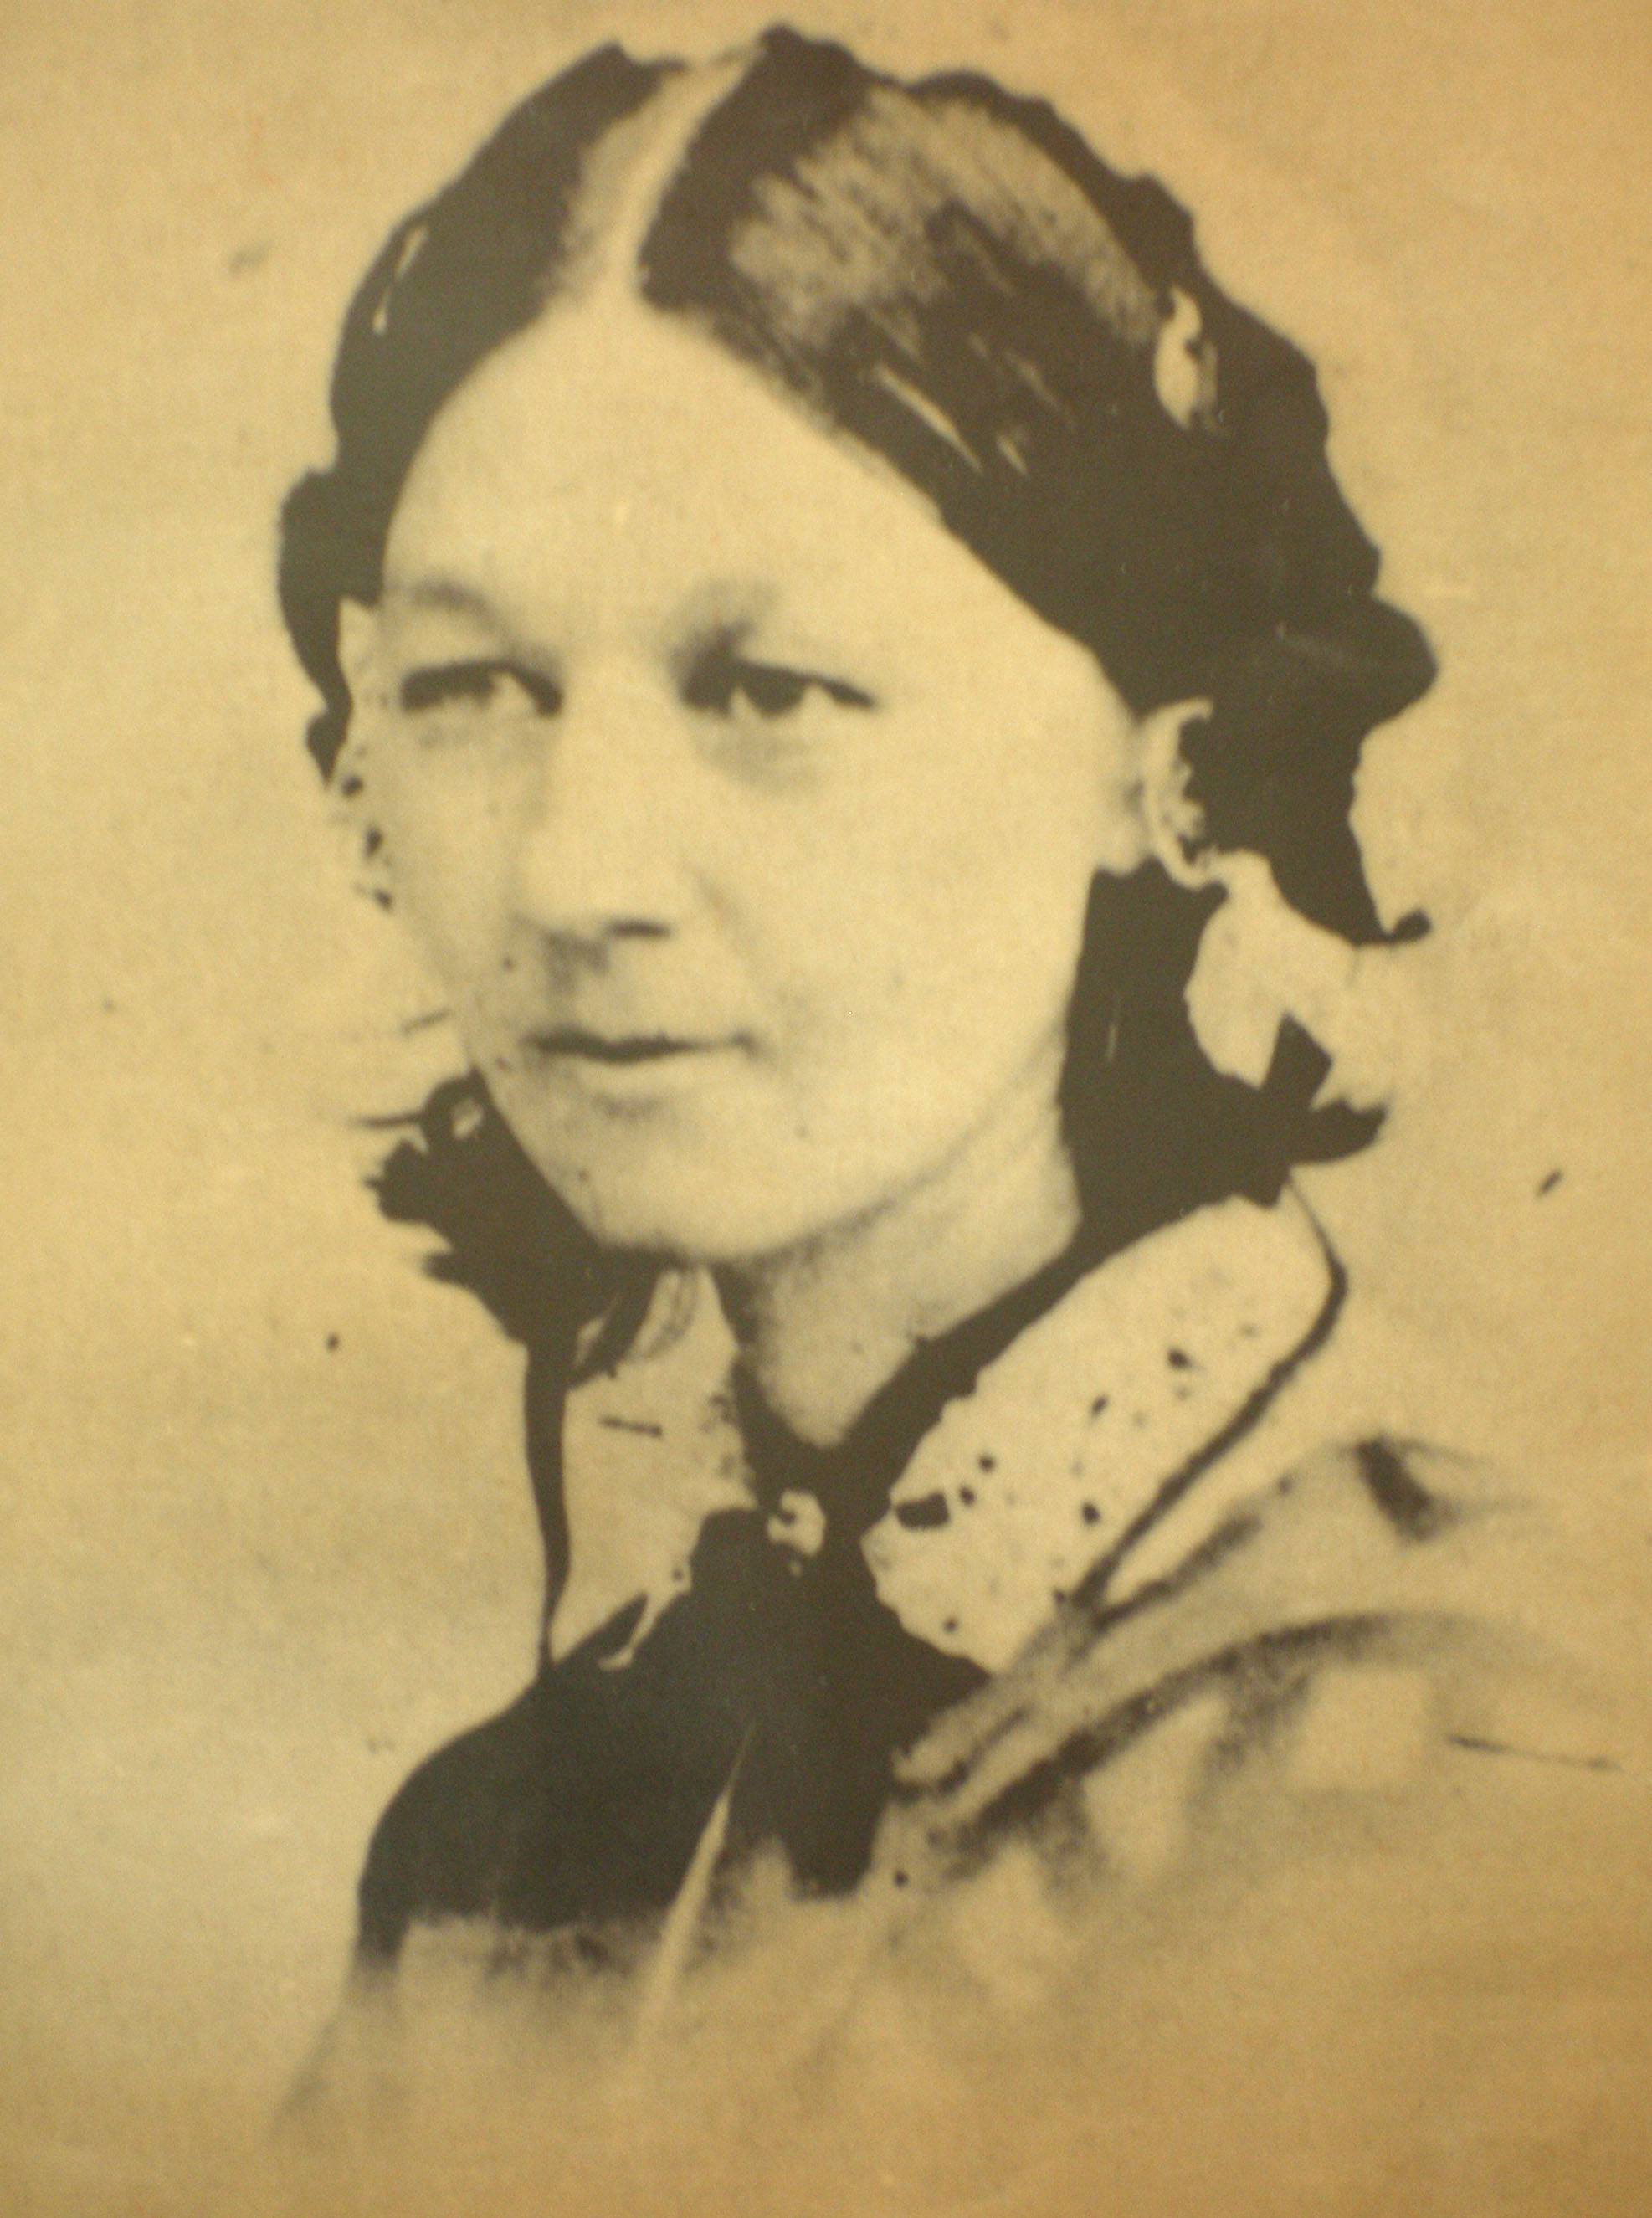
\includegraphics[width=0.5\textwidth,height=\textheight]{./FN.jpg}}

\begin{document}
\maketitle

{
\setcounter{tocdepth}{1}
\tableofcontents
}
\hypertarget{wstux119p}{%
\chapter*{Wstęp}\label{wstux119p}}
\addcontentsline{toc}{chapter}{Wstęp}

Przygotowując się kilka lat temu do zajęć z przedmiotu Statystyka Medyczna
ze zdumieniem odkryłem, że
nie istnieje coś takiego jak polski podręcznik do statystyki medycznej
powszechnie dostępny w księgarni, który mogę polecić
swoim studentom. Byłem tym tym bardziej zdziwiony, że wiedziałem już wtedy
co oznacza akronim EBM.
W tamtym czasie prawdę mówiąc była tylko jedna
książka ze statystyką medyczną w tytule -- absolutnie moim zdaniem
nie nadająca się do polecenia jej komukolwiek kto chciałby się
nauczyć statystyki.
Jest to książka tak \textbf{beznadziejna}, że nie wymienię nawet jej tytułu --
tłumaczenie
z języka angielskiego zresztą.

W trakcie zajęć odkryłem także, że studenci w ogromnej większości
są przekonani, że przedmiot ten jest trudny i mają w związku z tym
ogromną -- graniczącą z pewnością -- obawę, że nie są w stanie go opanować.

W moim przekonaniu żeby ten stan rzeczy zmienić należy zademonstrować
-- teoretycznie oraz praktycznie -- że statystyka nie jest
wcale aż taka trudna. Teoretycznie oznaczałoby,
że cześć matematyczna powinna być zredukowana do absolutnego minimum,
a praktycznie, że należy pokazać jak i czym da się łatwo statystkę uprawiać
czyli liczyć. Przez \textbf{czym} oczywiście współcześnie należy
rozumieć konkretny program komputerowy i niekoniecznie tym programem musi być
arkusz kalkulacyjny.

Sposobem na lepsze zrozumienie statystyki nie może być zasypanie
studenta wielopiętrowymi formułami matematycznymi (co dyskwalifikuje
część podręczników), ale raczej zastąpienie formalnej ścisłości
przykładami i odwołanie się do zdrowego rozsądku, który przecież
jest istotą wielu procedur statystycznych, takich jak na przykład
testy istotności.

Kierując się tym założeniem całość teorii wyłożono w czterech pierwszych
rozdziałach podręcznika.
W pierwszym jak to zwykle bywa przedstawiono czym jest statystyka,
czym się zajmuje oraz wyjaśniono \textbf{podstawowe pojęcia}, którymi
statystyka się posługuje, takie jak populacja, próba czy pomiar.
W rozdziale drugim przedstawiono metody \textbf{opisu statystycznego}.
Rozdział trzeci przedstawia ideę \textbf{wnioskowania statystycznego}.
Najbardziej
obszerny rozdział czwarty opisuje metody \textbf{analizy zależności}.

Pozostałe rozdziały poświęcono praktyce. Rozdział piąty zawiera
przykładowe analizy trzech badań ankietowych a rozdział szósty
opisuje
jak uprawiać statystykę z wykorzystaniem programu Jamovi.

Podręcznik został napisany dla studentów Wydziału Nauk o Zdrowiu
Powiślańskiej Szkoły Wyższej, których uczę od kilku lat
statystyki medycznej, ale mam nadzieję że może być przydatny
także dla studentów innych kierunków zwłaszcza kierunków medycznych.

Elektroniczne wersje podręcznika w formatach HTML, PDF oraz EPUB znajdują
się pod adresem:
\href{https://hrpunio.github.io/SMI_Bookdown/wstęp.html}{hrpunio.github.io/SMI\_Bookdown/wstęp.html}.
Wykorzystane
w omawianych w książce przykładach zbiory danych można znaleźć
pod adresem: \href{https://github.com/hrpunio/SMBook}{github.com/hrpunio/SMBook}.

\hypertarget{przedmiotbadan}{%
\chapter{Przedmiot i metody badań statystycznych}\label{przedmiotbadan}}

\hypertarget{przedmiotS}{%
\section{Przedmiot statystyki}\label{przedmiotS}}

Wyraz statystyka ma wiele znaczeń: \textbf{statystyki zgonów} albo \textbf{statystyki
alkoholizmu} czyli \textbf{dane} dotyczące zgonów lub alkoholizmu.
Statystyka to też \textbf{dziedzina wiedzy}, upraszczając zbiór metod, które służą
do tworzenia statystyk w pierwszym znaczeniu tego słowa.
Wreszcie statystyka to \textbf{pojedyncza metoda} ze zbioru metod opracowanych
w dziedzinie, np. średnia to statystyka. Trochę to niefortunne, ale
świat nie jest doskonały jak wiemy.

\textbf{Statystyka} (obiegowo): dział matematyki, a w związku z tym
wiedza absolutnie
pewna i obiektywna. Nieprawda choćby z tego powodu,
że nie jest działem matematyki.
Korzysta z metod matematycznych jak wiele innych dziedzin.

\textbf{Statystyka} od strony czysto praktycznej to: \textbf{dane} + \textbf{procedury}
(zbierania, przechowania, analizowania, prezentowania \emph{danych})
+ \textbf{programy}; Jeżeli statystyka kojarzy się komuś ze matematyką,
wzorami i liczeniem, to jak widać jest to zaledwie podpunkt
procedury→analizowanie.

\hypertarget{podstawowe-pojux119cia}{%
\section{Podstawowe pojęcia}\label{podstawowe-pojux119cia}}

Celem \textbf{badania statystycznego} jest uzyskanie informacji
o interesującym zjawisku na podstawie danych.
Zjawisko ma charakter masowy czyli dotyczy dużej liczby \emph{obiektów}.
Nie interesuje nas jeden zgon (obiekt) tylko zgony wielu ludzi.

\textbf{Populacja} (\textbf{zbiorowość statystyczna}) to zbiór obiektów będący
przedmiotem badania statystycznego. Na przykład zgony w Polsce w roku 2022.

Każdy \textbf{obiekt} w populacji to
\textbf{obserwacja} (zwana także \textbf{jednostką statystyczną} albo \textbf{pomiarem})
na jednej lub więcej \textbf{zmiennych} (albo \textbf{cech}).
Jeżeli interesującym zjawiskiem są zgony, obserwacją jest osoba zmarła
a zmiennymi (cechami) wiek,
płeć, przyczyna zgonu oraz dzień tygodnia (w którym nastąpił zgon) zmarłej osoby.

\textbf{Próba} to część \textbf{populacji}.
Na przykład część zgonów w Polsce w roku 2022.

\textbf{Parametr}: wielkość numeryczna obliczona na podstawie populacji.

\textbf{Statystyka}: wielkość numeryczna obliczona na podstawie próby.

Populacja powinna być zdefiniowana w taki sposób, aby nie było wątpliwości
co tak naprawdę jest badane. Zgony to w oczywisty sposób za mało.
\emph{Zgony mieszkańców Kwidzyna w roku 2022}.

Zwróćmy uwagę, że \emph{Zgony w mieście Kwidzyn w roku 2022} to nie to samo
(ktoś może być mieszkańcem
a umrzeć w Polsce i/lub ktoś może nie być mieszkańcem i umrzeć w Kwidzynie).

\textbf{Generalizacja}: ocena całości na podstawie części. Badamy zjawisko wypalenia
zawodowego pielęgniarek i pielęgniarzy w Polsce (populacja). Wobec zaporowych kosztów
mierzenia wszystkich decydujemy się na przeprowadzenie ankiety wśród studentów
pielęgniarstwa PSW (próba). Czy możemy twierdzić na podstawie próby, że wyniki
badania dla całej Polski są identyczne? Raczej nie.

Próba, która pozwala na generalizację nazywa się próbą \textbf{reprezentatywną}.
Najlepszym sposobem na uzyskanie próby reprezentatywnej jest losowanie.

W oczywisty sposób badanie na podstawie próby jest tańsze niż badanie całości, co nie
oznacza że jest tanie. Kontynuując przykład: musielibyśmy mieć listę wszystkich
pielęgniarek i pielęgniarzy w Polsce. Z tej listy wylosować próbę a następnie skontaktować
się z wybranymi osobami (jak?). Dlatego też badania w oparciu o próbę nielosową są całkiem
popularne (bo są tanie); należy jednakże mieć świadomość ich ograniczeń, w tym a zwłaszcza
uogólnienia uzyskanych wyników.

\hypertarget{pomiar}{%
\section{Pomiar}\label{pomiar}}

Potocznie kojarzy się z linijką i wagą, ale w statystyce używany jest w szerszym
znaczeniu. Ustalenie płci albo przyczyny zgonu to też pomiar.

\textbf{Pomiar} to przyporządkowanie wariantom \textbf{zmiennej} liczb lub symboli z pewnej \textbf{skali pomiarowej}.
Przykładowo jeżeli jednostką statystyczną jest zgon a zmiennymi
wiek, płeć,
przyczyna zgonu oraz dzień tygodnia to
pomiar będzie polegał na ustaleniu (przyporządkowaniu) wieku w latach,
płci (`K'/`M'), przyczyny (identyfikatora z katalogu ICD10 zapewne)
oraz numeru dnia tygodnia (lub nazwy dnia tygodnia).
Wiek oraz numer dnia są liczbami, płeć i przyczyna symbolem.

Wyróżnia się następujące \textbf{typy skal pomiarowych}:

\begin{itemize}
\item
  \textbf{nominalna} (\emph{nominal scale}), klasyfikuje: płeć zmarłego;
\item
  \textbf{porządkowa} (\emph{ordinal scale}), klasyfikuje i porządkuje: dzień tygodnia
  w którym nastąpił zgon (po poniedziałku jest wtorek);
\item
  \textbf{liczbowa}, mierzy w potocznym tego słowa znaczeniu: wiek zmarłego w latach.
\end{itemize}

Mówimy \textbf{zmienna mierzalna} albo \textbf{zmienna ilościowa} dla zmiennych mierzonych
za pomocą skali liczbowej. Mówimy \textbf{zmienna niemierzalna} albo
\textbf{zmienna jakościowa} dla zmiennych mierzonych za pomocą skali
nominalnej lub porządkowej.

Zmienne mierzalne dzielą się na \textbf{skokowe}
oraz \textbf{ciągłe}. Skokowe są to zmienne, które przyjmują skończoną (albo przeliczalną) liczbę
wartości. Matematycznym odpowiednikiem zmiennej skokowej jest zbiór liczb całkowitych. Przykładem
zmiennej skokowej jest liczba dzieci w gospodarstwie domowym albo
liczba dni do pierwszego nawrotu choroby po zakończeniu leczenia.
Zmienna ciągła to taka zmienna, która może przyjąć nieskończoną/nieprzeliczalną
liczbę wartości.
Matematycznym odpowiednikiem zmiennej ciągłej jest zbiór liczb rzeczywistych.
Przykładem może być ciśnienie krwi lub waga noworodka.

\textbf{Rodzaje danych}

\begin{itemize}
\item
  Przekrojowe (zmarli w Kwidzynie);
\item
  Czasowe: każda obserwacja ma przypisany czas (liczba zmarłych w Polsce w latach 2000--2022);
\item
  Przestrzenne: każda obserwacja ma przypisane miejsce na kuli ziemskiej (współrzędne geograficzne).
\end{itemize}

\hypertarget{rodzaje-i-sposoby-analizy-danych}{%
\section{Rodzaje i sposoby analizy danych}\label{rodzaje-i-sposoby-analizy-danych}}

Rodzaje \textbf{analizy statystycznej} zależą od rodzaju danych
(jakie mamy dane takie możemy stosować metody):

\begin{itemize}
\item
  jedna zmienna/dane przekrojowe: analiza struktury;
\item
  jedna zmienna/dane czasowe: analiza dynamiki zjawiska;
\item
  co najmniej dwie zmienne: analiza współzależności (nadwaga powoduje cukrzycę).
\end{itemize}

Sposoby analizy danych zależą od sposobu pomiaru (populacja/próba/generalizacja):

\textbf{Opis statystyczny} -- (proste) przedstawienie badanych zbiorowości/zmiennych
tabel, wykresów lub parametrów (np. średnia, mediana) ;
Opis statystyczny może dotyczyć: -- struktury zbiorowości; -- współzależności; --
zmian zjawiska w czasie.

\textbf{Wnioskowanie statystyczne}: wnioskowanie na temat całości na podstawie próby;
wykorzystuje metody analizy matematycznej.

\textbf{Opisujemy} populację lub próbę. \textbf{Wnioskujemy} na podstawie próby o całości.

\hypertarget{sposoby-pomiaru-danych-i-organizacja-badania}{%
\section{Sposoby pomiaru danych i organizacja badania}\label{sposoby-pomiaru-danych-i-organizacja-badania}}

Sposób pomiaru/organizacja badania ma zasadnicze znaczenie dla interpretacji wyników.
Są dwa fundamentalne rodzaje pomiaru
(sposobu zebrania danych) \textbf{eksperyment} oraz \textbf{obserwacja}.

Mówimy w związku z tym \textbf{dane eksperymentalne} albo \textbf{dane obserwacyjne}.

\begin{example}
\textbf{Picie kawy a lepsza ocena}

Chcemy ustalić czy spożywanie kawy w czasie sesji egzaminacyjnej
skutkuje uzyskaniem lepszej oceny. W celu oceny prawdziwości takiej
tezy przeprowadzono badanie wśród studentów pytając ich o to ile
kawy pili w czasie sesji i zestawiając te dane z wynikami egzaminów.
Średnie wyniki w
grupie studentów pijących dużo kawy były wyższe w grupie pijącej mało kawy.
Czy można powiedzieć, że udowodniono iż picie
dużej ilości kawy poprawia wynik egzaminu?

Raczej nie: można sobie wyobrazić, że studenci którzy poświęcili
więcej czasu na naukę pili w tym czasie kawę (na przykład żeby nie zasnąć).
Prawdziwą przyczyną jest czas poświęcony na przygotowanie a nie to ile ktoś
wypił lub nie wypił kawy. Inaczej mówiąc gdyby ktoś pił dużo kawy,
bo uwierzył, że to poprawi mu wyniki
i się nie uczył, to pewnie by się rozczarował.
\end{example}

Rodzaje badań: \textbf{eksperymentalne} vs \textbf{obserwacyjne}.

\textbf{Eksperyment kontrolowany} (zrandomizowany lub nie):
służy do weryfikacja związku \textbf{przyczyna-skutek}.
Skutek może być rezultatem działania wielu \textbf{czynników} (zmiennych).
Eksperymentator manipuluje wielkością przyczyn
(zmiennych \textbf{niezależnych}) oraz mierzy wielkość skutku (zmiennej \textbf{zależnej});
Wszystkie pozostałe czynniki (zmienne \textbf{ukryte}) są \textbf{kontrolowane} (w tym
sensie, że ich wpływ na skutek jest ustalony.

Pomiarowi/manipulacji podlega zbiór jednostek podzielonych
\textbf{losowo} na dwie grupy: grupa \textbf{eksperymentalna} (\textbf{experimental group})
oraz \textbf{grupa kontrolna} (\textbf{control group}).

W medycynie używa się terminu \textbf{badania kliniczne} czyli badania
które dotyczą ludzi. Badania kliniczne także dzielą
się na eksperymentalne oraz obserwacyjne. Eksperyment nazywa się
RCT (\emph{randomized clinical trial}/randomizowane kontrolowane badania kliniczne.)
Manipulacja określana jest jako
ekspozycja (\textbf{exposure}) albo leczenie (\textbf{treatment})
Zmienne ukryte określa się mianem \textbf{confunding factors} (\textbf{czynniki zakłócające}).

Rysunek \ref{fig:fluor} przedstawia zależność pomiędzy wynikiem (\emph{outcome}), przyczyną
oraz czynnikami zakłócającymi na przykładzie zależności dotyczącej domniemanego
wpływu fluoryzowania wody na zwiększenie ryzyka zgonów z powodu nowotworów.
W badaniu, którego autor uważał, że udowodnił związek fluoryzowanie→nowotwór
porównał on współczynniki zgonów z miast fluoryzujących oraz
nie fluoryzujących wodę. Okazało się, że przeciętnie współczynnik ten był wyższy
w grupie miast fluoryzujących wodę. Czy to świadczy, że fluoryzowanie wody
powoduje raka? Nie.

W innym badaniu tych samych miast okazało się, że
w grupie miast fluoryzujących wodę przeciętnie mieszkają starsi ludzie.
A ponieważ współczynniki zgonów rosną wraz z wiekiem, to nie można
wykluczyć, że prawdziwą przyczyną obserwowanego zwiększenia wartości
współczynników zgonów jest wiek a nie fluoryzacja.

\begin{figure}
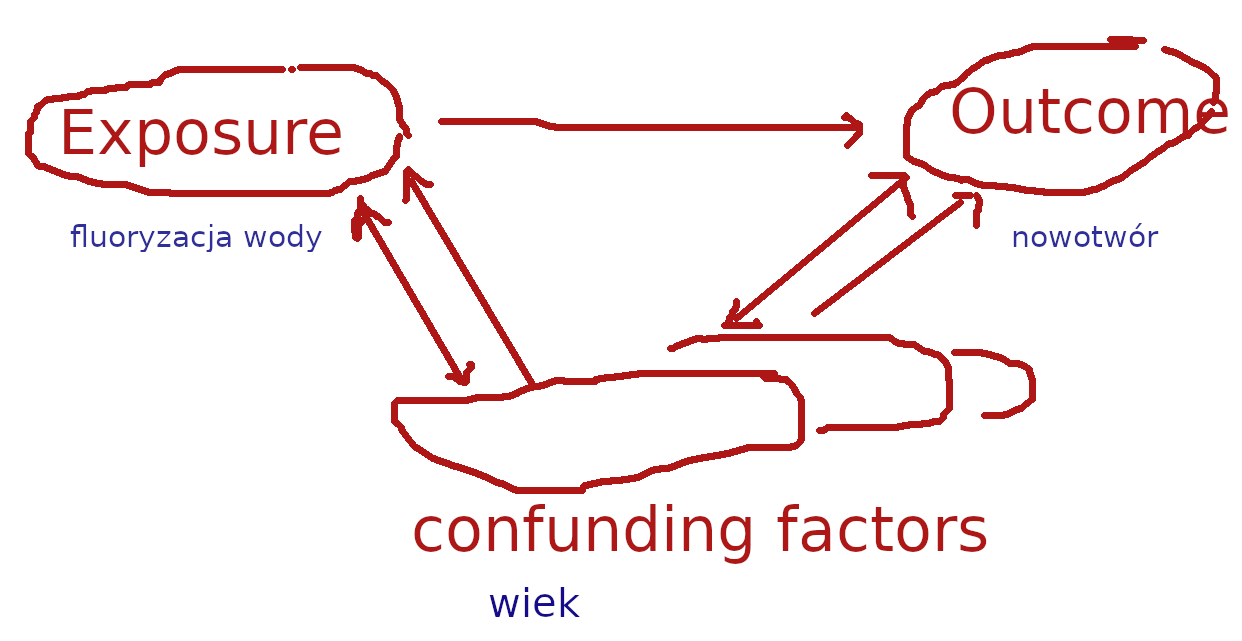
\includegraphics[width=0.99\linewidth]{./Model1_cropped} \caption{Fluoryzacja, wiek a nowotwór}\label{fig:fluor}
\end{figure}

\textbf{Efekt przyczynowy} to \textbf{ilościowe} określenie wpływu
ekspozycji na wynik
poprzez porównanie wielkości wyniku dla różnych wielkości ekspozycji.

Są dwa typy \textbf{efektu przyczynowego}:
indywidualny efekt interwencji (\emph{individual treatment effect}) oraz
średni efekt interwencji (\emph{average treatment effect}).

\textbf{Individual Treatment Effect (ITE)}

Indywidualny efekt interwencji (ITE) określa ilościowo wpływ
interwencji dla konkretnej osoby poprzez porównanie
wyników dla różnych wartości interwencji.

Mogę pić kawę lub nie pić kawy a wynikiem będzie ocena. Oczywiście
nie mogą zrobić tych dwóch rzeczy na raz.

\textbf{Average Treatment Effect (ATE)}

Średni efekt interwencji
określa ilościowo wpływ interwencji dla grupy osób.

W grupie studentów jedni pili kawę inni nie.

Jeżeli grupa (populacja) została uprzednio podzielona (losowo) na
grupę \textbf{eksperymentalną} oraz \textbf{grupę kontrolną}
możemy policzyć ATE oddzielnie dla obu grup.
Wtedy efekt przyczynowy można zdefiniować jako:

ATT - ATC (albo ATT/ATC)

gdzie: ATT oznacza ATE w grupie eksperymentalnej
a ATC oznacza ATE w grupie kontrolnej.

\begin{example}
\textbf{Kawa a ocena (kontynuacja)}

Można przypuszczać, że oprócz kawy na wynik egzaminu ma wpływ np. wrodzone predyspozycje
w dziedzinie intelektualnej oraz czas poświęcony na naukę.
Aby kontrolować ten czynnik można podzielić losowo grupę studentów;
dzięki czemu średnia wielkość predyspozycji oraz czasu w obu grupach będzie podobna.
Następnie zalecamy studentom w \textbf{grupie eksperymentalnej} picie 1l kawy dziennie
a studentom w \textbf{grupie kontrolnej} podajemy 1l brązowej wody o smaku i zapachu kawy :-).
Średnie wyniki w
grupie studentów pijących 1l kawy okazały się wyższe niż w grupie pijącej kolorową wodę.
Czy można powiedzieć że udowodniono
iż picie dużej ilości kawy poprawia wynik egzaminu?
Raczej tak.
\end{example}

\textbf{Badania obserwacyjne} można z kolei podzielić na \textbf{analityczne} i \textbf{opisowe}.

W badaniach \textbf{analitycznych} porównuje się grupę kontrolną z grupą poddaną ekspozycji/leczeniu;
w badaniach przekrojowych nie ma grupy kontrolnej.

Badania analityczne dzielimy dalej na:

\begin{itemize}
\item
  \textbf{kohortowe},
\item
  \textbf{kliniczno-kontrolne},
\item
  \textbf{przekrojowe}.
\end{itemize}

Badanie \textbf{kohortowe} (\emph{cohort study}): wieloletnie badania na dużej grupie jednostek.
Pomiar zaczynamy od ekspozycji kończymy na wyniku/chorobie/zgonie
(takie badanie nazywamy \textbf{prospektywnym}.
Problem: koszty (np. choroby rzadkie wymagają ogromnych kohort).

Badanie \textbf{kliniczno-kontrolne} (\emph{case-control study}): \textbf{retrospektywna} ocena ekspozycji
dla jednostek, u których stwierdzono wynik (chorobę). Grupę kontrolną tworzą \textbf{dopasowane} jednostki
u których wyniku nie stwierdzono (dopasowane w sensie, że są podobne podobne.)
W praktyce badanie kliniczno-kontrolne to badanie chorych, którzy zgłosili się do przychodni;
grupą kontrolną są podobni chorzy (wiek, płeć) z innej przychodni.

Problem1: błąd pamięci (\emph{recall bias}) pacjenci -- zwłaszcza zdrowi -- słabo pamiętają
fakty które miały miejsce lata temu.
Problem2: trudności z \textbf{dopasowaniem} grupy kontrolnej (łatwiej powiedzieć niż zrobić).

Badania \textbf{prospektywne}: od przyczyny do skutku (\emph{cohort}); badanie \textbf{retrospektywne}:
od skutku do przyczyny (\emph{case-control}).

Badanie przekrojowe (\emph{cross-sectional study}): badanie związku między wynikiem a ekspozycją
bez podziału na grupę eksperymentalną i kontrolną.

Problem: nie da się określić związku przyczyna-skutek w taki sposób jaki się stosuje w badaniach analitycznych,
ale można do tego celu zastosować \textbf{model} regresji liniowej.

\begin{example}
\textbf{Palenie a nowotwór}

Badamy grupę pacjentów przychodni onkologicznej. Stwierdzamy że 90\% z nich paliło
papierosy. Czy z tego wynika że palenie powoduje raka? Niekoniecznie. Możemy \textbf{dopasować}
pacjentów o podobnym profilu demograficzno-społecznym z innej przychodni (którzy nie chorują na raka)
i stwierdzić że 20\% z nich paliło.
To już jest konkretny argument -- ale takie badanie nie jest już \textbf{przekrojowe}
tylko \textbf{kliniczno-kontrolne}.
\end{example}

\begin{example}
\textbf{Kawa a ocena (kontynuacja)}

Można oprócz pytania studentów o ilość kawy i wynik pytać ich jeszcze o czas poświęcony
na naukę oraz o średnią ze studiów (wrodzone predyspozycje w dziedzinie intelektualnej).
Za pomocą metody regresji możemy ustalić czy i jak bardzo kawa, czas i predyspozycje
wpływają na ocenę. Teoretycznie zamiast eksperymentu można używać regresji, ale jest to w większości
przypadków trudne -- albo zmienne nie da się zmierzyć (czy średnia ze studiów jest dobrą miarą predyspozycji?)
albo jakąś ważną zmienną pominiemy. Więcej na temat regresji w rozdziale \ref{causality}.
\end{example}

Badanie \textbf{ekologiczne}: badanie (przekrojowe) zależności pomiędzy wielkościami \textbf{zagregowanymi} a \textbf{indywidualnymi}.
Przykładowo wielkości zagregowane, to zależność pomiędzy przeciętną
wielkością dochodu narodowego, a przeciętną oczekiwaną długością życia np. na poziomie kraju.

Problem: błąd ekologizmu (\textbf{ecological fallacy}.) Zależności na poziomie indywidualnym oraz zagregowanym
mogą być różne. Można oczekiwać, że im większy dochód tym osoba dłużej żyje (poziom indywidualny.) Jeżeli
w kraju występują duże różnice w dochodach (na przykład w USA), to przeciętnie dochód jest wysoki, ale jest
dużo osób o niskich dochodach, o ograniczonym dostępie do służby zdrowia, i krótszej oczekiwanej długości życia.
Przeciętna oczekiwana długość życia na poziomie całego kraju jest niższa (bo jest sumą wysokiej
dla bogatych + niskiej dla biednych).
W rezultacie zależność na poziomie zagregowanym może się znacząco różnić
od tej na poziomie indywidualnym.

\hypertarget{przykux142ady-badaux144}{%
\subsection{Przykłady badań}\label{przykux142ady-badaux144}}

Jest ustalony szablon artykułu naukowego, który powinien być podzielony na
następujące części:

\begin{enumerate}
\def\labelenumi{\arabic{enumi}.}
\item
  \textbf{Wprowadzenie}: określenie problemu badawczego, celu badania.
\item
  \textbf{Materiał i metoda}: Opis danych i zastosowanych metod statystycznych.
\item
  \textbf{Wyniki}: Rezultaty analiz.
\item
  \textbf{Dyskusja}: Znaczenie uzyskanych wyników; jeżeli we wstępie postawiono hipotezy
  to tutaj należy przedstawić wyniki ich weryfikacji.
\end{enumerate}

Żeby się zorientować jakie dane (jakie zmienne i jak mierzone) oraz jakie metody statystyczne zostały
wykorzystane w pracy wystarczy zapoznać się z treścią punktu \textbf{materiał i metoda}. W szczególności
powinien tam być określony \textbf{rodzaj badania}: eksperyment, badanie kohortowe, kliniczno-kontrolne,
przekrojowe lub inne.

\begin{example}
\textbf{Czy konsumpcja soli kuchennej szkodzi? (eksperyment)}

Neal B. i inni zastosowali eksperyment kontrolowany do zbadania
wpływu substytucji chlorku sodu chlorkiem potasu na choroby sercowo-naczyniowe
(\emph{Effect of Salt Substitution on Cardioviscular Events and Death,
New England Journal of Medicine},
\url{https://doi.org/10.1056/NEJMoa2105675}). W badaniu
przeprowadzonym w Chinach, uczestniczyli mieszkańcy 600 wsi, podzieleni
losowo na dwie grupy. Uczestnik badania musiał mieć minimum 60 lat oraz
nadciśnienie krwi. W badaniu uczestniczyło prawie 21 tysięcy osób.
Przez pięć lat trwania eksperymentu grupa kontrolna używała soli zawierającej 75\% chlorku potasu oraz 25\%
chlorku sodu; grupa badana zaś używała soli tradycyjnej czyli zawierającej
wyłącznie chlorek sodu. Obserwowano w okresie pięcioletnim w obu grupach
liczbę udarów, incydentów sercowo-naczyniowych oraz zgonów. Wpływ
substytucji oceniono porównując współczynniki ryzyka w obu grupach.
\end{example}

\begin{example}
\textbf{Konflikt praca-dom w zawodzie pielęgniarki (przekrojowe)}

Simon i inni badali konflikt Praca-Dom w zawodzie Pielęgniarki/Pielęgniarza
(Work-Home Conflict in the European Nursing Profession
Michael Simon 1, Angelika Kümmerling, Hans-Martin Hasselhorn; Next-Study Group
Int J Occup Environ Health 2004 Oct-Dec;10(4):384-91. doi: 10.1179/oeh.2004.10.4.384.
\url{https://pubmed.ncbi.nlm.nih.gov/15702752/}).

Konflikt Praca-Dom (WHC) to sytuacja kiedy
nie można zająć się zadaniami lub obowiązkami w jednej dziedzinie ze względu na obowiązki
w drugiej domenie. Teoria zapożyczona z obszaru Nauk o Zarządzaniu zapewne.
Ten konflikt jest mierzony odpowiednią skalą pomiarową składającą się z pięciu pytań.
Czynnikami które WHC mają powodować są: czas pracy,
grafik (w sensie rodzaj etatu/zmianowość),
nacisk-na-nadgodziny (występuje lub nie),
intensywność pracy,
obciążenie emocjonalne oraz jakość zarządzania.
(ostatnie trzy mierzone odpowiednimi skalami pomiarowymi,
czytaj: serią pytań w ankiecie).
Badano 27,603 osoby.
Podstawowym narzędziem badawczym jak się łatwo domyśleć była ankieta,
a przyczyny WHC ustalono za pomocą metody regresji wielorakiej.

Teraz porównajmy koszty badania \#1, w którym jedynie starano się ustalić że sól szkodzi (lub nie)
z badaniem \#2, w którym starano się ustalić przyczyny stanów psychicznych badanych.
\end{example}

\hypertarget{miary-czux119stoux15bci-choruxf3b}{%
\section{Miary częstości chorób}\label{miary-czux119stoux15bci-choruxf3b}}

\textbf{Populacja narażona} (\emph{population at risk}): grupa osób podatnych na zdarzenie (chorobę);
rak szyjki macicy dotyczy kobiet a nie wszystkich.

\textbf{Współczynnik chorobowości} (\emph{prevalence rate}): liczba chorych w określonym czasie (dzień, tydzień, rok) podzielona przez wielkość populacji narażonej.
Ponieważ są to zwykle bardzo małe liczby, mnoży się wynik przez \(10^n\) dla ułatwienia interpretacji.
Czyli jeżeli
chorych w populacji narażonej o wielkości 1mln jest 20 osób, to współczynnik wynosi 20/1mln = 0,000002 co trudno
skomentować po polsku. Jeżeli pomnożymy owe 0,000002 przez 100 tys (\(n=5\)), to współczynnik będzie równy 2,
co interpretujemy jako dwa przypadki na 100 tys.
(albo 0,2 na 10 tys, jeżeli \(n=4\), co już jednak brzmi trochę gorzej).

\textbf{Współczynnik zapadalności} (\emph{incidence rate}): liczba nowych chorych w określonym czasie (dzień, tydzień, rok) podzielona przez wielkość populacji narażonej. Też zwykle pomnożona przez \(10^n\).

\textbf{Współczynnik śmiertelności} (\emph{case fatality rate}): liczba zgonów z powodu X w określonym czasie (dzień, tydzień, rok) podzielona
przez liczbę chorych na X w tym samym czasie. Śmiertelność jest miarą ciężkości choroby X.

\textbf{Współczynnik zgonów} (\emph{death rate}): liczba zgonów w określonym czasie przez średnią
liczbę ludności w tym czasie (pomnożone przez \(10^n\)).

Jeżeli współczynnik zgonów nie uwzględnia wieku, nazywany jest surowym (\emph{crude}); grupy różniące się strukturą wieku
nie powinny być porównywane za pomocą współczynników surowych tylko standaryzowanych (\emph{age-standardized} albo
\emph{age-adjusted}). Przykładowo jeżeli porównamy współczynnik zgonów USA i Nigerii to okaże się że w USA jest wyższy
a to z tego powodu że społeczeństwo amerykańskie jest znacznie starsze (a umierają zwykle ludzie starzy).

\textbf{Współczynnik zgonów} standaryzowany według wieku to ważona średnia współczynników w poszczególnych
grupach wiekowych, gdzie wagami są udziały tychże grup wiekowych w pewnej \textbf{standardowej populacji}.

\hypertarget{oprogramowanie}{%
\section{Oprogramowanie}\label{oprogramowanie}}

Nie da się praktykować statystyki bez korzystania z programów komputerowych
i mamy w tym zakresie trzy możliwości:

\begin{enumerate}
\def\labelenumi{\arabic{enumi}.}
\item
  Arkusz kalkulacyjny. Przydatny na etapie zbierania danych i ich wstępnej
  analizy, później już niekoniecznie. Policzenie niektórych rzeczy jest niemożliwe
  (brak stosownych procedur) lub czasochłonne (w porównaniu do 2--3).
\item
  Oprogramowanie specjalistyczne komercyjne takie jak programy STATA czy SPSS.
  Wady: cena i czas niezbędny na ich poznanie.
\item
  Oprogramowanie specjalistyczne darmowe: Jamovi oraz R.
  Same zalety.
\end{enumerate}

W większości podręczników opisuje się \textbf{procedury}
oraz \textbf{program}, w którym te procedury można zastosować jednocześnie.
My zdecydowaliśmy się oddzielnie przestawić teorię
statystyki (rozdziały \ref{przedmiotbadan}--\ref{surveyexamples})
a oddzielnie opis posługiwania się konkretnym programem (rozdział \ref{intro2jamovi}).

\hypertarget{analiza1z}{%
\chapter{Analiza jednej zmiennej}\label{analiza1z}}

\textbf{Statystyka opisowa} (opis statystyczny) to zbiór metod statystycznych służących do -- surprise, surprise -- opisu
(w sensie przedstawienia sumarycznego) zbioru danych;
w zależności od typu danych (przekrojowe, czasowe, przestrzenne) oraz sposobu pomiaru
(dane nominalne, porządkowe liczbowe) należy używać różnych metod.

W przypadku \textbf{danych przekrojowych} opis statystyczny nazywany jest \textbf{analizą struktury}
i sprowadza się do opisania danych z wykorzystaniem:

\begin{itemize}
\item
  tablic (statystycznych);
\item
  wykresów;
\item
  parametrów (takich jak średnia czy mediana).
\end{itemize}

\textbf{Rozkład zmiennej} (cechy) to przyporządkowanie
wartościom zmiennej odpowiedniej \textbf{liczby wystąpień} w postaci \textbf{liczebności} albo \textbf{częstości}
(popularnych procentów).

\textbf{Analiza struktury} (dla jednej zmiennej) obejmuje:

\begin{itemize}
\item
  \textbf{określenie tendencji centralnej} (\textbf{miary położenia}:
  wartość przeciętna, mediana, dominanta);
\item
  \textbf{zróżnicowanie wartości} (rozproszenie: odchylenie standardowe, rozstęp ćwiartkowy);
\item
  \textbf{asymetrię} (rozłożenie wartości zmiennej wokół średniej).
\end{itemize}

\hypertarget{tablice-statystyczne}{%
\section{Tablice statystyczne}\label{tablice-statystyczne}}

\textbf{Tablica statystyczna} to (w podstawowej formie) dwukolumnowa tabela zawierająca
wartości zmiennej oraz odpowiadające tym wartościom liczebności (i/lub częstości).

\textbf{Tablica dla zmiennej niemierzalnej (nominalnej albo porządkowej)}.

\begin{example}
\textbf{Absolwenci studiów pielęgniarskich w ośmiu największych krajach UE}

Tablica: Absolwenci studiów pielęgniarskich w ośmiu największych
krajach UE w roku 2018

\begin{tabular}{lr}
\toprule
kraj & liczba absolwentów\\
\midrule
Belgium & 7203\\
Germany & 35742\\
Spain & 9936\\
France & 25757\\
Italy & 11207\\
\addlinespace
Netherlands & 9920\\
Poland & 9070\\
Romania & 18664\\
\bottomrule
\end{tabular}

Źródło: Eurostat, tablica Health graduates (HLTH\_RS\_GRD)
\end{example}

W przykładzie \textbf{jednostką statystyczną} jest absolwent studiów pielęgniarskich
w roku 2018,
badaną \textbf{zmienną} zaś \textbf{kraj w którym ukończył studia}.

\textbf{Tablica dla zmiennej mierzalnej liczbowej skokowej}

Przypomnijmy, że zmienna skokowa to taka zmienna, która
może przyjąć skończoną (przeliczalną) liczbę wartości.

Jeżeli tych wartości jest mało, to tablica zawiera wyliczenie
wartości zmiennej i odpowiadających im liczebności. Jeżeli liczba wariantów
zmiennej jest duża, to tablica zawiera klasy wartości (przedziały wartości)
oraz odpowiadające im liczebności.

Liczba przedziałów jest dobierana metodą prób i błędów, tak aby:

\begin{itemize}
\item
  przedziały wartości były jednakowej rozpiętości;
\item
  Na zasadzie wyjątku dopuszcza się aby pierwszy i ostatni przedział
  były \textbf{otwarte}, tj. nie miały dolnej (pierwszy) lub górnej (ostatni) \textbf{granicy};
\item
  nie było przedziałów z zerową liczebnością;
\item
  przedziałów nie było za dużo ani za mało (typowo 5--15);
\item
  większość populacji nie znajdowała się w jednym albo dwóch przedziałach.
\end{itemize}

\begin{example}
\textbf{Gospodarstwa domowe wg liczby osób}

Tablica: Gospodarstwa domowe w mieście Kwidzyn wg liczby osób w roku 2021

\begin{tabular}{lrr}
\toprule
liczba osób & liczba gospodarstw & \%\\
\midrule
1 & 2790 & 21,64972\\
2 & 3420 & 26,53837\\
3 & 2618 & 20,31505\\
4 & 2246 & 17,42842\\
5 i więcej & 1813 & 14,06844\\
\addlinespace
razem & 12887 & 100,00000\\
\bottomrule
\end{tabular}

Źródło: Bank danych lokalnych GUS, podgrupa P4287/Gospodarstwa domowe według liczby osób
\end{example}

W powyższym przykładzie druga kolumna tablicy zawiera liczebności a trzecia częstości (udziały procentowe).
W 1813 gospodarstwach domowych mieszkało 5 i więcej osób co stanowiło 14,1\% wszystkich
gospodarstw domowych w mieście Kwidzyn.

\textbf{Tablica dla zmiennej mierzalnej liczbowej ciągłej}

Przypomnijmy, że zmienna ciągła to taka zmienna, która może przyjąć nieskończoną i nieprzeliczalną
liczbę wartości.

Tablica zawiera klasy (przedziały) wartości
oraz odpowiadające im liczebności.

Liczba przedziałów jest dobierana metodą prób i błędów, tak aby:

\begin{itemize}
\item
  przedziały wartości były jednakowej rozpiętości;
\item
  Na zasadzie wyjątku dopuszcza się aby pierwszy i ostatni przedział
  były \textbf{otwarte}, tj. nie miały dolnej (pierwszy) lub górnej (ostatni) \textbf{granicy};
\item
  nie było przedziałów z zerową liczebnością;
\item
  przedziałów nie było za dużo ani za mało (typowo 8--15);
\item
  większość populacji nie znajdowała się w jednej czy dwóch przedziałach;
\item
  zwykle przyjmuje się za końce przedziałów \textbf{okrągłe liczby}
  bo dziwnie
  by wyglądało gdyby koniec przedziału np. był równy 1,015 zamiast 1,0.
\end{itemize}

\begin{example}
\textbf{Dzietność kobiet na świecie}

Współczynnik dzietności (\emph{fertility ratio} albo FR) -- przeciętna liczba urodzonych dzieci przypadająca
na jedną kobietę w wieku rozrodczym (15--49 lat).
Przyjmuje się, iż FR między 2,10--2,15 zapewnia zastępowalność pokoleń.

Dane dotyczące dzietności dla wszystkich krajów świata pobrano
ze strony \url{https://ourworldindata.org/grapher/fertility-rate-complete-gapminder}).

Zbudujmy tablicę przedstawiającą rozkład współczynników dzietności w roku 2018.
Wszystkich krajów jest \text{201}. Wartość minimalna współczynnika wynosi \text{1,22}, a wartość
maksymalna to \text{7,13}. Decydujemy się na rozpiętość przedziału równą 0,5;
dolny koniec pierwszego przedziału przyjmujemy jako 1,0.

Tablica: Kraje świata według współczynnika dzietności (2018)

\begin{tabular}{lr}
\toprule
Wsp. dzietności & liczba krajów\\
\midrule
(1,1,5] & 24\\
(1,5,2] & 61\\
(2,2,5] & 40\\
(2,5,3] & 17\\
(3,3,5] & 8\\
\addlinespace
(3,5,4] & 15\\
(4,4,5] & 11\\
(4,5,5] & 12\\
(5,5,5] & 6\\
(5,5,6] & 5\\
\addlinespace
(6,6,5] & 1\\
(7,7,5] & 1\\
\bottomrule
\end{tabular}

Źródło: \url{https://ourworldindata.org/grapher/fertility-rate-complete-gapminder}
\end{example}

Zapis \texttt{(1,1.5{]}} oznacza przedział od 1,0 do 1,5 przy czym dolny koniec nie należy
do przedziału a górny 1,5 należy. Który koniec „wchodzi``, a który nie powinien być
jasno oznaczony. Zwykle jest tak jak w przykładzie: górny „wchodzi``, dolny „nie wchodzi``.

Każda tablica statystyczna \textbf{musi} mieć:

\begin{enumerate}
\def\labelenumi{\arabic{enumi}.}
\item
  Część liczbową (kolumny i wiersze);

  \begin{itemize}
  \tightlist
  \item
    żadna rubryka w części liczbowej nie może być pusta (żelazna zasada);
    w szczególności brak danych należy zaznaczyć umownym symbolem.
  \end{itemize}
\item
  Część opisową:

  \begin{itemize}
  \tightlist
  \item
    tytuł tablicy;
  \item
    nazwy (opisy zawartości) wierszy;
  \item
    nazwy (opisy zawartości) kolumn;
  \item
    wskazanie źródła danych;
  \item
    ewentualne uwagi odnoszące się do danych liczb.
  \end{itemize}
\end{enumerate}

Pominięcie czegokolwiek z powyższego jest \textbf{ciężkim błędem}. Jeżeli
nie ma danych (a często -- z różnych powodów -- nie ma, należy to zaznaczyć a nie pozostawiać pustą rubrykę).

\hypertarget{wykresy}{%
\section{Wykresy}\label{wykresy}}

\textbf{Wykresy statystyczne} są graficzną formą prezentacji materiału
statystycznego, są mniej precyzyjne i szczegółowe niż tablice,
natomiast bardziej sugestywne.

Celem jest pokazanie rozkładu wartości zmiennej w populacji: jakie wartości występują
często a jakie rzadko, jak bardzo wartości różnią się między sobą. Jak różnią
się rozkłady dla różnych, ale logicznie powiązanych populacji
(np rozkład czegoś-tam w kraju A i B albo w roku X, Y i Z).

Do powyższego celu celu stosuje się:

\begin{itemize}
\item
  \textbf{wykres słupkowy} (skala nominalna/porządkowa);
\item
  \textbf{wykres kołowy} (skala nominalna/porządkowa);
\item
  \textbf{histogram} (albo wykres słupkowy dla skal nominalnych).
\end{itemize}

Uwaga: \textbf{wykres kołowy} jest
zdecydowanie gorszy od wykresu słupkowego i nie jest zalecany.
\textbf{Każdy} wykres kołowy można wykreślić jako słupkowy i w takiej postaci
będzie on bardziej zrozumiały i łatwiejszy w interpretacji.

Podobnie jak tablice, rysunki powinny być opatrzone tytułem
oraz zawierać źródło wskazujące na pochodzenie danych
(zobacz przedstawione przykłady).

\hypertarget{skala-nominalna-i-porzux105dkowa}{%
\subsection{Skala nominalna i porządkowa}\label{skala-nominalna-i-porzux105dkowa}}

\textbf{Wykres słupkowy (\emph{bar chart})}

Na wykresie słupkowym długość każdego prostokąta (\textbf{słupka}) jest proporcjonalna
do liczebności, którą reprezentuje. Wartości zmiennej (etykiety) są umieszczane pod lub obok słupka.
Słupki można rysować pionowo lub poziomo (jako na powyższym przykładzie). Jeżeli etykiety są długie,
to należy słupki rysować poziomo,
bo wtedy można zmieścić etykiety bez potrzeby ich obracania o 90° czy skracania.

\begin{example}
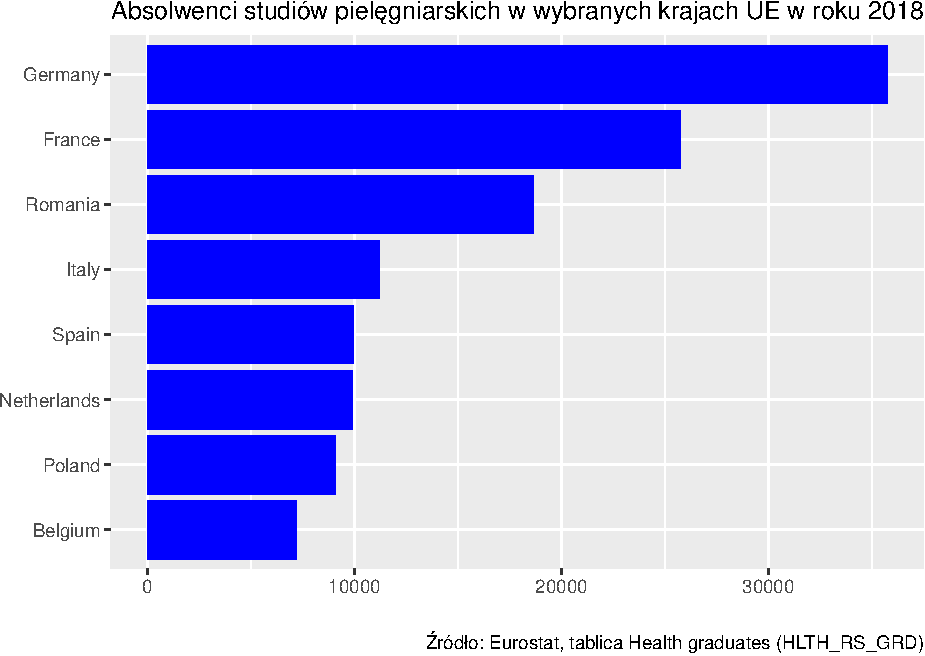
\includegraphics[width=0.85\linewidth]{_main_files/figure-latex/unnamed-chunk-6-1}
\end{example}

\textbf{Wykres kołowy (\emph{pie chart})}

Na wykresie kołowym długość łuku każdego wycinka (a także kąt środkowy oraz pole wycinka)
jest proporcjonalna do liczebności,
którą reprezentuje. Łącznie wszystkie wycinki tworzą pełne koło.

\begin{example}
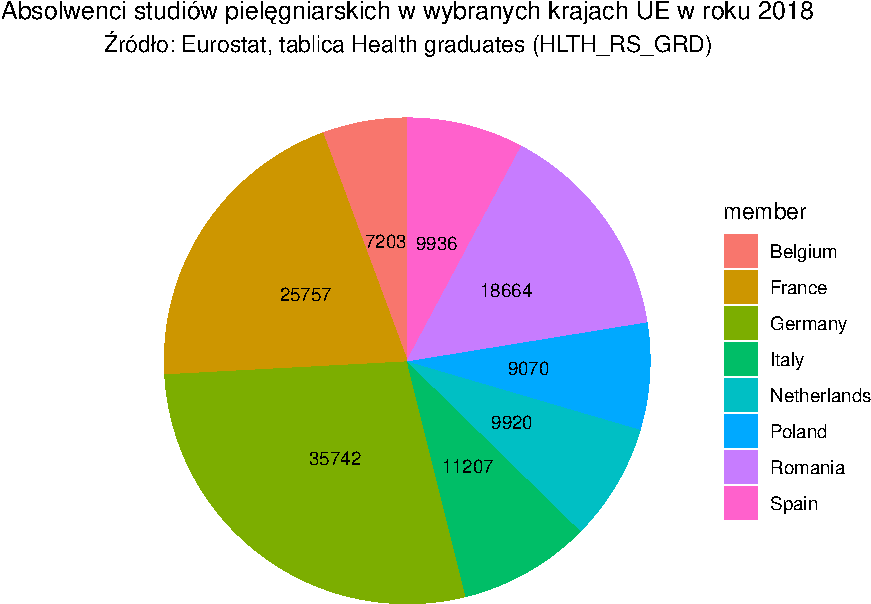
\includegraphics[width=0.85\linewidth]{_main_files/figure-latex/unnamed-chunk-7-1}
\end{example}

Wykres słupkowy i kołowy przedstawiają dokładnie to samo, zatem który wybrać?

Wykres kołowy wygląda zapewne efektowniej (z uwagi na paletę kolorów),
ale jest mniej efektywny. Wymaga dodania legendy, która utrudnia
interpretację treści.
Jeżeli zwiększymy liczbę krajów, to wykres kołowy staje się zupełnie nieczytelny,
bo brakuje rozróżnialnych kolorów, a wycinki koła są zbyt wąskie żeby cokolwiek wyróżniały:

\begin{example}
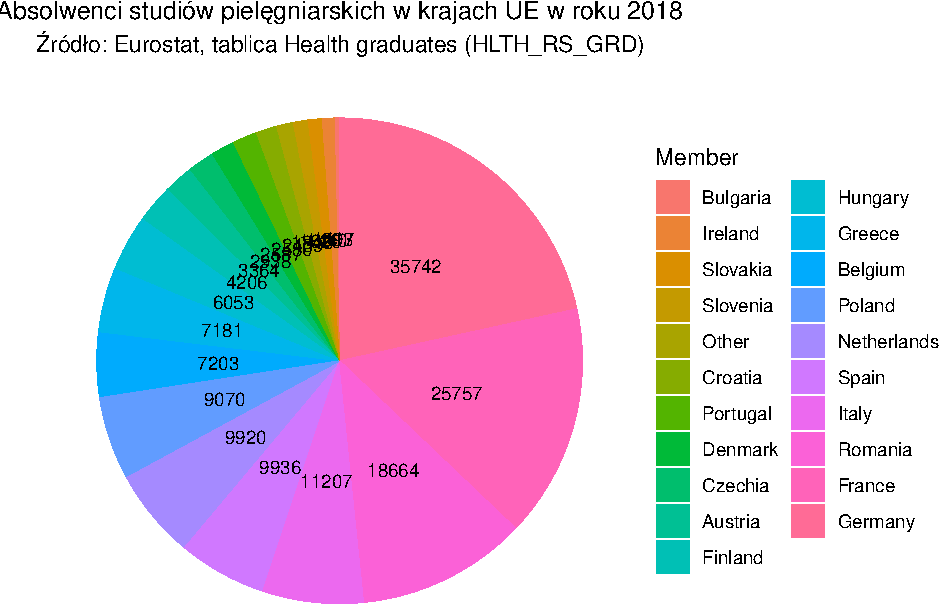
\includegraphics[width=0.85\linewidth]{_main_files/figure-latex/unnamed-chunk-8-1}

Wykres słupkowy dalej jest natomiast OK:

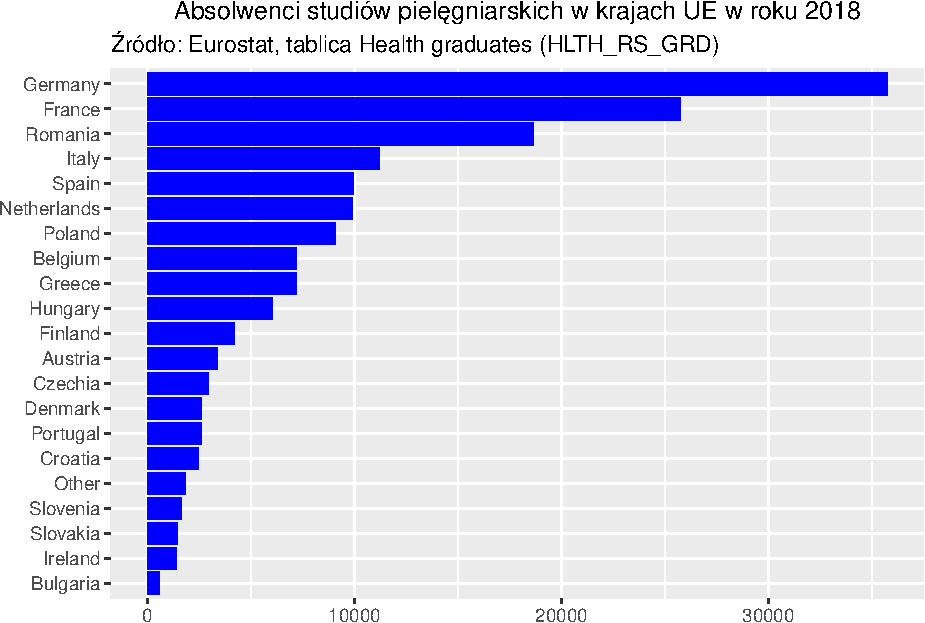
\includegraphics[width=0.85\linewidth]{_main_files/figure-latex/unnamed-chunk-9-1}
\end{example}

\hypertarget{skala-liczbowa}{%
\subsection{Skala liczbowa}\label{skala-liczbowa}}

Histogram to coś w rodzaju wykresu słupkowego tylko na osi OX zamiast
wariantów zmiennej są przedziały wartości.

\begin{example}
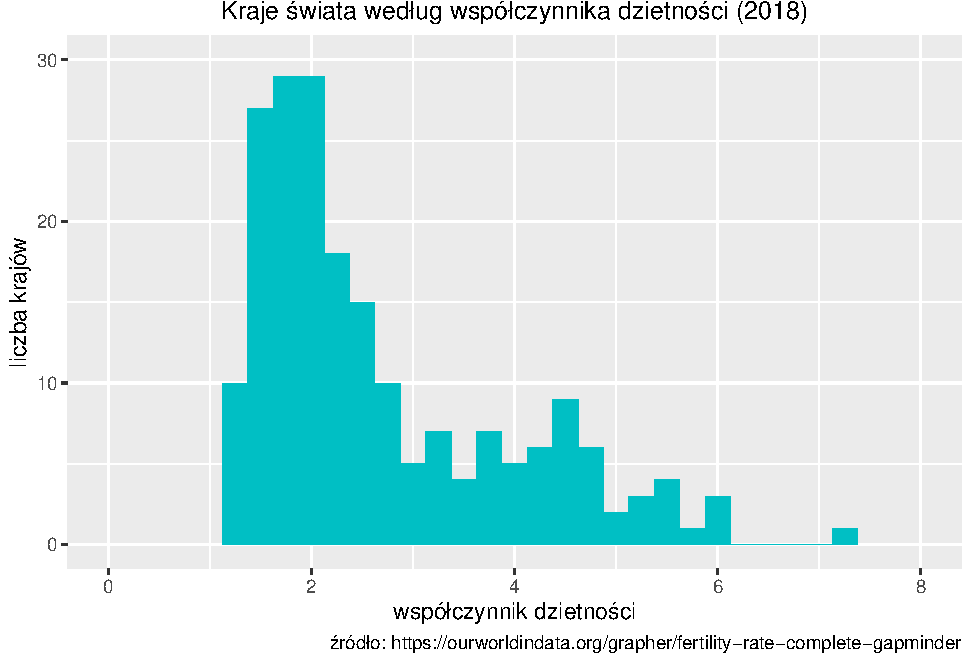
\includegraphics[width=0.85\linewidth]{_main_files/figure-latex/unnamed-chunk-10-1}
\end{example}

Im więcej przedziałów (mniejsza rozpiętość przedziału),
tym histogram jest bardziej szczegółowy
co niekoniecznie
jest pożądane bo zaciemnia ogólny obraz. Nie ma złotych recept na to ile powinno być przedziałów,
a ich liczba determinuje kształt oraz optyczną wielkość histogramu.
Im mniej przedziałów tym histogram będzie optycznie większy.

\hypertarget{fnightingale}{%
\section{Statystyczka Florence Nightingale}\label{fnightingale}}

Nie każdy, kto wie kim była Florence Nightingale, wie że
była ona także statystykiem. W czasie wojny krymskiej nie tylko
zorganizowała opiekę nad rannymi żołnierzami, ale również
-- aby przekonać swoich przełożonych do zwiększenia nakładów na szpitale polowe
-- prowadziła staranną ewidencję szpitalną oraz
zgromadzone dane potrafiła analizować, używając wykresów własnego projektu.

W szczególności słynny jest diagram Nightingale zwane także
różą Nightingale (rys. \ref{fig:nightingale}), które wprawdzie
(podobno) nie okazały się szczególnie użyteczny, no ale nie każdy nowy
pomysł jest od razu genialny:

\begin{figure}
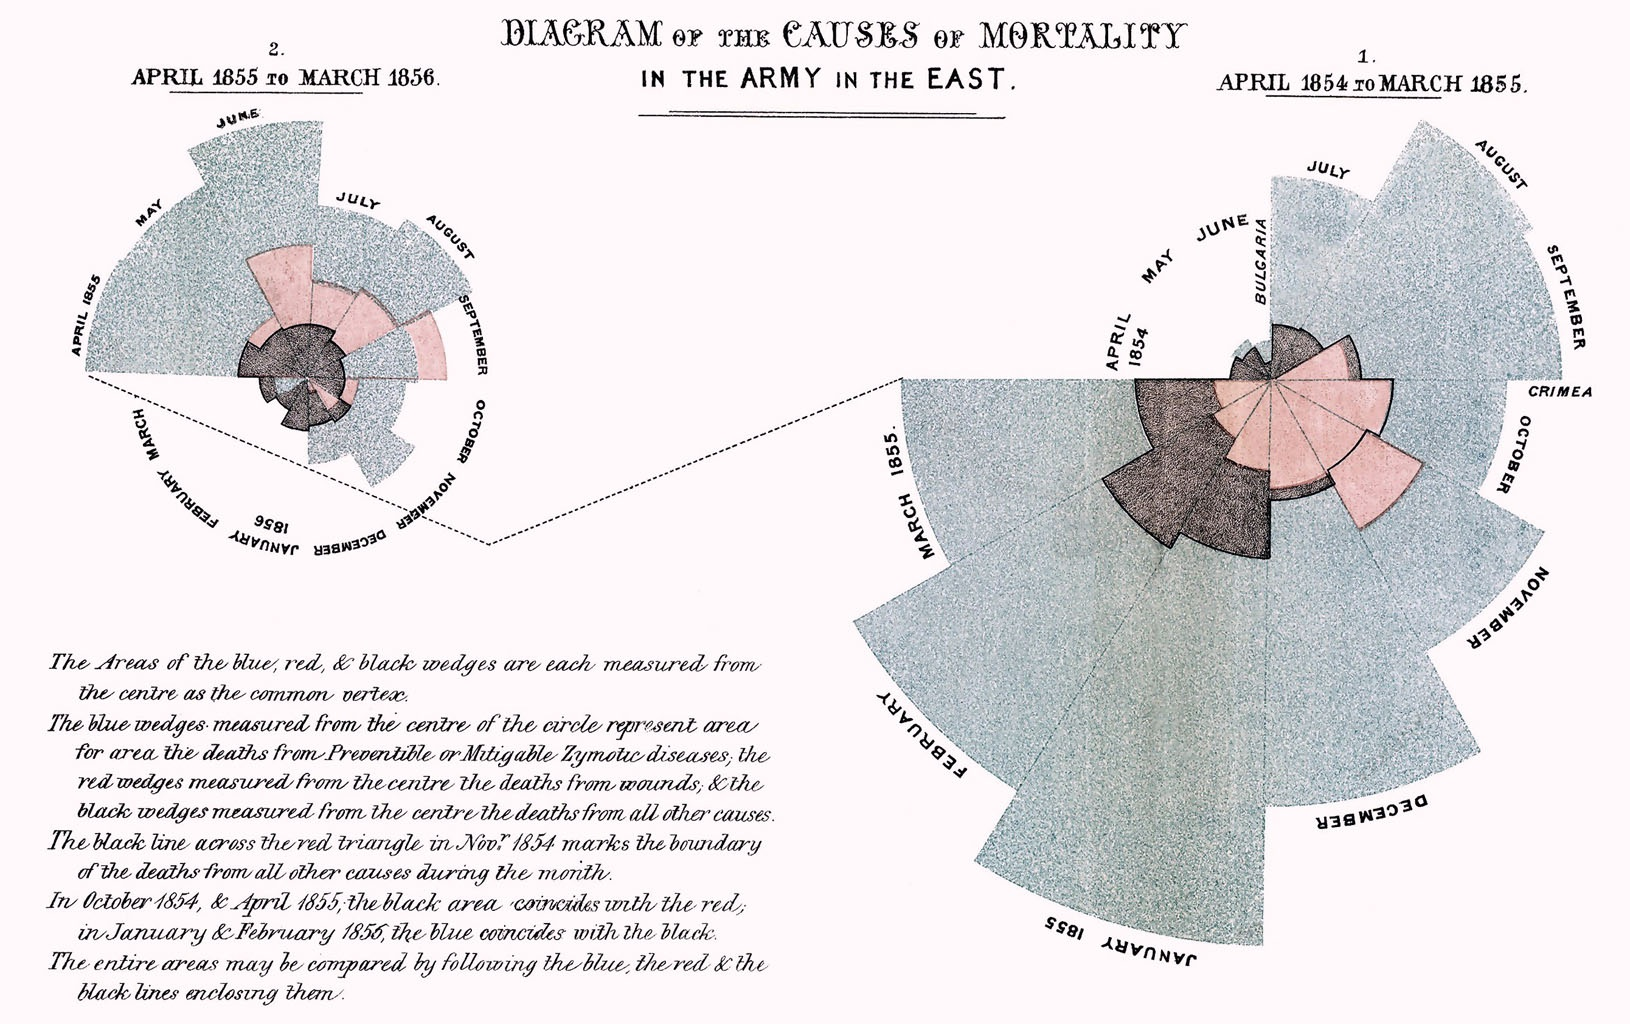
\includegraphics[width=0.9\linewidth]{./FN_diagram} \caption{Róża Nightingale}\label{fig:nightingale}
\end{figure}

Jest to coś w rodzaju wykresu słupkowego tyle że zamiast słupków są wycinki koła. Wycinków jest dwanaście tyle ile miesięcy.
Długość promienia a co za tym idzie wielkość pola wycinka zależy od wielkości zjawiska,
który reprezentuje (przyczyna śmierci: rany/choroby/inne).

Wpisując Florence+Nightingale można znaleźć dużo informacji
na temat, w tym: \url{http://www.matematyka.wroc.pl/ciekawieomatematyce/pielegniarka-statystyczna}.

W 1859 roku Nightingale została wybrana jako pierwsza kobieta na członka Royal Statistical Society (Królewskie Stowarzyszenie Statystyczne) oraz została honorowym członkiem American Statistical Association (Amerykańskiego Stowarzyszenia Statystycznego).

Więc szanowi czytelnicy wnioski są oczywiste.

\hypertarget{analiza-parametryczna}{%
\section{Analiza parametryczna}\label{analiza-parametryczna}}

Analiza parametryczna z oczywistych względów dotyczy tylko zmiennych
mierzonych na skali liczbowej.

\hypertarget{miary-poux142oux17cenia}{%
\subsection{Miary położenia}\label{miary-poux142oux17cenia}}

Miary przeciętne (\textbf{położenia}) charakteryzują średni lub
typowy poziom wartości zmiennej. Są to więc takie wartości, wokół których
skupiają się wszystkie pozostałe wartości analizowanej zmiennej.

\begin{figure}
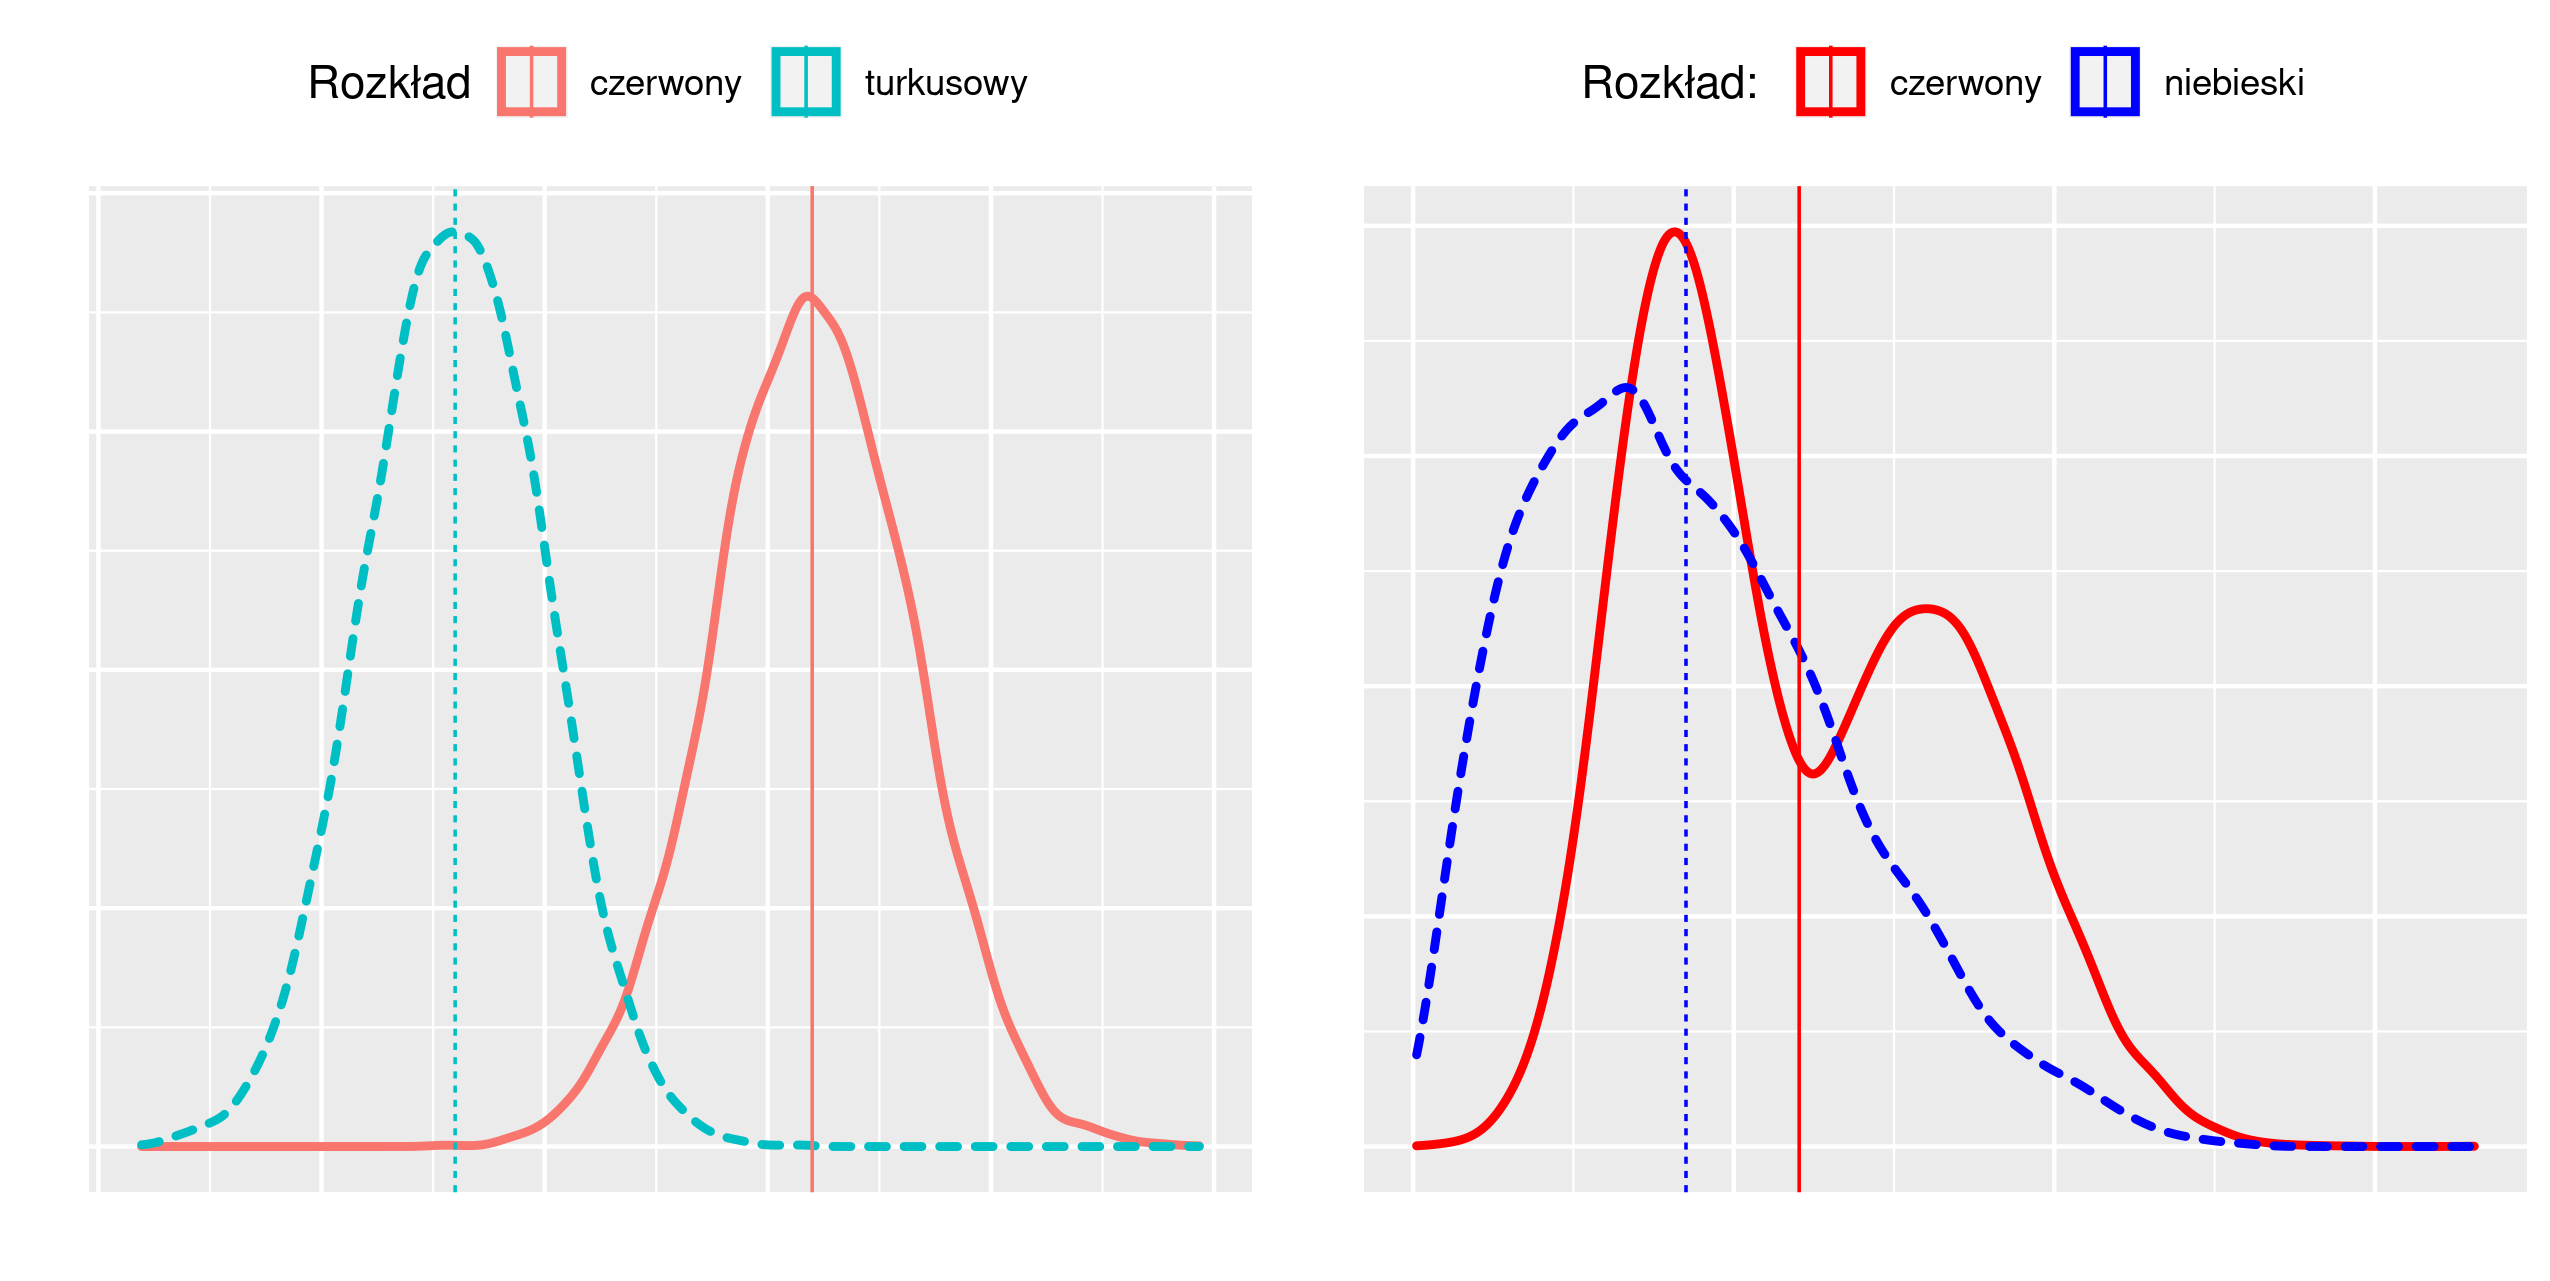
\includegraphics[width=0.99\linewidth]{./distributions} \caption{Rozkłady zmiennej a miary średnie}\label{fig:distributions5}
\end{figure}

Na rysunku \ref{fig:distributions5} po lewej mamy dwa rozkłady różniące się poziomem przeciętnym. Rozkład
czerwony ma przeciętnie większe wartości
niż turkusowy. Są to rozkłady \textbf{jednomodalne},
czyli takie, w których rozkład zmiennej skupia się
wokół jednej wartości.
Dla takich rozkładów ma sens obliczanie średniej arytmetycznej. Te średnie wartości
są zaznaczone na rysunku linią pionową.

Na rysunku po prawej mamy rozkłady \textbf{nietypowe}: \textbf{wielomodalne} (czerwony)
lub \textbf{niesymetryczne} (niebieski). W rozkładzie niesymetrycznym wartości skupiają się nie centralnie,
ale po prawej/lewej od środka przedziału zmienności/wartości średniej).

W świecie rzeczywistym zdecydowana większość rozkładów jest jednomodalna.
Rzadkie przypadki rozkładów wielomodalnych zwykle wynikają z łącznego analizowania
dwóch różniących się wartością średnią zbiorów danych.
Oczywistym zaleceniem w takiej sytuacji jest analiza każdego zbioru oddzielnie.

Rodzaje miar położenia:

\begin{itemize}
\tightlist
\item
  klasyczne:

  \begin{itemize}
  \tightlist
  \item
    \textbf{średnia arytmetyczna},
  \end{itemize}
\item
  pozycyjne:

  \begin{itemize}
  \tightlist
  \item
    \textbf{mediana},
  \item
    \textbf{dominanta},
  \item
    \textbf{kwartyle},
  \item
    ewentualnie kwantyle, decyle, centyle (rzadziej używane).
  \end{itemize}
\end{itemize}

\textbf{Średnia arytmetyczna} (\emph{mean}, \emph{arithmetic mean}), to łączna suma
wartości podzielona przez liczbę sumowanych jednostek. Jeżeli
wartość \(i\)-tej jednostki w zbiorowości o liczebności \(N\) oznaczymy
jako \(x_i\) (gdzie: \(i=1,\ldots, N\)), to średnią można zapisać jako:

\[\bar x = (x_1 + x_2 + \cdots + x_N)/N\]

Uwaga: we wzorach statystycznych zmienne zwykle oznacza się małymi literami
a średnią dla zmiennej przez umieszczenie nad nią kreski poziomej czyli
\(\bar x\) to średnia wartość zmiennej \(x\).

\textbf{Mediana} (\emph{median}, kwartyl drugi) dzieli \textbf{uporządkowaną} zbiorowość na dwie równe części;
połowa jednostek ma wartości zmiennej mniejsze lub równe medianie, a połowa
wartości zmiennej równe lub większe od mediany.
Stąd też mediana bywa nazywana wartością środkową.
Mediana jest oznaczana symbolem Me.

Własności mediany: odporna na wartości nietypowe (w przeciwieństwie do średniej).

\textbf{Dominanta} (\emph{mode}), wartość najczęściej występująca. Jeżeli rozkład jest
wielomodalny to dominanta jest nieokreślona. W szczególności w zbiorowościach
o małej liczebności mogą być problemy z ustaleniem dominanty. Dominanta jest oznaczana
symbolem D lub Mo.

\textbf{Kwartyle} (\emph{quartile}): coś jak mediana tylko bardziej szczegółowo. Kwartyli jest trzy i dzielą
one zbiorowość na 4 równe części, każda zawierająca 25\% całości. Kwartyle oznaczne
są symbolami \(Q_1\), \(Q_2\), \(Q_3\), \(Q_4\).

Pierwszy kwartyl dzieli \textbf{uporządkowaną} zbiorowość w proporcji 25\%--75\%.
Trzeci dzieli \textbf{uporządkowaną} zbiorowość w proporcji 75\%--25\%.
Drugi kwartyl to mediana.

\textbf{Kwantyle} (D, wartości dziesiętne), podobnie jak kwartyle, tyle że dzielą na 10 części.

\textbf{Centyle} (P, wartości setne), podobnie jak kwantyle tyle że dzielą na 100 części.
Przykładowo wartość 99 centyla i mniejszą ma 99\% jednostek w populacji.

\begin{example}
\textbf{Współczynnik dzietności na świecie w roku 2018}

Średnia: \text{2,68}.
Interpretacja: średnia wartość współczynnika dzietności wyniosła
\text{2,68} dziecka.
Mediana: \text{2,2}. Interpretacja mediany: współczynnik dzietności
w połowie krajów na świecie
wynosiła \text{2,2} dziecka i mniej.
Dominanta: \text{1,98}. Interpretacja dominanty: najwięcej krajów wykazuje współczynnik dzietności
równy \text{1,98}. Wartość cokolwiek przypadkowa, bowiem krajów wykazujących
współczynnik równy \text{1,98}, jest raptem \text{4}.

Uwaga: średnia dzietność na świecie \textbf{nie wynosi} \text{2,68} dziecka
(bo po pierwsze uśredniamy kraje a nie kobiety a po drugie kraje różnią się liczbą ludności).
Podobnie dzietność połowy kobiet na świecie wyniosła
\text{2,2} dziecka i mniej jest niepoprawną interpretacją mediany (z tych samych
względów jak w przypadku średniej).
\end{example}

\textbf{Generalna uwaga}: interpretacja średniej-średnich często jest nieoczywista i należy uważać.
(a współczynnik dzietności jest średnią: średnia liczba dzieci urodzonych przez kobietę
w wieku rozrodczym. Jeżeli liczymy średnią dla 202 krajów, to mamy \emph{średnią-średnich}).
Inny przykład: odsetek ludności w wieku poprodukcyjnym wg powiatów (średnia z czegoś takiego
nie da nam odsetka ludności w wieku poprodukcyjnym w Polsce,
bo powiaty różnią się liczbą ludności).

\begin{example}
\textbf{Współczynnik dzietności (kontynuacja)}:

Pierwszy kwartyl: \text{1,75}; trzeci kwartyl \text{3,56} co oznacza że
25\% krajów miało wartość współczynnika dzietności nie większą niż \text{1,75} dziecka
a 75\% krajów miało wartość współczynnika dzietności
nie większą niż \text{3,56} dziecka.
\end{example}

\hypertarget{miary-zmiennoux15bci}{%
\subsection{Miary zmienności}\label{miary-zmiennoux15bci}}

Miary zmienności określają zmienność (dyspersję albo rozproszenie) w zbiorowości.

Rodzaje miar zmienności:

\begin{itemize}
\tightlist
\item
  Klasyczne:

  \begin{itemize}
  \tightlist
  \item
    wariancja i odchylenie standardowe,
  \end{itemize}
\item
  Pozycyjne:

  \begin{itemize}
  \tightlist
  \item
    rozstęp,
  \item
    rozstęp ćwiartkowy.
  \end{itemize}
\end{itemize}

\textbf{Wariancja} (\emph{variance}) jest to średnia arytmetyczna kwadratów
odchyleń poszczególnych wartości zmiennej od średniej arytmetycznej
zbiorowości. Co można zapisać jako (\(\bar x\) oznacza średnią, \(N\) liczebność zbiorowości,
a \(x_i\) wartość \(i\)-tej jednostki):

\[s^2 = \frac{1}{N} \left( (x_1 - \bar x)^2 + (x_2 - \bar x)^2 + 
\cdots +  (x_N - \bar x)^2 \right)\]

Przy czym często zamiast dzielenia przez \(N\) dzielimy przez \(N-1\).

\textbf{Odchylenie standardowe} (\emph{standard deviation}) jest
pierwiastkiem kwadratowym z wariancji. Parametr ten określa
przeciętną różnicę wartości zmiennej od średniej arytmetycznej.
Odchylenie standardowe jest oznaczane symbolem \(s\).

\textbf{Rozstęp ćwiartkowy} (\emph{interquartile range}, IQR) ma banalnie prostą definicję:

\[
R_Q = Q_3 - Q_1
\]
gdzie: \(Q_1\), \(Q_3\) oznaczają odpowiednio pierwszy oraz trzeci kwartyl.

\begin{example}
\textbf{Współczynnik dzietności (kontynuacja)}

Średnie odchylenie od średniej wartości współczynnika
wynosi \text{1,26} dziecka.
Wartość rozstępu ćwiartkowego wynosi \text{1,81} dziecka.
\end{example}

\textbf{Uwaga}: odchylenie standardowe/ćwiartkowe są miarami mianowanymi. Zawsze należy
podać jednostkę miary.

\hypertarget{miary-asymetrii}{%
\subsection{Miary asymetrii}\label{miary-asymetrii}}

Asymetria albo skośność (\emph{skewness}), to odwrotność symetrii. Szereg jest symetryczny
jeżeli jednostki są rozłożone „równomiernie'' wokół wartości średniej.
W szeregu symetrycznym wartości średniej i mediany są sobie równe.
Skośność może być dodatnia (\emph{positive skew}) lub ujemna (\emph{negative skew}).
W przypadku asymetrii prawostronnej większa część zbiorowości przyjmuje wartości
poniżej średniej. W przypadku asymetrii lewostronnej jest odwrotnie.
Rysunek \ref{fig:skeweness} przedstawia rozkład symetryczny oraz rozkłady skośne.

\begin{figure}
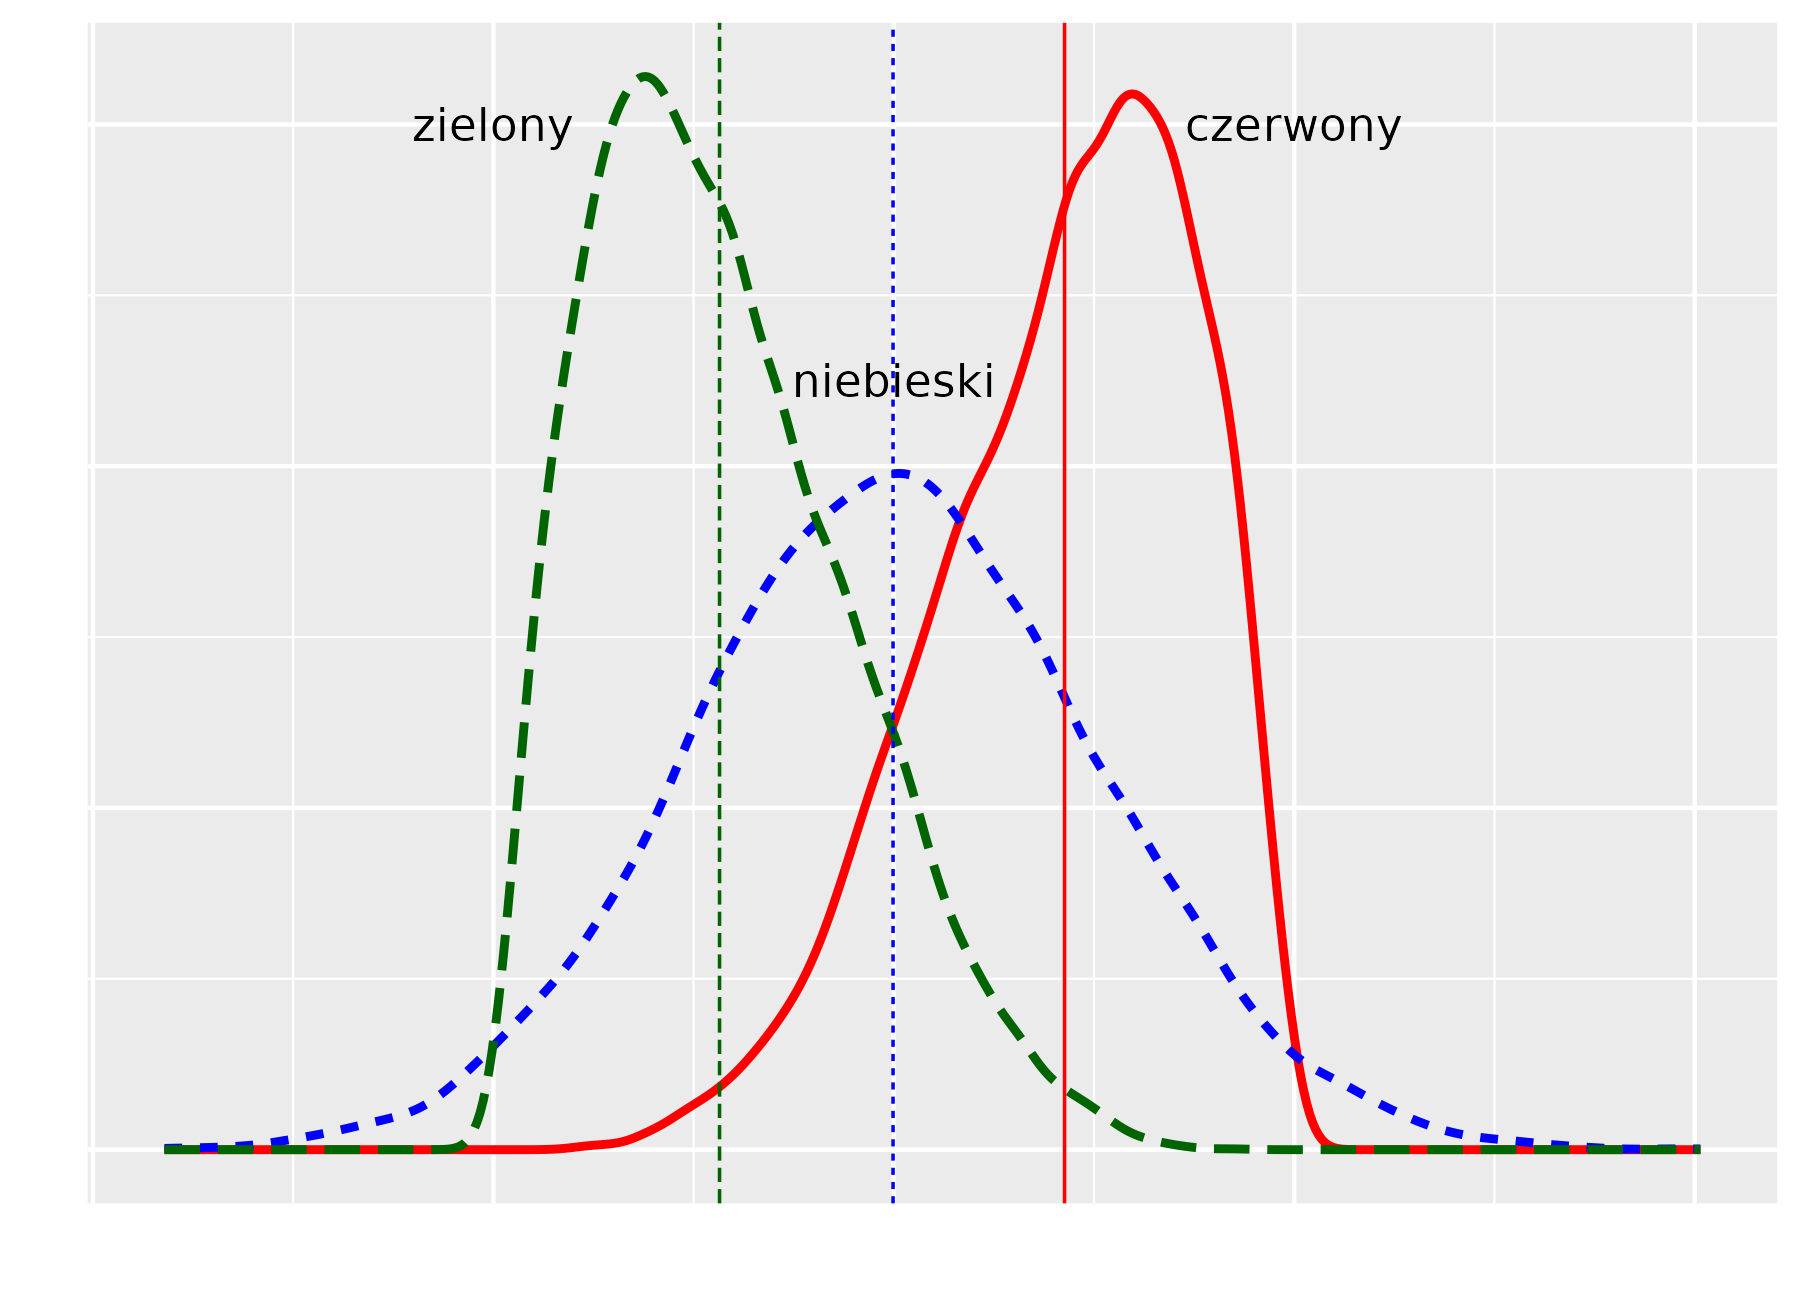
\includegraphics[width=0.99\linewidth]{./neg_posit_screw} \caption{Rozkłady symetryczne i asymetryczne}\label{fig:skeweness}
\end{figure}

Miary asymetrii:

\begin{itemize}
\item
  klasyczny współczynnik asymetrii (\(g\)):

  \begin{itemize}
  \item
    Przyjmuje wartości ujemne dla asymetrii lewostronnej; a dodatnie
    dla prawostronnej. Teoretycznie może przyjąć dowolnie dużą wartość,
    ale w praktyce rzadko przekracza 3 co do wartości bezwzględnej.
  \item
    Wartości większe od 2 świadczą o dużej, a większe od 3 o bardzo dużej
    asymetrii.
  \end{itemize}
\item
  współczynniki asymetrii Pearsona (\(W_s\)):

  \begin{itemize}
  \item
    Wykorzystuje różnice między średnią a dominantą: \(W_s = (\bar x - D)/s\).
  \item
    Wykorzystuje różnice między średnią a medianą: \(W_s = 3(\bar x - Me)/s\).
  \end{itemize}
\item
  Współczynnik asymetrii oparty na odległościach między kwartylami:

  \begin{itemize}
  \tightlist
  \item
    Obliczany jest według następującej
    formuły: \(W_{sq} = ((Q_3 - Q_2) - (Q_2 - Q_1))/ (Q_3 - Q_1)\).
  \end{itemize}
\end{itemize}

\begin{example}
\textbf{Współczynnik dzietności (kontynuacja)}

Współczynnik asymetrii \(g\) wynosi \text{1,1}; Współczynnik
Pearsona wykorzystujący dominantę wynosi \text{0,55}
a wykorzystujący medianę \text{1,14}.
Wreszcie wartość współczynnika opartego o kwartle
wynosi \text{0,5}. Wszystkie współczynniki wskazują
prawostronną (dodatnią) asymetrię. Współczynniki oparte
o dominantę i kwartle wskazują słabą asymetrię, a oparte o medianę
oraz klasyczny umiarkowaną. Jest całkowicie normalne, że różne miary
wykazują różne wartości asymetrii.
\end{example}

\hypertarget{poruxf3wnanie-wielu-rozkux142aduxf3w}{%
\section{Porównanie wielu rozkładów}\label{poruxf3wnanie-wielu-rozkux142aduxf3w}}

Często strukturę jednego rozkładu należy porównać z innym. Albo trzeba porównać
strukturę wielu rozkładów. Pokażemy jak to zrobić na przykładzie.

\begin{example}
\textbf{Masa ciała uczestników Pucharu Świata w Rugby}

W grze w rugby drużyna jest podzielona na dwie \textbf{formacje}: ataku i młyna. Należy porównać
rozkład masy ciała zawodników obu formacji uczestniczących w turniejach o puchar świata w Rugby
w latach 2015, 2019 i 2023.

\textbf{Zawodnicy ataku}

Histogram przy przyjęciu długości przedziału równej \text{4}kg
(pionowa linia zielona oznacza poziom średniej):

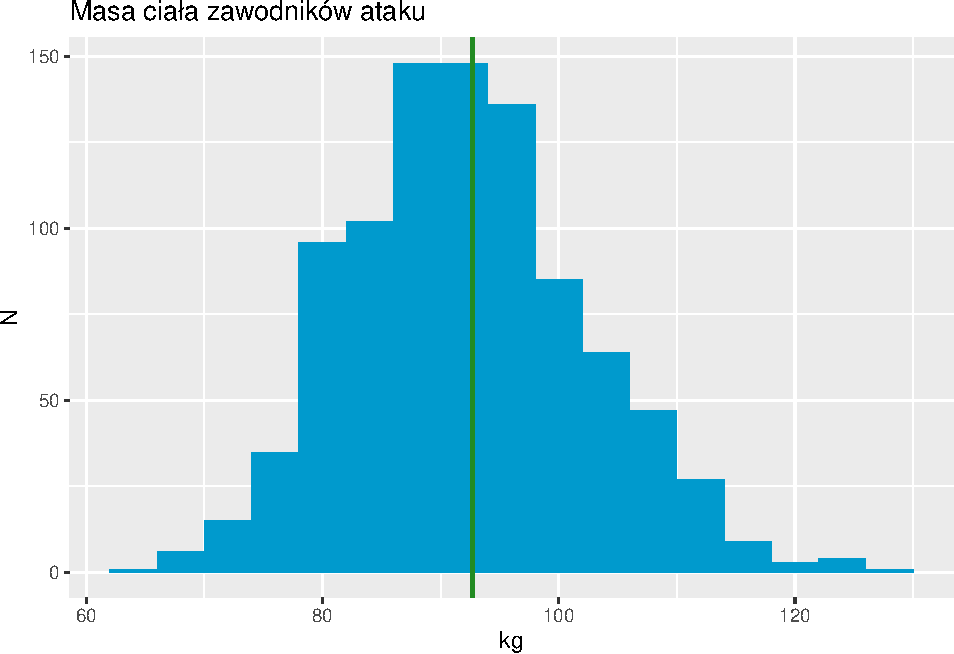
\includegraphics[width=0.85\linewidth]{_main_files/figure-latex/unnamed-chunk-15-1}

Liczba zawodników ataku wyniosła \text{936}.
Przeciętnie zawodnik ataku ważył \text{92,7} kg.
Wartość mediany wyniosła \text{92} kg (połowa
zawodników ataku ważyła \text{92} kg i mniej).
Wartości pierwszego i trzeciego kwartyla wyniosły odpowiednio \text{85,5} oraz \text{99} kg (1/4 zawodników
ataku ważyła \text{85,5} kg i mniej;
1/4 zawodników ataku ważyła \text{99} kg i więcej).

Odchylenie standardowe jest równe \text{10,1} kg (przeciętnie
odchylenie od średniej arytmetycznej wynosi \text{10,1} kg).
Rozstęp ćwiartkowy wynosi \text{13,5} kg (rozstęp 50\% środkowych wartości
wynosi \text{13,5} kg).

Wartość klasycznego współczynnika skośności jest równa \text{0,34}.
Wartość współczynnika skośności opartego o kwartle wynosi \text{0,04},
a współczynnika skośności Pearsona wykorzystującego medianę wynosi \text{0,21}.

\textbf{Zawodnicy młyna}

Histogram przy przyjęciu długości przedziału równej \text{4}kg
(pionowa linia zielona oznacza poziom średniej):

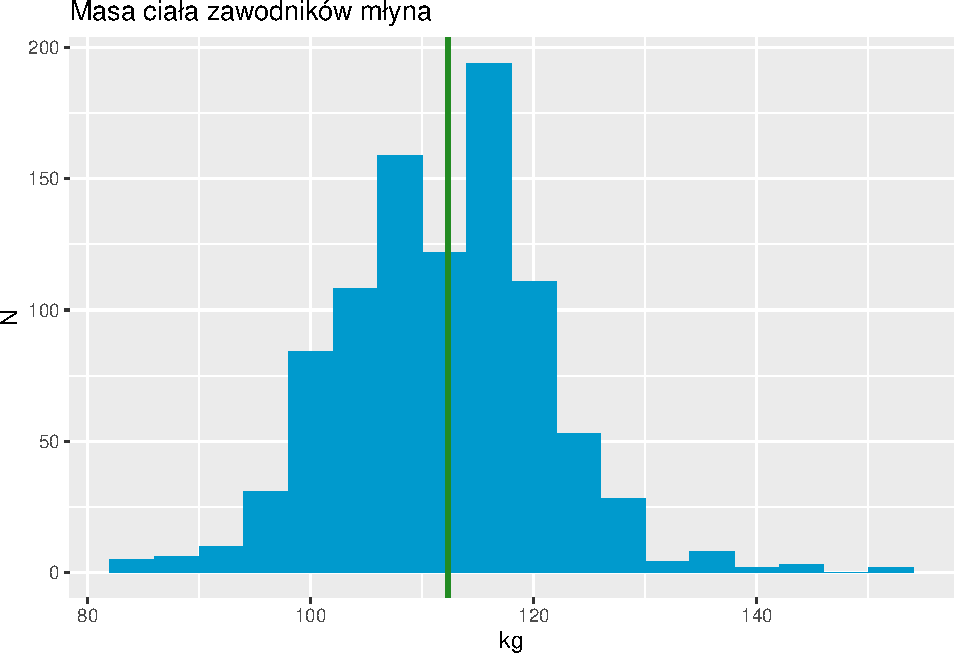
\includegraphics[width=0.85\linewidth]{_main_files/figure-latex/unnamed-chunk-17-1}

Liczba zawodników młyna wyniosła \text{943}.
Średnio zawodnik młyna ważył \text{112,3} kg.
Wartość mediany wyniosła \text{112} kg (połowa zawodników
młyna ważyło \text{112} kg i mniej). Wartości
pierwszego i trzeciego kwartyla wyniosły odpowiednio \text{106} oraz \text{118} kg (1/4 zawodników
młyna ważyło \text{106} kg i mniej;
1/4 zawodników młyna ważyło \text{118} kg i więcej).

Odchylenie standardowe jest równe \text{9,2} kg (przeciętnie
odchylenie od średniej arytmetycznej wynosi \text{9,2} kg).
Rozstęp ćwiartkowy wynosi \text{12} kg (rozstęp 50\% środkowych wartości
wynosi \text{12} kg).

Wartość klasycznego współczynnika skośności jest równa \text{0,17}.
Wartość współczynnika skośności opartego o kwartle wynosi \text{0},
a współczynnika skośności Pearsona wykorzystującego medianę wynosi \text{0,11}.

\textbf{Porównanie atak vs młyn}

\begin{tabular}{lrr}
\toprule
miara & atak & młyn\\
\midrule
średnia & 92,71 & 112,33\\
mediana & 92,00 & 112,00\\
odchyl.st & 10,07 & 9,24\\
iqr & 13,50 & 12,00\\
skośność & 0,34 & 0,17\\
\bottomrule
\end{tabular}

Średnio zawodnik młyna ważył prawie 20 kg więcej od zawodnika ataku (w przypadku mediany
jest to dokładnie 20 kg więcej).
Zmienność mierzona wielkością odchylenia standardowego oraz IQR jest w obu grupach podobna.
Oba rozkłady są zbliżone do rozkładu symetrycznego.

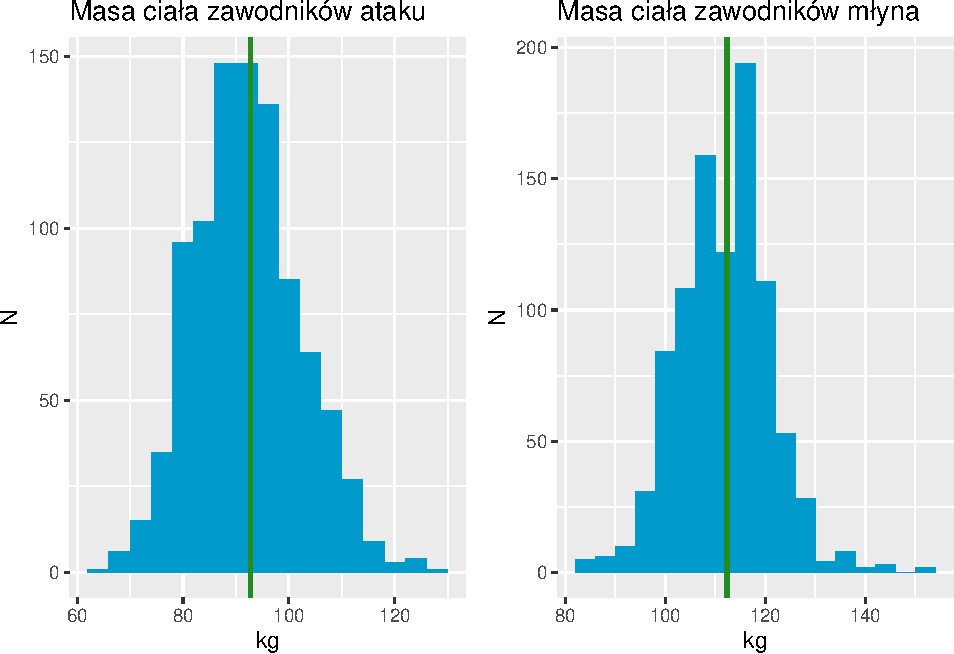
\includegraphics{_main_files/figure-latex/unnamed-chunk-19-1.pdf}
\end{example}

\hypertarget{wykres-pudeux142kowy}{%
\subsection{Wykres pudełkowy}\label{wykres-pudeux142kowy}}

Do porównania wielu rozkładów szczególnie użyteczny jest wykres zwany pudełkowym (\emph{box-plot}).

Pudełka na wykresie pudełkowym są rysowane według następujących zasad
(por rysunek \ref{fig:boxplot}):

\begin{itemize}
\tightlist
\item
  lewy i prawy bok pudełka jest równy kwartylom;
\item
  linia pionowa w środku pudełka jest równa medianie;
\item
  linie poziome (zwane wąsami) mają długość równą \(Q_1 - 1,5 \textrm{IQR}\)
  oraz \(Q_3 + 1,5 \textrm{IQR}\)
  (dla przypomnienia: \(Q_1\), \(Q_3\) to kwartyle, zaś \(\textrm{IQR}\) to rozstęp ćwiartkowy);
\item
  kropki przed oraz za wąsami to wartości zmiennej większe od
  \(Q_3 + 1,5 \textrm{IQR}\) lub mniejsze od \(Q_1 - 1,5 \textrm{IQR}\).
\end{itemize}

\begin{figure}
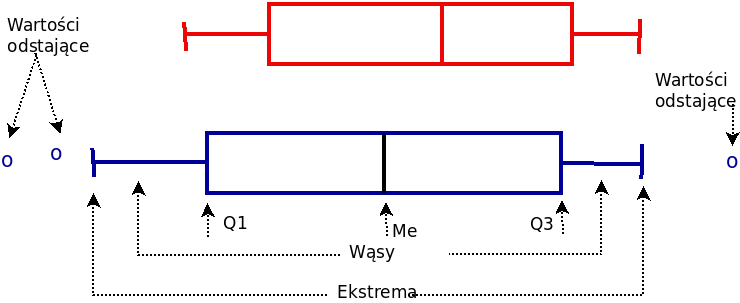
\includegraphics[width=0.99\linewidth]{./boxPlotExample} \caption{Wykres pudełkowy}\label{fig:boxplot}
\end{figure}

Interpretacja pudełek:

\begin{itemize}
\tightlist
\item
  linia pozioma w środku pudełka określa przeciętny poziom zjawiska;
\item
  długość pudełka oraz wąsów określa zmienność (im większe wąsy/długość pudełka
  tym większa zmienność);
\item
  kropki przed oraz za wąsami
  to \textbf{obserwacje nietypowe} (albo \textbf{wartości odstające}).
\end{itemize}

Zatem dolny rozkład z rysunku \ref{fig:boxplot} ma mniejszą wartość
średnią oraz większą zmienność od rozkładu górnego. Dolny
rozkład posiada też wartości odstające, a górny nie.

Zwróć uwagę na następującą sztuczkę. Wartości nietypowe nie są definiowane jako na przykład górne/dolne
1\% wszystkich wartości, bo wtedy \textbf{każdy rozkład} miałby wartości nietypowe,
ale jako wartości mniejsze lub większe od \(Q_{1,3} \pm 1,5 \cdot \mathrm{IQR}\).
Wszystkie wartości rozkładów o umiarkowanej zmienności mieszczą się wewnątrz tak zdefiniowanego przedziału.

Typowo wykres zawiera wiele pudełek, a każde pudełko wizualizuje jeden rozkład. Pudełka
mogą być umieszczone jedno pod drugim, tak jak na rysunku \ref{fig:boxplot} lub
jedno obok drugiego jak na przykładach poniżej.

\begin{example}
\textbf{Masa ciała rugbystów}

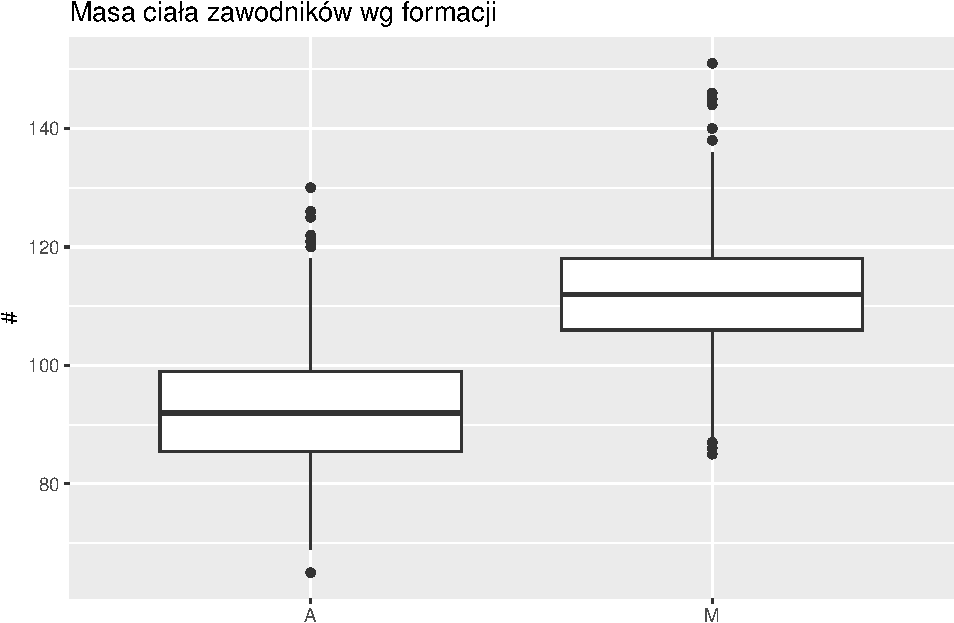
\includegraphics[width=0.95\linewidth]{_main_files/figure-latex/unnamed-chunk-20-1}
\end{example}

Z wykresu od razu widać, który rozkład ma wyższą średnią (M), który większe
rozproszenie (A), oraz w którym występują wartości nietypowe.

Pudełek może być więcej niż dwa oczywiście. Następny przykład
pokazuje
porównanie rozkładów masy ciała zawodników rugby na poszczególnych turniejach.

\begin{example}
\textbf{Masa ciała rugbystów}

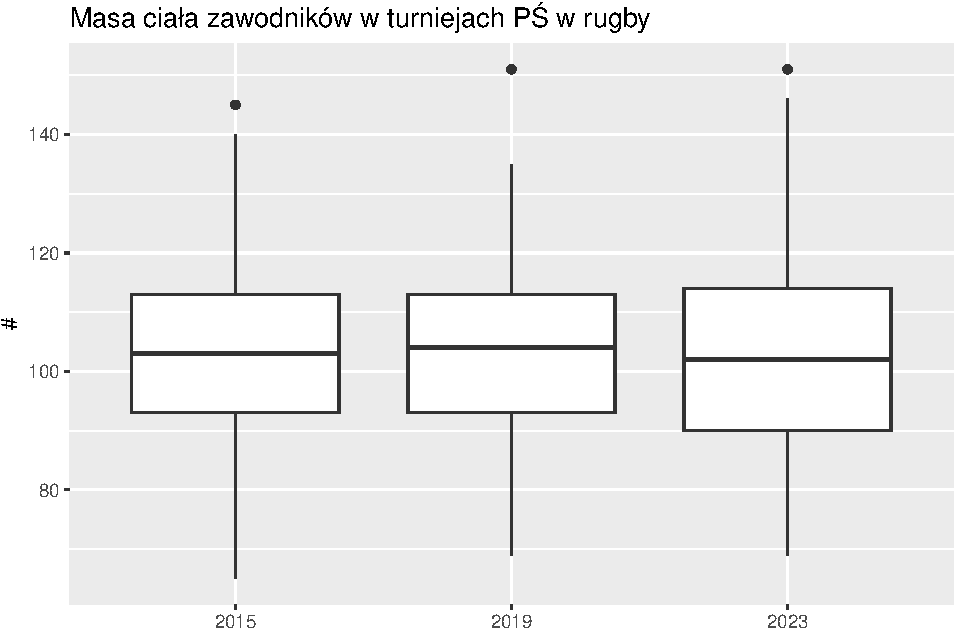
\includegraphics[width=0.9\linewidth]{_main_files/figure-latex/unnamed-chunk-21-1}
\end{example}

Od razu widać, że przeciętnie najciężsi zawodnicy byli na turnieju w roku 2019;
największe zróżnicowanie masy
ciała występowało na turnieju w roku 2023.

\hypertarget{zestawienie-metod-opisu-statystycznego}{%
\section{Zestawienie metod opisu statystycznego}\label{zestawienie-metod-opisu-statystycznego}}

W rozdziale przedstawiono osiem sposobów opisania rozkładu zmiennej:

\begin{enumerate}
\def\labelenumi{\arabic{enumi}.}
\item
  Tablice statystyczne.
\item
  Wykres słupkowy.
\item
  Wykres kołowy (niezalecany).
\item
  Histogram.
\item
  Wykres pudełkowy.
\item
  Miary tendencji centralnej: średnia, mediana, kwartyle.
\item
  Miary rozproszenia: odchylenie standardowe, rozstęp ćwiartkowy.
\item
  Miary asymetrii.
\end{enumerate}

\hypertarget{interference}{%
\chapter{Wprowadzenie do wnioskowania statystycznego}\label{interference}}

\textbf{Chcemy się dowiedzieć czegoś na temat populacji (całości)
na podstawie próby (części tej całości).}

Przykładowo chcemy ocenić ile wynosi średnia waga główki kapusty
na 100 h polu. Można ściąć wszystkie i zważyć, ale można też ściąć
trochę (pobrać próbę się mówi uczenie) zważyć i poznać średnią
na całym polu z dobrą dokładnością.

\hypertarget{masa-ciaux142a-uczestnikuxf3w-pux15b-w-rugby}{%
\section{Masa ciała uczestników PŚ w rugby}\label{masa-ciaux142a-uczestnikuxf3w-pux15b-w-rugby}}

W turnieju o Puchar Świata w rugby w 2015 roku uczestniczyło
\text{623} rugbystów. Znamy szczegółowe dane odnośnie wzrostu i wagi każdego
uczestnika turnieju. Obliczamy (prawdziwą) średnią, odchylenie standardowe
i współczynnik zmienności masy ciała:

\begin{verbatim}
##    Min. 1st Qu.  Median    Mean 3rd Qu.    Max. 
##    65,0    93,0   103,0   102,8   113,0   145,0
\end{verbatim}

Czyli średnio rugbysta na turnieju ważył
\text{102,8} kg (\texttt{Mean} na wydruku powyżej)
a odchylenie standardowe (\emph{s}) wyniosło \text{12,92} kg.

Rozkład, pokazany na rysunku \ref{fig:rwcWeight}, jest dwumodalny, bo w rugby są dwie grupy zawodników
i wcale nie wszyscy ważą ponad 110 kilogramów.

\begin{figure}
\centering
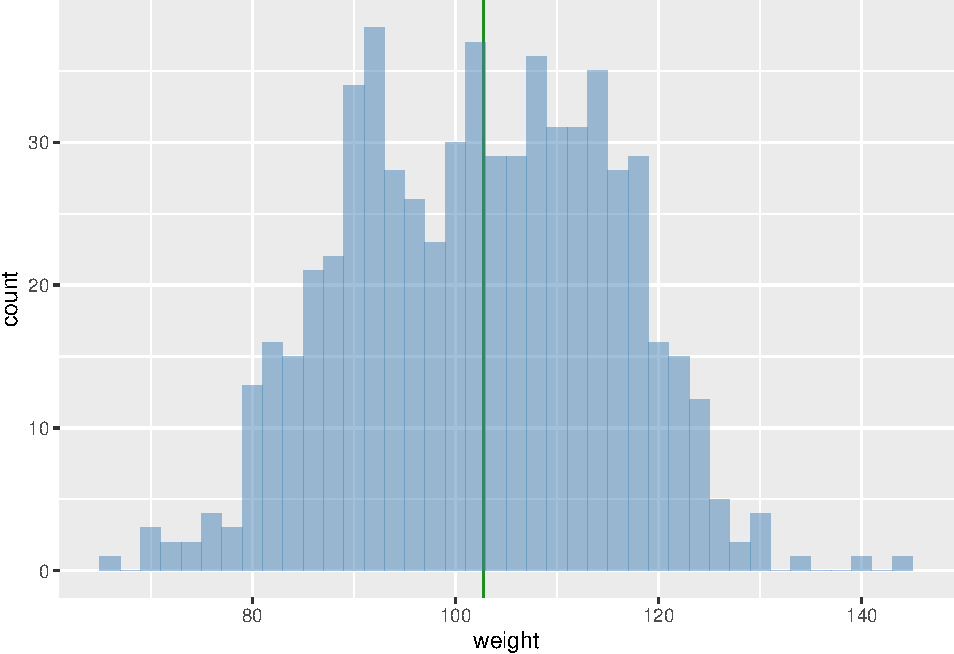
\includegraphics{_main_files/figure-latex/rwcWeight-1.pdf}
\caption{\label{fig:rwcWeight}Rozkład wagi zawodników}
\end{figure}

\textbf{Szacujemy średnią na podstawie 2 zawodników pobranych losowo}.

Powtarzamy eksperyment \text{1000} razy
(dwóch bo dla jednego nie obliczymy wariancji).

\begin{verbatim}
##    Min. 1st Qu.  Median    Mean 3rd Qu.    Max. 
##    74,0    96,5   102,5   102,4   109,0   130,0
\end{verbatim}

Średnia (średnich z próby) ma wartość \text{102,43} kilogramów
a odchylenie standardowe \text{9,2} kilogramów.
Wartość \(s/\sqrt{2}\) (odchylenie standardowe podzielone przez pierwiastek kwadratowy
z liczebności próby) jest równa \text{9,14}. Zauważmy, że ta wartość
jest zbliżona do wartości odchylenia standardowego uzyskanego
w eksperymencie (\text{9,2} vs \text{9,14}).

Zauważmy też, że wartość najniższej średniej wyniosła \text{74} kilogramów zaś najwyższej \text{130} kilogramów.
Gdybyśmy mieli pecha i wylosowali te skrajnie nieprawdziwe wartości to mylimy się
o \text{28,43} kilogramów
na minus lub \text{27,57} kilogramów na plus.

\textbf{Szacujemy średnią na podstawie 10 zawodników pobranych losowo}.

Powtarzamy eksperyment \text{1000} razy.

\begin{verbatim}
##    Min. 1st Qu.  Median    Mean 3rd Qu.    Max. 
##    90,6   100,1   103,0   102,9   106,0   114,3
\end{verbatim}

Średnia ma wartość \text{102,91} kilogramów, a odchylenie standardowe
\text{4,12} kilogramów.
Wartość \(s/\sqrt{10}\) jest równa \text{4,09}.

\textbf{Szacujemy średnią na podstawie 40 zawodników pobranych losowo}.

Uwaga: 40 zawodników to \text{6,4}\%
całości. Powtarzamy eksperyment \text{1000} razy.

\begin{verbatim}
##    Min. 1st Qu.  Median    Mean 3rd Qu.    Max. 
##    96,3   101,4   102,8   102,8   104,1   109,1
\end{verbatim}

Średnia jest równa \text{102,78} kilogramów, a odchylenie standardowe \text{2,05} kilogramów.
Wartość \(s/\sqrt{40}\) jest równa \text{2,04}.

Zauważmy też, że wartość najniższej średniej wyniosła \text{96,3} kilogramów zaś najwyższej \text{109,1282051} kilogramów.
Gdybyśmy mieli pecha i wylosowali te skrajnie nieprawdziwe wartości to mylimy się o \text{6,48} kilogramów
na minus lub \text{6,35} kilogramów na plus. Niewątpliwie wynik znacznie lepszy niż dla próby
dwuelementowej.

Podsumujmy eksperyment wykresem rozkładu wartości średnich (por. rysunek \ref{fig:wagaSrednia}).

\begin{figure}
\centering
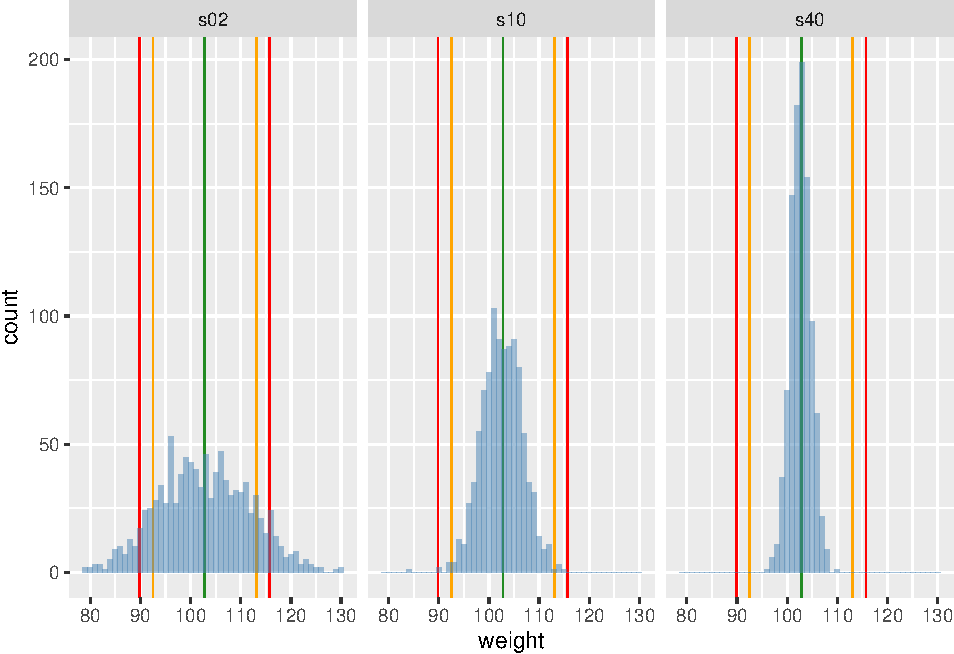
\includegraphics{_main_files/figure-latex/wagaSrednia-1.pdf}
\caption{\label{fig:wagaSrednia}Rozkład średniej wagi rugbystów w zależności od wielkości próby}
\end{figure}

\textbf{Wnioski z eksperymentu:}

Wartość średnią wyznaczamy na podstawie jakiejś konkretnej \textbf{metody}.
Wydaje się na podstawie powyższych eksperymentów, że z dobrym skutkiem
możemy jako metodę wykorzystać \textbf{średnią-z-próby}.

W ogólności taką metodą, która formalnie jest funkcją elementów z próby, nazywa się
w statystyce \textbf{estymatorem}. Warto to pojęcie zapamiętać. Wnioskujemy
o wartości nieznanego parametru w populacji posługując się estymatorem.

Kontynuując wnioski z eksperymentu należy zauważyć, że
wszystkie średnie-ze-średnich (bez względu na liczebność próby) są zbliżone do wartości
prawdziwej (to się nazywa \textbf{nieobciążoność} estymatora);
Mówiąc innymi słowy jeżeli będziemy oceniać wartość prawdziwej średniej na podstawie próby,
a naszą ocenę powtórzymy wielokrotnie,
to średnia będzie zbliżona do wartości prawdziwej (a nie np. niższa czy wyższa)
Ta cecha jest niezależna od wielkości próby.

Jeżeli rośnie liczebność próby to zmienność wartości średniej-w-próbie maleje, co za tym
idzie prawdopodobieństwo, że wartość oceniona na podstawie
średniej z próby będzie zbliżona do wartości szacowanego parametru rośnie (to się nazywa \textbf{zgodność}).
Co więcej, dobrym przybliżeniem zmienności średniej-w-próbie
jest prosta formuła \(s/\sqrt{n}\) gdzie \(n\) jest liczebnością próby a \(s\) jest odchyleniem
standardowym w populacji z której pobrano próbę.

Jeżeli mamy dwa różne estymatory służące do oszacowania parametru
i oba są \textbf{nieobciążone} oraz \textbf{zgodne}, to który wybrać?
Ten która ma \textbf{mniejszą wariancję}. Taki estymator nazywa się \textbf{efektywny}.

Estymator zatem powinien być \textbf{nieobciążony}, \textbf{zgodny} oraz \textbf{efektywny} (czyli mieć
małą wariancję). Można matematycznie udowodnić, że pewien estymator ma tak małą wariancję, że
niemożliwe jest wynalezienie czegoś jeszcze bardziej efektywnego. Takim estymatorem
średniej w populacji jest średnia z próby.

Konkretną wartość estymatora dla konkretnych wartości próby nazywamy \textbf{oceną}
(parametru).

\hypertarget{wiek-kandydatuxf3w-na-radnych}{%
\section{Wiek kandydatów na radnych}\label{wiek-kandydatuxf3w-na-radnych}}

W wyborach samorządowych w Polsce w roku 2018 o mandat radnego
sejmików wojewódzkich ubiegało się \text{7076} kandydatów.
Znamy szczegółowe dane odnośnie wieku każdego kandydata,
bo to zostało publicznie podane przez Państwową Komisję Wyborczą.
Obliczamy (prawdziwą) średnią, odchylenie standardowe
i współczynnik zmienności wieku kandydatów:

\begin{verbatim}
##    Min. 1st Qu.  Median    Mean 3rd Qu.    Max. 
##   18,00   34,00   46,00   46,24   58,00   91,00
\end{verbatim}

Czyli średnio kandydat miał \text{46,24} lat
a odchylenie standardowe wieku wyniosło \text{14,61} lat.

Rozkład znowu jest dwumodalny z jakiś powodów (por. rysunek \ref{fig:wiekKnR}).

\begin{figure}
\centering
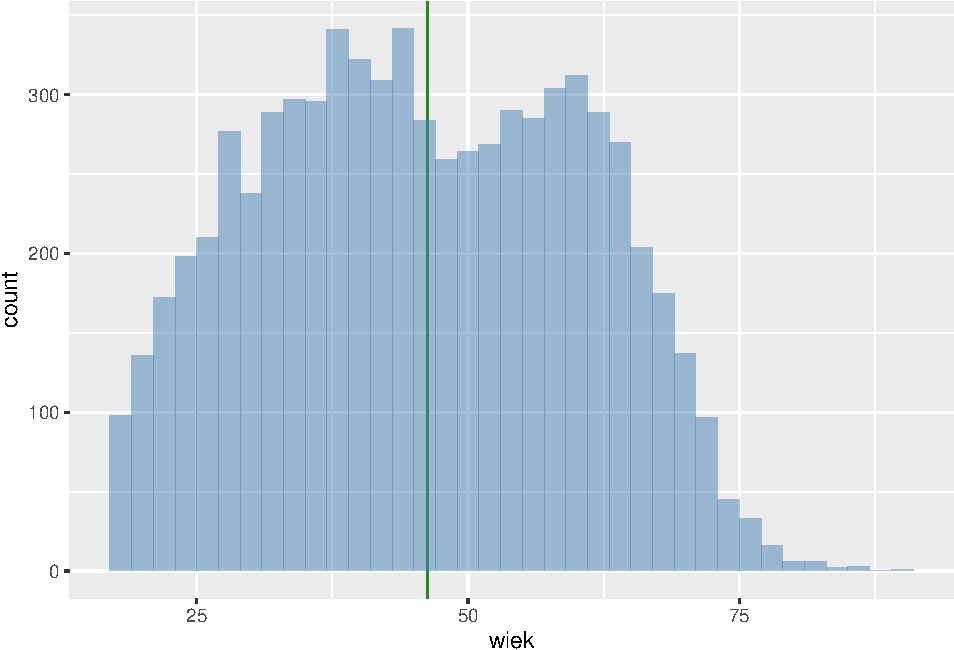
\includegraphics{_main_files/figure-latex/wiekKnR-1.pdf}
\caption{\label{fig:wiekKnR}Rozkład wieku kandydatów na radnych}
\end{figure}

\textbf{Szacujemy średnią na podstawie 2 kandydatów pobranych losowo}.

Powtarzamy eksperyment \text{1000} razy.

\begin{verbatim}
##    Min. 1st Qu.  Median    Mean 3rd Qu.    Max. 
##   18,50   38,00   45,50   45,69   52,50   75,00
\end{verbatim}

Średnia średnich z próby ma wartość \text{45,69} lat.
Odchylenie standardowe wyniosło \text{10,12}.
Wartość \(s/\sqrt{2}\) jest równa \text{10,33}.

Wartość najniższej średniej wyniosła \text{18,5} lat zaś najwyższej \text{75} lat.
Gdybyśmy mieli pecha i wylosowali te skrajnie nieprawdziwe wartości to mylimy się
o \text{27,19} lat
na minus lub \text{29,31} lat na plus.

\textbf{Szacujemy średnią na podstawie 10 kandydatów pobranych losowo}.

Powtarzamy eksperyment \text{1000} razy.

\begin{verbatim}
##    Min. 1st Qu.  Median    Mean 3rd Qu.    Max. 
##   32,20   43,30   46,40   46,28   49,30   59,40
\end{verbatim}

Średnia średnich z próby ma wartość \text{46,28} lat.
Odchylenie standardowe wyniosło \text{4,51}.
Wartość \(s/\sqrt{10}\) jest równa \text{4,62}.

\textbf{Szacujemy średnią na podstawie 40 kandydatów pobranych losowo}

Uwaga: 40 kandydatów to ok 0.6\% całości.
Powtarzamy eksperyment \text{1000} razy.

\begin{verbatim}
##    Min. 1st Qu.  Median    Mean 3rd Qu.    Max. 
##   39,33   44,80   46,33   46,28   47,77   52,02
\end{verbatim}

Średnia średnich z próby ma wartość \text{46,28} lat.
Odchylenie standardowe wyniosło \text{2,23}.
Wartość \(s/\sqrt{40}\) jest równa \text{2,31}.

\textbf{Szacujemy średnią na podstawie 70 kandydatów pobranych losowo}.

Uwaga: 70 kandydatów to około ok 1\% całości (\text{1000} powtórzeń).

\begin{verbatim}
##    Min. 1st Qu.  Median    Mean 3rd Qu.    Max. 
##   39,79   45,00   46,21   46,24   47,48   51,43
\end{verbatim}

Średnia średnich z próby ma wartość \text{46,24} lat.
Odchylenie standardowe wyniosło \text{1,74}
Wartość \(s/\sqrt{70}\) jest równa \text{1,75}.

Wartość najniższej średniej wyniosła \text{39,79} lat zaś najwyższej \text{51,43} lat.
Gdybyśmy mieli pecha i wylosowali te skrajnie nieprawdziwe wartości to mylimy się
już tylko o \text{6,46} lat
na minus lub \text{5,19} lat na plus.

Podsumujmy eksperyment wykresem rozkładu wartości średnich (rysunek \ref{fig:wiekSredni}).

\begin{figure}
\centering
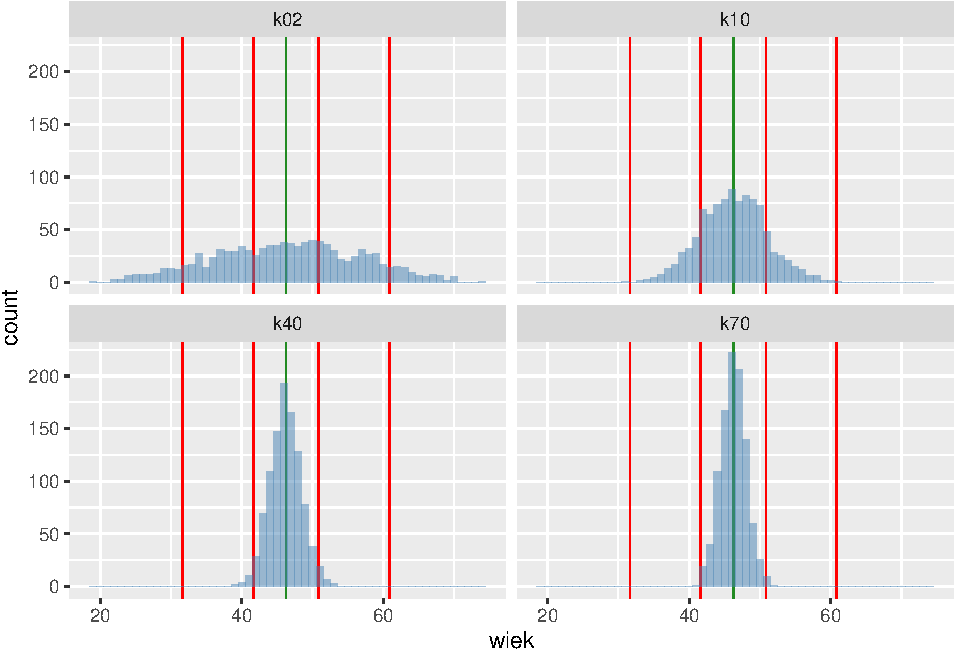
\includegraphics{_main_files/figure-latex/wiekSredni-1.pdf}
\caption{\label{fig:wiekSredni}Rozkład średniej wieku kandydatów w zależności od wielkości próby}
\end{figure}

Obserwujemy to samo zjawisko, co w przypadku wagi rugbystów: im większa próba, tym
dokładniejsza wartość średniej wieku. Bez względu na wielkość próby przeciętnie
otrzymujemy prawdziwą wartość średniej.

Wnioski:

\begin{itemize}
\item
  Precyzja wnioskowania zwiększa się wraz z liczebnością próby;
\item
  Precyzja wniskowania zwiększa się tym szybciej
  im rozproszenie w populacji generalnej jest mniejsze;
\item
  Żeby z dużą dokładnością
  wnioskować o średniej dla dużej populacji wcale nie trzeba pobierać
  dużej próby (w ostatnim przykładzie było to 1\% całości).
\end{itemize}

\hypertarget{rozkux142ad-normalny}{%
\section{Rozkład normalny}\label{rozkux142ad-normalny}}

\textbf{Rozkład empiryczny} zmiennej to
przyporządkowanie kolejnym wartościom zmiennej odpowiadających im liczebności.

Załóżmy, że istnieje zapotrzebowanie społeczne na wiedzę na temat wieku kandydatów
na radnych. Możemy to jak widać łatwo liczyć, ale jednocześnie jest to kłopotliwe.
Należy do tego mieć zbiór ponad 7 tys liczb.
\textbf{Rozkład teoretyczny} to matematyczne uogólnienie \textbf{rozkładu empirycznego}.
Jest to model matematyczny operujący pojęciem (ściśle sformalizowanym) \textbf{prawdopodobieństwa}
(zamiast liczebności). \textbf{Rozkład teoretyczny} jest:

\begin{itemize}
\item
  zbliżony do empirycznego jeżeli chodzi o wyniki (jest przybliżeniem empirycznego);
\item
  jest zdefiniowany za pomocą kilku liczb; nie ma potrzeby korzystania z liczebności.
\end{itemize}

Okazuje się, że istnieje jeden \textbf{rozkład teoretyczny}, który z dobrą dokładnością
opisuje rozkłady empiryczne będące wynikiem powyższej zabawy.
Ten rozkład (zwany \textbf{normalnym})
zależy tylko od dwóch parametrów: średniej i odchylenia standardowego, gdzie średnia będzie
równa (prawdziwej) średniej w populacji a odchylenie standardowe
równe odchyleniu standardowemu w populacji podzielonemu przez pierwiastek z wielkości próby.

Przybliżenie za pomocą rozkładu normalnego średniego rozkładu wieku kandydatów na radnych
dla próby 40- oraz 70-elementowej pokazuje rysunek \ref{fig:normalApprox}.

\begin{figure}
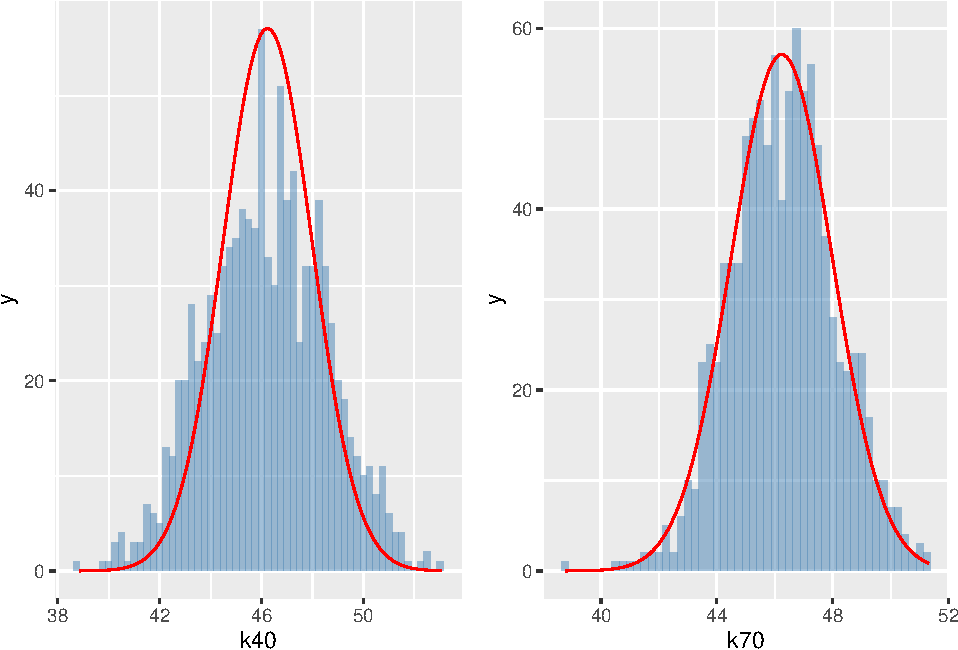
\includegraphics[width=0.99\linewidth]{_main_files/figure-latex/normalApprox-1} \caption{Rozkład normalny}\label{fig:normalApprox}
\end{figure}

Prawda, że wynik jest całkiem dobry? Teoretyczność czerwonej (w kolorowej wersji podręcznika) krzywej
polega na tym, że ona zawsze będzie identyczna, podczas gdy histogram będzie różny.
Gdybyśmy powtórzyli nasz
eksperyment (generowania \text{1000} losowych prób przypominam),
to zapewne trochę by się różnił, bo byśmy wylosowali inne wartości do prób.
Ta \textbf{teoretyczna abstrakcja} określana jest
\textbf{prawdopodobieństwem}. Rzucając monetą \text{1000} razy spodziewamy
się po \text{500} orłów i reszek,
co w modelu matematycznym będzie opisane jak:
prawdopodobieństwo wyrzucenia orła wynosi 0,5.
Rzucanie monetą to bardzo prosty eksperyment; nasz z liczeniem średniej
wieku jest bardziej skomplikowany więc miło jest się
dowiedzieć, że używając czerwonej krzywej można łatwo obliczyć jak bardzo
prawdopodobne jest na przykład popełnienie błędu większego niż 10\% średniej, albo
większego niż 0,1 lat. Albo jak duża powinna być próba żeby ten
błąd był nie większy niż 0,1 lat.

Interpretacja wartości rozkładu empirycznego zwykle jest w kategoriach ryzyka/szansy czy
prawdopodobieństwa. Przykładowo interesuje nas prawdopodobieństwo, że kandydat ma
mniej niż 30 lat.
Takich kandydatów jest \text{1091}
a wszystkich kandydatów dla przypomnienia
jest \text{7076}. Iloraz tych wartości będzie interpretowany
jako ryzyko/szansa/prawdopodobieństwo
(wynosi ono \text{15,42}\%).

Podobnie można obliczyć prawdopodobieństwo, że wiek kandydata będzie się
zawierał w przedziale 50--60 lat.
Ponieważ kandydatów w wieku 50--60 lat jest \text{1570},
to szukane prawdopodobieństwo
jest równe: \text{22,19}\%).

Jeżeli zamiast rozkładu empirycznego będziemy używać rozkład normalnego, który jak widzimy
jest jego dobrym przybliżeniem, to nie musimy liczyć empirycznych liczebności. Wystarczy że
znamy średnią i odchylenie standardowe a potrafimy obliczyć każde prawdopodobieństwo dla
każdego przedziału wartości zmiennej.

W szczególności dla rozkładu normalnego prawdopodobieństwo przyjęcia wartości z przedziału
\(m \pm s\) (średnia plus/minus odchylenie standardowe) wynosi około 0,68
prawdopodobieństwo przyjęcia wartości z przedziału \(m \pm 2 \times s\)
wynosi około 0,95 a przyjęcia wartości z przedziału \(m \pm 3 \times s\) około 0,997.
Czyli w przedziale \([-3s < m, m +3s]\) znajdują się praktycznie wszystkie wartości
rozkładu. Albo innymi słowy przyjęcie wartości spoza przedziału średnia plus/minus trzykrotność
odchylenia standardowego jest bardzo mało prawdopodobna.

Za pomocą rozkładu normalnego można opisać rozkład wagi rugbystów, wieku posłów, wagę noworodków i miliony innych rozkładów.
Uogólnieniem teoretycznym pojęcia \textbf{zmiennej statystycznej}, które do tej pory
używaliśmy jest \textbf{zmienna losowa}, tj. zmienna, która przyjmuje wartości liczbowe
z określonym prawdopodobieństwem np. określonym przez rozkład normalny.

\hypertarget{odsetek-kobiet-wux15bruxf3d-kandydatuxf3w-na-radnych}{%
\section{Odsetek kobiet wśród kandydatów na radnych}\label{odsetek-kobiet-wux15bruxf3d-kandydatuxf3w-na-radnych}}

Dane dotyczące kandydatów na radnych do sejmików wojewódzkich zawierają także płeć kandydata.
Ktoś może być ciekaw
jaki był odsetek kobiet w tej grupie. Taki parametr nazywa się proporcją
albo ryzykiem, a potocznie i niefachowo procentem.
Matematycznym modelem jest \textbf{zmienna dwuwartościowa}, która
z określonym prawdopodobieństwem przyjmuje wartość \texttt{kobieta}.
Obliczmy
empiryczną wartość tego prawdopodobieństwa jako liczbę kobiet do liczby
wszystkich kandydatów. Wartość tego parametru wynosi \text{0,4587} (albo
\text{45,87}\%).
Potraktujmy to jako prawdziwą wartość prawdopodobieństwa (p), że
kandydat jest kobietą i empirycznie sprawdźmy czy możemy szacować
o prawdziwej wartości tego parametru
używając (jako estymatora żeby się przyzwyczajać do nowych terminów) proporcji z próby.
Tradycyjnie powtarzamy eksperyment 1000 razy
dla trzech różnych wielkości próby.
Rozkład otrzymanych wartości przedstawia rysunek \ref{fig:rozkladP}.

\begin{figure}
\centering
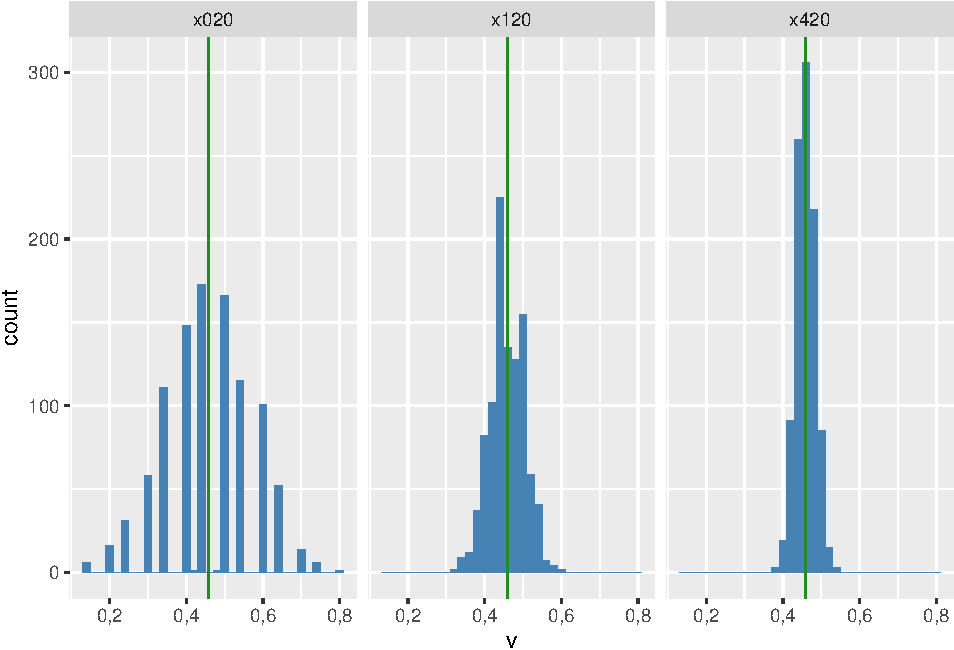
\includegraphics{_main_files/figure-latex/rozkladP-1.pdf}
\caption{\label{fig:rozkladP}Rozkład wielkości p dla różnej wielkości próby}
\end{figure}

Wnioski:

\begin{itemize}
\item
  Dla próby 20 elementowej rozkład nie przypomina rozkładu normalnego.
\item
  Dla prób 120 i 420 elementowej rozkład jest podobny do normalnego.
\item
  Zmienność estymatora maleje wraz ze wzrostem liczebności próby;
  każe nam to przypuszczać (i tak jest w istocie) że jest on zgodny.
\item
  W każdym przypadku średnia z 1000 eksperymentów jest zbliżona do wartości prawdziwej;
  każe nam to przypuszczać (i tak jest w istocie) że estymator jest nieobciążony.
\end{itemize}

Rozkład normalny jest tak magiczny że nawet jeżeli zmienna, której parametr
szacujemy nie ma rozkładu zbliżonego
do normalnego (jak w przypadku zmiennej, która przyjmuje tylko dwie wartości)
to i tak estymator tego parametru będzie normalny. Co najwyżej będziemy
potrzebowali większej próby żeby „znormalniał'' (jak w opisywanym przykładzie).

\hypertarget{wnioskowanie-statystyczne}{%
\section{Wnioskowanie statystyczne}\label{wnioskowanie-statystyczne}}

Celem analizy danych z próby jest \textbf{uogólnienie} uzyskanych wyników na całą populację. To uogólnienie
nazywa się wnioskowaniem (\emph{interferance}). Przypominamy, że \textbf{wnioskujemy}
o wartości parametru w populacji posługując się \textbf{estymatorem}. W przypadku
wnioskowania o średniej estymatorem jest średnia-z-próby.
Dobrze by było wiedzieć jak bardzo wiarygodna jest ta wartość (zwana oceną parametru) uzyskana
na podstawie konkretnego estymatora, inaczej mówiąc jak dużo mogliśmy się pomylić.

Do oceny tej wiarygodności można użyć wariancji-średniej-z-próby, która nazywa się
\textbf{wariancją błędu} (\emph{error variance}).
Jeżeli wariancja błędu jest duża, to w pojedynczej próbie mogą wystąpić wartości
znacznie różniące się od prawdziwej średniej; jeżeli jest mała to wartości bardzo różniące
się od prawdziwej średniej mają małe szanse na zaistnienie. W przypadku rozkładu
normalnego wiemy, że wariancja błędu jest równa \(s^2/n\)
(gdzie \(s^2\) jest wariancją w populacji, a \(n\) wielkością próby).

W ramach wnioskowania stosowane są trzy metody (podejścia):

\begin{itemize}
\item
  estymacja punktowa,
\item
  estymacja przedziałowa,
\item
  testowanie hipotez.
\end{itemize}

\hypertarget{estymacja-punktowa}{%
\subsection{Estymacja punktowa}\label{estymacja-punktowa}}

Szacujemy średnią (albo inny parametr) i tę wartość uznajemy za wartość prawdziwą;
dokładność szacunku jest nieokreślona. Inaczej mówiąc wartość \textbf{estymatora}
dla konkretnej próby przyjmujemy za ocenę parametru.

Estymatorem punktowym średniej jest średnia z próby a estymatorem
punktowym proporcji/ryzyka jest proporcja/ryzyko z próby.

\hypertarget{estymacja-przedziaux142owa}{%
\subsection{Estymacja przedziałowa}\label{estymacja-przedziaux142owa}}

Nie można ustalić prawdopodobieństwa popełnienia
błędu dla dokładnej wartości parametru (co wynika z właściwości matematycznych
modelu), ale można dla dowolnego przedziału od--do.

Czyli nie można ustalić, że z prawdopodobieństwem 95\%
oszacujemy wartość średnią czegoś jako 5,000000,
ale można z prawdopodobieństwem 95\% oszacować
\textbf{przedział}, w którym znajdzie się średnia (przykładowo, że będzie to przedział 4,9--5,1).

Estymacja przedziałowa to oszacowanie przedziału wartości od--do,
który z zadanym z góry prawdopodobieństwem zawiera prawdziwą wartość parametru.

Z góry wyznaczone prawdopodobieństwo nazywa się
\textbf{poziomem ufności} (określa jak często mamy się \textbf{NIE pomylić}).

\hypertarget{testowanie-hipotez}{%
\subsection{Testowanie hipotez}\label{testowanie-hipotez}}

Większość analiz statystycznych polega na porównaniu. W wyniku
tego porównania otrzymujemy liczbę. Załóżmy, że mamy dwie próby dotyczące wieku
kandydatów na radnych do sejmików wojewódzkich z roku 2018 (średnia 46,1)
oraz z roku 2014 (47,2). Różnica wynosi 1,1 lat i może być spowodowana błędem przypadkowym
(tj. gdybyśmy wylosowali jeszcze raz dwie próby, to wynik byłby zupełnie odmienny np 46,9 vs 46,5)
i/lub wynikać z tego, że faktycznie w roku 2014 kandydaci byli starsi.

Formalnie stawiamy \textbf{hipotezę}, że różnica średnich wynosi zero. Jest to tzw. \textbf{hipoteza zerowa}. Niezbędne jest także postawienie \textbf{hipotezy alternatywnej},
którą może być proste zaprzeczenie zerowej.
Zapisuje się to następująco (\(m_{14}\)/\(m_{18}\) oznacza odpowiednio średnie w latach 2014/2018):

\(H_0\): różnica średnich wieku wynosi zero (\(m_{14} = m_{18}\))

\(H_1\): różnica średnich wieku jest różna od zera (\(m_{14} \not= m_{18}\))

Hipotezy sprawdzamy wykorzystując \textbf{test statystyczny} czyli zmienną losową,
której rozkład prawdopodobieństwa zależy (jest funkcją powiedziałby matematyk)
od wartości testowanych parametrów (w tym przypadku \(m_{14}\) oraz \(m_{18}\)).
Tę zmienną losową nazywa się \textbf{statystyką testu}.

Nie jest chyba wielkim zaskoczeniem, że \textbf{statystyką testu} w teście różnicy średnich jest
różnica średnich w próbie (poprawnie mówiąc różnica uwzględniająca liczebność próby
oraz zmienność obu populacji). Całkiem \textbf{zdroworozsądkowo} możemy przyjąć, że duże wartości
\textbf{statystyki testu} świadczą na rzecz
hipotezy alternatywnej, natomiast małe na rzecz hipotezy zerowej.

Duża różnica pomiędzy \textbf{hipotezą} a wynikiem z próby może wynikać z tego, że:

\begin{enumerate}
\def\labelenumi{\arabic{enumi}.}
\item
  Pechowo trafiła nam się nietypowa próba, który zdarza się rzadko (rozkład normalny).
\item
  Hipoteza jest fałszywa, średnie mają inną wartość niż zakładamy w hipotezie zerowej.
\end{enumerate}

Statystyk zawsze wybierze drugą wersję. Pozostaje tylko ustalić co to jest rzadko (dla statystyka)?

Rzadko, to z prawdopodobieństwem mniejszym niż z góry ustalone małe prawdopodobieństwo.
zwane \textbf{poziomem istotności}. Określa ono jak często
możemy się pomylić \textbf{odrzucając hipotezę zerową, która jest prawdziwa}.

Teraz wystarczy obliczyć prawdopodobieństwo wystąpienia różnicy, którą otrzymaliśmy lub jeszcze większej
i porównać je z poziomem istotności. Jeżeli to prawdopodobieństwo jest równe lub niższe od poziomu istotności
odrzucamy hipotezę zerową (różnica jest istotna statystycznie).

Przyjmijmy przykładowo, że prawdopodobieństwo wystąpienia różnicy 1,1 lat (i większej) oszacowane
na podstawie odpowiedniego modelu matematycznego (rozkład normalny) wynosi 0,3
co znaczy że coś takiego
zdarza się względnie często -- trzy razy na 10 pobranych prób.

Załóżmy z kolei że, ta różnica wyniosła 3,2 lata. Prawdopodobieństwo
wystąpienia takiej różnicy (i większej) wynosi 0,009 co znaczy że coś takiego
zdarza się względnie rzadko -- 9 razy na tysiąc prób.

Przyjmując, że możemy się mylić 5 razy na 100 w pierwszym przypadku statystyk powie,
że nie ma podstaw do odrzucenia hipotezy \(H_0\).
Różnica 1,1 lat wynika z przypadku. W drugim wypadku
statystyk powie, że hipoteza jest fałszywa, bo zdarzyło się coś co nie powinno się zdarzyć.

Ale jest jeszcze drugi przypadek popełnienia błędu:
\textbf{przyjmujemy hipotezę zerową, która jest fałszywa}. W testach
statystycznych nie określa się prawdopodobieństwa popełnienia tego błędu, a w związku z tym nie można
\textbf{przyjąć hipotezy zerowej} (bo nie znamy ryzyka popełnienia błędu).

W konsekwencji hipotezę zerową albo się odrzuca albo \textbf{nie ma podstaw do odrzucenia}.
Wniosek cokolwiek niekonkluzywny, ale tak jest.

Dlatego też często „opłaca się'' tak postawić hipotezę zerową aby ją następnie odrzucić,
bo taki rezultat jest bardziej konkretny.

\hypertarget{testy-nieparametryczne}{%
\subsection{Testy nieparametryczne}\label{testy-nieparametryczne}}

Można testować hipotezy na temat wartości parametrów, ale można też testować
przypuszczenia o charakterze mniej konkretnym. Na przykład, że dwie zmienne
są niezależne (co to znaczy wyjaśniono w następnym rozdziale), albo
że dwa rozkłady są podobne do siebie (rozkłady nie średnie).
Takie hipotezy/testy określa się jako \textbf{nieparametryczne}.
Przykładami są testy niezależności chi-kwadrat albo normalności
Shapiro-Wilka (opisane w następnym rozdziale).

Oczywiste, ale powtórzmy: przypuszczenia o charakterze nieparametrycznym
możemy tylko testować (sprawdzać hipotezy);
nie obliczamy wtedy ani ocen ani nie wyznaczamy przedziałów ufności.

\hypertarget{statystyk-carl-pearson}{%
\section{Statystyk Carl Pearson}\label{statystyk-carl-pearson}}

W punkcie \ref{fnightingale} przypomnieliśmy postać Florence Nightingale -- matki
statystyki i bardzo dobrej kobiety. A kto był ojcem tejże statystyki?
Ojców było więcej niż matek oczywiście, a wśród nich Francis Galton (regresja),
Carl Pearson (współczynnik korelacji liniowej, test niezależności chi-kwadrat) oraz Ronald Fisher (podstawy wnioskowania).
Niestety wszyscy wymienieni byli
zadeklarowanymi rasistami oraz wyznawcami społecznego darwninizmu
i eugeniki. Pierwszymi zastosowaniami „nowoczesnych'' metod statystycznych było
naukowe udowodnienie, że biali ludzie są lepsi od innych:

\emph{Przez ile stuleci, ile tysięcy lat Kaffirowie {[}\ldots{]} lub Murzyni rządzili w Afryce
nie niepokojeni przez białych ludzi? Jednak ich walki międzyplemienne nie stworzyły cywilizacji w najmniejszym stopniu
porównywalnej z \textbf{aryjską} {[}\ldots{]}
Historia pokazuje jeden i tylko jeden sposób, w jaki powstaje wysoka cywilizacja,
a mianowicie \textbf{walka rasy} i przetrwanie rasy sprawniejszej fizycznie i psychicznie\ldots{}}

Powyższe to cytat z \emph{National Life from the standpoint of science} Carla Pearsona (Londyn 1905).

Naszym zdaniem dobrze jest pamiętać o tym fatalnym starcie „nowoczesnej statystyki'', bo chociaż
jest mało prawdopodobne, że zostanie ona znowu wykorzystania do równie odrażających celów, to
jest raczej więcej niż pewne, że będzie użyta do innych szwindli.
Jeszcze jeden argument żeby nie traktować
wyników analiz statystycznych jako wiedzy objawionej,
absolutnie pewnej i 100\% prawdziwej (por. uwagę w punkcie \ref{przedmiotS}).

\hypertarget{sux142ownik-terminuxf3w-ktuxf3re-warto-znaux107}{%
\section{Słownik terminów, które warto znać}\label{sux142ownik-terminuxf3w-ktuxf3re-warto-znaux107}}

\begin{enumerate}
\def\labelenumi{\arabic{enumi}.}
\item
  Estymacja (punktowa, przedziałowa): szacowanie wartości parametru na podstawie próby.
\item
  Estymator (nieobciążony, zgodny, efektywny): funkcja na wartościach próby która służy
  do oszacowania parametru.
\item
  Hipoteza statystyczna: przypuszczenie dotyczące parametru lub rozkładu zmiennej.
\item
  Ocena (parametru): konkretna wartość estymatora dla pewnej próby.
\item
  Poziom istotności (testu; oznaczany jako \(\alpha\); zwykle 0,05): prawdopodobieństwo popełnienia błędu.
\item
  Poziom ufności = prawdopodobieństwo, że przedział ufności zawiera prawdziwą wartość parametru;
  oznaczany jako \(1- \alpha\); zwykle 0,95.
\item
  Rozkład (prawdopodobieństwa): przypisanie prawdopodobieństwa wartościom zmiennej losowej.
\item
  Test statystyczny: metoda weryfikacji hipotezy statystycznej.
\item
  Wnioskowanie statystyczne: wnioskowanie o całości na podstawie próby.
\end{enumerate}

\hypertarget{causality}{%
\chapter{Analiza współzależności pomiędzy zmiennymi}\label{causality}}

Pomiędzy zjawiskami występują związki (zależności.) Nauki formułują te związki
w postaci \textbf{praw}. Jak takie \textbf{prawo naukowe} powstaje? Typowo w dwu etapach,
najpierw za pomocą \textbf{dedukcji} stawia się \textbf{hipotezę}, potem konfrontuje się
hipotezę z danymi (podejście hipotetyczno-dedukcyjne).
Na tym drugim etapie używa się statystyki (lub matematyki jeżeli prawo ma charakter deterministyczny).

Upraszczając \emph{metoda hypodedukcji} sprowadza się do dedukcyjnego sformułowania hipotezy, która następnie jest empirycznie \emph{falsyfikowana}, tj. próbuje się wykazać, że jest ona nieprawdziwa. Konsekwencje:
nie można dowieść prawdziwości żadnej hipotezy, można natomiast wykazać, że
hipoteza jest fałszywa.

Związki między zmiennymi mogą być albo \textbf{funkcyjne} -- wartościom jednej zmiennej
odpowiada tylko jedna wartość drugiej zmiennej lub
\textbf{stochastyczne} -- wartościom jednej zmiennej odpowiadają z pewnym
przybliżeniem wartości innej zmiennej.

Problem: czy istnieje związek (zależność) pomiędzy cechami?
Przykładowo czy istnieje związek pomiędzy paleniem (przyczyna)
a chorobą nowotworową (skutek), wiekiem a prawdopodobieństwem zgonu z powodu COVID19 itd.

Jaki jest charakter zależności? Jaka jest siła zależności?

Rodzaj konkretnej metody zastosowanej do empirycznej weryfikacji zależy
w szczególności od sposobu pomiaru danych (nominalne, porządkowe, liczbowe),
co pokazano na rysunku \ref{fig:metodyAZ}.

\begin{figure}
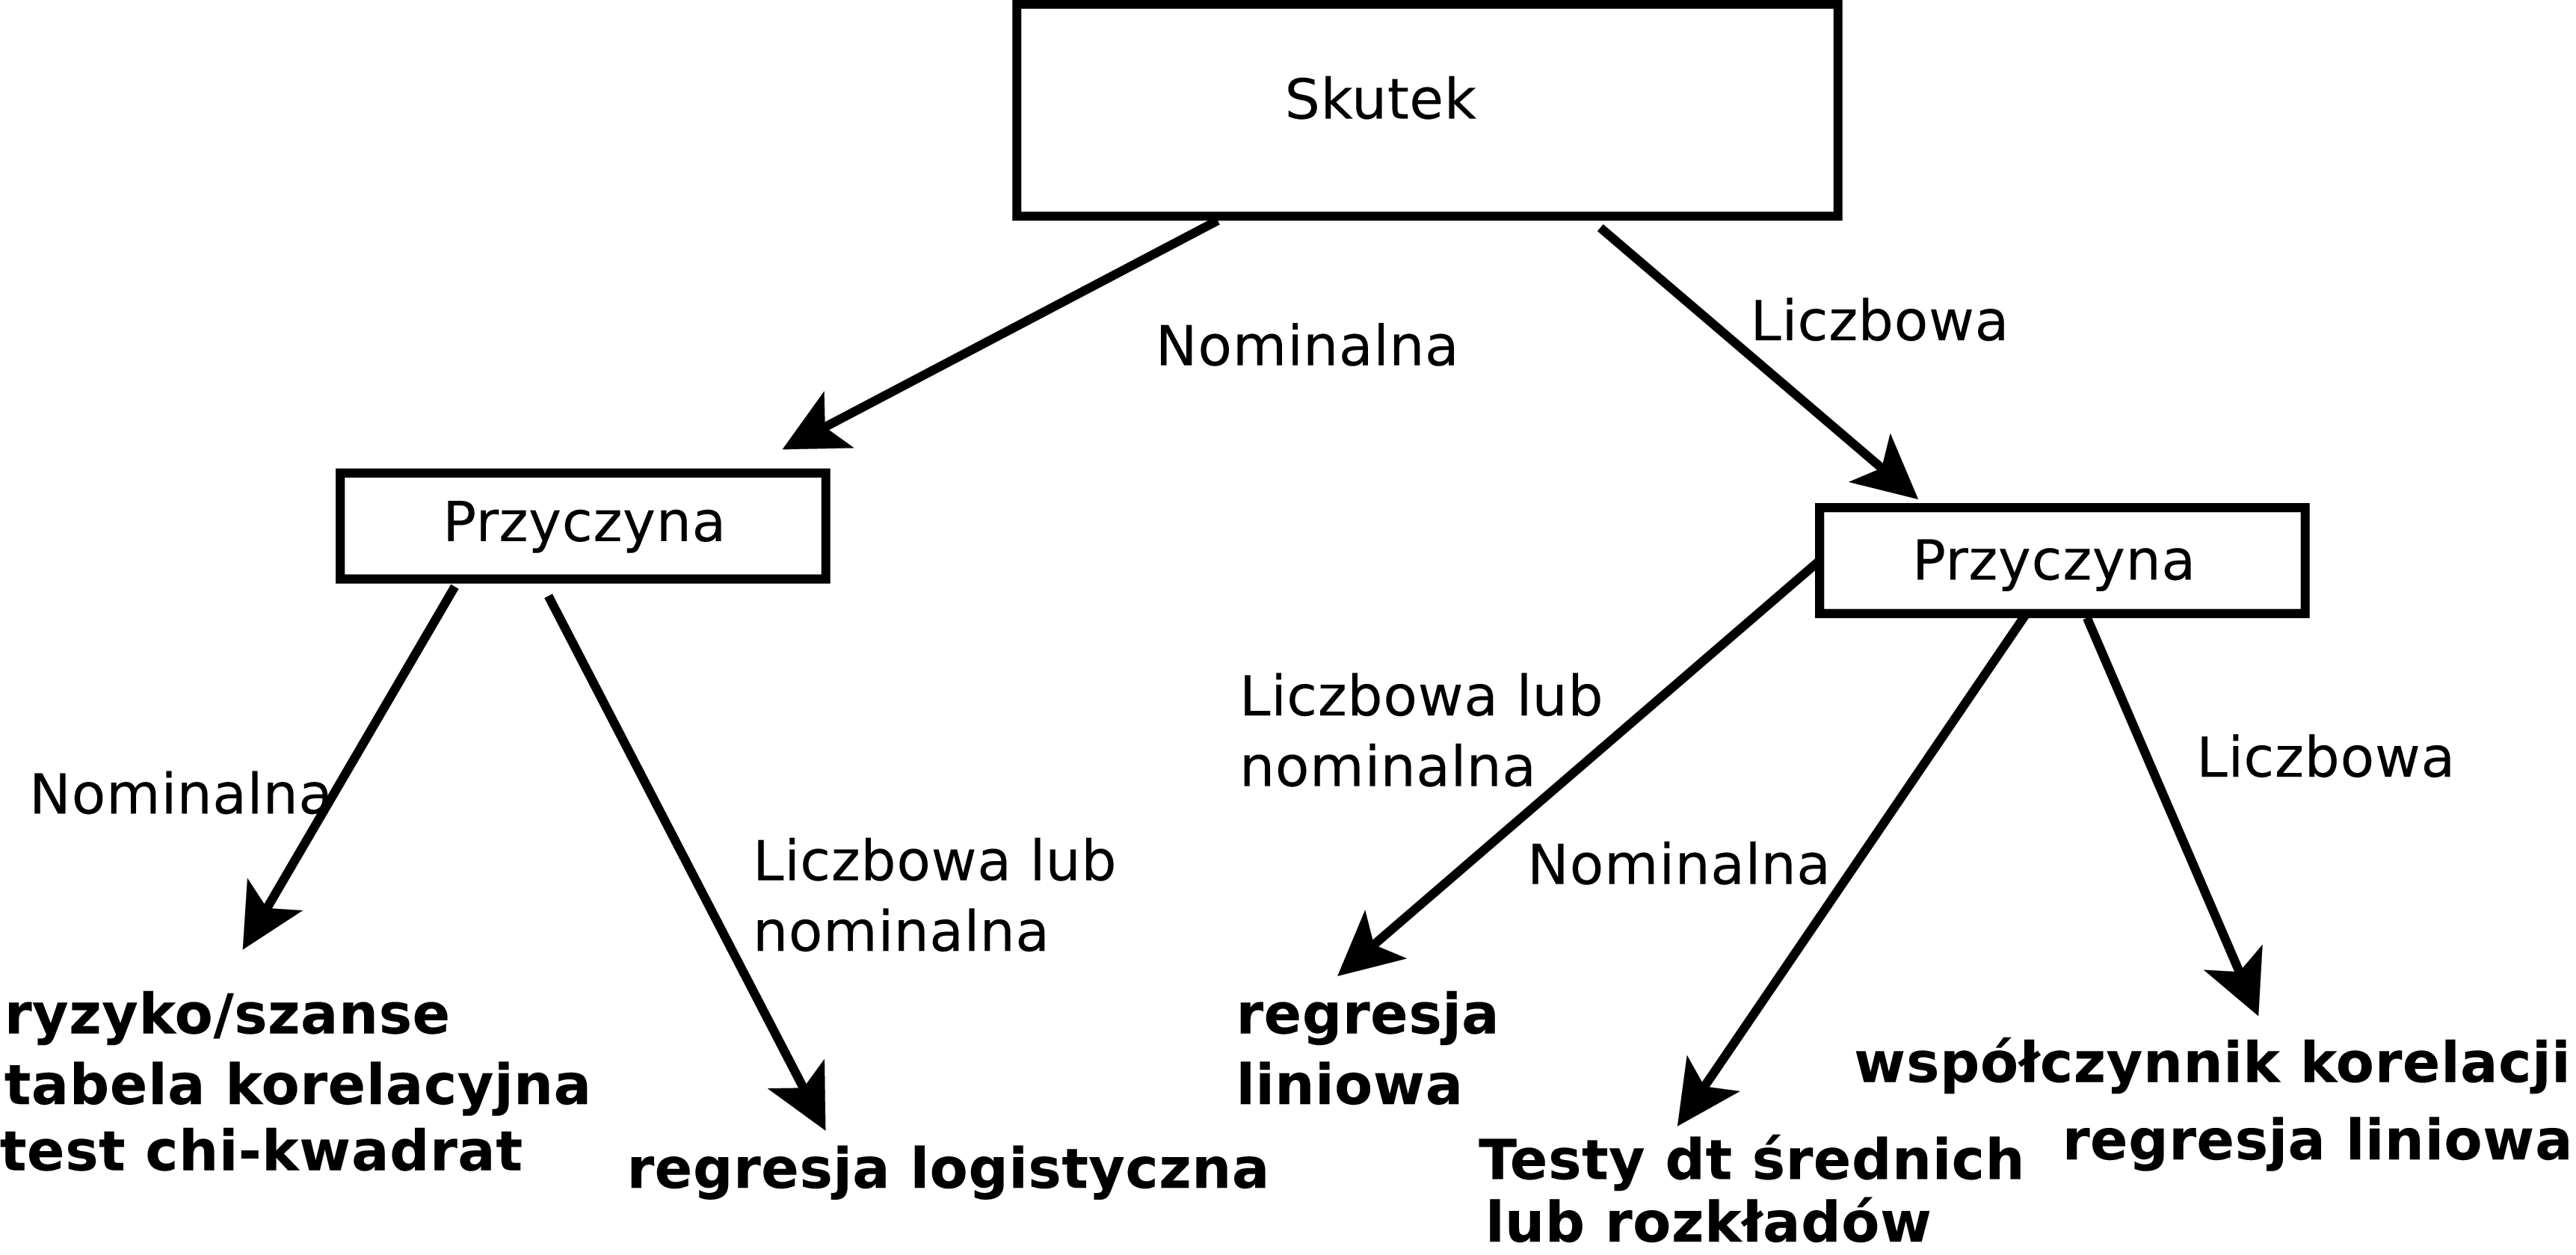
\includegraphics[width=0.99\linewidth]{./DiagramMetod} \caption{Metody statystycznej weryfikacji zależności pomiędzy zmiennymi}\label{fig:metodyAZ}
\end{figure}

Optymistyczną informacją jest, że metod (oznaczonych krojem pogrubionym na diagramie),
które omawiamy dalej w rozdziale, jest raptem siedem, czyli niedużo.

\hypertarget{dwie-zmienne-nominalne}{%
\section{Dwie zmienne nominalne}\label{dwie-zmienne-nominalne}}

\hypertarget{oddsSec}{%
\subsection{Ryzyko względne oraz iloraz szans}\label{oddsSec}}

Ryzyko to udział (iloraz) liczby sukcesów do liczby prób (zdarzeń pozytywnych/wyróżnionych do wszystkich).
Zwykle podawany w procentach. Warto zauważyć, że jest to
empiryczny odpowiednik prawdopodobieństwa.

\begin{example}
\textbf{Podawanie witaminy C a przeziębienie/brak przeziębienia}

Eksperyment, który przeprowadził Linus Pauling (laureat nagrody Nobla
za odkrycie witaminy C),
polegał na tym, że podzielił 280 narciarzy na dwie 140 osobowe grupy.
Przez 5--7 dni podawał witaminę C jednej grupie oraz placebo drugiej grupie.
Obserwował zachorowania na przeziębienie przez następne dwa tygodnie.
Jeden narciarz nie dokończył eksperymentu. Historia milczy dlaczego :-)

W grupie 139 narciarzy, którym podano witaminę C
(grupa C) zachorowało 17. W grupie 140 narciarzy, którym podano placebo (grupa P)
zachorowało 31. Zatem:

\begin{itemize}
\tightlist
\item
  Ryzyko zachorowania w grupie C wyniosło 17/139 = 12,2\%.
\item
  Ryzyko zachorowania w grupie P wyniosło 31/140 = 22,14\%.
\end{itemize}

Na tzw. chłopski rozum jeżeli witamina C \textbf{nie działa}, to powinien
zachorować ten sam odsetek narciarzy w obu grupach.
A tak nie jest jak widać.
\end{example}

Prostymi miarami oceny siły zależności mogą być:

\begin{itemize}
\tightlist
\item
  różnica ryzyk (\textbf{risk difference}),
\item
  ryzyko względne (\textbf{relative risk}), oraz
\item
  iloraz szans (\textbf{odds ratio}).
\end{itemize}

Jeżeli \(r_e\) oznacza ryzyko w grupie eksperymentalnej (\emph{test group}, grupa narażona, \emph{exposed group}),
a \(r_k\) w grupie kontrolnej (\emph{control group}, grupa nienarażona, \emph{unexposed group}),
to \textbf{różnica ryzyk} to po prostu \(r_e - r_k\).
W przykładzie będzie to \(22,14 - 12,2 = -9,94\)\%
Ta miara aczkolwiek prosta jest rzadko stosowana.

Znacznie częściej używa się \textbf{ryzyka względnego} definiowanego jako
\(RR = r_e/r_k\). Oczywiste jest, że \(RR < 1\) oznacza zmniejszenie
ryzyka; \(RR > 1\) oznacza zwiększenia; \(RR = 1\) oznacza brak zależności.

Zamiast ryzyka (czyli ilorazu liczby sukcesów do liczby prób) można używać
pojęcia szansa/szansy (\emph{odds}) definiowanego
jako iloraz sukcesów do porażek.

Jeżeli \(o_e\) oznacza szanse w grupie eksperymentalnej
a \(o_k\) w grupie kontrolnej, to \textbf{iloraz szans} (\emph{odds ratio}), jest
definiowany jako stosunek \(\textrm{OR} = o_e/o_k\).

Przykładowo jeżeli w dwukrotnym rzucie monetą otrzymano orła i reszkę to ryzyko
otrzymania orła wynosi 1/2 = 0,5 a szansa otrzymania orła wynosi 1/1 = 1.

\begin{example}
\textbf{Narciarze Paulinga (kontynuacja)}

Przypomnijmy: ryzyko zachorowania w grupie C wynosi 12,2; ryzyko zachorowania w grupie P
wyniosło 22,14. Ryzyko względne wynosi zatem \(12,2/22,14 = 0,55\).
Podanie witaminy C zmniejsza ryzyko zachorowania o prawie połowę.

Szansa, że narciarz z grupy C zachoruje wynosi 17/122 = 13,9\%.
Szansa, że narciarz w grupie P zachoruje wynosi 28,44\%.

Zatem iloraz szans
dla narciarzy wyniesie 13,9/28,44 = 0,48.
Podanie witaminy C zmniejsza szansę na zachorowanie o ponad połowę.
Albo 1/0,48 = 2,04, co oznacza, że narciarz, który nie brał witaminy C ma ponad
dwukrotnie większą szansę na zachorowanie.

Jak widać dla dużych ryzyk (rzut monetą) szansa
różni się znacznie od prawdopodobieństwa, ale dla małych ryzyk obie miary mają zbliżoną wartość.
\end{example}

Właściwości ilorazu szans:

\begin{itemize}
\tightlist
\item
  jeżeli równe 1 to sukces/porażka równie prawdopodobne;
\item
  jeżeli większe od 1 to sukces jest bardziej prawdopodobny;
\item
  jeżeli jest mniejsze od 1 to porażka jest bardziej prawdopodobna.
\end{itemize}

Dane w badaniach wykorzystujących ryzyko/szanse mają często postać
następującej tabeli dwudzielnej o wymiarach \(2\times 2\)
(a, b, c i d to liczebności):

\begin{longtable}[]{@{}lll@{}}
\toprule\noalign{}
Grupa & sukces & porażka \\
\midrule\noalign{}
\endhead
\bottomrule\noalign{}
\endlastfoot
grupa kontrolna & a & b \\
grupa eksperymentalna & c & d \\
\end{longtable}

Dla danych w tej postaci:

\begin{align}
\textrm{RR} &= (a/(a+b))/(c/(c+d))\nonumber \\
\textrm{OR} &= (ad)/(bc) \nonumber
\end{align}

\begin{example}
\textbf{Narciarze Paulinga (tabela dwudzielna)}

\begin{longtable}[]{@{}lll@{}}
\toprule\noalign{}
Grupa & katar & zdrowy \\
\midrule\noalign{}
\endhead
\bottomrule\noalign{}
\endlastfoot
grupa C & 17 & 122 \\
grupa P & 31 & 109 \\
\end{longtable}

\(\textrm{RR} = (17/(17 + 122))/(31/(31 + 109)) = 0,55\) oraz

\(\textrm{OR} = (17 * 109)/(31 * 122) =0,48\)

Otrzymaliśmy oczywiście identyczny wynik jak w poprzednim przykładzie.
\end{example}

\hypertarget{przedziaux142y-ufnoux15bci-dla-ryzyka-wzglux119dnego-i-ilorazu-szans}{%
\subsection{Przedziały ufności dla ryzyka względnego i ilorazu szans}\label{przedziaux142y-ufnoux15bci-dla-ryzyka-wzglux119dnego-i-ilorazu-szans}}

Ryzyko, ryzyko względne czy iloraz szans to parametry podobne do odsetka kobiet
wśród kandydatów na radnych z przykładu w poprzednim rozdziale. Wiemy,
że estymatorem punktowym proporcji jest proporcja z próby. Nie będzie
wielkim odkryciem, że estymatorem punktowym ryzyka jest ryzyko z próby,
ryzyka względnego/ilorazu szans zaś ryzyko względne/iloraz szans z próby.

Standardem jest obliczanie dla ryzyka względnego oraz ilorazu szans
oprócz ocen punktowych także
przedziałów ufności czyli podawania dwóch wartości, pomiędzy którymi
z zadanym prawdopodobieństwem znajduje się nieznana wartość szacowanego
parametru.

\begin{example}
\textbf{Narciarze Paulinga (przedziały ufności)}

Końce przedziałów ufności dla ilorazu szans (ocena punktowa \text{0,4899524}) wynoszą:
{[}\text{0,2569389}; \text{0,934282}{]} zaś dla
ryzyka względnego (ocena punktowa \text{0,5523323}) przedział ufności wynosi {[}\text{0,3209146}; \text{0,9506298}{]}.
\end{example}

\textbf{Uwaga}: nie jest specjalnie istotne jaka jest konkretna formuła obliczania
przedziałów ufności, przecież obliczenia i tak koniec-końców wykona
program komputerowy.

Przedział ufności dla ilorazu szans nie zawiera 1;
zatem branie witaminy C zmniejsza szanse na zachorowanie;
albo zwiększa na niezachorowanie od \(1/0,25 = 4\) do \(1/0,9 \approx 1,1\). Żeby
to zabrzmiało ładnie i po polsku: zwiększa na niezachorowanie od 10\% do 300\%.

Dlaczego taka znacząca rozpiętość? Bo próba jest względnie mała. Gdyby
Pauling zwerbował nie 280 a 2800 narciarzy mógłby weryfikować działanie
swojej witaminy z większą pewnością.

\hypertarget{tabele-wielodzielne}{%
\subsection{Tabele wielodzielne}\label{tabele-wielodzielne}}

Łączny rozkład dwóch lub większej liczby zmiennych można przedstawić
w tabeli. Taka tabela nazywa się dwudzielna (dla dwóch zmiennych)
lub wielodzielna albo wielodzielcza (dla więcej niż dwóch zmiennych).
Inne nazwy dla tabel wielodzielnych to krzyżowe albo kontyngencji
(\emph{cross-tabulation}, \emph{contingency} albo \emph{two-way tables}).

Ograniczmy się do analizy tabel dwudzielnych.

\begin{example}
\textbf{Narciarze Paulinga (kontynuacja)}

Eksperyment Paulinga można przedstawić w postaci tablicy dwudzielnej
(\texttt{P}/\texttt{C} oznacza czy narciarz zażywał witaminę czy placebo; \texttt{cold}/\texttt{nocold}
czy zachorował czy nie zachorował na katar):

\begin{tabular}{lrrr}
\toprule
  & nocold & cold & razem\\
\midrule
C & 122 & 17 & 139\\
P & 109 & 31 & 140\\
Sum & 231 & 48 & 279\\
\bottomrule
\end{tabular}

Taka tabela składa się z wierszy i kolumn. Dolny wiersz (Sum czyli Razem
po polsku) zawiera łączną liczebność dla wszystkich wierszy w danej kolumnie. Podobnie prawa skrajna kolumna zawiera łączną
liczebność dla wszystkich kolumn dla danego wiersza. Dolny wiersz/Prawą
kolumnę nazywamy \textbf{rozkładami brzegowymi}.
Pozostałe kolumny oraz wiersze nazywane
są \textbf{rozkładami warunkowymi}. Rozkładów warunkowych jest tyle ile
wynosi suma \(r + c\) gdzie \(r\) to liczba wariantów jednej cechy
a \(c\) to liczba wariantów drugiej cechy.

Przy warunku że narciarz brał witaminę C, \text{122} takich osób
nie zachorowało (\textbf{nocold}) a \text{17} zachorowało (\textbf{cold}).
Drugi rozkład warunkowy: \text{109} narciarzy, którzy brali placebo
nie zachorowało, a \text{31} zachorowało. Są także rozkłady
warunkowe dla drugiej cechy. W grupie narciarzy, którzy zachorowali
\text{122} brało witaminę C, a \text{109} brało placebo.
Wreszcie w grupie narciarzy, którzy nie zachorowali
\text{109} brało witaminę C, a \text{31} brało placebo.
Rozkładów warunkowych jest 4 bo obie cechy mają po dwa warianty. Jest
to najmniejsza możliwa tabela wielodzielna.

Zamiast liczebności można posługiwać się odsetkami (procentami):

\begin{tabular}{lrrr}
\toprule
  & nocold & cold & razem\\
\midrule
C & 43,73 & 6,09 & 49,82\\
P & 39,07 & 11,11 & 50,18\\
Sum & 82,80 & 17,20 & 100,00\\
\bottomrule
\end{tabular}

Narciarze, którzy brali witaminę C oraz nie zachorowali stanowią
\text{43,73}\%
wszystkich narciarzy. Mało przydatne\ldots{}

Ciekawsze jest obliczenie procentów każdego wiersza osobno, tj. dzielimy
liczebności w każdej kolumnie przez liczebności rozkładu brzegowego (wartości
ostatniej kolumny):

\begin{tabular}{lrrr}
\toprule
  & nocold & cold & razem\\
\midrule
C & 87,77 & 12,23 & 100\\
P & 77,86 & 22,14 & 100\\
Sum & 82,80 & 17,20 & 100\\
\bottomrule
\end{tabular}

Otrzymaliśmy ryzyka zachorowania na katar (lub nie zachorowania). Ryzyko
zachorowania dla całej grupy wynosi
\text{17,2}\% a nie zachorowania
\text{82,8}\%. Jest przyznajmy całkiem \textbf{zdroworozsądkowym założeniem}
(uczenie hipotezą statystyczną), że jeżeli przyjmowanie witaminy nie ma związku
z zachorowaniem lub nie na katar, to w grupie tych co brali i tych co nie brali
powinniśmy mieć identyczne rozkłady warunkowe równe rozkładowi brzegowemu.
Czyli powinno przykładowo zachorować
\text{17,2}\% narciarzy, którzy
brali witaminę C a widzimy , że zachorowało
jedynie \text{12,23}\%.

Na oko księgowego witamina C działa (bo są różnice), ale dla statystyka liczy się
czy ta różnica jest na tyle duża, że (z założonym prawdopodobieństwem)
można wykluczyć działanie przypadku.

Rozumowanie jest następujące: jeżeli prawdopodobieństwo wystąpienia
tak dużej różnicy jest małe, to cechy nie są niezależne.
Jest to istota i jedyny wniosek z czegoś co się nazywa
testem istotności-chi-kwadrat.
Test chi-kwadrat porównuje liczebności tablicy wielodzielnej z idealną-tablicą-wielodzielną, która zakłada niezależność jednej zmiennej od drugiej.

Można udowodnić, że taka idealna tablica powstanie przez przemnożenie dla
każdego elementu tablicy odpowiadających mu wartości brzegowych
a następnie podzieleniu tego przez łączną liczebność (czyli przykładowo pierwszy
element poniższej „idealnej'' tablicy to \text{231} pomnożone przez
\text{139} i podzielone przez \text{279}; proszę
sprawdzić,
że jest to \text{115,086}):

\begin{tabular}{lrrr}
\toprule
  & N & Y & Sum\\
\midrule
C & 115,086 & 23,914 & 139\\
P & 115,914 & 24,086 & 140\\
Sum & 231,000 & 48,000 & 279\\
\bottomrule
\end{tabular}

Proszę
zwrócić uwagę że \textbf{rozkłady brzegowe} są identyczne, identyczna
jest też łączna liczebność. Różnią się tylko rozkłady warunkowe (które nie są
liczbami całkowitymi, ale tak ma być i nie jest to błąd).

Za pomocą testu chi-kwadrat obliczamy jakie jest prawdopodobieństwo wystąpienia
tak dużych lub większych różnic. Wynosi ono \text{0,0419}.
Czyli wystąpienie tak dużych różnic
pomiędzy \textbf{oczekiwanymi} (przy założeniu o niezależności zmiennych)
a obserwowanymi liczebnościami zdarza się około 4 razy na 100.
\end{example}

Jeszcze raz przypominamy ideę testu: jeżeli prawdopodobieństwo zaobserwowanych
różnic jest małe to zakładamy że:

\begin{itemize}
\item
  albo mamy pecha i pięć razy podrzucając monetą zawsze nam spadła
  reszka (prawdopodobieństwo około 0,03), albo
\item
  że założenie co do niezależności jest fałszywe.
\end{itemize}

Statystyk zawsze wybierze
drugie. Pozostaje tylko ustalenie co to znaczy \textbf{małe}.

Małe to takie które jest mniejsze od arbitralnie przyjętego
przez statystyka. Zwykle jest to 0,05 lub 0,01 (czasami 0,1)
co oznacza że odrzucając założenie o braku związku pomiędzy
katarem a braniem witaminy C pomylimy się pięć lub raz na 100.

\textbf{Uwaga}: proszę zwrócić uwagę że wniosek z testu niezależności jest
słabszy niż z porównania ryzyk. Tam mamy informację że zależność istnieje
i oszacowaną jej wielkość (np. za pomocą ryzyka względnego) tutaj tylko
zweryfikowaliśmy fakt czy obie zmienne są niezależne lub nie.

\begin{example}
\textbf{Palenie a status społeczno-ekonomiczny}

Dla pewnej grupy osób odnotowujemy ich status-społeczno-ekonomiczny
(wysoki/\textbf{high}, średni/\textbf{middle}, niski/\textbf{low})
oraz status-względem-palenia
(wartości: pali/\textbf{current}, palił-nie-pali/\textbf{former}, nigdy-nie-palił/\textbf{never}).
Obie zmienne są nominalne, obie mają po trzy wartości. Można
poklasyfikować wszystkich badanych w następujący sposób:

\begin{tabular}{lrrrr}
\toprule
  & High & Low & Middle & Sum\\
\midrule
current & 51 & 43 & 22 & 116\\
former & 92 & 28 & 21 & 141\\
never & 68 & 22 & 9 & 99\\
Sum & 211 & 93 & 52 & 356\\
\bottomrule
\end{tabular}

Uwaga: status-społeczno-ekonomiczny to powiedzmy miara prestiżu używana w socjologii
(można na Wikipedii doczytać co to dokładnie jest).

Tym razem tabela składa się z 3 wierszy i 3 kolumn (ostatni wiersz/kolumna się
nie liczą bo to sumy -- rozkłady brzegowe).

Przedstawmy tę tabelę w postaci udziałów procentowych sumujących się
dla każdego wiersza osobno do 100\% (tj. dzielimy
liczebności w każdej kolumnie przez liczebności rozkładu brzegowego (wartości
ostatniej kolumny):

\begin{tabular}{lrrrr}
\toprule
  & High & Low & Middle & Sum\\
\midrule
current & 43,96552 & 37,06897 & 18,965517 & 100\\
former & 65,24823 & 19,85816 & 14,893617 & 100\\
never & 68,68687 & 22,22222 & 9,090909 & 100\\
Sum & 59,26966 & 26,12360 & 14,606742 & 100\\
\bottomrule
\end{tabular}

Rozumowanie jest identyczne jak dla narciarzy Paulinga. Jeżeli nie ma zależności
pomiędzy paleniem a statusem to procenty w ostatnim wierszu powinny
być identyczne jak w wierszach 1--3 (nagłówka nie liczymy). Tym idealnym
procentom odpowiadają następujące liczebności:

\begin{tabular}{lrrrr}
\toprule
  & High & Low & Middle & Sum\\
\midrule
current & 68,75281 & 30,30337 & 16,94382 & 116\\
former & 83,57022 & 36,83427 & 20,59551 & 141\\
never & 58,67697 & 25,86236 & 14,46067 & 99\\
Sum & 211,00000 & 93,00000 & 52,00000 & 356\\
\bottomrule
\end{tabular}

Wartość prawdopodobieństwa dla testu chi-kwadrat określająca, że przy założeniu niezależności obu zmiennych tak duża różnica między liczebnościami rzeczywistymi a idealnymi
(porównaj stosowne tabele wyżej) jest dziełem przypadku wynosi \text{0,001}.
Jest to prawdopodobieństwo tak małe, że statystyk odrzuca założenie o niezależności
statusu i palenia (myląc się w przybliżeniu \text{0,001} ≈ raz na tysiąc).
\end{example}

\hypertarget{zmienna-liczbowa-i-zmienna-nominalna}{%
\section{Zmienna liczbowa i zmienna nominalna}\label{zmienna-liczbowa-i-zmienna-nominalna}}

Obserwujemy wartości zmiennej liczbowej \textbf{w grupach} określonych przez wartości zmiennej nominalnej,
np. wypalenie zawodowe w podziale na miejsce pracy. Grup może być dwie lub więcej.

Stawiamy hipotezę, że wartości zmiennej w każdej grupie są równe, wobec hipotezy alternatywnej,
że tak nie jest (że są różne jeżeli grup jest dwie; co najmniej jedna jest różna jeżeli grup jest
więcej niż dwie). Stosujemy odpowiedni test statystyczny:

\begin{itemize}
\item
  jeżeli liczba grup wynosi 2 oraz można przyjąć założenie o przybliżonej
  normalności rozkładów, to stosujemy test \(t\) Welcha;
\item
  jeżeli liczba grup wynosi 2, ale nie można założyć normalności
  rozkładów, to stosujemy test U-Manna-Whitneya;
\item
  jeżeli liczba grup jest większa niż dwie oraz można przyjąć założenie
  o normalności rozkładów, to stosujemy test ANOVA z poprawką Welcha;
\item
  jeżeli liczba grup jest większa od dwóch oraz nie można przyjąć założenia
  o normalności rozkładów, to stosujemy test Kruskala-Wallisa.
\end{itemize}

Powyższe w postaci diagramu ze strzałkami przedstawiono na rysunku \ref{fig:testy}.

\begin{figure}
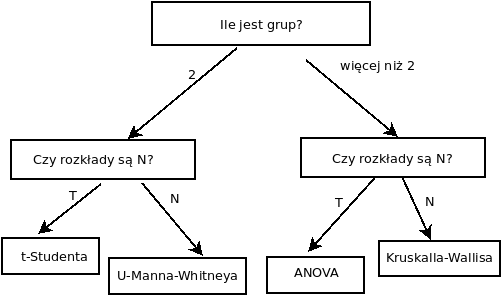
\includegraphics[width=0.8\linewidth]{./TestFlowChart} \caption{Testowanie istotności różnicy pomiędzy średnimi}\label{fig:testy}
\end{figure}

Każdy z testów jest interpretowany identycznie:

\begin{enumerate}
\def\labelenumi{\arabic{enumi}.}
\item
  Obliczana jest wartość statystyki testu \(t_k\).
\item
  Obliczane jest prawdopodobieństwo \(t \geq t_k\) czyli przyjęcia przez
  statystykę testu \(t\) równej lub większej od \(t_k\) (co do wartości bezwzględnej).
  To prawdopodobieństwo zwyczajowo oznacza się literą p albo p-value (czyli wartość p).
\item
  Jeżeli p jest mniejsze/równe od przyjętego poziomu istotności to hipotezę zerową odrzucamy;
  jeżeli p jest większe od przyjętego poziomu istotności to nie ma podstaw do odrzucenia
  hipotezy zerowej.
\end{enumerate}

Odrzucenie hipotezy zerowej oznacza, że istnieje związek pomiędzy jedną a drugą zmienną.
Jeżeli nie ma podstaw do odrzucenia
hipotezy zerowej to oznacza to że takiej zależności nie udało nam się wykazać.

Omawiając wynik należy podać się wartość \(t_k\) oraz p.~Statystyka testu może się
różnie nazywać i być oznaczana różnym symbolem,
np.: t (test t Welcha), U (test U Manna-Whitneya).

Testy \(t\) Welcha oraz ANOVA są \textbf{parametryczne}, porównujemy średnie w grupach.
Testy U-Manna-Whitneya oraz Kruskala-Wallisa są \textbf{nieparametryczne} porównujemy
rozkłady wartości zmiennej w grupach.

\hypertarget{test-t-welcha}{%
\subsection{\texorpdfstring{Test \(t\) Welcha}{Test t Welcha}}\label{test-t-welcha}}

Test stosujemy jeżeli porównujemy dwie grupy oraz można przyjąć
założenie, że rozkład wartości w obu grupach jest normalny.
Test \(t\) Welcha jest testem parametrycznym. Sprawdzamy czy średnie w grupach są równe.

\begin{example}
\textbf{Poziom depresji a miejsce pracy}

Studenci pielęgniarstwa i ratownictwa PSW w 2023 roku wypełnili
ankietę zawierającą
test depresji Becka, mierzący \textbf{poziom depresji} (wartość liczbowa)
oraz pytanie o rodzaj miejsca pracy (skala nominalna). Poniżej
zestawiono średnie wartości \textbf{poziomu depresji} w podziale
na rodzaj miejsca pracy (szpital/przychodnia).

\begin{tabular}{lrrr}
\toprule
m-pracy & średnia & mediana & n\\
\midrule
Przychodnia & 7,833333 & 7 & 12\\
Szpital & 13,252747 & 11 & 91\\
\bottomrule
\end{tabular}

Kolumna n zawiera liczebności.

Średnie różnią się
o \text{5,42}.
Pytanie czy to dużo czy mało?

Przyjmijmy (na razie bez sprawdzania), że rozkłady wartości poziomu depresji
w obu grupach są
normalne. Można zatem zastosować test \(t\) Welcha.

\begin{tabular}{llrrrr}
\toprule
Grupa1 & Grupa2 & n1 & n2 & t & p\\
\midrule
Przychodnia & Szpital & 12 & 91 & -2,895988 & 0,00978\\
\bottomrule
\end{tabular}

Kolumna t zawiera wartość statystyki testu \(t_k\). Kolumna p
zawiera oczywiście wartość prawdopodobieństwa p.

Ponieważ wartość \(p\) równa \text{0,00978} jest mniejsza od każdego zwyczajowo
przyjmowanego poziomu istotności (0,05 na przykład, albo 0,1) hipotezę, że średnie w obu grupach są równe należy odrzucić.
W konsekwencji stwierdzamy, że poziom depresji pracujących w Szpitalu
był istotnie wyższy od pracujących w Przychodni.
\end{example}

\hypertarget{testowanie-normalnoux15bci}{%
\subsection{Testowanie normalności}\label{testowanie-normalnoux15bci}}

Statystyk nie przyjmuje założeń na słowo honoru.
Kiedy zatem można przyjąć założenie o normalności a kiedy nie?
Można to ocenić na podstawie wykresu kwantylowego oraz
posługując się testem Shapiro-Wilka
(bo statystycy na każde pytanie mają zawsze \textbf{jakiś} stosowny test).

\begin{example}
\textbf{Poziom depresji a miejsce pracy}

Hipoteza zerowa w teście Shapiro-Wilka (S-W) zakłada, że rozkład cechy
jest normalny.
Interpretacja tego testu jest „standardowa``, mianowicie małe wartości \(p\)
świadczą przeciwko hipotezie zerowej.

\begin{tabular}{lrr}
\toprule
m-pracy & S-W & p\\
\midrule
Przychodnia & 0,9256178 & 0,3359655\\
Szpital & 0,8191903 & 0,0000000\\
\bottomrule
\end{tabular}

Kolumna S-W zawiera wartości statystki testu S-W oczywiście.

Rozkład w grupie \texttt{szpital} nie jest normalny (o czym świadczy niska wartość p).
Nasze założenie co do normalności
było niepoprawne i należy do weryfikacji hipotezy o równości wartości zmiennej w grupach
zamiast testu \(t\) Welcha zastosować test U Manna-Whitneya.

Wykres kwantylowy jest graficzną metodą weryfikacji normalności rozkładu
zmiennej. Dla \textbf{poziomu depresji} wygląda jak na poniższym rysunku:

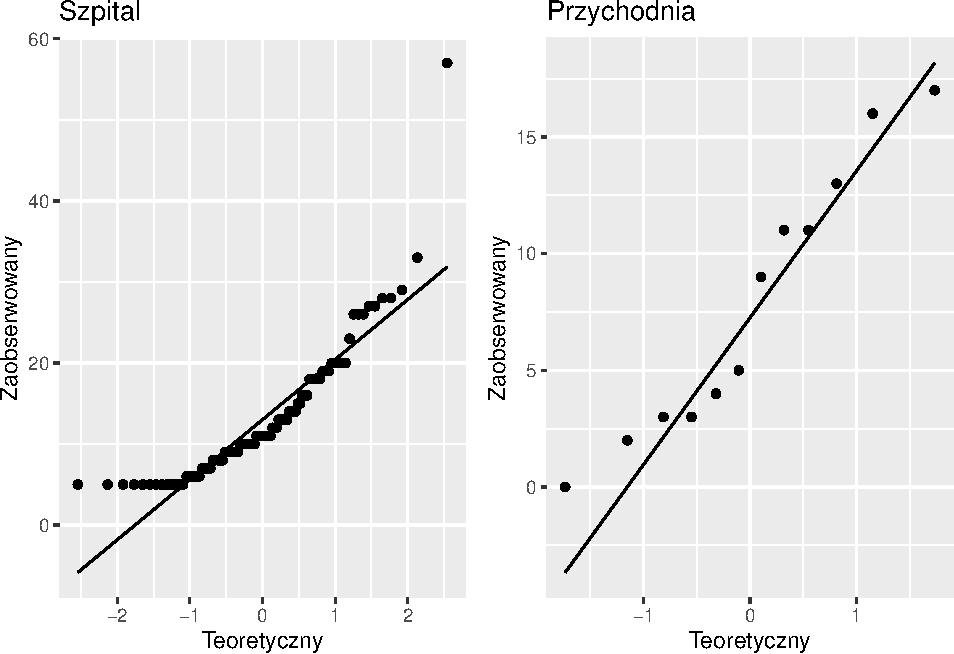
\includegraphics{_main_files/figure-latex/unnamed-chunk-45-1.pdf}

Prosta odpowiada teoretycznym wartościom kwantyli rozkładu poziomu depresji przy założeniu
że mają one rozkład normalny. Punkty odpowiadają zaobserwowanym wartościom kwantyli.
Im bardziej punkty nie pokrywają się z prostą
(zwłaszcza na skrajach rozkładu) tym mniej wierzymy, że rozkład jest normalny.

W tym przypadku wygląda, że rozkład w grupie Szpital \textbf{nie jest} normalny.
W grupie Przychodnia jest lepiej, ale jednocześnie to lepiej jest mało wiarygodne
z uwagi na małą liczebność grupy (zaledwie 12 obserwacji).
\end{example}

\hypertarget{test-u-manna-whitneya}{%
\subsection{Test U Manna-Whitneya}\label{test-u-manna-whitneya}}

Test U Manna-Whitneya jest testem nieparametrycznym. Sprawdzamy czy rozkłady
zmiennej w grupach są identyczne.

\begin{example}
\textbf{Poziom depresji a miejsce pracy}

Ponieważ grup jest dokładnie 2 a rozkład nie jest normalny, stosujemy test U Manna-Whitneya.

\begin{tabular}{llrrrr}
\toprule
Grupa1 & Grupa2 & n1 & n2 & U & p\\
\midrule
Przychodnia & Szpital & 12 & 91 & 317 & 0,0185\\
\bottomrule
\end{tabular}

Prawdopodobieństwo wystąpienia tak dużej wartości statystyki testu (U) przy założeniu, że
rozkłady zmiennej w obu grupach
są identyczne wynosi \text{0,0185}. Różnica jest zatem istotna na każdym zwyczajowo
przyjmowanym poziomie istotności (0,05 na przykład, albo 0,1); oba rozkłady różnią się.
Kolumna U zawiera wartość statystyki testu U. Przypominamy, że
dobry zwyczaj nakazuje podawać tę wartość omawiając wynik testu (więc ją podajemy).

Depresja wśród pracowników szpitali jest wyższa niż wśród pracowników
przychodni (w przypadku testu U Manna-Whitneya porównujemy wartości mediany).
\end{example}

\hypertarget{test-anova}{%
\subsection{Test ANOVA}\label{test-anova}}

Jeżeli liczba grup jest większa niż dwie, ale można przyjąć założenie
że w każdej grupie zmienna ma rozkład normalny, to stosujemy test ANOVA z poprawką Welcha.
Test ANOVA jest testem parametrycznym.
Sprawdzamy czy średnie w wszystkich grupach są równe.

\begin{example}
\textbf{Poziom depresji a staż pracy}

W ankiecie, którą wypełnili
Studenci pielęgniarstwa i ratownictwa PSW w 2023 roku
było też pytanie o staż pracy. Oryginalną liczbową wartość zmiennej
staż zamieniono na zmienną w skali nominalnej o następujących
czterech wartościach: \texttt{\textless{}6} (oznacza od 0 do 6 lat stażu pracy), \texttt{07-12} (7--12 lat), \texttt{13-18} (13--18 lat)
oraz \texttt{\textgreater{}19} (19 i więcej lat).

\begin{tabular}{lrrr}
\toprule
staż (kategoria) & średnia & mediana & n\\
\midrule
<06 & 12,84615 & 11,0 & 39\\
07-12 & 12,14286 & 9,0 & 7\\
13-18 & 10,91667 & 6,5 & 12\\
>19 & 12,95556 & 11,0 & 45\\
\bottomrule
\end{tabular}

Zakładając, że rozkłady w grupach są normalne, do weryfikacji hipotezy
o równości wszystkich średnich możemy zastosować test ANOVA z poprawką Welcha. Na poniższym wydruku kolumna F zawiera
wartość statystki testu ANOVA, a kolumna p jak zwykle wartość prawdopodobieństwa p:

\begin{verbatim}
## 
##  One-way analysis of means (not assuming equal variances)
## 
## data:  P and staz
## F = 0,14844, num df = 3,000, denom df = 20,847, p-value = 0,9295
\end{verbatim}

Wartość p równa \text{0,9295} świadczy o tym, że nie ma istotnych różnic pomiędzy średnimi, co oznacza,
że pomiędzy poziomem depresji a kategoriami stażu pracy nie ma zależności.

Czy zastosowanie testu ANOVA było poprawne? Żeby się o tym przekonać trzeba
zastosować (znowu) test Shapiro-Wilka:

\begin{tabular}{lrr}
\toprule
m-pracy & S-W & p\\
\midrule
<06 & 0,9127826 & 0,0052385\\
07-12 & 0,8939017 & 0,2956402\\
13-18 & 0,8138678 & 0,0135286\\
>19 & 0,7239373 & 0,0000001\\
\bottomrule
\end{tabular}

Wobec takiego wyniku testu do oceny istotności różnic
należy zastosować bardziej ogólny test Kruskala-Wallisa.
\end{example}

\hypertarget{test-kruskala-wallisa}{%
\subsection{Test Kruskala-Wallisa}\label{test-kruskala-wallisa}}

Test Kruskala-Wallisa jest testem nieparametrycznym. Sprawdzamy, czy rozkłady zmiennej
w grupach są identyczne.

\begin{example}
\textbf{Poziom depresji a staż pracy}

Na poniższym wydruku wartość statystyki testu jest oznaczona jako
\texttt{Kruskal-Wallis\ chi-squared} a wartość p symbolem \texttt{p-value}:

\begin{verbatim}
## 
##  Kruskal-Wallis rank sum test
## 
## data:  P by staz
## Kruskal-Wallis chi-squared = 2,6982, df = 3, p-value = 0,4405
\end{verbatim}

Prawdopodobieństwo tak dużej wartości statystyki testu
przy założeniu, że rozkłady wartości zmiennej we wszystkich grupach są identyczne wynosi
\text{0,4405} (różnice są zatem nieistotne; wszystkie rozkłady są identyczne i nie ma zależności).
\end{example}

\hypertarget{dwie-zmienne-liczbowe}{%
\section{Dwie zmienne liczbowe}\label{dwie-zmienne-liczbowe}}

\hypertarget{korelacyjny-wykres-rozrzutu}{%
\subsection{Korelacyjny wykres rozrzutu}\label{korelacyjny-wykres-rozrzutu}}

Wykres rozrzutu (\emph{scatter plot}) znany także jako korelogram, albo wykres XY,
to prosty wykres kreślony w układzie kartezjańskim, w którym każdej obserwacji
(składającej się z dwóch liczb) odpowiada kropka o współrzędnych XY.

O występowaniu związku świadczy układanie się kropek według jakiegoś
kształtu (krzywej). O braku związku
świadczy chmura punktów niepodobna do żadnej krzywej.

Punkty układające się według prostej świadczą o zależności liniowej
(wyjątek: linia pozioma lub pionowa o czym dalej) zaś
punkty układające się według krzywej świadczą
o zależności nieliniowej.

\begin{example}
\textbf{Zamożność a konsumpcja mięsa}

Organizacja Narodów Zjednoczonych do spraw Wyżywienia i Rolnictwa znana jako FAO
udostępnia dane dotyczące konsumpcji żywności
na świecie (\url{https://www.fao.org/faostat/en/\#home}). Bank światowy
udostępnia dane dotyczące dochodu narodowego (\url{https://data.worldbank.org/}).

Konsumpcja mięsa jest mierzona jako średnia konsumpcja w kilogramach w każdym kraju (\emph{per capita} się mówi);
Dochód podobnie jako średnia wielkość dochodu narodowego \emph{per capita}.
Dane dotyczą roku 2013.

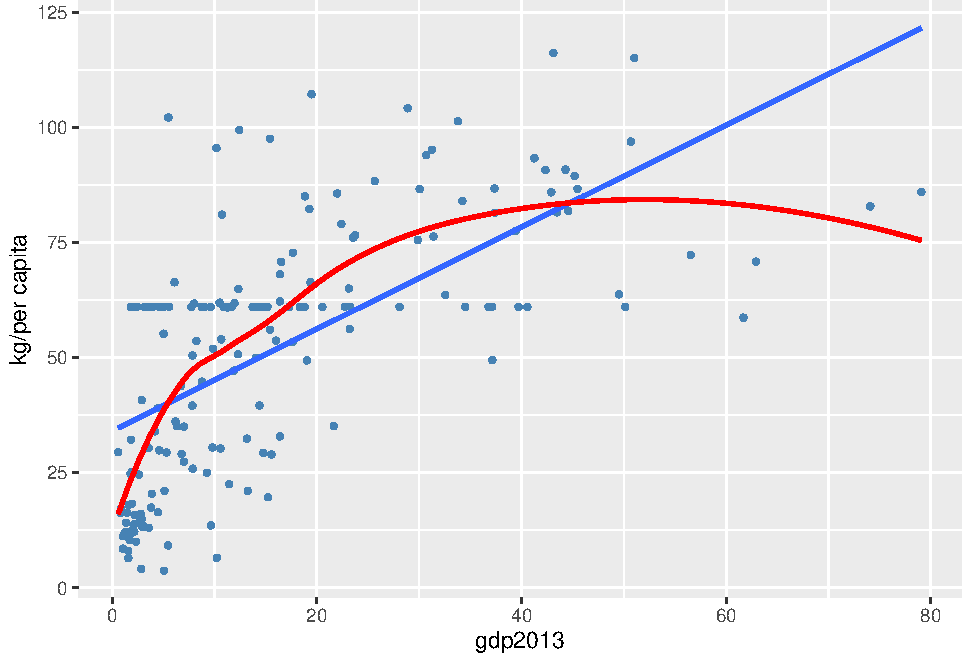
\includegraphics[width=0.9\linewidth]{_main_files/figure-latex/unnamed-chunk-51-1}

Przy dużej dozie wyobraźni można dostrzec relację liniową pomiędzy
konsumpcją mięsa a GDP co oznaczono na wykresie linią prostą. Można też założyć, że
relacja pomiędzy konsumpcją mięsa a GDP ma charakter nieliniowy (linia krzywa).
Liniowa czy nieliniowa, relacja jest na pewno mocno przybliżona co jest najbardziej
pewnym wnioskiem, który można wysnuć z wykresu rozrzutu.
\end{example}

\hypertarget{PearsonCoeff}{%
\subsection{Pomiar siły zależności: współczynnik korelacji liniowej Pearsona}\label{PearsonCoeff}}

Kowariancja to średnia arytmetyczna iloczynów odchyleń wartości zmiennych \(X\), \(Y\)
od ich wartości średnich. Dla \(n\) obserwacji na zmiennych \(X\) oraz \(Y\)
można powyższe zapisać w postaci następującej formuły:

\[\mathrm{cov} (xy) = \frac{1}{n} \left( (x_1 - \bar x) (y_1 - \bar y)  + ... +
(x_n- \bar x) (y_n - \bar y) \right)\]

Kowariancja zależy od rozproszenia (im większe tym większa),
ma też dziwną jednostkę (jednostkaX · jednostkaY) oraz zależy
od wybranych skal (tony vs gramy na przykład).

Z powyższych powodów do pomiaru związku pomiędzy cechami używa się
standaryzowanego współczynnika kowariancji,
zwanego \textbf{współczynnikiem korelacji liniowej Pearsona}, (\emph{Pearson
correlation coefficient}). Standaryzacja polega na podzieleniu wartości
kowariancji przez iloczyn odchyleń standardowych \(s_x\) oraz \(s_y\).

\[r_{xy} = \frac{\mathrm{cov}(xy) }{s_x \cdot s_y}\]

Współczynnik jest miarą niemianowaną, przyjmującą wartości ze zbioru \([-1;1]\);
Skrajne wartości \(\pm 1\)
świadczą o związku funkcyjnym (wszystkie punkty układają się na linii prostej);
wartość zero świadczy o braku związku co odpowiada linii poziomej lub pionowej
(por. rysunek \ref{fig:correlations5}).

\begin{figure}
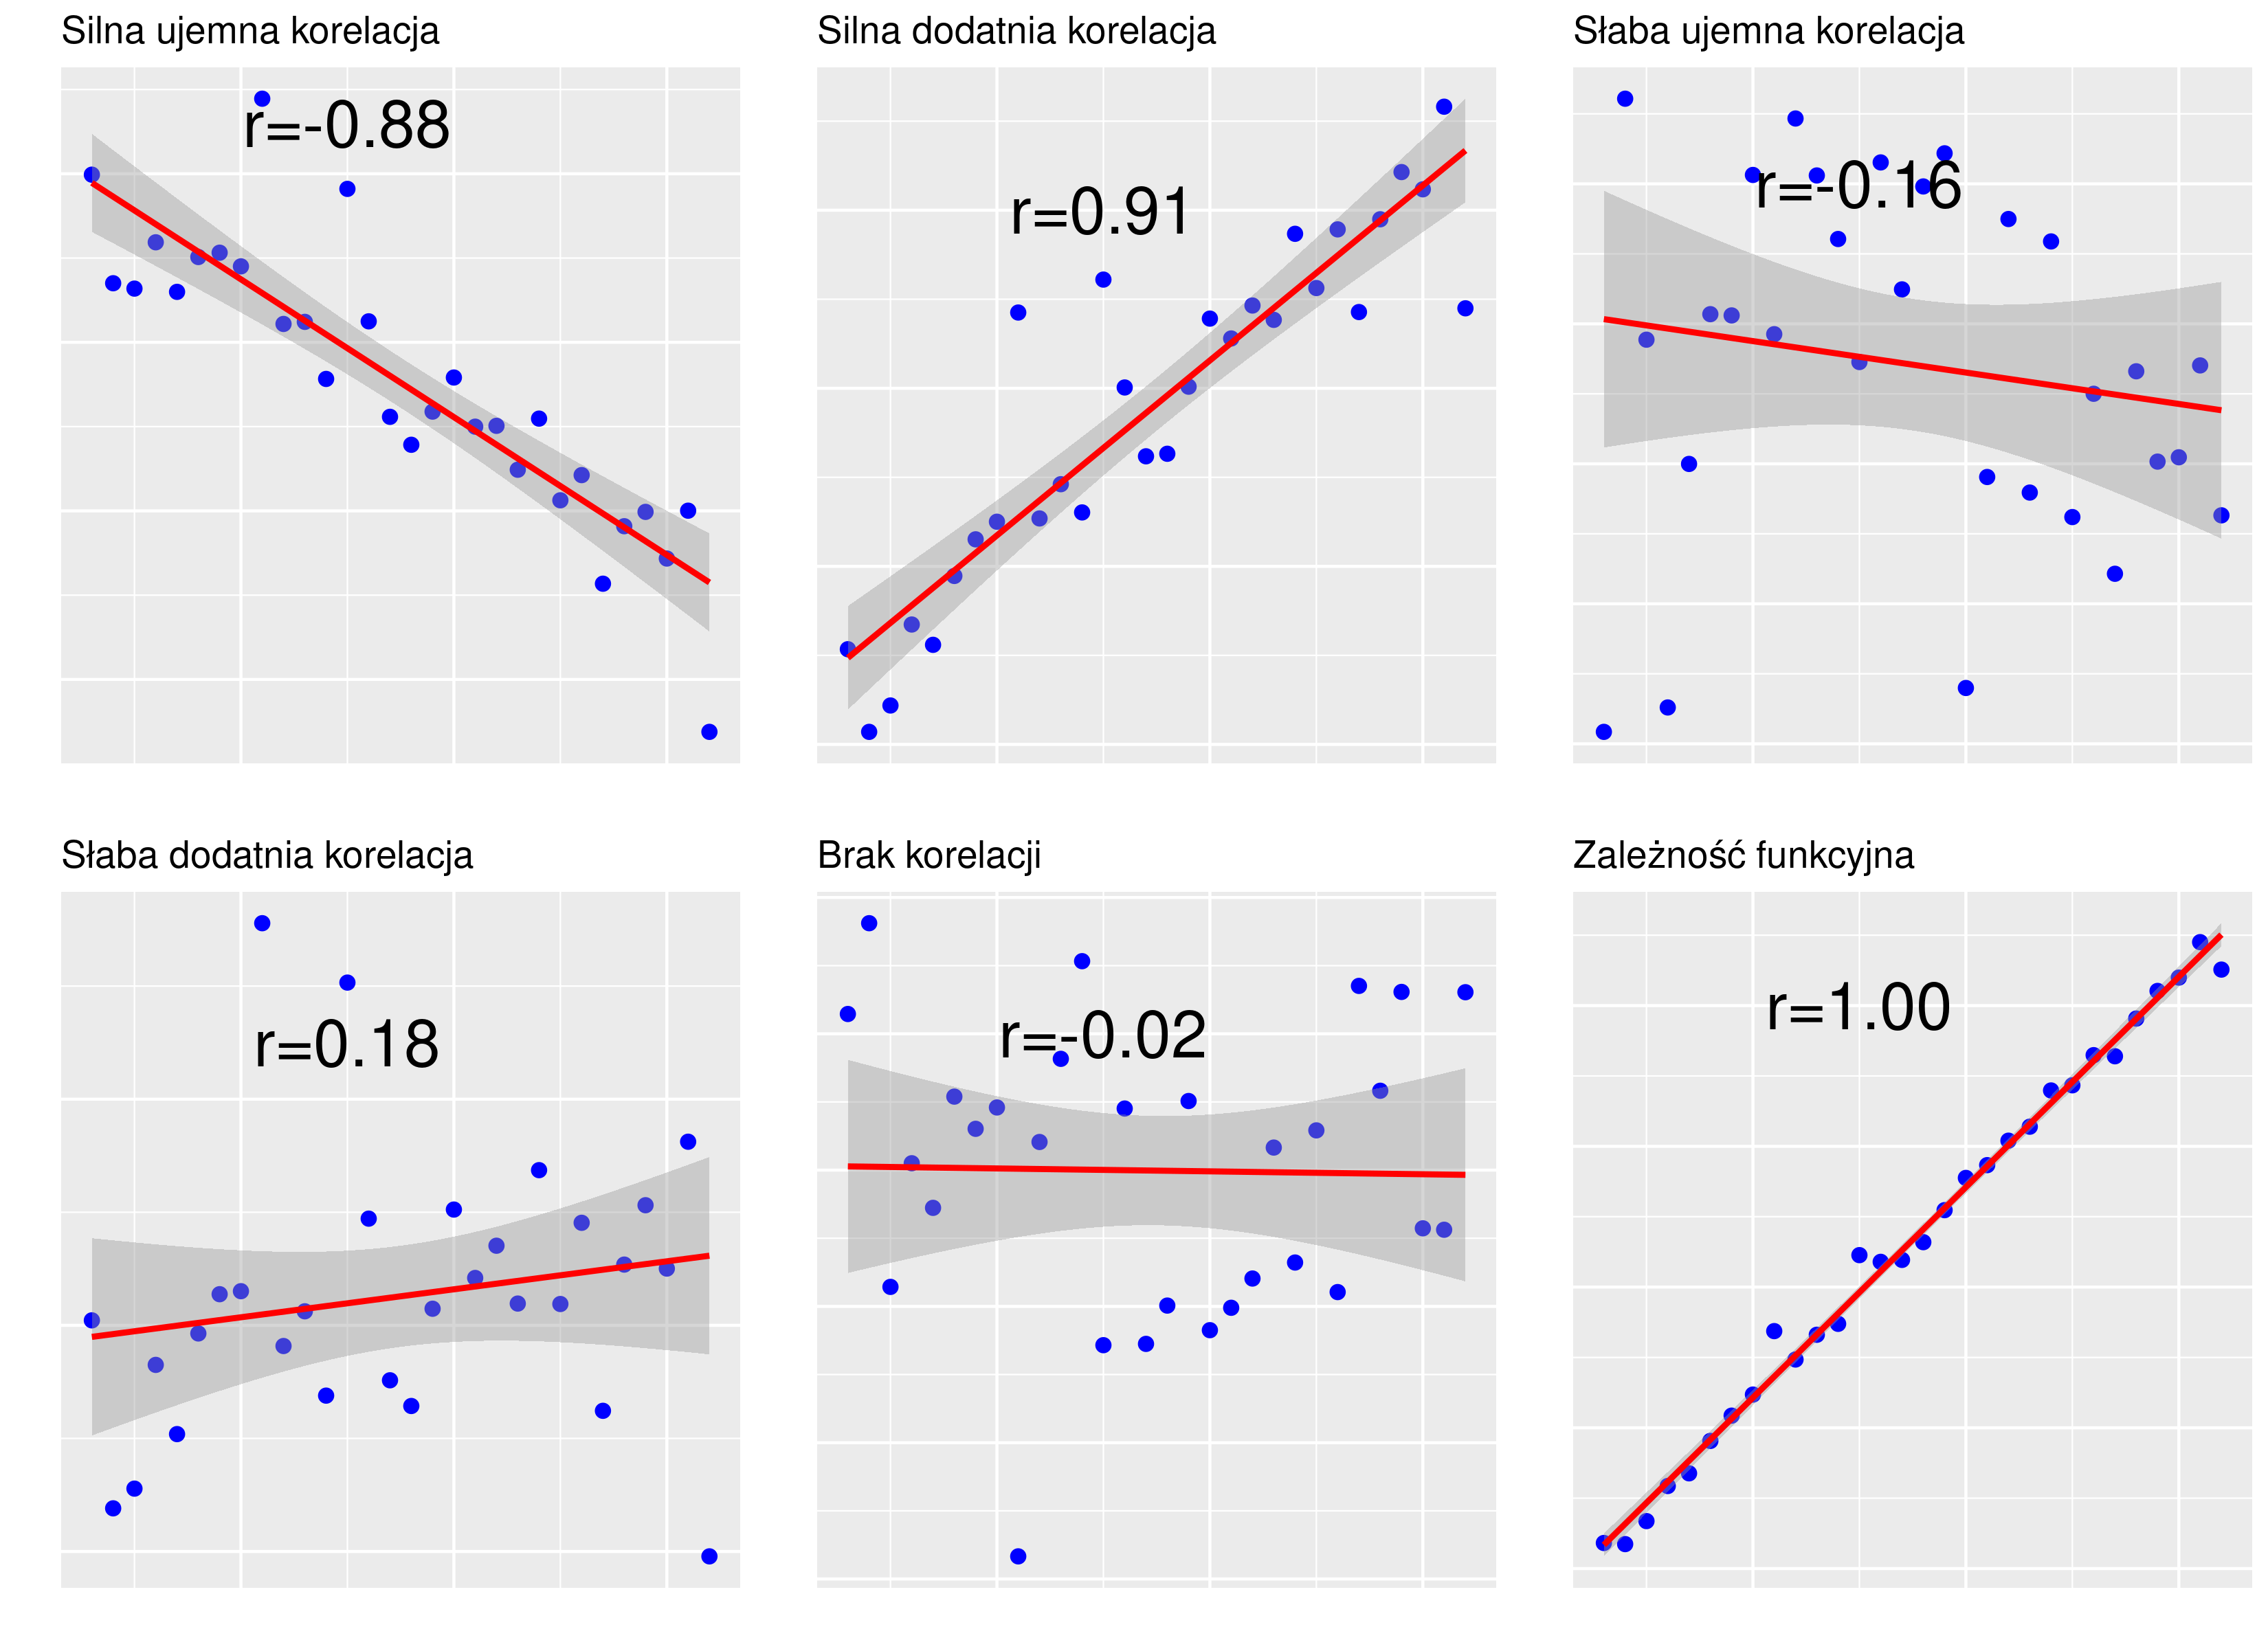
\includegraphics[width=0.99\linewidth]{./correlation_expl} \caption{Wykresy rozrzutu dla korelacji o różnej sile}\label{fig:correlations5}
\end{figure}

Interpretacja opisowa: wartości powyżej 0,9 świadczą o silnej zależności.

\begin{example}
\textbf{Zamożność a konsumpcja mięsa (kontynuacja)}

Współczynnik korelacji liniowej wynosi \text{0,6823158} (umiarkowana korelacja).

Czy ta wartość jest istotnie różna od zera? Jest na to stosowny
test statystyczny, który sprowadza się do określenia jakie jest
prawdopodobieństwo otrzymania r = \text{0,6823158} przy założeniu że
prawdziwa wartość r wynosi zero. Otóż w naszym przykładzie
to prawdopodobieństwo wynosi 3.850676e-26
(czyli jest ekstremalnie małe -- r jest istotnie różne od zera).
\end{example}

\hypertarget{macierz-korelacji}{%
\subsection{Macierz korelacji}\label{macierz-korelacji}}

Wstępnym etapem analizy zależności między zmiennymi jest często
hurtowa ocena współczynników korelacji w postaci kwadratowej \textbf{macierzy korelacji}.

\begin{example}
\textbf{Korelacja pomiędzy wiekiem, edukacją, szczęściem a stanem zdrowia}

Mohammadi S. i inni badali zależność pomiędzy wiekiem, poziomem edukacji, szczęściem a stanem zdrowia.
(The relationship between happiness and self-rated health: A population-based study of 19499 Iranian adults;
\url{https://doi.org/10.1371/journal.pone.0265914}).

\begin{verbatim}
##               age     edu Happiness Health
## age        1,0000 -0,1834    0,0449 0,0013
## edu       -0,1834  1,0000    0,0742 0,0000
## Happiness  0,0449  0,0742    1,0000 0,1786
## Health     0,0013  0,0000    0,1786 1,0000
\end{verbatim}

Albo w bardziej efektownej postaci tekstowo-graficznej:

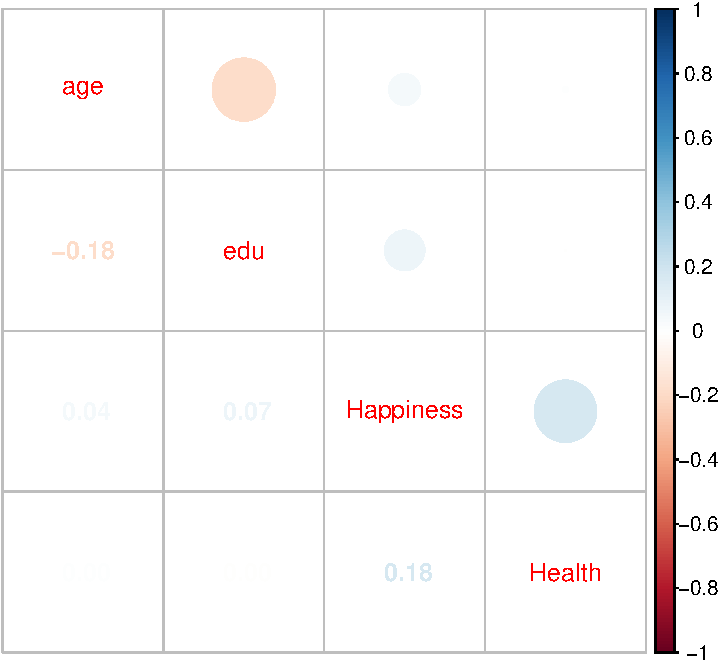
\includegraphics[width=0.75\linewidth]{_main_files/figure-latex/unnamed-chunk-54-1}

Ze wszystkich zmiennych analizowanych w badaniu Mohammadiego i innych
jedynie zależność pomiędzy wiekiem a wykształceniem
(raczej trywialna) oraz szczęściem i zdrowiem (raczej oczywista) okazały się
znacząco różne od zera.
\end{example}

\hypertarget{pomiar-siux142y-zaleux17cnoux15bci-regresja-liniowa}{%
\subsection{Pomiar siły zależności: regresja liniowa}\label{pomiar-siux142y-zaleux17cnoux15bci-regresja-liniowa}}

\textbf{Regresja liniowa} zakłada, że istnieje związek przyczyna-skutek
i ten związek można opisać linią prostą (stąd liniowa). Skutek jest
jeden i nazywa się go \textbf{zmienną zależną} a przyczyn może być wiele i noszą
nazwę \textbf{zmiennych niezależnych} (albo \textbf{predyktorów}).
W przypadku gdy związek dotyczy dwóch zmiennych mówi się o \textbf{regresji prostej}.
Przykładowo zależność
pomiędzy spożywaniem kawy w czasie sesji egzaminacyjnej a wynikiem egzaminu
można formalnie zapisać jako:

\[ \textrm{wynik} = b_0 + b_1 \cdot \textrm{kawa}\]

Współczynnik \(b_1\) określa wpływ spożycia kawy na wynik egzaminu.
W szczególności jeżeli \(b_1 = 0\) to
nie ma związku między spożywaniem kawy a wynikiem egzaminu.

\hypertarget{regProsta}{%
\subsection{Regresja prosta}\label{regProsta}}

Równanie regresji dla zmiennych \(Y\) (skutek) oraz \(X\) (przyczyna) można zapisać następująco:

\[Y = b_0 + b_1 \cdot X + e \]

\(Y = b_0 + b_1 \cdot X\) to \textbf{część deterministyczna},
a \(e\) oznacza \textbf{składnik losowy}.
O tym składniku zakładamy, że średnia jego wartość wynosi zero.
Można to sobie wyobrazić następująco: w populacji jest jakaś prawdziwa zależność
\(Y = b_0 + b_1 \cdot X\) pomiędzy \(X\) a \(Y\), która w próbie
ujawnia się z błędem o charakterze losowym. Ten błąd może wynikać
z pominięcia pewnej ważnej zmiennej (model
jest zawsze uproszczeniem rzeczywistości), przybliżonego charakteru linii
prostej jako zależności pomiędzy \(X\) a \(Y\) (prosta, ale nie do końca prosta)
albo błędu pomiaru.

Współczynnik \(b_1\) (nachylenia prostej) określa wielkość efektu
w przypadku regresji, tj. siły zależności pomiędzy zmiennymi.

Współczynnik \(b_1\) ma prostą interpretację: jeżeli wartość zmiennej \(X\)
rośnie o jednostkę to wartość zmiennej \(Y\) zmienia
się przeciętnie o~\(b_1\) jednostek zmiennej Y.
Wyraz wolny zwykle nie ma sensownej interpretacji
(formalnie jest to wartość zmiennej \(Y\) dla \(X=0\)).

Oznaczmy przez \(y_i\) wartości obserwowane (zwane też empirycznymi)
a przez \(\hat y_i\) \emph{wartości teoretyczne} (leżące na prostej linii regresji).

Wartości \(b_0\) oraz \(b_1\) wyznacza się minimalizując sumę kwadratów
odchyleń wartości teoretycznych od wartości empirycznych, tj.:

\[(\hat y_1 - y_1)^2 + (\hat y_2 - y_2)^2 + ... +  (\hat y_n - y_n)^2 \to \min\]

Rozwiązując powyższy \textbf{problem minimalizacyjny} otrzymujemy wzory
określające wartości parametrów \(b_0\) oraz \(b_1\). Metoda wyznaczania parametrów
linii prostej w oparciu o minimalizację sumy kwadratów odchyleń
nosi nazwę \textbf{metoda najmniejszych kwadratów}.

Przypominamy, że \textbf{estymatorem} nazywamy metodę oszacowania parametru na podstawie próby.
Ponieważ traktujemy \(b_0\) oraz \(b_1\) jako parametry pewnej populacji generalnej
to „wzory na \(b_0\) oraz \(b_1\)`` statystyk nazwie estymatorami parametrów \(b_0\) oraz \(b_1\).

Przypominamy dalej, że wartość średnia \textbf{dobrego estymatora} powinna wynosić zero (bo wtedy nie ma błędu systematycznego),
oraz że wariancja estymatora powinna maleć wraz ze wzrostem liczebności próby. Można udowodnić
że estymatory parametrów \(b_0\) oraz \(b_1\)
uzyskane \textbf{metodą najmniejszych kwadratów} posiadają obie właściwości.

Graficznie \textbf{kryterium minimalizacyjne} przedstawia rysunek \ref{fig:KMNK}.

\begin{figure}
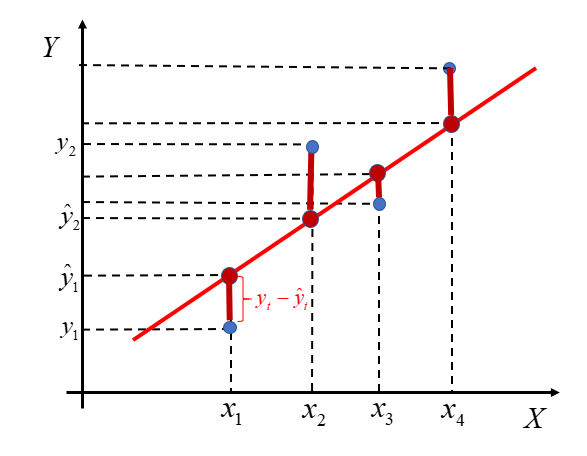
\includegraphics[width=0.8\linewidth]{./kmnk_roznice} \caption{Metoda najmniejszych kwadratów}\label{fig:KMNK}
\end{figure}

Suma podniesionych do kwadratu odległości pomiędzy czerwonymi
(leżącymi na linii prostej w wersji czarno-białej)
i niebieskimi kropkami ma być minimalna. Kropki niebieskie to
wartości empiryczne; kropki czerwone to wartości teoretyczne.
Zadanie wyznaczenie
parametrów takiej prostej oczywiście realizuje program komputerowy.

Można udowodnić, że bez względu czy punkty na wykresie układają się
w przybliżeniu wzdłuż prostej czy nie, zawsze \textbf{jakaś prosta} zostanie
dopasowana (jeżeli tylko punktów jest więcej niż jeden).
Jak ocenić w sposób bardziej konkretny, a nie tylko na oko jakość dopasowania
prostej do wartości empirycznych?

\textbf{Ocena dopasowania: wariancja resztowa oraz średni błąd szacunku}

Oznaczając \emph{resztę} jako: \(e_i = y_i - \hat y_i\), definiujemy \textbf{wariancję
resztową} jako:

\[s_e^2 = \frac{e_1^2 + e_2^2 + ... e_n^2}{n-k}\].

Gdzie \(n\) oznacza liczbę obserwacji (liczebność próby), a \(k\) liczbę
szacowanych parametrów bez wyrazu wolnego czyli jeden w regresji
prostej (a więcej niż jeden w regresji wielorakiej o czym dalej).

Pierwiastek kwadratowy z \textbf{wariancji resztowej}
nazywamy \textbf{średnim błędem szacunku} (\emph{mean square error}, MSE).

\textbf{Ocena dopasowania: współczynniki zbieżności i determinacji}

Suma kwadratów reszt (albo odchyleń wartości teoretycznych
od wartości empirycznych,
albo suma kwadratów błędów vel \textbf{resztowa suma kwadratów}):

\[\mathrm{RSK} = (y_1 - \hat y_1)^2 + (y_2 - \hat y_2)^2 + ... +  (y_n - \hat y_n)^2\].

Suma kwadratów odchyleń \textbf{wartości empirycznych}
od średniej (\textbf{ogólna suma kwadratów}):

\[\mathrm{OSK} = (y_1 - \bar y)^2 + (y_2 - \bar y)^2 + ... +  (y_n - \bar y)^2\]

Suma kwadratów odchyleń \textbf{wartości teoretycznych}
od średniej (\textbf{wyjaśniona suma kwadratów}):

\[\mathrm{WSK} = (\hat y_1 - \bar y)^2 + (\hat y_2 - \bar y)^2 + ... +  (\hat y_n - \bar y)^2\]

Można wykazać, że \(\mathrm{OSK} = \mathrm{WSK} + \mathrm{RSK}\) zatem (po podzieleniu obu stron
równania przez \(\mathrm{OSK}\)) otrzymujemy:

\[ 1 =  \mathrm{WSK}/\mathrm{OSK} + \mathrm{RSK}/\mathrm{OSK}\]

\textbf{Współczynnik zbieżności} oznaczany jako \(R^2\) to \(\mathrm{WSK}/\mathrm{OSK}\).

\textbf{Współczynnik determinacji} oznaczany jako \(\Phi^2\) (duża grecka litera Fi) to \(\mathrm{RSK}/\mathrm{OSK}\).

Współczynniki przyjmują wartość z przedziału \([0,1]\) lub \([0, 100]\)\% jeżeli
ich wartości zostaną pomnożone przez 100.

Interpretacja współczynnika zbieżności: udział (procent) zmienności wyjaśnianej
przez linię regresji. Im \(R^2\) jest bliższe jedności (lub 100\% jeżeli
jest współczynnik zbieżności jest wyrażony w procentach) tym lepiej.

\textbf{Ocena dopasowania: istotność parametru \(b_1\)}

Jeżeli: \(Y= 0 \cdot X + b_0\), to \(Y = b_0\) czyli nie ma zależności
pomiędzy \(X\) oraz \(Y\).
Wartości \(b_1\) bliskie zero wskazują na słabą zależność
pomiędzy cechami.

Przypominamy, że \textbf{estymator} parametru \(b_1\) ma średnią równą prawdziwej wartości \(b_1\).
Dodatkowo zakładamy, że rozkład tego estymatora jest normalny, co
pozwala wiarygodnie oszacować jego wariancję.
W konsekwencji znamy jego dokładny rozkład, bo przypominamy, że rozkład
normalny jest określony przez dwa parametry: średnią oraz wariancję (lub
odchylenie standardowe).

Można teraz zadać pytanie jeżeli faktycznie \(b_1=0\), to jakie jest prawdopodobieństwo, że
współczynnik \(\hat b_1\) oszacowany
na podstawie \(n\) obserwacji będzie (co do wartości bezwzględnej) większy niż \(b_e\).
Albo inaczej: otrzymaliśmy \(b_e\), jakie jest prawdopodobieństwo
otrzymania takiej wartości (lub większej co do wartości bezwzględnej)
przy założeniu, że istotnie \(b_1=0\).

Jeżeli takie prawdopodobieństwo jest duże, to uznajemy, że \(b_1 = 0\),
a jeżeli małe, to będziemy raczej sądzić, że \(b_1 \not= 0\).
Duże/małe przyjmujemy arbitralnie, zwykle
jest to \(0,1\), \(0,05\) lub \(0,01\). To prawdopodobieństwo
to oczywiście poziom istotności.

W każdym programie komputerowym na wydruku wyników linii regresji są podane wartości
prawdopodobieństwa \(b_1 > b_e\) (co do wartości bezwzględnej). Jeżeli jest
ono mniejsze
niż ustalony \textbf{poziom istotności} to \(b_1\) ma wartość istotnie różną od zera.
Oprócz wartości prawdopodobieństwa drukowana jest także wartość
błędu standardowego parametru zwykle oznaczana jako \texttt{SE} (\emph{standard error}). Wartość
\texttt{SE} nie jest wprawdzie potrzebna do oceny istotności (wystarczy prawdopodobieństwo), ale
dobry zwyczaj nakazuje podawać także tę wartość w raporcie.

Testowanie istotności współczynnika regresji jest ważnym kryterium oceny
jakości dopasowania.
Regresja z \textbf{nieistotnym} współczynnikiem nie
może być podstawą do interpretowania zależności pomiędzy \(X\) oraz \(Y\).

\begin{example}
\textbf{Waga a wzrost rugbystów}

Zależność między wagą (\texttt{weight}) a wzrostem (\texttt{height}):

\[ \textrm{height} = b_0 + b_1 \textrm{weight}\]
Oszacowanie tego równania na próbie \text{635} uczestników
Pucharu Świata w rugby w 2023 roku
daje następujące wyniki:

\begin{tabular}{lrrrrl}
\toprule
Zmienna & B & SE & z & p & CI95\\
\midrule
(Intercept) & 155,926 & 1,753 & 88,969 & 0 & 152,48 159,37\\
weight & 0,294 & 0,017 & 17,305 & 0 & 0,26   0,33\\
\bottomrule
\end{tabular}

Pierwsza kolumna \texttt{Zmienna} zawiera nazwy zmiennych (\texttt{(Intercept)} oznacza wyraz wolny).
Druga kolumna oznaczona jako \texttt{B} zawiera oszacowane wartości (oceny) parametrów linii regresji.
Kolumna \texttt{SE} zawiera oceny błędu standardowego estymatorów parametrów linii regresji.
Kolumna \texttt{p} zawiera prawdopodobieństwo \(b>b_e\).

Wzrost wagi zawodnika o 1kg
skutkuje przeciętnie większym wzrostem o \text{0,294} cm. Współczynnik determinacji
wynosi \text{32,86}\%.
Współczynnik nachylenia prostej jest istotny ponieważ wartość \(p\) (tak mała, że w tabeli
oznaczona jako 0)
jest grubo poniżej zwyczajowego poziomu istotności (p \textless{} 0,05).

Kolumna \texttt{CI95} zawiera 95\% przedziały ufności: z 95\% prawdopodobieństwem wartość współczynnika nachylenia
prostej znajduje się w przedziale 0.260--0.330.

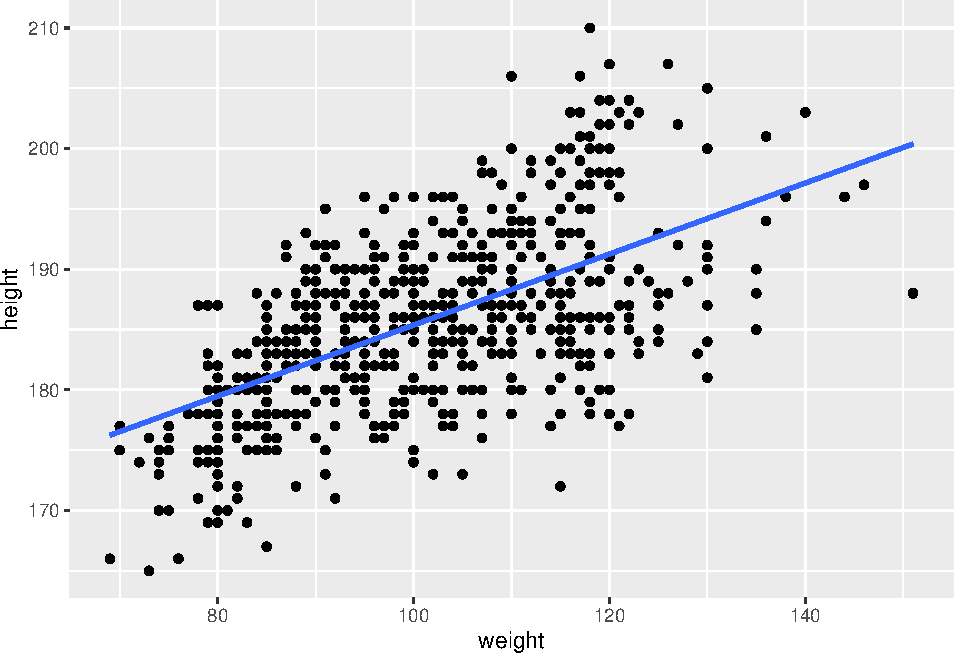
\includegraphics[width=0.75\linewidth]{_main_files/figure-latex/unnamed-chunk-57-1}
\end{example}

\begin{example}
\textbf{Zamożność a konsumpcja mięsa}

Następujący równanie opisuje zależność pomiędzy dochodem narodowym na głowę (tys USD \emph{per capita})
a konsumpcją mięsa w kilogramach:

\[\textrm{konsumpcja} = b_0 + b_1 \textrm{gdp}\]

Model oszacowano dla krajów świata w roku 2013 na podstawie danych
pobranych z bazy FAO Food Balance Sheet oraz Banku Światowego, otrzymując
następujące wyniki:

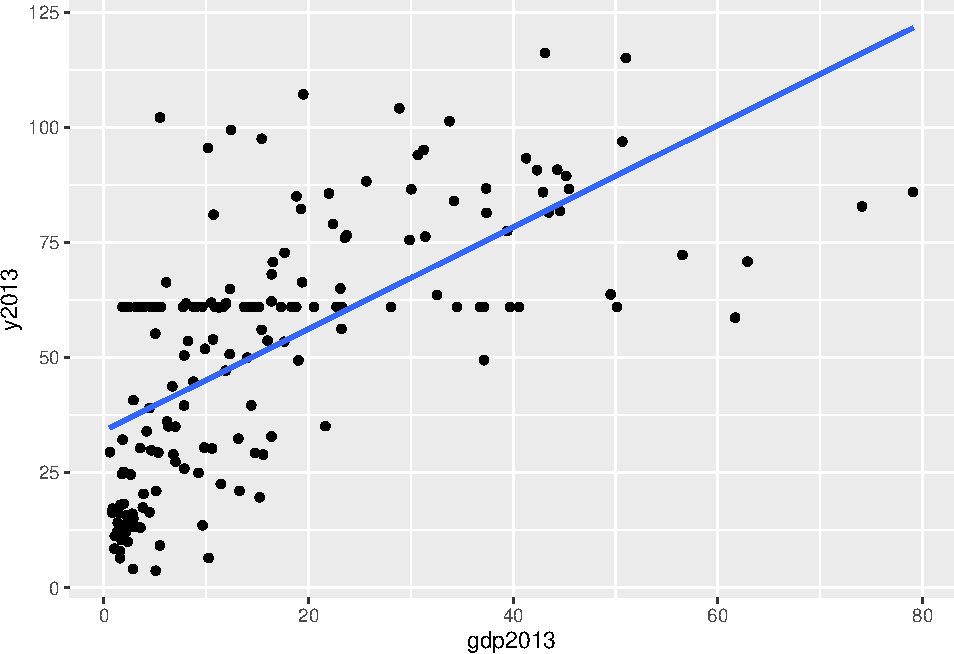
\includegraphics[width=0.75\linewidth]{_main_files/figure-latex/unnamed-chunk-59-1}

\begin{tabular}{lrrrrl}
\toprule
Zmienna & B & SE & z & p & CI95\\
\midrule
(Intercept) & 34,085 & 2,232 & 15,268 & 0 & 29,68 38,5\\
gdp2013 & 1,108 & 0,100 & 11,124 & 0 & 0,91  1,3\\
\bottomrule
\end{tabular}

Każdy tysiąc USD \emph{per capita} więcej dochodu narodowego (GDP) oznacza przeciętny
wzrost spożycia mięsa o \text{1,108} kg. Przeciętna różnica wartości teoretycznych
od empirycznych wynosi 21,04 kg (średni błąd szacunku).
Współczynnik zbieżności wynosi \text{40,88}\%.
Współczynnik nachylenia prostej (którego wartość
wynosi \text{1,108}) jest statystycznie istotny.
\end{example}

Nie ma przykładów zastosowania regresji prostej w literaturze przedmiotu,
bo jest ona zbyt dużym uproszczeniem rzeczywistości. Jest to jednak
dobry punkt startu do bardziej skomplikowanego modelu \textbf{regresji wielorakiej}.

\hypertarget{zmienna-liczbowa-i-zmienne-liczbowe-lub-nominalne}{%
\section{Zmienna liczbowa i zmienne liczbowe lub nominalne}\label{zmienna-liczbowa-i-zmienne-liczbowe-lub-nominalne}}

\hypertarget{regresja-wieloraka}{%
\subsection{Regresja wieloraka}\label{regresja-wieloraka}}

Jeżeli zmiennych niezależnych jest więcej niż jedna,
to mówimy o \textbf{regresji wielorakiej}. Przykładowo
zależność
pomiędzy wynikiem egzaminu, spożyciem kawy czasem nauki oraz predyspozycjami
opisuje następujący model regresji:

\[\textrm{wynik} = b_0 + b_1 \cdot \textrm{kawa} + b_2 \cdot \textrm{czas} + b_3 \cdot \textrm{predyspozycje} \]

Współczynnik \(b_1\) określa wpływ spożycia kawy,
\(b_2\) czasu poświęconego na naukę,
a \(b_3\) predyspozycji
(intelektualnych, mierzonych np. średnią ocenę ze studiów). Ogólnie
model
regresji wielorakiej zapisać można jako:

\[Y = b_0 + b_1 \cdot X_1 + b_2 \cdot X_2 + ... + b_k \cdot X_k \]

Wpływ każdej
zmiennej \(X_i\) na zmienną zależną \(Y\) jest określony przez odpowiedni współczynnik \(b_i\).
Zmienne \(X_i\) mogą być zmiennymi liczbowymi lub nominalnymi.

Podobnie jak w przypadku regresji prostej do oceny stopnia dopasowania modelu do danych
wykorzystuje się: średni błąd szacunku, współczynnik zbieżności \(R^2\) oraz
weryfikuje się istotność współczynników \(b_i\).

\textbf{Standaryzacja współczynników regresji}

Ponieważ współczynniki regresji \(b_1, …, b_k\) mogą być wyrażone w różnych jednostkach miary,
bezpośrednie porównanie jest niemożliwe; mały współczynnik może w rzeczywistości być ważniejszy niż większy.
Jeżeli chcemy porównywać wielkości współczynników to trzeba je \textbf{zestandaryzować}.

Standaryzowany współczynnik regresji dla \(i\)-tej zmiennej
obliczony jest poprzez pomnożenie współczynnika regresji \(b_i\) przez \(s_{xi}\)
i podzielenie przez \(s_y\):

\[\beta_i = b_i \frac{s_{xi}}{s_y}\]

Dla przypomnienia \(s_{xi}\)
to odchylenie standardowe zmiennej \(X_i\), a \(s_y\) to odchylenie standardowe zmiennej \(Y\).
Interpretacja współczynnika standaryzowanego jest cokolwiek dziwaczna:
zmiana zmiennej \(X_i\) o jedno odchylenie standardowe (\(s_{xi}\))
skutkuje zmianą zmiennej \(Y\) o \(b_i\) jej odchylenia standardowego \(s_y\).
Na szczęście współczynniki regresji standaryzuje się nie w celu lepszej interpretacji,
tylko w celu umożliwienia porównania ich względnej wielkości (\emph{wielkości efektu}).
W publikacjach medycznych zwykle używa się litery \(b\) na oznaczenie współczynników niestandaryzowanych
a litery \(\beta\) na oznaczenie współczynników standaryzowanych.

\textbf{Wielkość efektu}

Współczynniki regresji to miara wielkości efektu, która wskazuje na siłę zależności między zmiennymi.
Standaryzacja pozwala na porównanie wielkości efektu zmiennych mierzonych w różnych jednostkach miary.
Standaryzacja przydaje się także w przypadku posługiwania się skalami pomiarowymi mierzącymi
przekonania i postawy, które z definicji są bezjednostkowe.

\textbf{Wybór zmiennych objaśniających}

Zwykle jest tak, że do objaśniania kształtowania się wartości zmiennej \(Y\) kandyduje wiele potencjalnych
predyktorów \(X_k\).
Model zawierający wszystkie \(X_k\) predyktory niekoniecznie będzie najlepszy.
Nie wdając się w omawianie szczegółowych zasad poprzestaniemy na dwóch kryteriach:

\begin{enumerate}
\def\labelenumi{\arabic{enumi}.}
\item
  Model prostszy jest lepszy od modelu bardziej skomplikowanego jeżeli adekwatnie objaśnia zmienność \(Y\)
  (zasada brzytwy Ockhama).
\item
  Model powinien zawierać tylko zmienne o współczynnikach, których wartości są statystycznie różne od zera.
\end{enumerate}

Regresja krokowa (\emph{stepwise regression}) jest metodą wyboru najlepszych predyktorów
spośród większego zbioru zmiennych. Występuje w dwóch wariantach \textbf{dołączania} i \textbf{eliminacji}.
Ponieważ \textbf{eliminacja} wydaje się prostsza omówimy tylko ten wariant.

W metodzie eliminacji początkowym modelem jest model zawierający wszystkie potencjalne \(X_k\) predyktory.
Następnie testujemy istotność wszystkich współczynników regresji i usuwamy
ze zbioru predyktorów ten, który jest „najbardziej nieistotny`` (ma największą wartość \(p\))
Procedurę powtarzamy dla modelu bez usuniętej zmiennej.
Procedurę przerywamy gdy wszystkie współczynniki regresji są statystycznie istotne.

\begin{example}
\textbf{Zależność pomiędzy ciśnienie skurczowym, BMI oraz wiekiem}

\[\textrm{ciśnienie} = b_0 + b_1 \textrm{BMI} + b_2\textrm{wiek}\]

Dane pochodzą z badania: Zależność pomiędzy BMI i wiekiem a występowaniem cukrzycy
wśród dorosłych osób w Chinach. Badanie kohortowe (Chen i inni, \emph{Association of body mass index
and age with incident diabetes in Chinese adults: a population-based cohort study.}
BMJ Open. 2018 Sep 28;8(9):e021768. doi: 10.1136/bmjopen-2018-021768. PMID: 30269064; PMCID: PMC6169758).

Oryginalny zbiór danych liczy 60 tysięcy obserwacji. Dla celów przykładu losowo wybrano 90, 490
oraz 4490 obserwacji. Zobaczymy jaki ma wpływ wielkość próby na wynik szacowania modelu.

Oszacowanie równania dla próby o wielkości 90 obserwacji daje następujące wyniki:

\begin{tabular}{lrrrrrl}
\toprule
Zmienna & B & SE & z & p & Beta & CI95\\
\midrule
(Intercept) & 59,698 & 11,965 & 4,990 & 0,000 & NA & 35,92 83,48\\
BMI & 1,742 & 0,486 & 3,583 & 0,001 & 0,33 & 0,78  2,71\\
age & 0,484 & 0,124 & 3,906 & 0,000 & 0,36 & 0,24  0,73\\
\bottomrule
\end{tabular}

Współczynnik zbieżności wynosi \text{26,24}\%.
Kolumna \texttt{Beta} zawiera standaryzowane
oceny parametrów regresji. Tej kolumny na poprzednich wydrukach
(punkt \ref{regProsta})
nie było, bo w przypadku regresji
prostej standaryzacja jest zabiegiem raczej zbędnym. Dla wyrazu wolnego
nie ma wartości standaryzowanej (co oznaczono jako \texttt{NA} czyli \emph{not available}),
ale to żadna strata -- oceny tego parametru nie są interpretowane.
Wpływ \texttt{BMI} na wielkość ciśnienia jest nieco niższy niż \texttt{age}.

Oszacowanie równania dla próby o wielkości 490 obserwacji daje następujące
wyniki:

\begin{tabular}{lrrrrrl}
\toprule
Zmienna & B & SE & z & p & Beta & CI95\\
\midrule
(Intercept) & 79,061 & 4,378 & 18,057 & 0 & NA & 70,46 87,66\\
BMI & 1,213 & 0,183 & 6,637 & 0 & 0,28 & 0,85  1,57\\
age & 0,259 & 0,053 & 4,856 & 0 & 0,21 & 0,15  0,36\\
\bottomrule
\end{tabular}

Współczynnik zbieżności wynosi \text{14,97}\%.
Wpływ \texttt{BMI} na wielkość ciśnienia jest teraz wyższy niż \texttt{age}. Przedziały ufności są węższe
co wynika z większej liczebności próby.

Oszacowanie równania dla próby o wielkości 4490 obserwacji daje następujące
wyniki:

\begin{tabular}{lrrrrrl}
\toprule
Zmienna & B & SE & z & p & Beta & CI\\
\midrule
(Intercept) & 74,011 & 1,530 & 48,358 & 0 & NA & 71,01 77,01\\
BMI & 1,375 & 0,064 & 21,404 & 0 & 0,30 & 1,25  1,50\\
age & 0,320 & 0,018 & 18,270 & 0 & 0,25 & 0,29  0,35\\
\bottomrule
\end{tabular}

Współczynnik zbieżności wynosi \text{18,54}\%.
Przedziały ufności są jeszcze węższe. Ocena \texttt{age}
z 95\% prawdopodobieństwem znajduje się w przedziale {[}0.290 0.350{]}
a w pierwszym oszacowaniu dla znacznie mniejszej próby było to {[}0.240 0.730{]}.
Przedział jest ponad 8 razy węższy.
\end{example}

\hypertarget{zmienne-zero-jedynkowe}{%
\subsection{Zmienne zero-jedynkowe}\label{zmienne-zero-jedynkowe}}

Zamiast (celem wykazania związku między zmienną liczbową a nominalną) porównywać
średnie w grupach możemy wykorzystać metodę regresji
wielorakiej. Zmienna nominalna jest zamieniana na jedną lub więcej
zmiennych binarnych, które przyjmują tylko dwie wartości 0 lub 1.

Przykładowo rodzaj miejsca pracy (skala nominalna; dwie wartości: szpital, przychodnia)
można zamienić na zmienną binarną \texttt{praca} przypisując 1 = szpital, oraz
0 = przychodnia (lub odwrotnie). Załóżmy że poziom stresu zależy od stażu pracy, satysfakcji
(obie mierzone na skali liczbowej)
i rodzaju miejsca pracy. Możemy to zapisać jako następujące równanie regresji:

\[\textrm{stres} = b_0 + b_1\textrm{staż} + b_2 \textrm{satysfakcja} + b_3 \textrm{praca}\]

Jaka jest interpretacja współczynnika \(b_3\)? Zakładając że 0 = przychodnia, \(b_3\) oznacza
przeciętną zmianę wielkości stresu
spowodowaną pracą w szpitalu w porównaniu do pracy w przychodni. Jeżeli ten współczynnik jest istotny
statystycznie, to istnieje zależność pomiędzy stresem a miejscem pracy. Czyli zamiast
stosować test \(t\) Welcha i porównywać średnie w grupach,
możemy oszacować model regresji z wykorzystaniem stosownej
zmiennej zero-jedynkowej a następnie sprawdzić czy współczynnik stojący przy tej zmiennej jest istotny.

Jeżeli zmienna nominalna ma \(n\) wartości należy ją zamienić na \(n-1\) zmiennych zero-jedynkowych.
Załóżmy że stress zależy także od wykształcenia, mierzonego w skali nominalnej
(średnie, licencjat, magisterskie.) Tworzymy dwie zmienne:
magister (jeden jeżeli respondent ma wykształcenie magisterskie lub 0 jeżeli nie ma)
oraz licencjat (jeden jeżeli respondent ma licencjat lub 0 jeżeli nie ma). Równanie
regresji ma postać:

\[\textrm{stres} = b_0 + b_1\textrm{staż} + b_2 \textrm{satysfakcja} + b_3 \textrm{praca}
+ b_4 \textrm{magister} + b_5 \textrm{licencjat} \]

Jeżeli \(\textrm{magister} = 0\) oraz \(\textrm{licencjat} = 0\) to osoba ma wykształcenie średnie.

Interpretacja: \(b_4\) (jeżeli istotne) oznacza przeciętną zmianę wielkości stresu osoby z wykształceniem magisterskim w porównaniu do osoby z wykształceniem średnim. Podobnie \(b_5\) oznacza przeciętną zmianę
wielkości stresu osoby z wykształceniem licencjackim
w porównaniu do osoby z wykształceniem średnim.

\begin{example}
\textbf{Zależność pomiędzy ciśnienie skurczowym, BMI, wiekiem, płcią, paleniem i piciem}

Poprzednio rozważany model
rozszerzymy o trzy zmienne: płeć (kobieta/mężczyzna),
status względem picia alkoholu (pije, pił, nigdy nie pił)
oraz status względem palenia (palił, pali, nigdy nie palił).
Zwróćmy uwagę że zmienne mierzące status względem palenia/picia mają nie dwie a trzy wartości.
Należy każdą zamienić na dwie zmienne binarne, wg schematu:

\texttt{CS} (\emph{current smoker}/pali) = 1 jeżeli pali, 0 w przeciwnym przypadku

\texttt{PS} (\emph{past smoker}/palił) = 1 jeżeli palił ale nie pali, 0 w przeciwnym przypadku

\texttt{CD} (\emph{current drinker}/pije) oraz \texttt{PD} (\emph{past drinker}/pił) \emph{per analogiam} do \texttt{CS}/\texttt{CD}

Zmienna płeć \texttt{genderF} = 1 jeżeli kobieta, lub 0 jeżeli mężczyzna. Zauważmy, że nazwa zmiennej
dwuwartościowej wskazuje, która wartość jest zakodowana jako 1. Przykładowo \texttt{genderF} (\emph{female} żeby się
trzymać języka angielskiego) wskazuje że jedynką jest kobieta.
Taka konwencja ułatwia interpretację. Gdybyśmy zamiast \texttt{genderF} nazwali zmienną \texttt{gender} to na pierwszy
rzut oka nie było by wiadomo co zakodowano jako jeden. A tak wiadomo od razu jak
interpretować parametr stojący przy tej zmiennej: zmiana wielkości ciśnienia u kobiet w porównaniu do mężczyzn.

Rozważany model ma postać:

\begin{align}
SBP &= b_0 + b_1 \textrm{BMI} + b_2 \textrm{age} + b_3 \textrm{genderF} + b_4 \textrm{CS} +\nonumber\\
&+  b_5 \textrm{PS} + b_6 \textrm{CD} + b_7 \textrm{PD} \nonumber
\end{align}

Oszacowanie dla próby o wielkości 90 obserwacji daje następujące wyniki:

\begin{tabular}{lrrrrrl}
\toprule
Zmienna & B & SE & z & p & Beta & CI\\
\midrule
(Intercept) & 90,332 & 15,745 & 5,737 & 0,000 & NA & 59,01 121,65\\
BMI & 0,778 & 0,592 & 1,314 & 0,193 & 0,15 & -0,40   1,96\\
age & 0,441 & 0,121 & 3,658 & 0,000 & 0,33 & 0,20   0,68\\
genderF & -13,820 & 4,399 & -3,141 & 0,002 & -0,40 & -22,57  -5,07\\
CS & -6,890 & 3,972 & -1,735 & 0,087 & -0,18 & -14,79   1,01\\
\addlinespace
PS & 7,626 & 6,882 & 1,108 & 0,271 & 0,11 & -6,07  21,32\\
CD & -3,959 & 8,523 & -0,465 & 0,643 & -0,04 & -20,91  13,00\\
PD & -4,001 & 4,575 & -0,875 & 0,384 & -0,08 & -13,10   5,10\\
\bottomrule
\end{tabular}

Współczynnik zbieżności wynosi \text{38,11}\%. Tylko dwie na siedem zmiennych
są istotne. Zwróćmy uwagę że nieistotnie zmienne mają przedziały ufności zawierające zero. W konsekwencji
z 95\% prawdopodobieństwem wartości tych współczynników mogą być raz ujemne raz dodatnie -- nie mamy
nawet pewności co do kierunku zależności między zmienną objaśniającą a ciśnieniem.
Zmienne, które okazały się istotne jednocześnie mają największą wielkość efektu (kolumna \texttt{Beta})
i nie jest to przypadek.

Wyniki oszacowania równania dla próby o wielkości 4490 obserwacji:

\begin{tabular}{lrrrrrl}
\toprule
Zmienna & B & SE & z & p & Beta & CI\\
\midrule
(Intercept) & 80,089 & 1,623 & 49,334 & 0,000 & NA & 76,91 83,27\\
BMI & 1,192 & 0,066 & 18,009 & 0,000 & 0,26 & 1,06  1,32\\
age & 0,336 & 0,018 & 19,087 & 0,000 & 0,26 & 0,30  0,37\\
genderF & -5,329 & 0,508 & -10,496 & 0,000 & -0,16 & -6,32 -4,33\\
CS & -2,752 & 0,583 & -4,717 & 0,000 & -0,07 & -3,90 -1,61\\
\addlinespace
PS & -2,021 & 1,045 & -1,933 & 0,053 & -0,03 & -4,07  0,03\\
CD & 3,621 & 1,535 & 2,360 & 0,018 & 0,03 & 0,61  6,63\\
PD & 0,193 & 0,623 & 0,310 & 0,757 & 0,00 & -1,03  1,41\\
\bottomrule
\end{tabular}

Współczynnik zbieżności wynosi \text{20,72}\%. Zwiększenie
liczebności próby z 90 do 4490 obserwacji spowodowało, że tylko dwie z siedmiu zmiennych
mają nieistotne wartości. Analizując wartości standaryzowane możemy ustalić
które zmienne mają największy wpływ na wielkość ciśnienia krwi.
\end{example}

Ktoś mógłby dojść do wniosku że wszystko da się \textbf{uistotnić}
wystarczy zwiększyć wielkość próby. Teoretycznie tak, praktycznie nie.
W praktyce nie interesuje nas niewielka wielkość
efektu (znikomy wpływ czegoś na coś). Dodatkowo zebranie dużej próby może
być kosztowne czyli w praktyce niemożliwe -- nie mamy dość dużo pieniędzy.
Można teoretycznie określić jaka wielkość próby pozwoli na ocenę jakiej
wielkości efektu. Sposób postępowania jest wtedy następujący: określamy
jaka wielkość efektu ma \textbf{znaczenie praktyczne} i na tej podstawie określamy
liczebność próby. Takie zaawansowane podejście
wykracza poza ramy tego podręcznika.

\begin{example}
\textbf{Regresja krokowa}

W modelu zależność pomiędzy ciśnienie skurczowym, BMI, wiekiem, płcią, paleniem i piciem
(próba 4490) zmienne \texttt{PD} oraz \texttt{PS} są nieistotne przy czym współczynnik
przy zmiennej \texttt{PD} ma wartość \(p\) równą 0,309 zaś przy zmiennej
\texttt{PS} ma wartość 0,05324. Usuwamy zmienną \texttt{PD} (bo wartość \(p\) jest większa)
i szacujemy równanie regresji dla sześciu pozostałych zmiennych. Otrzymujemy:

\begin{tabular}{lrrrrrl}
\toprule
Zmienna & B & SE & z & p & Beta & CI\\
\midrule
(Intercept) & 80,108 & 1,622 & 49,387 & 0,000 & NA & 76,93 83,29\\
BMI & 1,193 & 0,066 & 18,056 & 0,000 & 0,26 & 1,06  1,32\\
age & 0,335 & 0,018 & 19,097 & 0,000 & 0,26 & 0,30  0,37\\
genderF & -5,358 & 0,499 & -10,740 & 0,000 & -0,16 & -6,34 -4,38\\
CS & -2,740 & 0,582 & -4,708 & 0,000 & -0,07 & -3,88 -1,60\\
\addlinespace
PS & -1,980 & 1,037 & -1,910 & 0,056 & -0,03 & -4,01  0,05\\
CD & 3,579 & 1,528 & 2,342 & 0,019 & 0,03 & 0,58  6,58\\
\bottomrule
\end{tabular}

Współczynnik przy zmiennej \texttt{PS} dalej uparcie jest nieistotny. Usuwamy
teraz tę zmienną. Otrzymujemy:

\begin{tabular}{lrrrrrl}
\toprule
Zmienna & B & SE & z & p & Beta & CI\\
\midrule
(Intercept) & 79,865 & 1,618 & 49,375 & 0,00 & NA & 76,69 83,04\\
BMI & 1,195 & 0,066 & 18,075 & 0,00 & 0,26 & 1,07  1,32\\
age & 0,336 & 0,018 & 19,100 & 0,00 & 0,26 & 0,30  0,37\\
genderF & -5,155 & 0,488 & -10,572 & 0,00 & -0,16 & -6,11 -4,20\\
CS & -2,540 & 0,573 & -4,435 & 0,00 & -0,06 & -3,66 -1,42\\
\addlinespace
CD & 3,551 & 1,529 & 2,323 & 0,02 & 0,03 & 0,55  6,55\\
\bottomrule
\end{tabular}

Wszystkie współczynniki mają istotnie różnie od zera wartości. Wartość
współczynnika zbieżności ostatecznego modelu wynosi \text{20,66}\%.
Usuwając nieistotne zmienne z modelu obniżyliśmy wartość
współczynnika zmienności o
\text{20,72}\% - \text{20,66}\% = \text{0,07}\%, czyli
tyle co nic.
\end{example}

\hypertarget{przypadek-specjalny-regresja-logistyczna}{%
\section{Przypadek specjalny: regresja logistyczna}\label{przypadek-specjalny-regresja-logistyczna}}

Jeżeli zmienna \(Y\) jest zmienną \textbf{dwuwartościową}, czyli taką która przyjmuje tylko dwie
wartości (np. chory/zdrowy), to metoda regresji nie może być zastosowana.
Przykładowo jeżeli zakodujemy te wartości jako chory=0 i zdrowy=1,
to zastosowanie regresji
doprowadzi do obliczenia (teoretycznych) wartości \(Y\) różnych od \(0\) i \(1\).
Taki wynik nie ma sensownej interpretacji.

Ale zamiast szacować regresję \(Y\) względem (\(X\)/\(X\)-ów) można szacować
regresję względem ryzyka dla \(Y\) (czyli prawdopodobieństwa że \(Y\) przyjmie wartość 1).
Tutaj znowu pojawia się jednak trudność, bo ryzyko może przyjąć tylko wartości
z przedziału \([0,1]\).
Nie wchodząc w matematyczne zawiłości,
model zapisuje się jako (ln oznacza logarytm naturalny):

\[\ln(\frac{p}{1-p}) = b_0 + b_1 \cdot x_1  + \ldots + b_k \cdot x_k\]

Zauważmy, że \(o = \frac{p}{1-p}\) to nic innego jak szansa (\emph{odds}, por. punkt \ref{oddsSec}).
Parametr \(b_i\) jest miarą wpływu zmiennej \(X_i\) na zmienną \(Y\).
Jeżeli \(X_i\) wzrośnie o jednostkę, to logarytm ilorazu szans
wzrośnie o \(\ln(o)\) (przy założeniu, że pozostałem zmienne \(X\) mają
pewne ustalone wartości a zmienia się tylko \(X_i\)).
Jeżeli \(X_i\) jest zmienną \textbf{dwuwartościową}
to interpretacja jest jeszcze prostsza: jest to logarytm ilorazu szans
dla wartości \(X_i=1\) względem \(X_i=0\).

Zwykle zamiast \textbf{logarytmu ilorazu szans} wolimy interpretować zmianę w kategoriach
\textbf{ilorazu szans}. Aby otrzymać ów iloraz należy wykonać następujące
przekształcenie (\(\exp\) oznacza podstawę logarytmu naturalnego):

\[o = \exp^{\ln(o)}\]

Zwykle iloraz szans wyraża się
w procentach, czyli mnoży przez 100. Jeżeli ta liczba jest większa od 100 oznacza
to wzrost szansy, a jeżeli mniejsza od 100, spadek szansy.

\textbf{Ocena dopasowania}

Nie ma w przypadku regresji logistycznej możliwości obliczenia sumy
kwadratów reszt (\emph{residual sum of squares}) oraz współczynnika zbieżności.
Model ocenia się
używając jako kryterium dewiancję (\emph{deviance}). Dewiancja to miara, której
wielkość zależy od proporcji pomiędzy liczbą sukcesów obliczonych
z modelu a liczbą sukcesów zaobserwowanych (jak dokładnie dewiancja
jest liczona nie jest dla nas istotne).

Wyjaśnijmy to na przykładzie
prostego modelu pomiędzy wystąpieniem osteoporozy a płcią. Model ma postać:

\[\ln(o) = b_0 + b_1 \textrm{płeć}\]

Po oszacowaniu \(b_0\) oraz \(b_1\) możemy łatwo obliczyć \(\ln(o)\).
Wiedząc że \(\ln(o)=\frac{p}{1-p}\) możemy stąd obliczyć prawdopodobieństwo, które
jak widać będzie różne dla kobiet i mężczyzn.
Po pomnożeniu tych prawdopodobieństw przez liczebności dostajemy
(teoretyczne) liczebności sukcesów (tj. wystąpienia osteoporozy).
Dewiancja będzie tym większa im różnica między tymi
teoretycznymi liczebnościami a liczebnościami empirycznymi będzie większa.

Jako minimum porównuje się wielkość dewiancji szacowanego modelu
z modelem zerowym (\emph{null model}), tj. modelem w którym po prawej stronie
równania występuje tylko stała:

\[\ln(o) = b_0\]

W tym modelu prawdopodobieństwo osteoporozy jest identyczne dla
kobiet i mężczyzn, zatem w oczywisty sposób dewiancja tego modelu
będzie większa. Pytanie jest czy różnica jest istotna statystycznie.
Jeżeli jest większa to przyjmuje się, że szacowany model jest lepszy od modelu
trywialnego (warunek minimum przydatności).

Jeżeli model zawiera wiele zmiennych w tym zmienne liczbowe, idea
liczenia dewiancji jest podobna, ale oczywiście szczegóły są już bardziej
skomplikowane. Szczegóły te nie są wszakże dla nas istotne bo zajmuje się
tym program komputerowy.

\textbf{Minimalne kryteria oceny przydatności modelu regresji logistycznej}:
istotnie mniejsza od modelu zerowego dewiancja oraz istotnie różne
od zera parametry przy zmiennych niezależnych (predyktorach).

\textbf{Ocena skuteczności klasyfikacji}

Model regresji logistycznej nie oblicza wartości zmiennej prognozowanej,
bo ta nie jest liczbą, tylko \textbf{klasyfikuje}, tj. ustala (albo prognozuje) wartość
zmiennej nominalnej w kategoriach „sukces''/„porażka''.
Ważnym kryterium oceny jakości modelu jest ocena jakości
klasyfikacji, to jest ocena na ile model poprawnie
przypisuje przypadkom kategorie zmiennej prognozowanej. Im mniejsza
rozbieżność pomiędzy wartościami rzeczywistymi, a prognozowanymi tym oczywiście lepiej.

Tę jakość klasyfikacji ocenia się za pomocą dwóch wskaźników:
czułość (\emph{sensitivity}) oraz swoistość (\emph{specifity}).

\begin{enumerate}
\def\labelenumi{\arabic{enumi}.}
\item
  Odsetek sukcesów zaklasyfikowanych jako „sukces'' (\textbf{Czułość}); określany
  także jako TPR (\emph{true-positive-rate}).
\item
  Odsetek porażek zaklasyfikowanych jako „porażka'' (\textbf{Swoistość});
  określany także jako TNR (\emph{true-negative-rate}).
\end{enumerate}

Klasyfikacja w modelu regresji logistycznej wygląda następująco.
Jeżeli prawdopodobieństwo obliczone z modelu
jest wyższe-lub-równe niż założona \textbf{wartość graniczna} (\(p_g\)), to zakładamy „sukces'',
jeżeli tak nie jest, to zakładamy „porażkę''.
Wartość graniczna jest ustala albo
arbitralnie albo na podstawie jakieś dodatkowej (pozastatystycznej) informacji.
Domyślnie za wartość graniczną przyjmuje się zwykle \(p_g = 0,5\), co oznacza że
wartości \(p \geq 0,5\) zostaną zamienione na „sukces''
a wartości \(p < 0,5\) zostaną zamienione na „porażkę''.

\textbf{Ocena dopasowania: krzywa ROC}

Czułości oraz swoistości zależą od prawdopodobieństwa granicznego.
Im wyższa
jest wartość prawdopodobieństwa granicznego tym mniej będzie „sukcesów``.

Krzywa ROC przedstawia w układzie współrzędnych XY wartości
czułości oraz swoistości dla różnych wartości granicznych.
Współczynnik AUC (\emph{area under curve}) to wielkość pola pod
krzywą wyrażona w procentach pola kwadratu o boku 100\%.
AUC zawiera się w przedziale 50--100. Im większa wartość współczynnika tym lepiej.
Model który klasyfikuje czysto losowo
ma wartość AUC równą 50\% (por. rysunek \ref{fig:ROCcurve}).

\begin{figure}
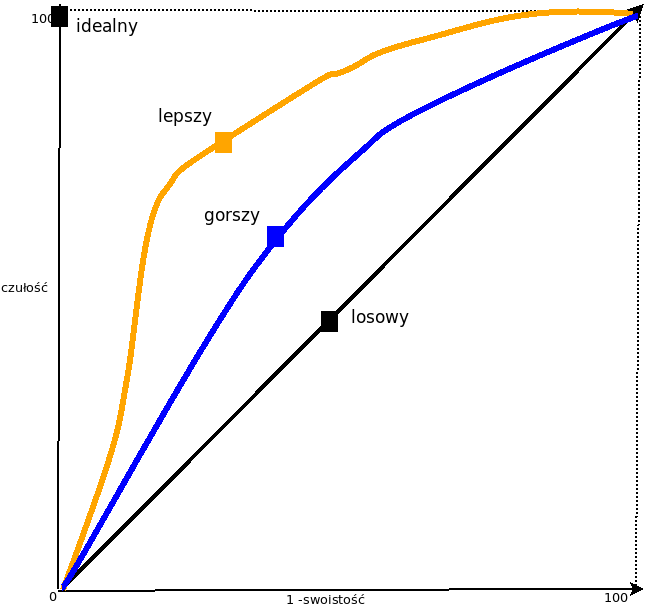
\includegraphics[width=0.75\linewidth]{./ROCcurve} \caption{Krzywa ROC}\label{fig:ROCcurve}
\end{figure}

\begin{example}
\textbf{Osteoporoza i witamina D}

Al Zarooni A.A.R i inni badali wpływ różnych czynników na ryzyka na
wystąpienie osteoporozy (Risk factors for vitamin D deficiency
in Abu Dhabi Emirati population; \url{https://doi.org/10.1371/journal.pone.0264064}),
takich jak deficyt witaminy D, wiek oraz płeć w grupie \text{392} osób.

Zacznijmy od modelu zerowego tj. takiego w którym ryzyko/prawdopodobieństwo/szansa
wystąpienia osteoporozy jest takie same bez względu na wielkości innych zmiennych.
Odpowiada to następującemu równaniu:

\[\ln(o) = b_0\]

W tabeli zestawiono wartości parametrów oszacowanego modelu, ilorazy szans, przedziału ufności
oraz prawdopodobieństwo.

\begin{tabular}{lrrrr}
\toprule
Parametr & Ocena & SE & z & p\\
\midrule
(Intercept) & -2,644537 & 0,2029618 & -13,02973 & 0\\
\bottomrule
\end{tabular}

Można obliczyć że (teoretyczne) prawdopodobieństwo wystąpienia osteoporozy
wyniosło \text{0,0663265}. Krzywa ROC dla modelu zerowego wygląda następująco:

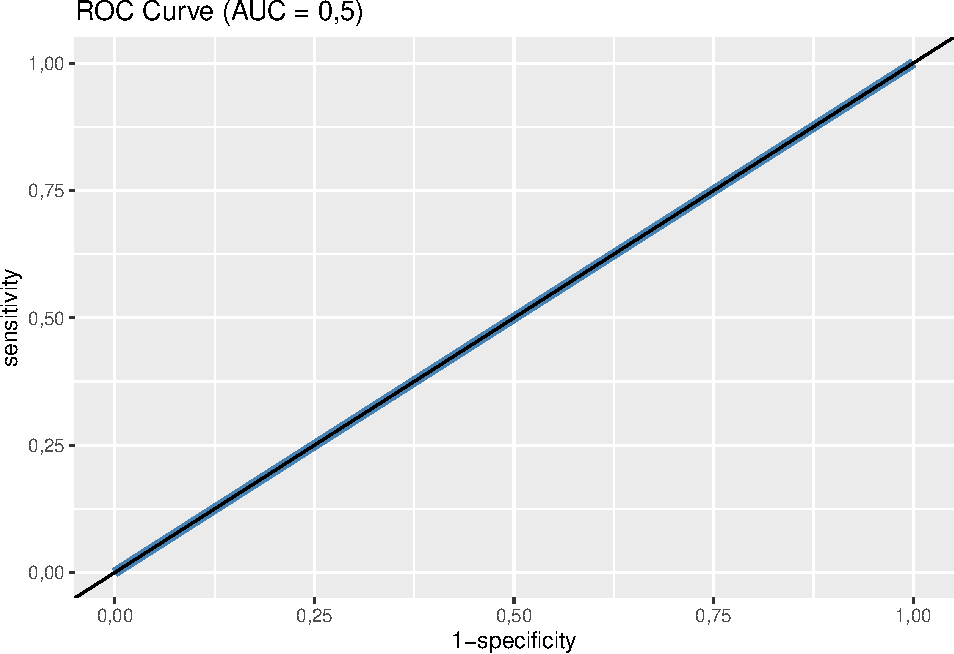
\includegraphics[width=0.75\linewidth]{_main_files/figure-latex/unnamed-chunk-70-1}

Model zerowy jak sama nazwa wskazuje może tylko służyć do porównania
z bardziej skomplikowanymi modelami.

Takim bardziej skomplikowanym modelem będzie przykładowo
zależność pomiędzy wystąpieniem osteoporozy a płcią, którą
można opisać następującym równaniem regresji:

\[\ln(o) = b_0 + b_1 \textrm{kobieta}\]

Zmienna \texttt{kobieta} przyjmuje wartość 1 jeżeli osoba była kobietą
oraz zero w przypadku jeżeli była mężczyzną.
Dla przypomnienia \(o\) jest szansą wystąpienia osteoporozy.

W tabeli zestawiono wartości parametrów oszacowanego modelu, ilorazy szans, przedziału ufności
oraz prawdopodobieństwo.

\begin{tabular}{lrrrrrl}
\toprule
Parametr & Ocena & SE & z & p & OR & CI\\
\midrule
(Intercept) & -3,367 & 0,455 & -7,403 & 0,000 & 0,03 & 0,01 0,08\\
genderF & 1,014 & 0,509 & 1,992 & 0,046 & 2,76 & 1,09 8,40\\
\bottomrule
\end{tabular}

Znając wartości współczynników równania można obliczyć wartości \(\ln(o)\).

Dewiancja modelu jest istotnie mniejsza od modelu zerowego (wartość \(p\) wynosi bowiem \text{0,0303521}).

Zależność pomiędzy wystąpieniem osteoporozy a płcią, wiekiem oraz poziomem witaminy D
można opisać następującym równaniem regresji:

\[\ln(o) = b_0 + b_1 \textrm{kobieta} + b_2 \textrm{wiek} + b_3 \textrm{poziomD}\]

W tabeli zestawiono wartości parametrów oszacowanego modelu, ilorazy szans, przedziału ufności
oraz prawdopodobieństwo.

\begin{tabular}{lrrrrrl}
\toprule
Parametr & Ocena & SE & z & p & OR & CI\\
\midrule
(Intercept) & -12,183 & 1,766 & -6,898 & 0,000 & 0,00 & 0,00  0,00\\
d & 0,005 & 0,009 & 0,536 & 0,592 & 1,00 & 0,99  1,02\\
age & 0,156 & 0,026 & 5,930 & 0,000 & 1,17 & 1,12  1,24\\
genderF & 2,463 & 0,662 & 3,722 & 0,000 & 11,74 & 3,54 48,76\\
\bottomrule
\end{tabular}

Macierz pomyłek (\emph{confussion matrix})

\begin{verbatim}
##         Osteoporoza
## Prognoza   0   1
##        0 362  22
##        1   4   4
\end{verbatim}

Stąd: czułość \text{0,1538462}; swoistość \text{0,989071}.

Istotność modelu:
dewiancja jest istotnie mniejsza od dewiancji modelu zerowego (p = \text{0}).

Krzywa ROC

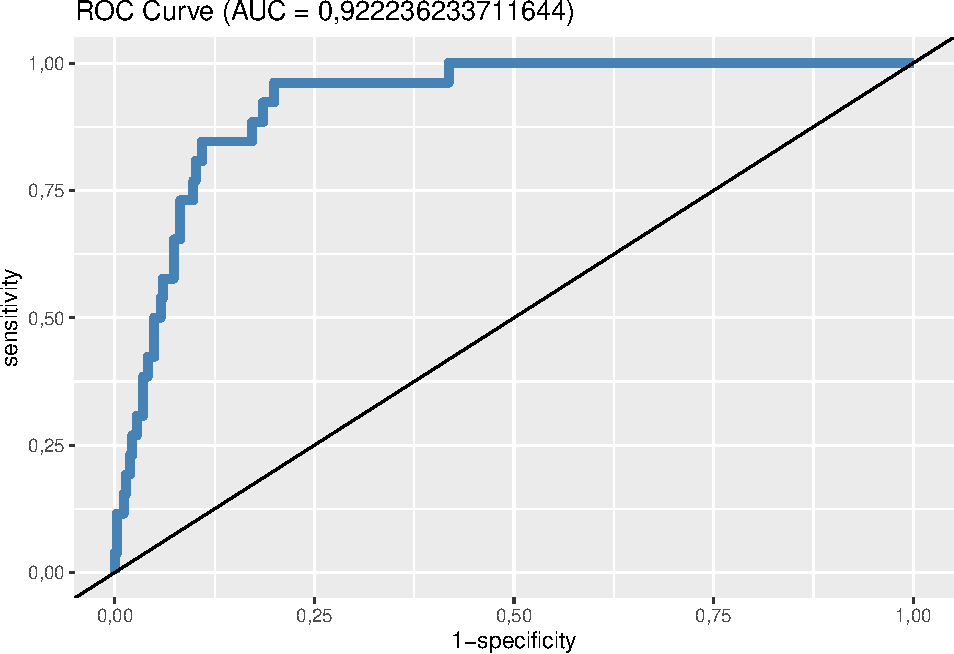
\includegraphics[width=0.75\linewidth]{_main_files/figure-latex/unnamed-chunk-76-1}
\end{example}

\hypertarget{przypadek-specjalny-co-najmniej-dwie-zmienne-porzux105dkowe}{%
\section{Przypadek specjalny: co najmniej dwie zmienne porządkowe}\label{przypadek-specjalny-co-najmniej-dwie-zmienne-porzux105dkowe}}

\hypertarget{pomiar-siux142y-zaleux17cnoux15bci-wspuxf3ux142czynnik-korelacji-rang}{%
\subsection{Pomiar siły zależności: współczynnik korelacji rang}\label{pomiar-siux142y-zaleux17cnoux15bci-wspuxf3ux142czynnik-korelacji-rang}}

Współczynnik korelacji rang Spearmana (\emph{Spearman's Rank-Order Correlation})
może być stosowany
w przypadku gdy cechy są mierzone w skali porządkowej (lub lepszej czyli liczbowej).

Obliczenie współczynnika Spearmana dla \(N\) obserwacji na zmiennych \(XY\)
polega na zamianie wartości
zmiennych \(X\) oraz \(Y\) na \textbf{rangi} (numery porządkowe od \(1\) do \(N\)).
Następnie stosowana jest formuła współczynnika korelacji
liniowej Pearsona (\(\tau_x\) oraz \(\tau_y\) oznaczają \textbf{rangi}):

\[\rho_{xy} = \frac{\textrm{cov}(\tau_x, \tau_y)}{s_{\tau_x}  s_{\tau_y}}\]

Współczynnik \(\rho_{xy}\) to -- podobnie jak \textbf{oryginalny} współczynnik
korelacji liniowej Pearsona -- miara niemianowana, o wartościach
ze zbioru {[}-1;1{]}.

\begin{example}
\textbf{Spożycie mięsa}

Współczynnik Pearsona i Spearmana dla zależności między spożyciem mięsa w 1980
a spożyciem mięsa w 2013 roku (zmienna objaśniana):

\begin{itemize}
\item
  współczynnik Pearsona: \text{0,68};
\item
  współczynnik Spearmana: \text{0,68}.
\end{itemize}

Nie ma sensu liczenia współczynnika korelacji rang w przypadku kiedy obie
cechy są liczbami, bo wtedy należy użyć normalnego współczynnika Pearsona.
Ale nie jest to też błędem więc w powyższym przykładzie go liczymy.

Współczynnik korelacji liniowej Spearmana
wynosi \text{0,68} (umiarkowana korelacja).

Czy ta wartość jest istotnie różna od zera? Jest na to stosowny
test statystyczny, który sprowadza się do określenia jakie jest
prawdopodobieństwo otrzymania \(r_s\) = \text{0,68} przy założeniu że
prawdziwa wartość \(r_s\) wynosi zero. Otóż w naszym przykładzie
to prawdopodobieństwo wynosi 2.302116e-26
(czyli jest ekstremalnie małe -- współczynnik jest istotnie różny od zera).
\end{example}

\hypertarget{podsumowanie}{%
\section{Podsumowanie}\label{podsumowanie}}

Przedstawiono 7 następujących metod ustalania zależności między zmiennymi:

\begin{enumerate}
\def\labelenumi{\arabic{enumi}.}
\item
  Wykres rozrzutu.
\item
  Tablica wielodzielna i test chi-kwadrat.
\item
  Współczynnik korelacji liniowej Pearsona.
\item
  Współczynnik korelacji Spearmana.
\item
  Regresja liniowa.
\item
  Regresja logistyczna.
\item
  testy \(t\) Welcha, U Manna-Whitneya, ANOVA albo test Kruskala-Wallisa.
\end{enumerate}

\hypertarget{surveyexamples}{%
\chapter{Przykłady badań ankietowych}\label{surveyexamples}}

Uwaga: ankieta nie jest kolejną metodą statystyczną tylko techniką zbierania danych.
Wszystkie metody już zostały przedstawione i żadnej nowej nie będzie.

\hypertarget{jak-zaczux105ux107-badanie}{%
\section{Jak zacząć badanie?}\label{jak-zaczux105ux107-badanie}}

Każde badanie, w tym ankietowe.

Należy zastanowić się nad trzema sprawami:

\begin{enumerate}
\def\labelenumi{\arabic{enumi}.}
\item
  Co chcemy ustalić?
\item
  Jakie dane są nam potrzebne, żeby ustalić to co chcemy ustalić?
\item
  Jak te dane zebrać (czyli co i w jaki sposób zmierzyć)?
\end{enumerate}

\textbf{Co chcemy ustalić?}

Najlepiej jakąś zależność. Na przykład: stress a wypalenie zawodowe;
satysfakcja zawodowa a retencja; determinanty satysfakcji zawodowej.

Może być od biedy opis czegoś lub porównanie czegoś z czymś. Przykłady:
nadwaga wśród studentów wydziału zdrowia PSW; analiza porównawcza
wypalenia zawodowego pielęgniarek
pracujących w różnych systemach opieki.

\textbf{Co i jak mierzyć?}

Jeżeli mamy zamiar badać nadwagę, to powinniśmy zmierzyć masę ciała.
Jeżeli celem jest ustalenie zależności pomiędzy stresem a wypaleniem
zawodowym to niewątpliwie powinniśmy zmierzyć stress i wypalenia. Jak
dotąd banalnie prosto. Problem zaczyna się w momencie odpowiedzi na
pytanie \textbf{jak}?

\hypertarget{mierzenie-twardych-faktuxf3w-vs-mierzenia-przekonaux144}{%
\subsection{Mierzenie twardych faktów vs mierzenia przekonań}\label{mierzenie-twardych-faktuxf3w-vs-mierzenia-przekonaux144}}

Możemy pytać w ankiecie o dwie rzeczy:

\begin{itemize}
\item
  \textbf{fakty} (wiek, staż, zawód, tętno, przebyte choroby);
\item
  \textbf{przekonania}, \textbf{wartości}, \textbf{postawy};
  \textbf{uczucia} (strach / radość) albo \textbf{zamiary}
  (w języku attitudes/emotions/intentions).
\end{itemize}

Mierzenie \textbf{faktów} nie wymaga dodatkowych objaśnień. Problem jest
z mierzeniem \textbf{przekonań}.

\textbf{Przekonanie} to idea, którą jednostka uważa
za prawdziwą. \textbf{Wartości} to trwałe przekonania o tym,
co jest ważne dla jednostki. Stają się standardami, według których jednostki dokonują wyborów.
\textbf{Postawy} to mentalne dyspozycje/nastawienie
przed podjęciem decyzji, które skutkują
określonym zachowaniem (zrobię to a nie tamto). Postawy
kształtowane są wartościami i przekonaniami.

\hypertarget{pomiar-przekonaux144-wartoux15bci-i-postaw}{%
\subsection{Pomiar przekonań, wartości i postaw}\label{pomiar-przekonaux144-wartoux15bci-i-postaw}}

Postawy/uczucia/zamiary są to pojęcia
abstrakcyjne. Często (albo zawsze) definiowane w obszarze psychologii,
nauk o zarządzaniu itp.

Pomiar \emph{przekonań} jest dokonywany w specyficzny sposób.
\textbf{Definicja konceptualna} definiuje pojęcie
(zaufanie do kogoś/czegoś to \textbf{przekonanie}, że
\emph{działania tego kogoś/czegoś okażą się zgodne z naszymi
oczekiwaniami}; satysfakcja to
\textbf{uczucie} \emph{przyjemności, zadowolenia z czegoś};
samoskuteczność to
\textbf{przekonanie}, iż \emph{jest się w stanie zrealizować określone działanie lub osiągnąć wyznaczone cele}).
\textbf{Definicja operacyjna} określa jak zmierzyć pojęcie
(jak zmierzyć satysfakcję)
Przejście od definicji konceptualnej do definicji operacyjnej
bywa czasami mocno, hmm\ldots{} arbitralne.

\hypertarget{skala-likerta}{%
\subsection{Skala Likerta}\label{skala-likerta}}

Przykładowo chcemy się dowiedzieć czy i jak bardzo respondenci boją się COVID19.

W najprostszej wersji się po prostu pytamy:
\textbf{Czy pan/pani boi się COVID19?} i dajemy
respondentowi trzy możliwe warianty odpowiedzi: Tak/Nie/Nie wiem.
Taki pomiar jest mocno zgrubny: ktoś
się może bać panicznie a ktoś inny dużo mniej.

Subtelniejszy pomiar to wybór spośród pięciu wariantów:
bardzo się boję -- boję się -- trudno powiedzieć -- nie boję się -- zupełnie się nie boję.

Taką skalę pomiarową określamy jak wiemy jako \textbf{porządkową}. Pomiary nie są liczbami,
ale są uporządkowane.
Rangi wartości są już liczbami (np. 1--5 w przykładowej skali pięciowariantowej),
można je np. uśredniać.
Tego typu skala pomiarowa, typowa dla ankiet, nosi nazwę skali \textbf{Likerta}.
Można sobie wymyślać skalę Likerta 7-punktową i więcej.

Naszym zdaniem powyżej 7 wariantów normalny respondent będzie miał problem
czy się bardziej-bardziej czy jednak bardziej-bardziej-bardziej boi.

\hypertarget{skala-pomiarowa-czyli-inwentarz-albo-kwestionariusz}{%
\subsection{Skala pomiarowa czyli inwentarz albo kwestionariusz}\label{skala-pomiarowa-czyli-inwentarz-albo-kwestionariusz}}

Ponieważ skala Likerta, mimo że lepsza od pytań tak/nie, jest ciągle zgrubna, to
uważa się powszechnie, że lepszy wynik da pomiar
wielokrotny.
W naukach podstawowych mierzymy (np. linijką) parę razy, a wynik uśredniamy co daje pomiar bardziej precyzyjny. Tutaj pytamy się parę razy o to samo co
ma dać podobny efekt (mniejszy średni błąd pomiaru).
Taka seria pytań nosi też nazwę skali albo \textbf{inwentarza}.
Nie pytamy się zatem \textbf{Czy pan/pani boi się COVID19?} tylko zadajemy serię
pytań o strach względem COVID19:

\begin{example}
\textbf{Strach przed COVID19}

The Fear of COVID-19 Scale: Development and Initial Validation.
International Journal of
Mental Health and Addiction, 1--9.
(\url{https://www.ncbi.nlm.nih.gov/pmc/articles/PMC7100496/}).

Lęk przed koronawirusem COVID-19
i lęk przed śmiercią -- polskie adaptacje narzędzi
(\url{https://www.termedia.pl/Fear-of-COVID-19-and-death-anxiety-Polish-adaptations-of-scales,116,44937,1,1.html}).

\begin{enumerate}
\def\labelenumi{\arabic{enumi}.}
\item
  I am most afraid of Corona.
\item
  It makes me uncomfortable to think about Corona.
\item
  My hands become clammy when I think about Corona.
\item
  I am afraid of losing my life because of Corona.
\item
  When I watch news and stories about Corona on social media, I become nervous or anxious.
\item
  I cannot sleep because I'm worrying about getting Corona.
\item
  My heart races or palpitates when I think about getting Corona.
\end{enumerate}

albo:

\begin{enumerate}
\def\labelenumi{\arabic{enumi}.}
\item
  Boję się koronawirusa.
\item
  Czuję dyskomfort, gdy myślę o koronawirusie.
\item
  Pocą mi się dłonie, gdy myślę o koronawirusie.
\item
  Boję się, że mogę stracić życie z powodu koronawirusa.
\item
  Gdy oglądam wiadomości i czytam o koronawirusie w mediach
  społecznościowych, robię się nerwowy i niespokojny.
\item
  Nie mogę spać, ponieważ martwię się, że ja lub moi bliscy zarażą się.
\item
  Dostaję palpitacji serca, gdy myślę o tym, że mógłbym się zarazić.
\end{enumerate}

Odpowiadający ma do wyboru pięć wariantów odpowiedzi:
\textbf{zdecydowanie nie}/\textbf{nie}/\textbf{nie mam zdania}/\textbf{tak}/\textbf{zdecydowanie tak}.
\end{example}

\hypertarget{model-pomiaru}{%
\subsection{Model pomiaru}\label{model-pomiaru}}

\textbf{Ukryty czynnik} (strach) kształtuje wartości \textbf{indykatorów} (odpowiedzi na pytania)
Taki sposób pomiaru \textbf{ukrytego czynnika} (\emph{latent} w języku angielskim) określa się
mianem refleksyjnego (co jest kalką od \emph{reflexive}). Na rysunku \ref{fig:modelP}
kierunek strzałki obrazuje zależność (czynnik→indykator).

\begin{figure}
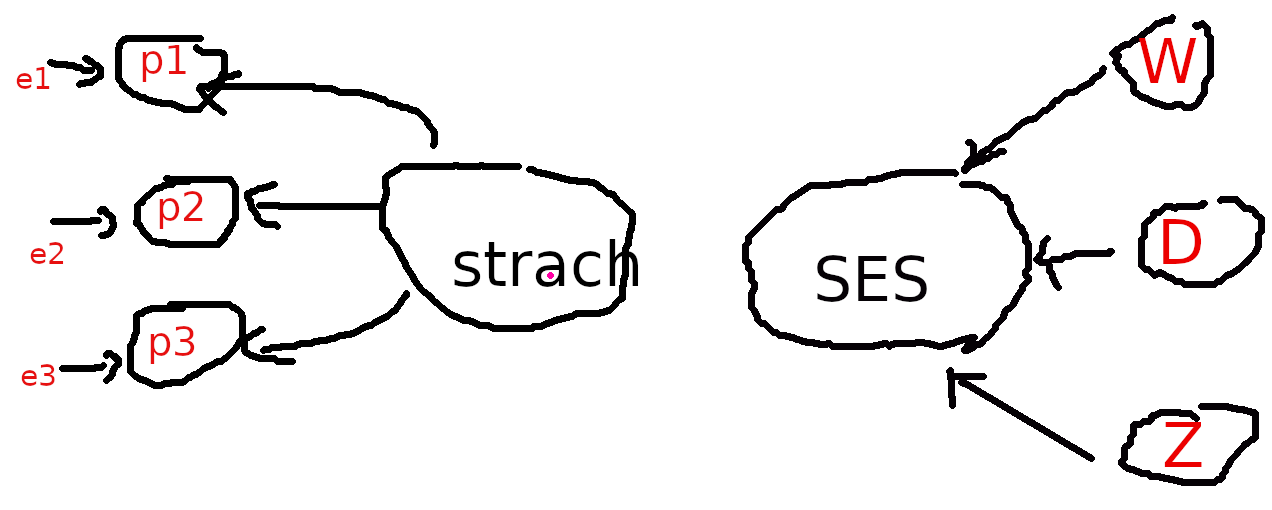
\includegraphics[width=0.9\linewidth]{./pomiar_ses-cropped} \caption{Modele pomiaru czynnika ukrytego}\label{fig:modelP}
\end{figure}

Alternatywny sposób definiowania ukrytego (w pewnym sensie, raczej złożonego)
czynnika nosi nazwę \textbf{formatywnego} (albo indeksu): czynnik jest sumą indykatorów.
Przykładem może być SES:
status socjo-ekonomiczny będący agregatem wykształcenia (W), dochodu (D)
oraz zawodu (Z).

W założeniu indykatory są jednakowo dobrymi miarami
czynnika refleksyjnego i jako takie powinny być mocno
skorelowane (mierzą to samo).
Natomiast składniki czynnika formatywnego nie powinny
być skorelowane, raczej każdy powinien mierzyć \textbf{inny
aspekt} czynnika. Ktoś może być profesorem
za przeproszeniem filozofii, nie mieć pracy i kiepskie
dochody.
Tylko jeden z trzech aspektów podwyższa mu SES;
albo świetnie zarabiająca prostytutka bez matury.

Jeżeli w czynniku refleksyjnym pominiemy jeden z trzech indykatorów, to nic się
nie stanie oprócz tego, że pomiar będzie mniej precyzyjny. Jeżeli
w czynniku formatywnym pominiemy indykator, to popełniamy gruby błąd, bo pomijamy
istotny składnik całości.

Dobrą wiadomością jest, że najprostszy sposób pomiaru traktuje czynniki
refleksyjne i formatywne jednakowo: wartością czynnika jest suma albo ewentualnie średnia
wartość indykatorów. Jeżeli indykatory są mierzone za pomocą skali Likerta
suma (albo średnia) wartości rang po prostu. W skali strachu przed COVID ten kto się najbardziej
boi powinien odpowiedzieć 7 razy \textbf{zdecydowanie tak}, co odpowiada
sumie 35 rang (jeżeli rangujemy od 1 do 5).
Ten który się wcale nie boi zaś będzie miał 7.

Małym utrudnieniem mogą być \textbf{pytania odwrócone}. Jeżeli pytamy
o strach przed COVID i w każdym pytaniu jak bardzo ktoś się boi, albo jak
bardzo mu serce bije, ale w jednym z pytań zapytamy \textbf{nie boję się COVID},
to ranga 5 odpowiada uczuciu \textbf{braku strachu}. Rangi w pytaniach odwróconych
należy przeliczyć (odwrócić): 1 zamienić na 5, 2 na 4 itd\ldots{}
Jeżeli używamy cudzych skal to w opisie powinno być wskazane, które
pytania są odwrócone.

\textbf{Zalecany schemat postępowania jeżeli w ankiecie mają być mierzone
przekonania} (strach, samoskuteczność, wypalenie zawodowe, stress czy satysfakcja):

\begin{itemize}
\item
  Dokształcamy się nieco z psychologii mimo wszystko;
\item
  Robimy przegląd literatury i znajdujemy skalę, którą ktoś już wymyślił żeby
  mierzyć to co my chcemy zmierzyć, bo \textbf{raczej nie należy wymyślać własnych skal};
\item
  Robimy ankietę (w Internecie) i zbieramy dane;
\item
  Wykonujemy analizę statystyczną.
\end{itemize}

Banalnie proste co udowodnimy na przykładach.

\hypertarget{wiedza-na-temat-szkodliwoux15bci-palenia-i-jej-uwarunkowania-wux15bruxf3d-studentuxf3w-psw}{%
\section{Wiedza na temat szkodliwości palenia i jej uwarunkowania wśród studentów PSW}\label{wiedza-na-temat-szkodliwoux15bci-palenia-i-jej-uwarunkowania-wux15bruxf3d-studentuxf3w-psw}}

\hypertarget{cel}{%
\subsection{Cel}\label{cel}}

Celem jest ocena wielkości zjawiska palenia tytoniu oraz
poziom wiedzy na temat szkodliwości palenia tytoniu
wśród
studentów PSW oraz zweryfikowanie wpływu wybranych czynników warunkujących ten nałóg.

\textbf{Postawiono następujące hipotezy badawcze}:

\begin{enumerate}
\def\labelenumi{\arabic{enumi}.}
\item
  Jaka jest wielkość zjawiska palenie tytoniu wśród studentów PSW?
\item
  Jaka jest wiedza na temat szkodliwości palenia tytoniu wśród studentów PSW?
\item
  Czy palenie jest skorelowane z płcią, stażem pracy i miejscem pracy?
\item
  Czy wiedza na temat szkodliwości palenie jest skorelowana z płcią, stażem pracy i miejscem pracy?
\item
  Czy palenie jest skorelowane z wiedzą na temat szkodliwości palenia?
\end{enumerate}

\hypertarget{metoda}{%
\subsection{Metoda}\label{metoda}}

Badanie ankietowe wśród studentów Ratownictwa Medycznego (RM) oraz Pielęgniarstwa (PO)
przeprowadzono w styczniu 2023.
Ankieta zawierała pytania dotyczące palenia tytoniu (pali/nie pali/palił, jak długo pali itd),
test wiedzy na temat szkodliwości palenia oraz pytania
o rodzaj miejsca pracy, staż pracy i płeć itd.

Pięć następujących pytań oceniało wiedzę ankietowanego na temat szkodliwości palenia:

\begin{itemize}
\tightlist
\item
  Czy bardziej szkodliwe dla zdrowia jest czynne czy bierne palenie? (JW);
\item
  Jakie według Ciebie choroby układu oddechowego mogą być spowodowane
  bezpośrednio przez palenie papierosów? (WW);
\item
  Czy palenie papierosów powoduje choroby układu pokarmowego? (JW);
\item
  Jakie według Ciebie choroby kardiologiczne mogą być spowodowane
  bezpośrednio przez palenie papierosów? (WW);
\item
  Jaki według Ciebie ma wpływ palenie papierosów na narządy zmysłów? (WW).
\end{itemize}

W przypadku pytań jednokrotnego wyboru (JW), za wskazanie poprawnej
odpowiedzi respondent otrzymywał 1 punkt.
W przypadku pytań wielokrotnego wyboru (WW) za wskazanie prawidłowej odpowiedzi
respondent otrzymywał 1 punkt, ale
za wskazanie nieprawidłowej
otrzymywał (minus) -1 punkt (aby nie opłacała się strategia zaznaczenia wszystkich odpowiedzi).
Maksymalna możliwa do uzyskania liczba punktów wynosiła 19.

\hypertarget{zastosowane-metody-statystyczne}{%
\subsection{Zastosowane metody statystyczne}\label{zastosowane-metody-statystyczne}}

\begin{itemize}
\item
  Hipotezę 1 weryfikowano na podstawie wielkości odsetka respondentów palących.
\item
  Hipotezę 2 weryfikowano na podstawie wielkości odsetka respondentów wykazujących się
  dobrą i bardzo dobrą wiedzą na temat palenia.
\item
  Hipotezy 3--5 zweryfikowano z wykorzystaniem tablic wielodzielnych/testu chi-kwadrat
  oraz porównania średniego poziomu depresji w grupach za pomocą testów Manna-Whitneya oraz
  Kruskala-Wallisa.
\end{itemize}

\hypertarget{metryczka-analiza-respondentuxf3w}{%
\subsection{Metryczka (analiza respondentów)}\label{metryczka-analiza-respondentuxf3w}}

Rozkład ankietowanych wg wyniku testu
na znajomość szkodliwości palenia przedstawiono na rysunku \ref{fig:rysunek51}.

\begin{figure}
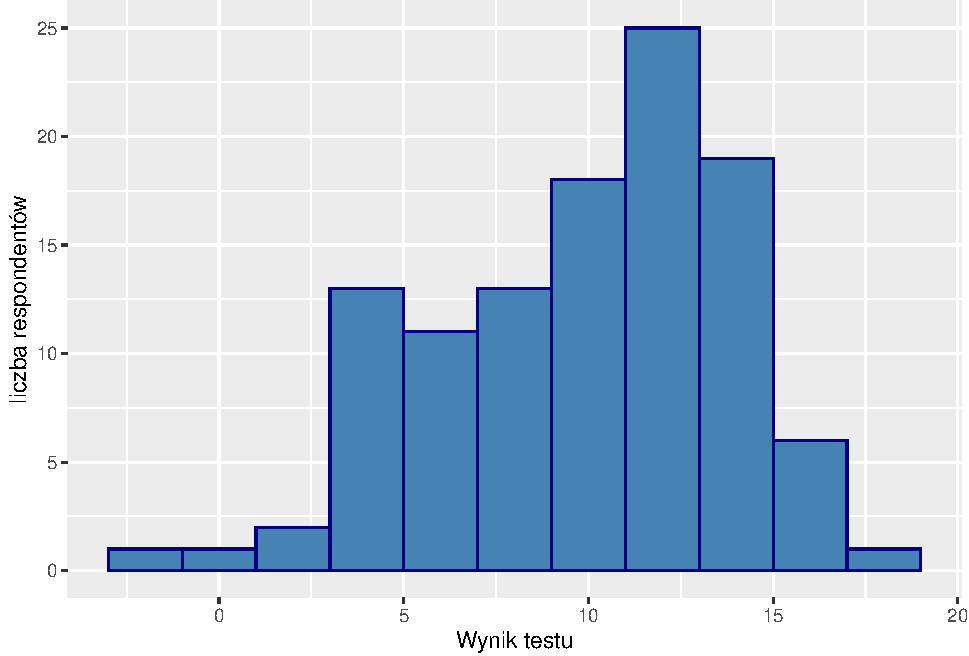
\includegraphics[width=0.85\linewidth]{_main_files/figure-latex/rysunek51-1} \caption{Studenci wg wyniku testu na znajomość szkodliwości palenia}\label{fig:rysunek51}
\end{figure}

W badaniu wzięło udział \text{110} studentów.
Otrzymano \text{110} poprawnie
wypełnionych ankiet. Średnia wartość testu oceniającego wiedzę
wyniosła \text{10,364} (odchylenie
standardowe \text{3,997}).

Rozkład ankietowanych ze względu na status względem
palenia przedstawiono na rysunku \ref{fig:rysunek52}.

\begin{figure}
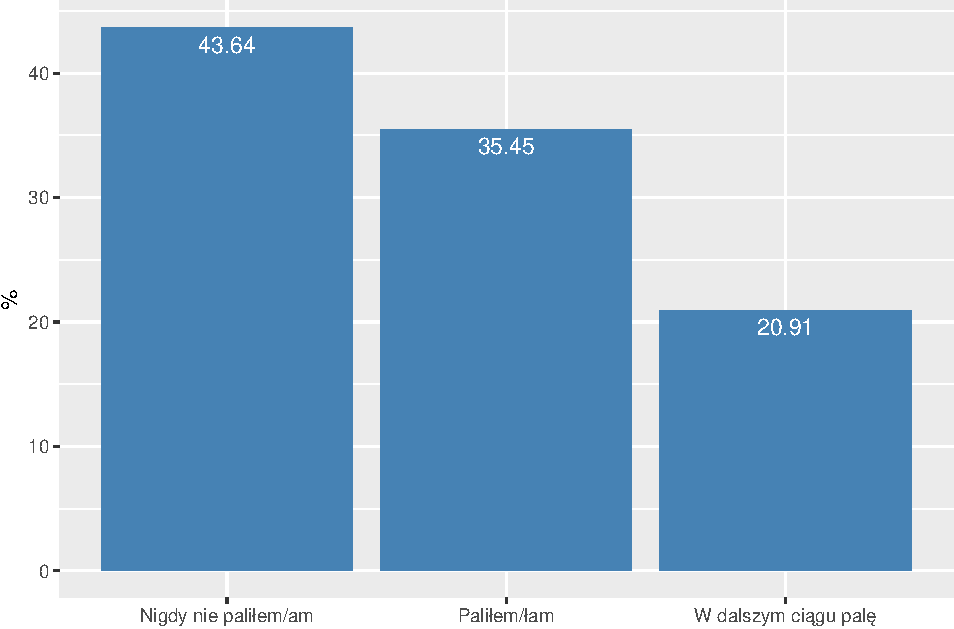
\includegraphics[width=0.85\linewidth]{_main_files/figure-latex/rysunek52-1} \caption{Studenci wg statusu palenia (\%)}\label{fig:rysunek52}
\end{figure}

Rozkład ankietowanych ze względu na staż pracy przedstawiono na rysunku \ref{fig:rysunek54}.

\begin{figure}
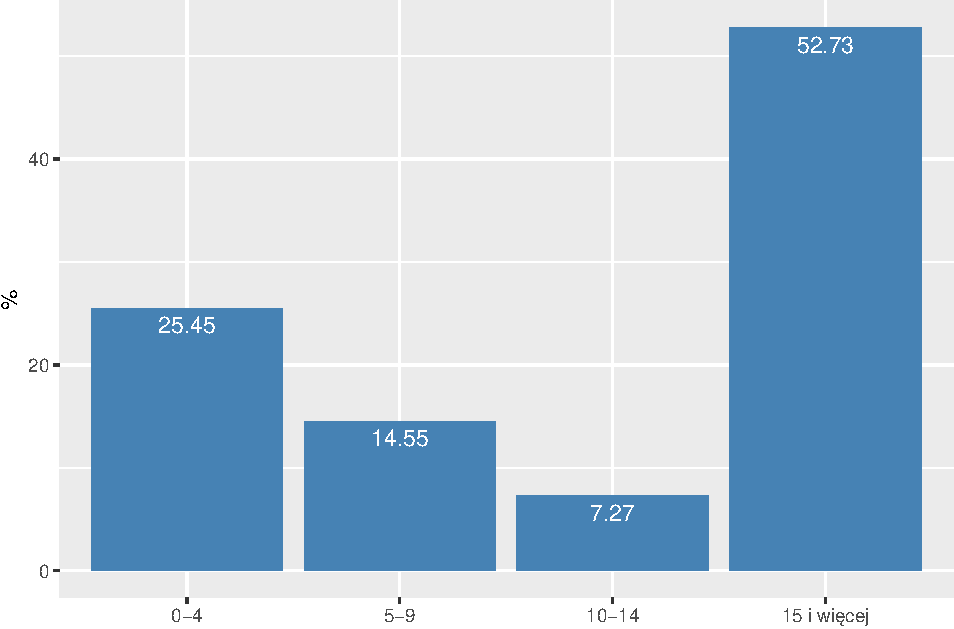
\includegraphics[width=0.85\linewidth]{_main_files/figure-latex/rysunek54-1} \caption{Studenci wg stażu pracy (\%)}\label{fig:rysunek54}
\end{figure}

Zmienna płeć i miejsce pracy są dwuwartościowe, więc (oszczędzając lasy)
proponujemy zamiast wykresu
poprzestanie na podaniu odsetka kobiet/mężczyzn oraz pracowników szpitali/przychodni.

Zatem wśród respondentów było \text{70}\% kobiet i \text{30}\% mężczyzn.
Pracę w szpitalu zadeklarowało \text{90}\% respondentów a w przychodni
\text{10}\% respondentów.

\hypertarget{weryfikacja-hipotezy-1}{%
\subsection{Weryfikacja hipotezy 1}\label{weryfikacja-hipotezy-1}}

Palą lub paliło 62 respondentów
(56.36 \%).
Żeby stwierdzić czy to jest dużo czy mało to na przykład można by porównać
z jakąś średnią ogólnopolską.

\hypertarget{weryfikacja-hipotezy-2}{%
\subsection{Weryfikacja hipotezy 2}\label{weryfikacja-hipotezy-2}}

Średnia wartość uzyskana w teście wyniosła \text{10,36}
(mediana \text{11}); 3/4 respondentów nie uzyskało więcej niż
\text{13} (czyli \text{68,4} \%).

\hypertarget{weryfikacja-hipotez-35}{%
\subsection{Weryfikacja hipotez 3--5}\label{weryfikacja-hipotez-35}}

Czy palenie jest skorelowane z płcią?

\begin{tabular}{lrr}
\toprule
  & K & M\\
\midrule
Nigdy nie paliłem/am & 31 & 17\\
Paliłem/łam & 27 & 12\\
W dalszym ciągu palę & 19 & 4\\
\bottomrule
\end{tabular}

\begin{verbatim}
## 
##  Pearson's Chi-squared test
## 
## data:  t.sex.f
## X-squared = 2,4228, df = 2, p-value = 0,2978
\end{verbatim}

Nie jest o czym świadczy wysoka wartość p (\text{0,2978}).

Czy palenie jest skorelowane ze stażem pracy?

\begin{tabular}{lrrrr}
\toprule
  & 0-4 & 5-9 & 10-14 & 15 i więcej\\
\midrule
Nigdy nie paliłem/am & 14 & 6 & 4 & 24\\
Paliłem/łam & 8 & 6 & 2 & 23\\
W dalszym ciągu palę & 6 & 4 & 2 & 11\\
\bottomrule
\end{tabular}

\begin{verbatim}
## 
##  Pearson's Chi-squared test
## 
## data:  t.staz.f
## X-squared = 1,7687, df = 6, p-value = 0,9397
\end{verbatim}

Nie jest o czym świadczy wysoka wartość p (\text{0,9397}).

Czy palenie jest skorelowane z miejscem pracy?

\begin{tabular}{lrr}
\toprule
  & Przychodnia & Szpital\\
\midrule
Nigdy nie paliłem/am & 5 & 43\\
Paliłem/łam & 3 & 36\\
W dalszym ciągu palę & 3 & 20\\
\bottomrule
\end{tabular}

\begin{verbatim}
## 
##  Pearson's Chi-squared test
## 
## data:  t.praca.f
## X-squared = 0,47674, df = 2, p-value = 0,7879
\end{verbatim}

Nie jest o czym świadczy wysoka wartość p (\text{0,7879}).

Czy wiedza na temat palenia jest skorelowana z płcią?

\begin{tabular}{lrrr}
\toprule
płeć & średnia & mediana & n\\
\midrule
K & 10,831169 & 12 & 77\\
M & 9,272727 & 10 & 33\\
\bottomrule
\end{tabular}

Sprawdzamy czy rozkłady są normalne:

\begin{tabular}{lrr}
\toprule
płeć & S-W & p\\
\midrule
K & 0,9325443 & 0,0005147\\
M & 0,9295526 & 0,0339828\\
\bottomrule
\end{tabular}

Nie są. Należy zastosować test U Manna-Whitneya:

\begin{verbatim}
## $p.value
## [1] 0,04883299
\end{verbatim}

Wartość p wynosi \text{0,048833}, zatem
hipotezę o braku zależności na poziomie 0,05 należy odrzucić.
Istnieje zależność pomiędzy wiedzą na temat palenia a płcią. Kobiety
wykazują się wyższą wiedzą na temat szkodliwości palenia od mężczyzn.

Czy wiedza na temat palenia jest skorelowana z miejscem pracy?

\begin{tabular}{lrrr}
\toprule
m.pracy & średnia & mediana & n\\
\midrule
Przychodnia & 10,36364 & 10 & 11\\
Szpital & 10,36364 & 11 & 99\\
\bottomrule
\end{tabular}

Sprawdzamy czy rozkłady są normalne:

\begin{tabular}{lrr}
\toprule
m.pracy & S-W & p\\
\midrule
Przychodnia & 0,9272191 & 0,3834099\\
Szpital & 0,9590504 & 0,0036563\\
\bottomrule
\end{tabular}

Nie są. Należy zastosować test U Manna-Whitneya:

\begin{verbatim}
## [1] 0,8026325
\end{verbatim}

Wartość p wynosi \text{0,8026325} -- nie ma podstaw
od odrzucenia hipotezy o identyczności rozkładów na poziomie p = 0,05. Nie ma różnicy
w poziomie wiedzy wśród pracowników przychodni i szpitali.

Czy wiedza na temat palenia jest skorelowana ze stażem?

\begin{tabular}{lrrr}
\toprule
staż & średnia & mediana & n\\
\midrule
0-4 & 9,928571 & 10,0 & 28\\
5-9 & 9,812500 & 11,0 & 16\\
10-14 & 9,875000 & 11,0 & 8\\
15 i więcej & 10,793103 & 11,5 & 58\\
\bottomrule
\end{tabular}

Sprawdzamy czy rozkłady są normalne:

\begin{tabular}{lrr}
\toprule
staż & S-W & p\\
\midrule
0-4 & 0,9644460 & 0,4418353\\
5-9 & 0,8847339 & 0,0460152\\
10-14 & 0,8985547 & 0,2804097\\
15 i więcej & 0,9409402 & 0,0071265\\
\bottomrule
\end{tabular}

Nie są. Należy zastosować test Kruskala-Wallisa:

\begin{verbatim}
## [1] 0,6771844
\end{verbatim}

Wartość p wynosi \text{0,6771844} -- nie ma podstaw
od odrzucenia hipotezy o identyczności rozkładów na poziomie p = 0,05. Nie ma
różnicy w poziomie wiedzy wśród pracowników o różnym stażu pracy.

Czy wiedza o szkodliwości palenia jest skorelowana
ze statusem względem palenia? Chcemy zastosować tablicę wielodzielczą/test chi kwadrat. Musimy zatem zamienić skalę liczbową zmiennej mierzącej wiedzę nt szkodliwości palenia na nominalną, np tak:
0--5 mała; 6--10 średnia; 11--15 duża, 16--19 ogromna:

\begin{tabular}{lrrr}
\toprule
  & Nigdy nie paliłem/am & Paliłem/łam & W dalszym ciągu palę\\
\midrule
duża & 22 & 16 & 14\\
mała & 7 & 6 & 4\\
ogromna & 2 & 3 & 2\\
średnia & 17 & 14 & 3\\
\bottomrule
\end{tabular}

\begin{verbatim}
## 
##  Pearson's Chi-squared test
## 
## data:  wiedza.status.t
## X-squared = 4,9954, df = 6, p-value = 0,5444
\end{verbatim}

Wiedza i status względem palenia nie są skorelowane
o czym świadczy wysoka wartość p (\text{0,5444}).

Można to samo zweryfikować stosując test Kruskala-Wallisa:

\begin{tabular}{lrrr}
\toprule
status & średnia & mediana & n\\
\midrule
Nigdy nie paliłem/am & 10,31250 & 10,5 & 48\\
Paliłem/łam & 10,07692 & 10,0 & 39\\
W dalszym ciągu palę & 10,95652 & 12,0 & 23\\
\bottomrule
\end{tabular}

\begin{verbatim}
## [1] 0,7787663
\end{verbatim}

Wynik jest identyczny (wysoka wartość p \text{0,7788}).

\hypertarget{wnioski}{%
\subsection{Wnioski}\label{wnioski}}

\begin{itemize}
\item
  Ponad połowa studentów pali lub paliła.
\item
  Istnieje zależność pomiędzy wiedzą o szkodliwości palenia a płcią.
\item
  Nie ma związku pomiędzy statusem względem palenia a płcią, miejscem pracy i stażem.
\item
  Nie ma związku pomiędzy wiedzą o szkodliwości palenia a miejscem pracy i stażem.
\end{itemize}

\hypertarget{depresja-i-jej-uwarunkowania-wux15bruxf3d-studentuxf3w-psw}{%
\section{Depresja i jej uwarunkowania wśród studentów PSW}\label{depresja-i-jej-uwarunkowania-wux15bruxf3d-studentuxf3w-psw}}

\hypertarget{cel-1}{%
\subsection{Cel}\label{cel-1}}

Celem jest ustalenie czy depresja jest istotnym problemem wśród
studentów PSW oraz zweryfikowanie wybranych czynników warunkujących depresję.

\hypertarget{metoda-1}{%
\subsection{Metoda}\label{metoda-1}}

Badanie ankietowe wśród studentów Ratownictwa Medycznego (RM) oraz Pielęgniarstwa (PO)
przeprowadzono w styczniu 2023.
Ankieta zawierała test samooceny depresji Becka oraz pytania
o rodzaj miejsca pracy, staż pracy i płeć.

Test samooceny depresji Becka składa się z 21 pytań. W każdym pytaniu
możliwe są 4 warianty odpowiedzi, odpowiadające zwiększonej intensywności objawów depresji,
którym w związku z tym przypisuje się wartości od zera do 3 punktów. Maksymalna liczba punktów
w teście wynosi 63 a minimalna 0.

Interpretacja wyników testu Becka: 0--19 brak/łagodna depresja;
20--25 umiarkowana; 26--63 ciężka depresja.

Postawiono następujące hipotezy badawcze:

\begin{enumerate}
\def\labelenumi{\arabic{enumi}.}
\item
  Depresja stanowi duży problem wśród studentów PSW.
\item
  Problem depresji zależy od miejsca pracy.
\item
  Problem depresji zależy od stażu pracy.
\item
  Problem depresji zależy od płci.
\end{enumerate}

\hypertarget{zastosowane-metody-statystyczne-1}{%
\subsection{Zastosowane metody statystyczne}\label{zastosowane-metody-statystyczne-1}}

\begin{itemize}
\item
  Hipotezę 1 oceniono na podstawie odsetka respondentów wykazujących ciężką postać depresji.
\item
  Hipotezy 2--4 zweryfikowano z wykorzystaniem tablic wielodzielczych/testu chi-kwadrat
  oraz porównania poziomu depresji w grupach za pomocą testów Manna-Whitneya oraz
  Kruskala-Wallisa.
\end{itemize}

\hypertarget{metryczka}{%
\subsection{Metryczka}\label{metryczka}}

W badaniu wzięło udział \text{103} studentów. Otrzymano \text{103} poprawnie
wypełnionych ankiet. Średnia wartość testu Becka wyniosła \text{8,379} (odchylenie
standardowe \text{8,577}).

Rozkład ankietowanych wg wyniku testu Becka przedstawiono na rysunku \ref{fig:rysunek56}.

\begin{figure}
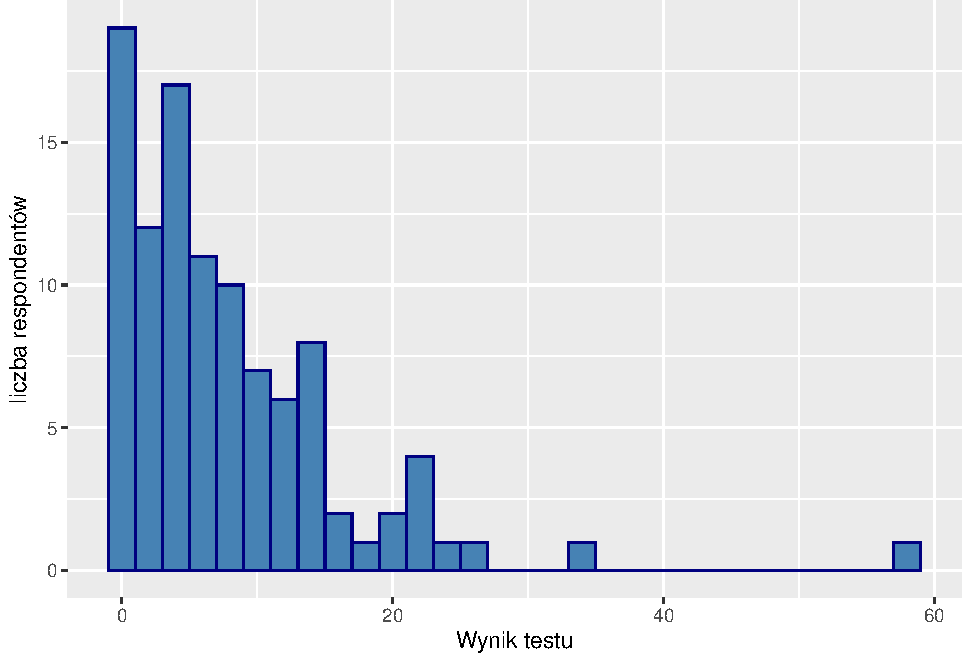
\includegraphics[width=0.85\linewidth]{_main_files/figure-latex/rysunek56-1} \caption{Studenci wg wyniku testu Becka}\label{fig:rysunek56}
\end{figure}

Rozkład ankietowanych ze względu na staż przedstawiono na rysunku \ref{fig:rysunek57}.

\begin{figure}
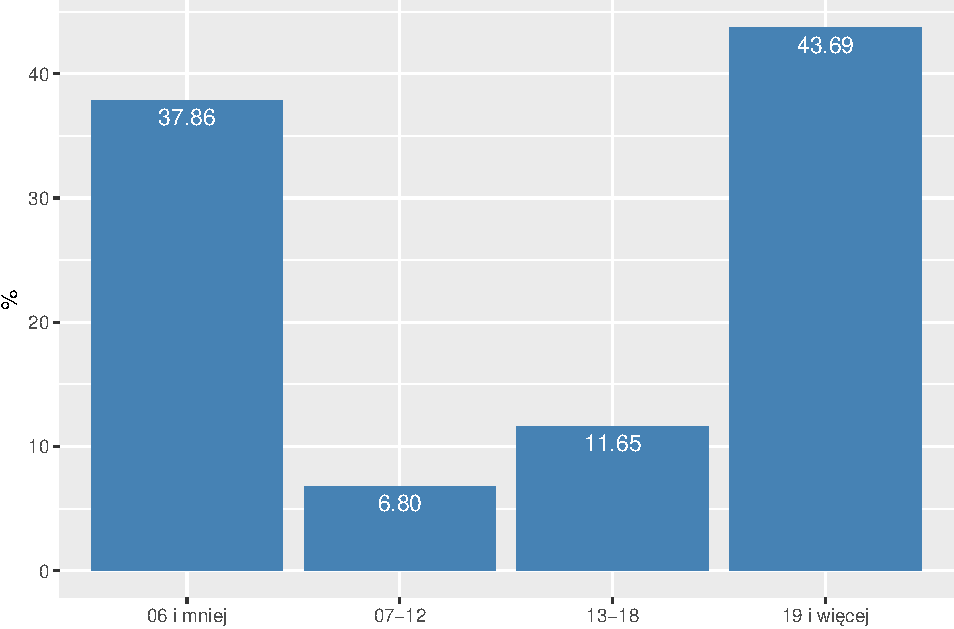
\includegraphics[width=0.85\linewidth]{_main_files/figure-latex/rysunek57-1} \caption{Studenci wg stażu pracy (\%)}\label{fig:rysunek57}
\end{figure}

\hypertarget{weryfikacja-hipotezy-1-1}{%
\subsection{Weryfikacja hipotezy 1}\label{weryfikacja-hipotezy-1-1}}

Rozkład studentów wg stanu psychicznego przedstawiono na wykresie \ref{fig:rysunek58}.

\begin{figure}
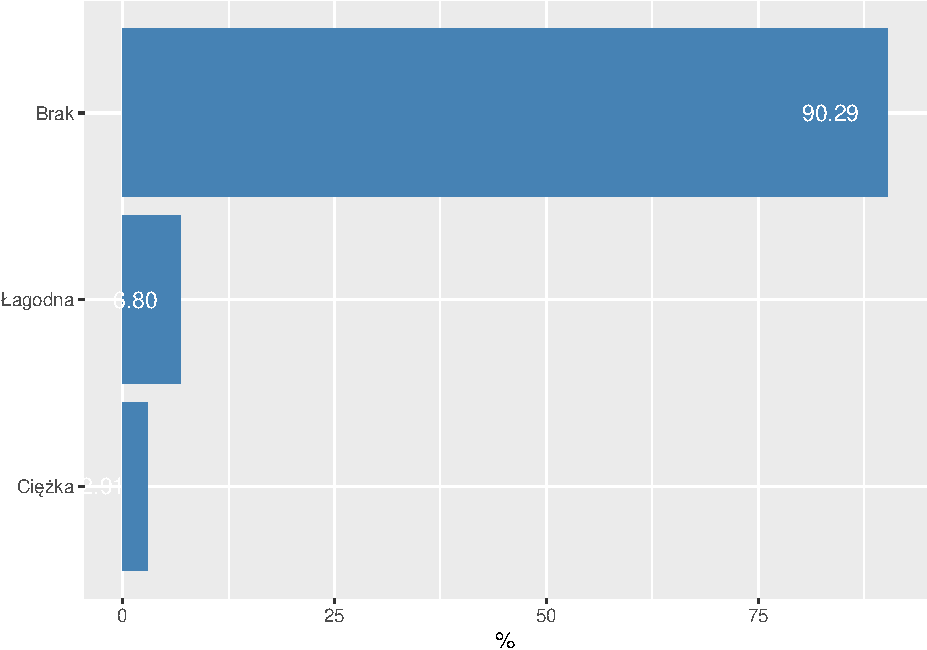
\includegraphics[width=0.85\linewidth]{_main_files/figure-latex/rysunek58-1} \caption{Studenci wg stanu psychicznego (\%)}\label{fig:rysunek58}
\end{figure}

Ciężką postać depresji wykazuje zaledwie 3\% studentów. Należy odrzucić hipotezę
że depresja stanowi poważny problem wśród studentów RM/PO PSW.

\hypertarget{weryfikacja-hipotez-24}{%
\subsection{Weryfikacja hipotez 2--4}\label{weryfikacja-hipotez-24}}

Aby móc zastosować metody tablicy wielodzielczej i testu chi-kwadrat
oryginalne wartości liczbowe depresji zamieniono
na skalę porządkową: 0--19 brak/łagodna depresja (Brak);
20--25 umiarkowana (Łagodna); 26--63 ciężka (Ciężka).

\hypertarget{depresja-a-pux142eux107}{%
\subsection{Depresja a płeć}\label{depresja-a-pux142eux107}}

Tablica wielodzielcza i test chi-kwadrat:

\begin{tabular}{lrr}
\toprule
  & K & M\\
\midrule
Brak & 64 & 29\\
Łagodna & 5 & 2\\
Ciężka & 2 & 1\\
\bottomrule
\end{tabular}

\begin{verbatim}
## 
##  Pearson's Chi-squared test
## 
## data:  dep.sex.f
## X-squared = 0,028134, df = 2, p-value = 0,986
\end{verbatim}

Nie stwierdzono zależności pomiędzy depresją a płcią (p = \text{0,986}).

\hypertarget{depresja-a-staux17c}{%
\subsection{Depresja a staż}\label{depresja-a-staux17c}}

Tablica wielodzielcza i test chi-kwadrat:

\begin{tabular}{lrrrr}
\toprule
  & 06 i mniej & 07-12 & 13-18 & 19 i więcej\\
\midrule
Brak & 36 & 6 & 9 & 42\\
Łagodna & 2 & 1 & 2 & 2\\
Ciężka & 1 & 0 & 1 & 1\\
\bottomrule
\end{tabular}

\begin{verbatim}
## 
##  Pearson's Chi-squared test
## 
## data:  dep.staz.f
## X-squared = 4,719, df = 6, p-value = 0,5803
\end{verbatim}

Nie stwierdzono zależności pomiędzy depresją a stażem pracy (p = \text{0,5803}).

Jeżeli depresję mierzymy na (oryginalnej) skali liczbowej
można zastosować test ANOVA lub Kruskala-Wallisa.

\begin{tabular}{lrrr}
\toprule
staż & średnia & mediana & n\\
\midrule
06 i mniej & 8,512821 & 7 & 39\\
07-12 & 7,857143 & 4 & 7\\
13-18 & 7,666667 & 3 & 12\\
19 i więcej & 8,533333 & 6 & 45\\
\bottomrule
\end{tabular}

Sprawdzamy czy rozkłady są normalne:

\begin{tabular}{lrr}
\toprule
staż & S-W & p\\
\midrule
06 i mniej & 0,9008198 & 0,0023292\\
07-12 & 0,8565271 & 0,1408865\\
13-18 & 0,7596157 & 0,0033736\\
19 i więcej & 0,6780397 & 0,0000000\\
\bottomrule
\end{tabular}

Nie są. Należy zastosować test Kruskala-Wallisa:

\begin{verbatim}
## [1] 0,678923
\end{verbatim}

Wynik jest ten sam (brak zależności). Nie ma
różnicy w poziomie depresji wśród pracowników o różnym stażu pracy.

\hypertarget{depresja-a-rodzaj-miejsca-pracy}{%
\subsection{Depresja a rodzaj miejsca pracy}\label{depresja-a-rodzaj-miejsca-pracy}}

Tablica wielodzielcza i test chi-kwadrat:

\begin{tabular}{lrr}
\toprule
  & Przychodnia & Szpital\\
\midrule
Brak & 12 & 81\\
Łagodna & 0 & 7\\
Ciężka & 0 & 3\\
\bottomrule
\end{tabular}

\begin{verbatim}
## 
##  Pearson's Chi-squared test
## 
## data:  dep.praca.f
## X-squared = 1,4605, df = 2, p-value = 0,4818
\end{verbatim}

Nie stwierdzono zależności pomiędzy depresją
a miejscem pracy (p = \text{0,4818}).

Jeżeli depresję mierzymy na skali liczbowej można zastosować test Welcha lub test Manna-Whitneya.

\begin{tabular}{lrrr}
\toprule
m-pracy & średnia & mediana & n\\
\midrule
Przychodnia & 7,833333 & 7 & 12\\
Szpital & 8,450549 & 6 & 91\\
\bottomrule
\end{tabular}

Sprawdzamy czy rozkłady są normalne:

\begin{tabular}{lrr}
\toprule
m-pracy. & S-W & p\\
\midrule
Przychodnia & 0,9256178 & 0,3359655\\
Szpital & 0,7865090 & 0,0000000\\
\bottomrule
\end{tabular}

Nie są. Należy zastosować test Manna-Whitneya:

\begin{verbatim}
## $p.value
## [1] 0,8528214
\end{verbatim}

Wynik jest ten sam (brak zależności). Nie ma
różnicy w poziomie depresji wśród pracowników szpitali i przychodni.

\hypertarget{wnioski-1}{%
\subsection{Wnioski}\label{wnioski-1}}

\begin{itemize}
\item
  Depresja nie jest istotnym problemem wśród studentów PSW.
\item
  Nie ma związku pomiędzy depresją a stażem, płcią i miejscem pracy.
\end{itemize}

\hypertarget{satysfakcja-przywiux105zanie-i-zamiar-odejux15bcia}{%
\section{Satysfakcja, przywiązanie i zamiar odejścia}\label{satysfakcja-przywiux105zanie-i-zamiar-odejux15bcia}}

\hypertarget{cel-2}{%
\subsection{Cel}\label{cel-2}}

Czy satysfakcja z pracy, satysfakcja z wynagrodzenia,
konflikt personalny ze współpracownikami oraz
konflikt personalny z przełożonym warunkują
przywiązanie do miejsca
pracy oraz zamiar zmiany miejsca pracy (zamiar odejścia) w środowisku
pielęgniarek/pielęgniarzy.

\textbf{Postawiono następujące hipotezy badawcze}:

\begin{enumerate}
\def\labelenumi{\arabic{enumi}.}
\item
  Wysoka satysfakcja z pracy oraz satysfakcja z wynagrodzenia zmniejszają
  zamiar zmiany miejsca pracy.
\item
  Konflikt personalny zwiększa zamiar zmiany miejsca pracy.
\item
  Duże przywiązanie do miejsca pracy zmniejsza zamiar zmiany miejsca pracy.
\item
  Zamiar zmiany miejsca pracy zależy od płci i stażu pracy.
\item
  Praca na oddziale ratunkowym lub intensywnej terapii zwiększa
  zamiar zmiany miejsca pracy
\item
  Zmianę miejsca pracy zależy od satysfakcji z pracy, satysfakcji z wynagrodzenia,
  konfliktu personalnego,
  przywiązania do miejsca pracy,
  pracy na oddziale ratunkowym lub intensywnej terapii,
  stażu i poziom satysfakcji.
\end{enumerate}

\hypertarget{metoda-2}{%
\subsection{Metoda}\label{metoda-2}}

Badanie ankietowe wśród studentów PSW przeprowadzono w 2023/2024 roku.
Zamiar zmiany pracy (ZZP),
przywiązanie do miejsca pracy (przywiązanie organizacyjne PO),
satysfakcja z pracy (SP),
satysfakcja z wynagrodzenia (SW),
konflikt personalny ze współpracownikami (KPW)
oraz konflikt personalny z przełożonym (KPP) były mierzone za pomocą
stosownych skal pomiarowych. Ankietowani byli także pytani
o płeć, staż oraz
czy pracują na oddziale ratunkowym/intensywnej terapii (\texttt{roddzial}).

\hypertarget{zastosowane-metody-statystyczne-2}{%
\subsection{Zastosowane metody statystyczne}\label{zastosowane-metody-statystyczne-2}}

\begin{itemize}
\item
  Do weryfikacji hipotez 1--5 wykorzystano model regresji liniowej.
\item
  Do weryfikacji hipotezy 6 wykorzystano model regresji logistycznej.
\end{itemize}

\hypertarget{wyniki}{%
\subsection{Wyniki}\label{wyniki}}

Pomniemy część opisową wyników żeby się nie powtarzać i przejdziemy
od razu do weryfikacji hipotez 1--6.

Macierz korelacji dla zmiennych \texttt{zzp}, \texttt{sp}, \texttt{sw}, \texttt{kpw}, \texttt{kpp} oraz \texttt{po}:

\begin{verbatim}
##          zzp      sp      sw     kpw     kpp      po    staz
## zzp   1,0000 -0,5095 -0,1644  0,3245  0,3796 -0,3325  0,0666
## sp   -0,5095  1,0000  0,2815 -0,1041 -0,3446  0,3103 -0,0918
## sw   -0,1644  0,2815  1,0000 -0,4524  0,0163  0,1801 -0,1994
## kpw   0,3245 -0,1041 -0,4524  1,0000  0,4234 -0,1339  0,0030
## kpp   0,3796 -0,3446  0,0163  0,4234  1,0000 -0,3380 -0,1015
## po   -0,3325  0,3103  0,1801 -0,1339 -0,3380  1,0000  0,2808
## staz  0,0666 -0,0918 -0,1994  0,0030 -0,1015  0,2808  1,0000
\end{verbatim}

Można zaobserwować wiele wysokich wartości współczynnika korelacji
(\texttt{zpp}/\texttt{sp}, \texttt{zpp}/\texttt{kpw}, \texttt{pp}/\texttt{kpp}), ale też niektóre są beznadziejnie niskie (np. \texttt{zpp}/\texttt{staż}).

\textbf{Regresja liniowa}

Zakładamy, że \texttt{zzp} jest objaśniana przez \texttt{sp}, \texttt{sw}, \texttt{kpw}, \texttt{kpp}, \texttt{po}, \texttt{staz}, \texttt{plec} oraz \texttt{roddzial}.
(Odważnie dołączamy \texttt{staz} mimo że w świetle analizy macierzy korelacji raczej nie jest to dobry pomysł.)
Oszacowanie tego modelu daje następujące wyniki:

\begin{tabular}{lrrrrrl}
\toprule
Zmienna & B & SE & z & p & Beta & CI\\
\midrule
(Intercept) & 13,035 & 3,706 & 3,517 & 0,001 & NA & 5,57 20,50\\
sp & -1,099 & 0,331 & -3,325 & 0,002 & -0,48 & -1,76 -0,43\\
sw & 0,124 & 0,115 & 1,075 & 0,288 & 0,16 & -0,11  0,36\\
kpw & 0,778 & 0,376 & 2,068 & 0,044 & 0,31 & 0,02  1,54\\
kpp & 0,032 & 0,235 & 0,137 & 0,891 & 0,02 & -0,44  0,50\\
\addlinespace
po & -0,040 & 0,026 & -1,545 & 0,129 & -0,21 & -0,09  0,01\\
staz & 0,045 & 0,047 & 0,953 & 0,346 & 0,13 & -0,05  0,14\\
plecM & 0,624 & 2,437 & 0,256 & 0,799 & 0,04 & -4,28  5,53\\
roddzialtak & 1,138 & 0,896 & 1,270 & 0,211 & 0,15 & -0,67  2,94\\
\bottomrule
\end{tabular}

Współczynnik zbieżności wynosi \text{40,85}\%.
Tylko dwie zmienne \texttt{sp} oraz \texttt{kpw} okazały się istotne.

Stosując metodę regresji krokowej usuwamy iteracyjnie (jedną na raz) wszystkie zmienne
nieistotne. Kolejno należało wyeliminować \texttt{sw}, \texttt{kpp}, \texttt{po}, \texttt{staz}, \texttt{plec} oraz \texttt{roddzial}.
W modelu ostatecznym \texttt{zzp} jest objaśniana przez \texttt{sp} oraz \texttt{kpw}:

\begin{tabular}{lrrrrrl}
\toprule
Zmienna & B & SE & z & p & Beta & CI\\
\midrule
(Intercept) & 13,987 & 2,969 & 4,710 & 0,000 & NA & 8,03 19,95\\
sp & -1,112 & 0,263 & -4,226 & 0,000 & -0,48 & -1,64 -0,58\\
kpw & 0,682 & 0,283 & 2,412 & 0,019 & 0,27 & 0,11  1,25\\
\bottomrule
\end{tabular}

Współczynnik zbieżności wynosi \text{33,41}\%.
Satysfakcja jest większym predyktorem zamiaru zmiany pracy (kolumna Beta).

\textbf{Regresja logistyczna}

Żeby zademonstrować przykład wykorzystania regresji logistycznej przyjmijmy, że jak ktoś bardzo chce
zmienić pracę to ją zmieni.
Niech to \textbf{bardzo chce} będzie wtedy kiedy wartość \texttt{zzp} wynosi co najmniej 12.
Zmienną \texttt{zzp} należy w tym celu przekodować na zmienną dwuwartościową (nazwijmy ją \texttt{zp}), która
przyjmuje wartość 0 jeżeli \texttt{zzp} jest większe
równe od 12 lub wartość 1 jeżeli \texttt{zzp} jest mniejsze od 12.
Model nie objaśnia teraz zależności pomiędzy zamiarem, ale prognozuje
zmianę miejsca pracy (zmieni=0, nie zmieni=1).

Zakładamy, że \texttt{zp}, podobnie jak w przypadku zamiaru,
jest objaśniana przez \texttt{sp}, \texttt{sw}, \texttt{kpw}, \texttt{kpp}, \texttt{po}, \texttt{staz}, \texttt{plec} oraz \texttt{roddzial}.

\begin{tabular}{lrrrrrl}
\toprule
Parametr & Ocena & SE & z & p & OR & CI\\
\midrule
(Intercept) & -4,702 & 4,599 & -1,022 & 0,307 & 0,01 & 0,00 82,27\\
sp & 1,082 & 0,480 & 2,254 & 0,024 & 2,95 & 1,30  9,15\\
sw & -0,082 & 0,143 & -0,577 & 0,564 & 0,92 & 0,68  1,22\\
kpw & -0,415 & 0,410 & -1,013 & 0,311 & 0,66 & 0,28  1,51\\
kpp & 0,154 & 0,386 & 0,399 & 0,690 & 1,17 & 0,62  2,53\\
\addlinespace
po & 0,037 & 0,036 & 1,028 & 0,304 & 1,04 & 0,97  1,13\\
staz & -0,107 & 0,071 & -1,512 & 0,130 & 0,90 & 0,76  1,02\\
plecM & 13,102 & 2596,962 & 0,005 & 0,996 & 489784,87 & 0,00    NA\\
roddzialtak & -1,817 & 1,074 & -1,692 & 0,091 & 0,16 & 0,02  1,31\\
\bottomrule
\end{tabular}

Wartości większości współczynników okazały się nieistotne. Mówiąc konkretniej na poziomie
istotności 0,05 tylko \texttt{sp} jest istotna (\texttt{roddzialtak} jest także istotny ale na poziomie 0,1).

Postępując podobnie jak w przypadku „normalnej'' regresji eliminujemy
iteracyjnie wszystkie zmienne nieistotne ostatecznie dochodząc
do modelu w którym odejście z pracy objaśnia tylko satysfakcja:

\begin{tabular}{lrrrrrl}
\toprule
Parametr & Ocena & SE & z & p & OR & CI\\
\midrule
(Intercept) & -5,448 & 2,460 & -2,215 & 0,027 & 0,00 & 0,00 0,36\\
sp & 0,803 & 0,283 & 2,838 & 0,005 & 2,23 & 1,35 4,26\\
\bottomrule
\end{tabular}

Macierz pomyłek:

\begin{verbatim}
##         zp
## Prognoza  0  1
##        0  3  1
##        1  6 45
\end{verbatim}

Stąd: czułość \text{0,98}; swoistość \text{0,33}.

Krzywą ROC przedstawiono na rysunku:

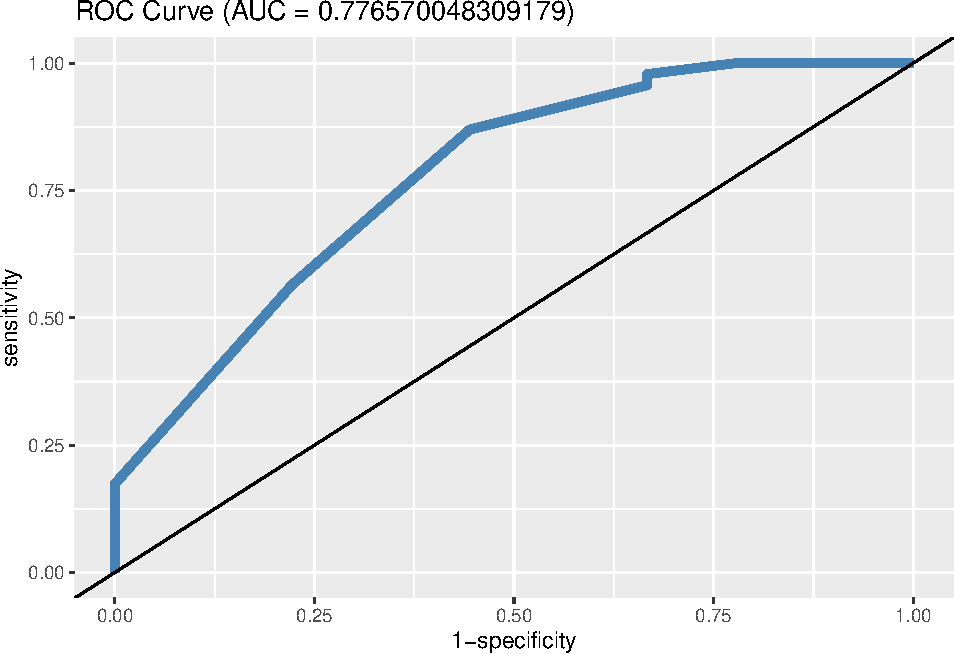
\includegraphics[width=0.7\linewidth]{_main_files/figure-latex/unnamed-chunk-113-1}

\hypertarget{wnioski-2}{%
\subsection{Wnioski}\label{wnioski-2}}

\begin{itemize}
\item
  Satysfakcja jest większym predyktorem zamiaru zmiany pracy niż konflikt personalny
  ze współpracownikami.
  Pozostałe czynniki okazały się nieistotne (hipotezy 1--5).
\item
  Satysfakcja jest jedynym czynnikiem istotnie wpływającym na zmianę miejsca pracy.
  Pozostałe czynniki okazały się nieistotne (hipoteza 6).
\end{itemize}

\hypertarget{formularze-ankiet}{%
\section{Formularze ankiet}\label{formularze-ankiet}}

\hypertarget{skala-depresji-becka}{%
\subsection{Skala Depresji Becka}\label{skala-depresji-becka}}

\textbf{Pytania}

Pytanie 1

\begin{enumerate}
\def\labelenumi{\arabic{enumi}.}
\setcounter{enumi}{-1}
\tightlist
\item
  Nie jestem smutny ani przygnębiony.
\item
  Odczuwam często smutek, przygnębienie
\item
  Przeżywam stale smutek, przygnębienie i nie mogę uwolnić się od tych przeżyć.
\item
  Jestem stale tak smutny i nieszczęśliwy, że jest to nie do wytrzymania.
\end{enumerate}

Pytanie 2

\begin{enumerate}
\def\labelenumi{\arabic{enumi}.}
\setcounter{enumi}{-1}
\tightlist
\item
  Nie przejmuję się zbytnio przyszłością.
\item
  Często martwię się o przyszłość.
\item
  Obawiam się, że w przyszłości nic dobrego mnie nie czeka.
\item
  Czuję, że przyszłość jest beznadziejna i nic tego nie zmieni.
\end{enumerate}

Pytanie 3

\begin{enumerate}
\def\labelenumi{\arabic{enumi}.}
\setcounter{enumi}{-1}
\tightlist
\item
  Sądzę, że nie popełniam większych zaniedbań.
\item
  Sądzę, że czynię więcej zaniedbań niż inni.
\item
  Kiedy spoglądam na to, co robiłem, widzę mnóstwo błędów i zaniedbań.
\item
  Jestem zupełnie niewydolny i wszystko robię źle.
\end{enumerate}

Pytanie 4

\begin{enumerate}
\def\labelenumi{\arabic{enumi}.}
\setcounter{enumi}{-1}
\tightlist
\item
  To, co robię, sprawia mi przyjemność.
\item
  Nie cieszy mnie to, co robię.
\item
  Nic mi teraz nie daje prawdziwego zadowolenia.
\item
  Nie potrafię przeżywać zadowolenia i przyjemności; wszystko mnie nuży.
\end{enumerate}

Pytanie 5

\begin{enumerate}
\def\labelenumi{\arabic{enumi}.}
\setcounter{enumi}{-1}
\tightlist
\item
  Nie czuję się winnym ani wobec siebie, ani wobec innych.
\item
  Dość często miewam wyrzuty sumienia.
\item
  Często czuję, że zawiniłem.
\item
  Stale czuję się winny.
\end{enumerate}

Pytanie 6

\begin{enumerate}
\def\labelenumi{\arabic{enumi}.}
\setcounter{enumi}{-1}
\tightlist
\item
  Sądzę, że nie zasługuję na karę
\item
  Sądzę, że zasługuję na karę
\item
  Spodziewam się ukarania
\item
  Wiem, że jestem karany (lub ukarany)
\end{enumerate}

Pytanie 7

\begin{enumerate}
\def\labelenumi{\arabic{enumi}.}
\setcounter{enumi}{-1}
\tightlist
\item
  Jestem z siebie zadowolony
\item
  Nie jestem z siebie zadowolony
\item
  Czuję do siebie niechęć
\item
  Nienawidzę siebie
\end{enumerate}

Pytanie 8

\begin{enumerate}
\def\labelenumi{\arabic{enumi}.}
\setcounter{enumi}{-1}
\tightlist
\item
  Nie czuję się gorszy od innych ludzi
\item
  Zarzucam sobie, że jestem nieudolny i popełniam błędy
\item
  Stale potępiam siebie za popełnione błędy
\item
  Winię siebie za wszelkie zło, które istnieje
\end{enumerate}

Pytanie 9

\begin{enumerate}
\def\labelenumi{\arabic{enumi}.}
\setcounter{enumi}{-1}
\tightlist
\item
  Nie myślę o odebraniu sobie życia
\item
  Myślę o samobójstwie -- ale nie mógłbym tego dokonać
\item
  Pragnę odebrać sobie życie
\item
  Popełnię samobójstwo, jak będzie odpowiednia sposobność
\end{enumerate}

Pytanie 10

\begin{enumerate}
\def\labelenumi{\arabic{enumi}.}
\setcounter{enumi}{-1}
\tightlist
\item
  Nie płaczę częściej niż zwykle
\item
  Płaczę częściej niż dawniej
\item
  Ciągle chce mi się płakać
\item
  Chciałbym płakać, lecz nie jestem w stanie
\end{enumerate}

Pytanie 11

\begin{enumerate}
\def\labelenumi{\arabic{enumi}.}
\setcounter{enumi}{-1}
\tightlist
\item
  Nie jestem bardziej podenerwowany niż dawniej
\item
  Jestem bardziej nerwowy i przykry niż dawniej
\item
  Jestem stale zdenerwowany lub rozdrażniony
\item
  Wszystko, co dawniej mnie drażniło, stało się obojętne
\end{enumerate}

Pytanie 12

\begin{enumerate}
\def\labelenumi{\arabic{enumi}.}
\setcounter{enumi}{-1}
\tightlist
\item
  Ludzie interesują mnie jak dawniej
\item
  Interesuję się ludźmi mniej niż dawniej
\item
  Utraciłem większość zainteresowań innymi ludźmi
\item
  Utraciłem wszelkie zainteresowanie innymi ludźmi
\end{enumerate}

Pytanie 13

\begin{enumerate}
\def\labelenumi{\arabic{enumi}.}
\setcounter{enumi}{-1}
\tightlist
\item
  Decyzje podejmuję łatwo, tak jak dawniej
\item
  Częściej niż kiedyś odwlekam podjęcie decyzji
\item
  Mam dużo trudności z podjęciem decyzji
\item
  Nie jestem w stanie podjąć żadnej decyzji
\end{enumerate}

Pytanie 14

\begin{enumerate}
\def\labelenumi{\arabic{enumi}.}
\setcounter{enumi}{-1}
\tightlist
\item
  Sądzę, że wyglądam nie gorzej niż dawniej
\item
  Martwię się tym, że wyglądam staro i nieatrakcyjnie
\item
  Czuję, że wyglądam coraz gorzej
\item
  Jestem przekonany, że wyglądam okropnie i odpychająco
\end{enumerate}

Pytanie 15

\begin{enumerate}
\def\labelenumi{\arabic{enumi}.}
\setcounter{enumi}{-1}
\tightlist
\item
  Mogę pracować jak dawniej
\item
  Z trudem rozpoczynam każdą czynność
\item
  Z wielkim wysiłkiem zmuszam się do zrobienia czegokolwiek
\item
  Nie jestem w stanie nic zrobić
\end{enumerate}

Pytanie 16

\begin{enumerate}
\def\labelenumi{\arabic{enumi}.}
\setcounter{enumi}{-1}
\tightlist
\item
  Sypiam dobrze, jak zwykle
\item
  Sypiam gorzej niż dawniej
\item
  Rano budzę się 1--2 godziny za wcześnie i trudno jest mi ponownie usnąć
\item
  Budzę się kilka godzin za wcześnie i nie mogę usnąć
\end{enumerate}

Pytanie 17

\begin{enumerate}
\def\labelenumi{\arabic{enumi}.}
\setcounter{enumi}{-1}
\tightlist
\item
  Nie męczę się bardziej niż dawniej
\item
  Męczę się znacznie łatwiej niż poprzednio.
\item
  Męczę się wszystkim, co robię.
\item
  Jestem zbyt zmęczony, aby cokolwiek robić.
\end{enumerate}

Pytanie 18

\begin{enumerate}
\def\labelenumi{\arabic{enumi}.}
\setcounter{enumi}{-1}
\tightlist
\item
  Mam apetyt nie gorszy niż dawniej
\item
  Mam trochę gorszy apetyt
\item
  Apetyt mam wyraźnie gorszy
\item
  Nie mam w ogóle apetytu
\end{enumerate}

Pytanie 19

\begin{enumerate}
\def\labelenumi{\arabic{enumi}.}
\setcounter{enumi}{-1}
\tightlist
\item
  Nie tracę na wadze (w okresie ostatniego miesiąca)
\item
  Straciłem na wadze więcej niż 2 kg
\item
  Straciłem na wadze więcej niż 4 kg
\item
  Straciłem na wadze więcej niż 6 kg
\end{enumerate}

Pytanie 20

\begin{enumerate}
\def\labelenumi{\arabic{enumi}.}
\setcounter{enumi}{-1}
\tightlist
\item
  Nie martwię się o swoje zdrowie bardziej niż zawsze
\item
  Martwię się swoimi dolegliwościami, mam rozstrój żołądka, zaparcie, bóle
\item
  Stan mojego zdrowia bardzo mnie martwi, często o tym myślę
\item
  Tak bardzo martwię się o swoje zdrowie, że nie mogę o niczym innym myśleć
\end{enumerate}

Pytanie 21

\begin{enumerate}
\def\labelenumi{\arabic{enumi}.}
\setcounter{enumi}{-1}
\tightlist
\item
  Moje zainteresowania seksualne nie uległy zmianom
\item
  Jestem mniej zainteresowany sprawami płci (seksu)
\item
  Problemy płciowe wyraźnie mniej mnie interesują
\item
  Utraciłem wszelkie zainteresowanie sprawami seksu
\end{enumerate}

\textbf{Treść pytań} (nie prezentowana ankietowanym):
Odczuwanie smutku i przygnębienia (1),
Martwienie się o przyszłość (2),
Uważasz, że zaniedbujesz swoje obowiązki? (3),
Jesteś zadowolony z siebie? (4),
Czy często masz poczucie winy? (5),
Czy zasługujesz na karę? (6),
Zadowolenie z siebie (7),
Czy czujesz się gorszy od innych? (8),
Czy masz myśli samobójcze? (9),
Często chce Ci się płakać? (10),
Jesteś ostatnio bardziej nerwowy i rozdrażniony? (11),
Czy zmieniło się coś w Twoim zainteresowaniu innymi ludźmi? (12),
Czy ostatnio miewasz większe problemy z podejmowaniem różnych decyzji? (13),
Czy uważasz, że wyglądasz gorzej i mniej atrakcyjnie niż kiedyś? (14),
Czy masz większe trudności z wykonywaniem różnych prac i zadań? (15),
Masz kłopoty ze snem? (16),
Czy męczysz się bardziej niż zwykle? (17),
Czy masz kłopoty z apetytem? (18),
W ciągu ostatniego miesiąca nie stosowałem diety, aby schudnąć,
lecz straciłem na wadze (19),
Czy ostatnio bardziej martwisz się swoim stanem zdrowia? (20),
Czy masz kłopoty z potencją? (21).

\textbf{Interpretacja wyników}

\begin{longtable}[]{@{}ll@{}}
\toprule\noalign{}
Punkty & Depresja \\
\midrule\noalign{}
\endhead
\bottomrule\noalign{}
\endlastfoot
0--11 & Brak \\
12--19 & Łagodna \\
20--25 & Umiarkowana \\
26--63 & Ciężka \\
\end{longtable}

\textbf{Źródło}:
\url{https://psychiatra.bydgoszcz.eu/publikacje-dla-pacjenta/depresja/skala-depresji-becka/}
oraz
\url{http://centrum-psychologiczne.com/files/files/Skala_Depresji_Becka_word.pdf}

\hypertarget{ankieta-na-temat-szkodliwoux15bci-palenia}{%
\subsection{Ankieta na temat szkodliwości palenia}\label{ankieta-na-temat-szkodliwoux15bci-palenia}}

Poziom wiedzy personelu pielęgniarskiego na temat szkodliwości palenia tytoniu

\textbf{Pytania}

\begin{enumerate}
\def\labelenumi{\arabic{enumi}.}
\item
  Płeć
  □ Kobieta
  □ Mężczyzna
\item
  Wiek
\item
  Pochodzenie
  □ wieś
  □ Miasto do 20 tys. mieszkańców
  □ Miasto powyżej 20 tyś mieszkańców
\item
  Wykształcenie
  □ Średnie medyczne
  □ Licencjat pielęgniarstwa
  □ Magister pielęgniarstwa
  □ Inne wyższe
\item
  Staż pracy
  □ Mniej niż rok
  □ 1-10 lat
  □ 10-15 lat
  □ Więcej niż 15 lat
\item
  Miejsce pracy
  □ Oddział zabiegowy
  □ Oddział zachowawczy
  □ Przychodnia/poradnia
\item
  Czy kiedykolwiek paliłeś/aś papierosy?
  □ Paliłem/łam
  □ W dalszym ciągu palę
  □ Nigdy nie paliłem/am
\item
  Od ilu lat palisz?
  □ Nie palę/Nie dotyczy
  □ Mniej niż rok
  □ 1-10 lat
  □ 11-15 lat
  □ Więcej niż 15 l
\item
  Czy zdarza Ci się palić w miejscu pracy?
  □ Tak
  □ Nie
  □ Nie dotyczy
\item
  Czy próbowałeś kiedykolwiek rzucić palenie?
  □ Tak, udało się
  □ Tak, ale wróciłem/am do nałogu
  □ Nie
  □ Nie dotyczy
\item
  Czy paląc przyznajesz się do uzależnienia
  □ Tak
  □ Nie
  □ Nie dotyczy
\item
  Uważasz, że bardziej szkodliwe dla zdrowia jest:
  □ Palenie czynne - dym tytoniowy wdychany bezpośrednio przez palacza
  □ Palenie bierne-boczny strumień dymu
  ☒ Każda forma kontaktu z dymem jest równie szkodliwa
  □ Nie wiem/Nie mam zdania
\item
  Czy uważasz,że przepisy prawa powinny zabraniać palenia w obecności dzieci
  poniżej 15 roku życia?
  □ Tak
  □ Nie
  □ Nie wiem/nie mam zdania
\item
  Czy przerwa na papierosa pomaga Ci w sytuacjach stresowych?
  □ Tak
  □ Nie
  □ Nie dotyczy
\item
  Czy palenie nikotyny sprawia Ci przyjemność?
  □ Tak
  □ Nie
  □ Nie dotyczy
\item
  Jakie według Ciebie choroby układu oddechowego mogą być spowodowane
  bezpośrednio przez palenie papierosów?(wielokrotnego)
  ☒ Przewlekła obturacyjna choroba płuc
  ☒ Astma oskrzelowa
  ☒ Alergie wziewne
  □ Gruźlica
  □ Zapalenie płuc
  ☒ Przewlekłe zapalenie oskrzeli
  ☒ Infekcje dróg oddechowych
  □ Palenie nie powoduje chorób układu oddechowego
  □ Nie wiem
\item
  Jakie według Ciebie choroby kardiologiczne mogą być spowodowane
  bezpośrednio przez palenie papierosów? (wielokrotnego)
  ☒ Nadciśnienie tętnicze krwi
  ☒ Zawał mięśnia sercowego
  ☒ Udar mózgu
  ☒ Choroba niedokrwienna serca
  ☒ Miażdżyca tętnic obwodowych
  ☒ Zaburzenie rytmu serca
  ☒ Choroba Buergera
  □ Hipercholesterolemia
  □ Tętniak aorty
  □ Palenie nie powoduje chorób kardiologicznych
\item
  Czy palenie papierosów powoduje choroby układu pokarmowego?
  ☒ Tak
  □ Nie
  □ Nie wiem
\item
  Jaki według Ciebie ma wpływ palenie papierosów na narządy zmysłów? (wielokrotnego)
  ☒ Upośledza węch i smak
  ☒ Powoduje podrażnienie spojówek
  ☒ Obniża apetyt
  ☒ Niszczy struny głosowe
  ☒ Zmniejsza ostrość wzroku
  □ Palenie nie ma negatywnego wpływu na narządy zmysłu.
\item
  Jak oceniasz swoją wiedzę na temat palenia papierosów i jego wpływu na zdrowie człowieka?
  □ Bardzo dobrze
  □ Dobrze
  □ Przeciętnie
  □ Źle
\item
  Czy wzorce sięgania po tytoń wyniosłaś/wyniosłeś z domu rodzinnego
  □ Tak
  □ Nie
  □ Nie dotyczy
\end{enumerate}

(Prawidłowe odpowiedzi zaznaczono ☒)

\textbf{Źródło}: Na podstawie ankiety z pracy Izabeli Marendowskiej
\emph{Ocena poziomu wiedzy pielęgniarek na
temat szkodliwości palenia papierosów} (promotor: dr Marzena Barton);
Kwidzyn 2022.

\hypertarget{ankieta-satysfakcja-przywiux105zanie-i-zamiar-odejux15bcia}{%
\subsection{Ankieta satysfakcja, przywiązanie i zamiar odejścia}\label{ankieta-satysfakcja-przywiux105zanie-i-zamiar-odejux15bcia}}

\textbf{Zamiar zmiany pracy/ZZP}

(Zdecydowanie się nie zgadzam/Nie zgadzam się/Trudno powiedzieć/Zgadzam się/Zdecydowanie się zgadzam.)

\begin{enumerate}
\def\labelenumi{\arabic{enumi}.}
\tightlist
\item
  Często poważnie rozważam odejście z obecnej pracy
\item
  Zamierzam rzucić obecną pracę
\item
  Zacząłem szukać innej pracy
\end{enumerate}

\textbf{Satysfakcja z pracy/SP}

(Zdecydowanie się nie zgadzam/Nie zgadzam się/Trudno powiedzieć/Zgadzam się/Zdecydowanie się zgadzam.)

\begin{enumerate}
\def\labelenumi{\arabic{enumi}.}
\setcounter{enumi}{3}
\tightlist
\item
  Ogólnie rzecz biorąc nie lubię swojej pracy
\item
  Ogólnie rzecz biorąc jestem zadowolony ze swojej pracy
\item
  Ogólnie rzecz biorąc, lubię tu pracować
\end{enumerate}

\textbf{Satysfakcja z pracy/SSP/alternatywna skala}

(Zdecydowanie się nie zgadzam/Nie zgadzam się/Trudno powiedzieć/Zgadzam się/Zdecydowanie się zgadzam.)

\begin{enumerate}
\def\labelenumi{\arabic{enumi}.}
\setcounter{enumi}{6}
\tightlist
\item
  Pod bardzo wieloma względami moja praca bliska jest ideału
\item
  Mam świetne warunki pracy
\item
  Jestem zadowolony z pracy
\item
  Jak dotąd w pracy udawało mi się osiągać to, czego chciałem
\item
  Gdybym miał decydować raz jeszcze, wybrałbym tę samą pracę
\end{enumerate}

\textbf{Satysfakcja z wynagrodzenia/SW}

(Zdecydowanie niesatysfakcjonująca-Niesatysfakcjonująca-TP-Satysfakcjonująca-Zdecydowanie niesatysfakcjonująca.)

\begin{enumerate}
\def\labelenumi{\arabic{enumi}.}
\setcounter{enumi}{11}
\tightlist
\item
  Moja pensja na rękę jest
\item
  Wielkość mojej obecnej pensji jest
\item
  Moje obecne wynagrodzenie jest
\item
  Poziom mojego łącznego wynagrodzenia jest
\end{enumerate}

\textbf{Konflikt ze współpracownikami/KPW}

(Raz na miesiąc lub mniej/1--2 razy w miesiącu/1--2 razy w tygodniu/1--2 razy dziennie/wiele razy dziennie.)

\begin{enumerate}
\def\labelenumi{\arabic{enumi}.}
\setcounter{enumi}{15}
\tightlist
\item
  Jak często w pracy kłócisz się z innymi osobami?
\item
  Jak często inni ludzie krzyczą na Ciebie w pracy?
\item
  Jak często ludzie są wobec Ciebie niemili w pracy?
\item
  Jak często inni ludzie robią Ci nieprzyjemne rzeczy w pracy?
\end{enumerate}

\textbf{Konflikt z przełożonym/KPP}

(Raz na miesiąc lub mniej/1--2 razy w miesiącu/1--2 razy w tygodniu/1--2 razy dziennie/wiele razy dziennie.)

\begin{enumerate}
\def\labelenumi{\arabic{enumi}.}
\setcounter{enumi}{19}
\tightlist
\item
  Jak często w pracy kłócisz się z przełożonym?
\item
  Jak często twój przełożony krzyczy na ciebie?
\item
  Jak często twój przełożony jest niemiły w pracy?
\item
  Jak często Twój przełożony robi ci nieprzyjemne rzeczy w pracy?
\end{enumerate}

\textbf{Przywiązanie do ogranizacji/PO} (\texttt{PO-1}--\texttt{PO-18}), składające się z następujących aspektów:
przywiązanie afektywne (\texttt{PO-1}--\texttt{PO-6}), przywiązanie normatywne (\texttt{PO-7}--\texttt{PO-12}),
przywiązanie trwania (\texttt{PO-13}--\texttt{PO-18}).

(Zdecydowanie się nie zgadzam/nie zgadzam się/raczej się nie zgadzam/
trudno powiedzieć/raczej się zgadzam/zgadzam się/zdecydowanie się zgadzam.)

\begin{enumerate}
\def\labelenumi{\arabic{enumi}.}
\setcounter{enumi}{23}
\tightlist
\item
  Zakład pracy, w której pracuję ma dla mnie duże znaczenie osobiste. (PO-2)
\item
  Czułbym się winny, gdybym teraz odszedł z mojego zakładu pracy (PO-18)
  26 .Zbyt wiele straciłbym w moim życiu, decydując się teraz na odejście z mojego zakładu pracy (PO-9)
\item
  Mogę powiedzieć, że czuję się w moim zakładzie pracy jak w rodzinie (PO-5)
\item
  Gdybym dostał ofertę lepszej pracy, czułbym się nie w porządku odchodząc z mojego zakładu pracy (PO-14)
\item
  Byłbym bardzo zadowolony gdybym do emerytury mógł pracować w moim zakładzie pracy (PO-11)
\item
  Wiele zawdzięczam mojemu zakładowi pracy (PO-4)
\item
  Jednym z głównych powodów, dla których wciąż pracuję
  w tym zakładzie pracy jest wiara w znaczenie lojalności\\
  dająca mi poczucie moralnego obowiązku pozostania (PO-16)
\item
  Czuje, że problemy mojego zakładu pracy są rzeczywiście moimi własnymi problemami (PO-6)
\item
  Nie odszedłbym teraz z mojego zakładu pracy, ponieważ mam zobowiązania
  w stosunku do ludzi, którzy w niej pracują (PO-17)
\item
  Jedną z kilku negatywnych konsekwencji odejścia z mojego zakładu pracy
  mógłby być brak dostępnych możliwości zatrudnienia (PO-10)
\item
  Byłoby mi bardzo ciężko odejść teraz z mojego zakładu pracy, nawet gdybym chciał (PO-3)
\item
  Ten zakład pracy zasługuje na to, żebym był wobec niego w porządku (PO-15)
\item
  Mam poczucie, że pozostanie w zakładzie pracy jest dla mnie koniecznością (PO-12)
\item
  Sprawia mi przyjemność, kiedy mogę porozmawiać o moim zakładzie pracy z ludźmi z zewnątrz (PO-1)
\item
  Sądzę, że odchodząc z mojego zakładu pracy, mam zbyt mało innych możliwości do wyboru (PO-8)
\item
  Nawet, gdyby to było dla mnie korzystne, nie czułbym się w porządku odchodząc
  teraz z mojego zakładu pracy (PO-13)
\item
  Lepiej było, kiedy ludzie większość swojego życia zawodowego wiązali z jedną firmą (PO-7)
\end{enumerate}

\textbf{Satysfakcja z pracy/SP0/skala jednopozycyjna}

\begin{enumerate}
\def\labelenumi{\arabic{enumi}.}
\setcounter{enumi}{41}
\tightlist
\item
  W jakim stopniu jesteś ogólnie zadowolony ze swojej pracy?
\end{enumerate}

(Bardzo niezadowolony/Niezadowolony/Trudno powiedzieć/Zadowolony/Bardzo zadowolony)

\textbf{Zamiar odejścia z pracy/ZZP0/skala jednopozycyjna}

(Nigdy/Rzadko/Czasami/Często/Bardzo często)

\begin{enumerate}
\def\labelenumi{\arabic{enumi}.}
\setcounter{enumi}{42}
\tightlist
\item
  Jak często poważnie rozważałeś odejście z obecnej pracy?
\end{enumerate}

\textbf{„Metryczka''}

\begin{enumerate}
\def\labelenumi{\arabic{enumi}.}
\setcounter{enumi}{43}
\tightlist
\item
  Płeć (K/M)
\item
  Rodzaj studiów
\item
  Staż łączny (lata pracy)
\item
  Ile razy zmieniałeś miejsce pracy?
\item
  Praca na oddziale ratunkowym lub intensywnej terapii (T/N)
\end{enumerate}

\textbf{Źródło:}
Liu Y i inni, \emph{Turnover intention and its associated factors among nurses: a multi-center cross-sectional study}
(Zamiar zmiany pracy oraz czynniki z nim związane wśród pielęgniarek: badanie przekrojowe.)
Front. Public Health 11:1141441 (2023)
\url{https://www.frontiersin.org/articles/10.3389/fpubh.2023.1141441/full}
oraz
Bańka A., Bazińska R., Wołowska A., \emph{Polska wersja Meyera i Allen Skali Przywiązania do Organizacji}, Czasopismo Psychologiczne 2002, nr 8 (1), s. 65--74.

\hypertarget{intro2jamovi}{%
\chapter{Praca z programem Jamovi}\label{intro2jamovi}}

Jak wspomniano w rozdziale 1, statystkę można uprawiać (tj. liczyć statystyki w drugim tego słowa znaczeniu :-))
wykorzystując różne programy. My zdecydowaliśmy się promować \textbf{Jamovi}, program
który naszym zdaniem jest najlepszym -- z punktu widzenia większości
studentów Nauk o Zdrowiu -- połączeniem ceny, możliwości, prostoty i łatwości nauki.

\hypertarget{podstawy-pracy-z-jamovi}{%
\section{Podstawy pracy z Jamovi}\label{podstawy-pracy-z-jamovi}}

Jamovi jest oprogramowaniem rozpowszechnianym na licencji typu \emph{Open Source},
a więc można go używać za darmo. Program jest dostępny ze strony
\url{https://www.jamovi.org/download.html}. Klikamy, ściągamy, uruchamiamy instalator.
Program jest dość duży, ale to nie jest aż tak wielki problem w czasach kiedy
pojemności dysków w domowym komputerze zaczynają się od 250 gigabajtów. Jest
też wersja Jamovi365, którą można się posługiwać w przeglądarce i wtedy nic nie trzeba
instalować na swoim komputerze.

W naszym podręczniku pokazujemy jak uprawiać statystykę z tradycyjną wersją Jamovi.
Po zainstalowaniu uruchamiamy program, którego ekran startowy wygląda jak
na rysunku \ref{fig:mainscreen}.

\begin{figure}
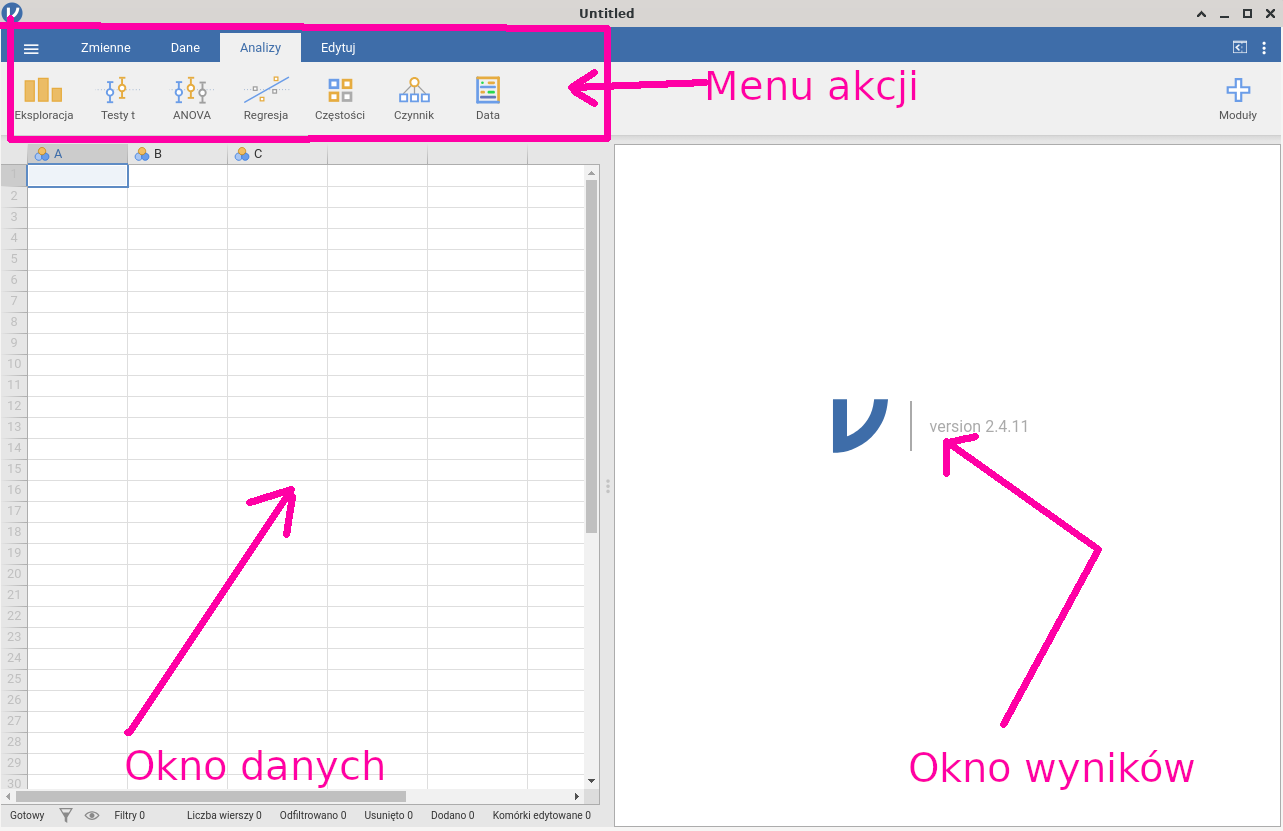
\includegraphics[width=0.95\linewidth]{./jamovi_main_screen} \caption{Ekran startowy Jamovi}\label{fig:mainscreen}
\end{figure}

Menu akcji umożliwia wykonanie podstawowych akcji:

\begin{itemize}
\item
  wczytanie danych i zapisanie danych (pierwsza pozycja menu oznaczona jako
  trzy poziome kreski);
\item
  podgląd (w sensie skontrolowania wartości zmiennych) i modyfikację
  danych (pozycje \textbf{Zmienne} oraz \textbf{Dane});
\item
  wykonanie obliczeń (pozycja \textbf{Analizy});
\item
  modyfikowanie raportu (pozycja \textbf{Edit}).
\end{itemize}

Typowa sesja w \textbf{Jamovi}:

\begin{enumerate}
\def\labelenumi{\arabic{enumi}.}
\item
  Wczytanie danych z pliku o praktycznie dowolnym formacie. Jeżeli przykładowo
  dane są wynikiem wykonania badania ankietowego z wykorzystaniem Formularzy Google to
  zalecamy posługiwanie się formatem CSV.
\item
  Transformacja danych. Przekodowanie wartości nominalnych na rangi. Przekodowanie
  wartości liczbowych na nominalne.
  Odwrócenie pytań odwróconych. Obliczenie sum/średnich rang dla wielu zmiennych.
\item
  Wykonanie obliczeń:

  \begin{enumerate}
  \def\labelenumii{\arabic{enumii}.}
  \tightlist
  \item
    Analiza struktury (\textbf{Eksploracja}).
  \item
    Analiza zależności między zmienną liczbową a nominalną (\emph{testy t}/\textbf{ANOVA}).
  \item
    Analiza zależności między zmiennymi liczbowymi: współczynnik korelacji
    liniowej/macierz korelacji (\emph{Regresja}).
  \item
    Analiza zależności między zmienną liczbową a zmiennymi liczbowymi/nominalnymi:
    regresja liniowa i logistyczna (\textbf{Regresja}).
  \item
    Analiza zależności między zmiennymi nominalnymi: tablica wielodzielcza, test
    chi-kwadrat zgodności (\emph{Częstości}).
  \end{enumerate}

  Wykonanie obliczeń jest banalnie proste i sprowadza się do wybrania myszką odpowiednich
  zmiennych oraz procedury, która ma być wykonana.
  Wynik obliczeń pojawia się natychmiast w \textbf{oknie wyników}. Jeżeli coś
  nam nie wyszło można procedurę poprawić a poprzedni wynik usunąć z okna wynikowego.
\item
  Zapisania danych (pozycja trzy poziome kreski). Po skończeniu pracy wynik można
  zapisać, żeby np. wysłać wykładowcy lub nie zaczynać od zera jeżeli będziemy musieli
  pracę kontynuować, bo wykładowca chciał żebyśmy coś poprawili.
\end{enumerate}

\hypertarget{analiza-ankiety-satysfakcja-wiedza-o-paleniu-zamiar-odejux15bcia}{%
\section{Analiza ankiety: satysfakcja -- wiedza o paleniu -- zamiar odejścia}\label{analiza-ankiety-satysfakcja-wiedza-o-paleniu-zamiar-odejux15bcia}}

Przykład nieco absurdalny, ale za to w zwartej postaci ilustrujący
praktyczne sposoby transformacji danych oraz
wykorzystania wszystkich procedur omawianych w podręczniku.

\hypertarget{wczytanie-danych}{%
\subsection{Wczytanie danych}\label{wczytanie-danych}}

W wyniku przeprowadzenia badania ankietowego zebrano za pomocą Formularza Google
dane dotyczące
satysfakcji/zamiaru odejścia oraz wiedzy nt. szkodliwości palenia tytoniu.
Wyniki wyeksportowano do arkusza kalkulacyjnego, którego początek
wygląda jak na rysunku \ref{fig:GoogleFormsTestA}:

\begin{figure}
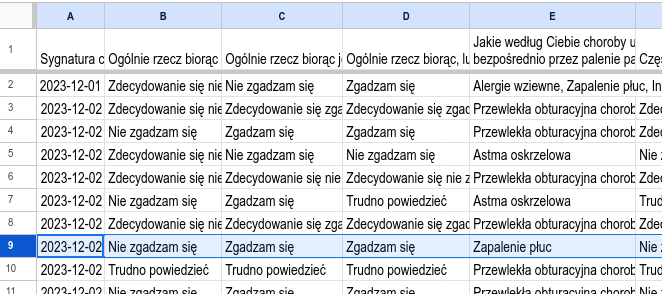
\includegraphics[width=0.95\linewidth]{./GoogleFormsTestA} \caption{Fragment przykładowej ankiety}\label{fig:GoogleFormsTestA}
\end{figure}

Ankieta składa się z 10 następujących pytań:

Ogólnie rzecz biorąc nie lubię swojej pracy (kolumna \texttt{B}),
Ogólnie rzecz biorąc jestem zadowolony ze swojej pracy (\texttt{C}),
Ogólnie rzecz biorąc, lubię tu pracować (\texttt{D}),
Jakie według Ciebie choroby układu oddechowego mogą być spowodowane
bezpośrednio przez palenie papierosów? (\texttt{E}),
Często poważnie rozważam odejście z obecnej pracy (\texttt{F}),
Zamierzam rzucić obecną pracę (\texttt{G}),
Zacząłem szukać innej pracy (\texttt{H}),
Płeć (\texttt{I}),
Wiek (w latach) (\texttt{J}),
oraz Staż pracy (\texttt{K}).

Ponadto Formularz Googla dodał automatycznie sygnaturę czasową
jako zawartość pierwszej kolumny (\texttt{A}).

Zmieniamy wartości w pierwszym wierszu, który powinien zawierać nazwy zmiennych.
Nazwy zmiennych powinny być jednowyrazowe i w miarę krótkie żeby się później
można nimi wygodnie posługiwać. Jednocześnie nie powinny być za krótkie żeby
od razu było widać jakie dane zawiera zmienna.

Jak widać
pytania z kolumn \texttt{B}--\texttt{D} mierzą to samo (satysfakcję)
więc zmieniamy im nazwę na bardziej zwartą \texttt{s1}, \texttt{s2} oraz \texttt{s3} (\texttt{s} od satysfakcja).
Podobnie
ponieważ pytania z kolumn \texttt{F}--\texttt{H} też mierzą to samo (zamiar odejścia), to
też zmieniamy nazwy na coś krótszego: \texttt{zo1}, \texttt{zo2}, \texttt{zo3}. Kolumnę \texttt{E} nazywamy
\texttt{wiedza\_nt\_palenia} a kolumny \texttt{I}, \texttt{J} oraz \texttt{K} odpowiednio:
\texttt{plec}, \texttt{wiek} oraz \texttt{staz}.

Teraz arkusz wygląda jak na rysunku \ref{fig:GoogleFormsTestHdr}.

\begin{figure}
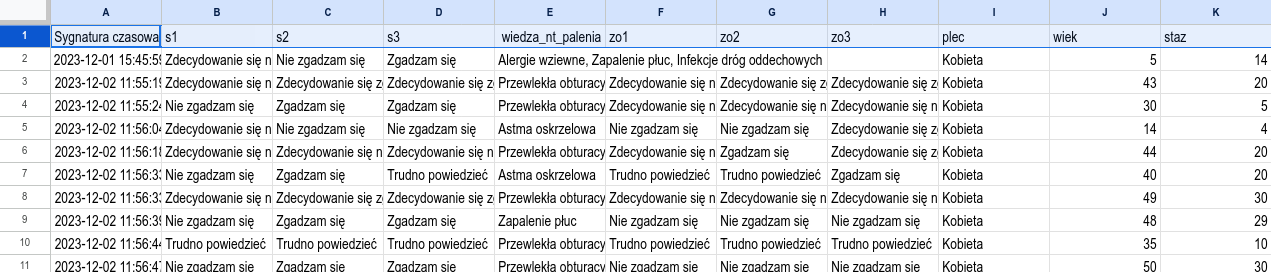
\includegraphics[width=0.95\linewidth]{./GoogleFormsTestHdr} \caption{Fragment przykładowej ankiety}\label{fig:GoogleFormsTestHdr}
\end{figure}

Arkusz eksportujemy wybierając format CSV. Bez problemu powinniśmy
go wczytać do Jamovi (trzy poziome kreski →\texttt{Otwórz}). Jeżeli import
się powiódł, to powinniśmy zobaczyć coś podobnego do tego co widać na rysunku \ref{fig:dataimport}.

Reasumując:

\begin{itemize}
\item
  Pytania oznaczone jako \texttt{s1}/\texttt{s2}/\texttt{s3} mierzą
  \textbf{satysfakcję z pracy}; pytania \texttt{zo1}/\texttt{zo2}/\texttt{zo3} mierzą \textbf{zamiar odejścia
  z pracy}. Pytania \texttt{s1}--\texttt{s3} oraz \texttt{zo1}--\texttt{zo3} są pytaniami jednokrotnego wyboru.
\item
  Pytanie oznaczone jako \texttt{wiedza\_nt\_palenia} mierzy wiedzę na temat palenia tytoniu.
  Jest to przykład wykorzystania pytania z wielokrotnym wyborem.
\item
  Pytania \texttt{plec}, \texttt{wiek}, \texttt{staz} mierzą płeć (\texttt{kobieta}/\texttt{mężczyzna}), wiek (lata ukończone)
  oraz staż pracy (lata przepracowane).
\item
  Pierwsza kolumna nie jest potrzebna, ale jest dodawana przez aplikację Formularze Google.
\end{itemize}

\begin{figure}
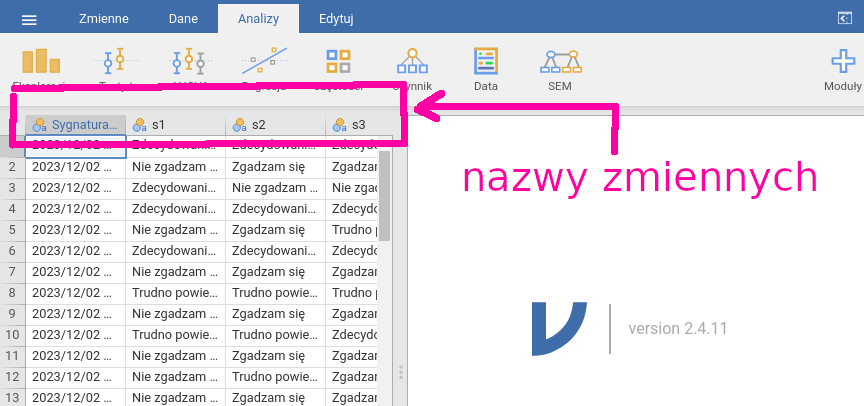
\includegraphics[width=0.95\linewidth]{./jamovi_data_import_small} \caption{Import danych}\label{fig:dataimport}
\end{figure}

\hypertarget{przekodowanie-danych}{%
\subsection{Przekodowanie danych}\label{przekodowanie-danych}}

Zwykle zawartość arkusza zawierającego wyniki ankiety wymaga przekodowania.
W naszym przykładzie należy wykonać:

\begin{itemize}
\item
  Zmienne \texttt{s1}--\texttt{s3} oraz \texttt{zo1}--\texttt{zo3} są mierzone w skali porządkowej. Wartości tych zmiennych
  chcemy zmienić (przekodować) na rangi wg schematu: \texttt{Zdecydowanie\ się\ nie\ zgadzam} = 1;
  \texttt{Nie\ zgadzam\ się} = 2; \texttt{Trudno\ powiedzieć} = 3 itd.
  Dodatkowo zauważmy że \texttt{s1} jest pytaniem odwróconym.
  W takich pytaniach należy przeliczyć rangi wg prostej formuły s1r = 6 - s1.

  \begin{itemize}
  \tightlist
  \item
    Miarą satysfakcji będzie suma rang s1r+s2+s3.
  \item
    Miarą zamiaru odejścia będzie suma rang zo1+zo2+zo3.
  \end{itemize}
\item
  Zmienna \texttt{plec} jest mierzona w skali nominalnej. Nie musimy jest przekodowywać
\item
  Wartość zmiennej \texttt{wiedza\_nt\_palenia} należy przekodować na liczbę wg schematu:
  za wybranie poprawnej odpowiedzi plus jeden punkt; za wybranie błędnej odpowiedzi
  minus jeden punkt.

  \begin{itemize}
  \tightlist
  \item
    Miarą wiedzy nt. palenia będzie suma punktów uzyskanych za odpowiedzi prawidłowe
    minus suma punktów uzyskanych za odpowiedzi nieprawidłowe.
  \end{itemize}
\end{itemize}

Uwaga: Sposób mierzenia wiedzy nt. palenia jest niepotrzebnie pokręcony; zamiast
pytania z wielokrotnym wyborem spośród 8 możliwości/wariantów prościej jest zastosować
8 pytań Tak/Nie po czym pytania poprawne zsumować
a pytania niepoprawne też dodać a wartość odjąć od sumy uzyskanej dla pytań poprawnych.
My o tym wiemy, że tak jest bez sensu ale pokazujemy jako przykład przekodowania
pytania z wielokrotnym wyborem.

\begin{itemize}
\tightlist
\item
  Wartości zmiennych \texttt{wiek} oraz \texttt{staz} są liczbami. Mogą być analizowane tak-jak-są
  (regresja/korelacja), ale można też je przekodować na wartości nominalne
  (mały-średni-duży staż) i zastosować metody z grupy zmienna-liczbowa/zmienna nominalna
  (takie jak test ANOVA czy Kruskala-Wallisa).
\end{itemize}

Przekodowanie wykonujemy wybierając \textbf{Dane} w menu głównym.

\begin{enumerate}
\def\labelenumi{\arabic{enumi}.}
\item
  Klikamy w nazwę zmienną, którą zamierzamy przekodować. Niech to będzie \texttt{s1}.
  Kolumna po kliknięciu zmieni kolor.
\item
  Wybieramy ikonę \texttt{Przekształcenie}. Wypełniamy jak na rysunku \ref{fig:przeksztalcenie0}.
\end{enumerate}

Uwaga: Jamovi nie zmieni wartości zmiennej \texttt{s1} tylko utworzy nową zmienną
z przekodowanymi wartościami. Zmienna na podstawie której jest tworzona
nowa zmienna nazywa się źródłową (\texttt{s1} w naszym przykładzie jest źródłowa).

\begin{figure}

\includegraphics[width=0.95\linewidth]{./jamovi_przeksztalcenie_0_small} \caption{Przekształcenie}\label{fig:przeksztalcenie0}
\end{figure}

Wpisujemy sensowną nazwę (na przykład \texttt{s1p} od przekodowana). Jak będziemy
używać sensownych nazwa łatwiej będzie nam się pracowało. Dobrze jest
też podać w opisie co zawiera zmienna.

Klikamy w pole wyboru na dole (obok napisu \texttt{za\ pomocą\ przekształcenia}).
Powinniśmy zobaczyć coś podobnego do tego co widać na rysunku \ref{fig:przeksztalcenie1}.

\begin{figure}
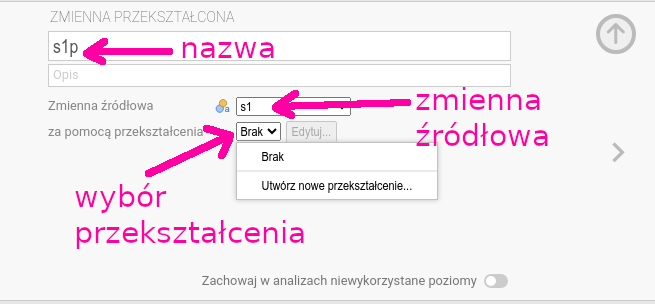
\includegraphics[width=0.95\linewidth]{./jamovi_przeksztalcenie_1} \caption{Przekształcenie}\label{fig:przeksztalcenie1}
\end{figure}

Wybieramy \texttt{Utwórz\ nowe\ przekształcenie}. Wpisujemy sensowną nazwę
przekształcenia (na przykład \texttt{Likert2R5}) oraz formułę przekształcenia:

\begin{verbatim}
IF ($source=="Zdecydowanie się nie zgadzam", 1,
 IF ($source=="Nie zgadzam się", 2,
   IF ($source=="Trudno powiedzieć", 3,
      IF ($source=="Zgadzam się", 4, 5))))
\end{verbatim}

Formuła może wydawać się przerażająca, ale jest koncepcyjnie bardzo prosta:

\begin{verbatim}
IF (warunek, jeżeli-prawda, jeżeli-fałsz)
\end{verbatim}

\texttt{Warunek} to fragment \texttt{\$source=="Zdecydowanie\ się\ nie\ zgadzam"}:

\begin{itemize}
\item
  \texttt{\$source} oznacza bieżącą wartość zmiennej źródłowej;
\item
  \texttt{==} to \textbf{operator} równości; jest więcej operatorów, które można
  wybrać z menu;
\item
  \texttt{\$source=="Zdecydowanie\ się\ nie\ zgadzam"} oznacza, że jeżeli
  bieżącą wartością w kolumnie źródłowej jest \texttt{Zdecydowanie\ się\ nie\ zgadzam}
  to wykonaj \texttt{jeżeli-prawda}; w wypadku przeciwnym wykonaj \texttt{jeżeli-fałsz}.
\end{itemize}

\texttt{jeżeli-prawda} to zwykle wstawienie nowej wartości;
\texttt{jeżeli-fałsz} to często następna formuła \texttt{IF} albo wstawienie innej
nowej wartości. Przykładowo jeżeli
bieżącą wartością w kolumnie źródłowej jest \texttt{Zdecydowanie\ się\ nie\ zgadzam}
to wstaw \texttt{1}, jeżeli nie jest to wstaw \texttt{0}:

\begin{verbatim}
  IF ($source=="Zdecydowanie się nie zgadzam", 1,0)
\end{verbatim}

Ponieważ w naszym przykładzie mamy do przekodowania nie dwie a 5 wartości
musimy użyć 4 warunków, które
są zagnieżdżone jeden w drugim. Można powyższe przepisać, można
też skopiować z podręcznika i wkleić do Jamovi (por. rys. \ref{fig:przeksztalcenie1p}).

\begin{figure}
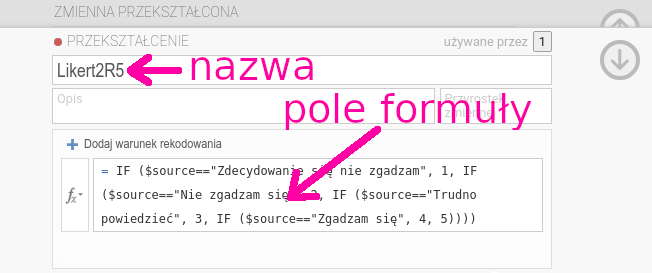
\includegraphics[width=0.95\linewidth]{./jamovi_przeksztalcenie_1p} \caption{Przekształcenie}\label{fig:przeksztalcenie1p}
\end{figure}

Naciskamy Enter i gotowe. Zostaje utworzona zmienna \texttt{s1p}
zawierająca zamiast napisów rangi.

Jeżeli uporaliśmy się z przekodowaniem \texttt{s1}
ustawiamy kursor na \texttt{s2} w okno danych. Naciskamy ikonę \texttt{Przekształcenie}.
Upewniamy się, że zmienną źródłową jest \texttt{s2}.
Zmieniamy nazwę nowej zmiennej na \texttt{s2p}. Klikamy
w pole wyboru przekształcenia. Poprzednio były tam tylko dwie pozycje
\texttt{Brak} oraz \texttt{Utwórz\ nowe\ przekształcenie} teraz jest trzecia pozycja
\texttt{Likert2R5} czyli przekształcenie, które zdefiniowaliśmy dla zmiennej \texttt{s1p}.
Wybieramy \texttt{Likert2R5} bo zmienną \texttt{s2} chcemy przekodować dokładnie
w ten sam sposób jak \texttt{s1}. Po wybraniu przekształcenia w oknie danych
pojawia się nowa zmienna \texttt{s2p} (por. rys. \ref{fig:przeksztalcenie3}).

\begin{figure}
\includegraphics[width=0.95\linewidth]{./jamovi_przeksztalcenie_3} \caption{Przekształcenie}\label{fig:przeksztalcenie3}
\end{figure}

W podobny łatwy sposób przekodowujemy \texttt{s3} oraz \texttt{zo1}, \texttt{zo2}, \texttt{zo3}.

\textbf{Uwaga}: polecenie \texttt{IF} wpisujemy używając dużych liter. Słowo
\texttt{\$source} wpisujemy tak jak jest to zademonstrowane (\texttt{\$Source} jest błędem).

Przekodowanie pytania z możliwością wielokrotnego wyboru jest równie
proste, tyle że pisania jest więcej. Zmienna \texttt{wiedza\_na\_temat\_palenia} może zawierać
do ośmiu następujących napisów oddzielonych średnikami:
\texttt{Przewlekła\ obturacyjna\ choroba\ płuc},
\texttt{Astma\ oskrzelowa},
\texttt{Alergie\ wziewne},
\texttt{Gruźlica} (B),
\texttt{Zapalenie\ płuc} (B),
\texttt{Przewlekłe\ zapalenie\ oskrzeli},
\texttt{Infekcje\ dróg\ oddechowych},
\texttt{Palenie\ nie\ powoduje\ chorób\ układu\ oddechowego} (B).

Odpowiedzi błędne oznaczono jako (B).

W arkuszu lub oknie danych Jamovi ta zmienna wygląda jakoś tak:

\begin{verbatim}
...,Przewlekła obturacyjna choroba płuc,...
...,Przewlekła obturacyjna choroba płuc;Astma oskrzelowa;...
...,Astma oskrzelowa,
...,Astma oskrzelowa;Gruźlica;Przewlekłe zapalenie oskrzeli,...
...,Przewlekła obturacyjna choroba płuc;Astma oskrzelowa;...
\end{verbatim}

Należy zsumować wystąpienia poprawne i wystąpienia błędne. W tym celu trzeba utworzyć tyle
nowych zmiennych ile jest wariantów odpowiedzi, czyli w naszym przykładzie osiem. Każda
nowa zmienna jest przekodowywana za pomocą prostej formuły wykorzystującą funkcję \texttt{CONTAINS} (zawiera).
Przykładowo pierwsza (nazwijmy ją \texttt{wiedz1p}) powinna być utworzona w oparciu o następujące przekształcenie:

\begin{verbatim}
CONTAINS("Przewlekła obturacyjna choroba płuc", $source)
\end{verbatim}

Jak to wygląda w oknie programu Jamovi przedstawiono na rysunkach \ref{fig:przeksztalcenie4}
oraz \ref{fig:przeksztalcenieContains}.

\begin{figure}
\includegraphics[width=0.95\linewidth]{./jamovi_przeksztalcenie_4} \caption{Przekształcenie}\label{fig:przeksztalcenie4}
\end{figure}

\begin{figure}
\includegraphics[width=0.95\linewidth]{./jamovi_przeksztalcenie_contains_small} \caption{Przekształcenie}\label{fig:przeksztalcenieContains}
\end{figure}

Funkcja CONTAINS wstawi 1 jeżeli \texttt{\$source} zawiera \texttt{Przewlekła\ obturacyjna\ choroba\ płuc}.
Oczywiście następna zmienna powinna zawierać \texttt{Astma\ oskrzelowa}:

\begin{verbatim}
CONTAINS("Astma oskrzelowa", $source)
\end{verbatim}

I tak dalej aż do ostatniego wariantu odpowiedzi:

\begin{verbatim}
CONTAINS('Alergie wziewne', $source)
CONTAINS('Gruźlica', $source)
CONTAINS('Zapalenie płuc', $source)
CONTAINS('Przewlekłe zapalenie oskrzeli', $source)
CONTAINS('Infekcje dróg oddechowych', $source)
CONTAINS('Palenie nie powoduje chorób układu oddechowego', $source)
\end{verbatim}

Każda zmienna \texttt{wiedza1}\ldots{}\texttt{wiedza8} zawiera 1 jeżeli ankietowany wskazał dany wariant lub zero jeżeli
nie wskazał.

Ostatnia sprawa to przekodowanie liczb na wartości nominalne. Przykładowo chcemy podzielić
ankietowanych na grupy stażowe: mały (do pięciu lat), średni (5--15 lat), duży (16 i więcej) staż pracy.

Wartości liczbowe stażu pracy zawiera zmienna \texttt{staz}. Aby ją przekodować
należy użyć następującego przekształcenia:

\begin{verbatim}
IF ($source < 5, "M",
  IF ($source < 16, "S", "D"))
\end{verbatim}

Poleceń \texttt{IF} musi być o jedno mniej niż mamy klas. W naszym przykładzie zatem dwa. Jeżeli
\texttt{staż} jest mniejszy od 5 wstawiony zostanie napis \texttt{M}, jeżeli \texttt{staż} jest mniejszy od 16
wstawiony zostanie napis \texttt{S} a w przeciwnym wypadku zostanie wstawiony napis \texttt{D}.

Gdyby ktoś się niepokoił że 3 spełnia jednocześnie \texttt{\$source\ \textless{}\ 5} oraz \texttt{\$source\ \textless{}\ 16}
to dodamy, że pierwszy się liczy. Przekształcenie kończy działanie po spełnieniu pierwszego warunku i nie
wykonuje dalszych porównań. Dlatego liczba 3 zostanie zamieniona na \texttt{M} a nie na \texttt{S}.

Podobnie przekodowujemy zmienną \texttt{wiek}.

\hypertarget{wyliczenie-nowych-zmiennych}{%
\subsection{Wyliczenie nowych zmiennych}\label{wyliczenie-nowych-zmiennych}}

\textbf{Przekodowanie} to była w zasadzie zamiana sposobu mierzenia. \textbf{Wyliczenie} to utworzenie
nowej zmiennej, zwykle w oparciu o jakąś formułę matematyczną. Na przykład odwrócenie pytanie s1p
realizuje \texttt{s1pr\ =\ 6\ -\ s1p}. Satysfakcja to suma rang z trzech pytań:
\texttt{satysfakcja\ =\ \ s1pr\ +\ s2p\ +\ s3p}.

W celu wyliczanie nowych zmiennych należy wybrać Dane Oblicz. Pojawia się okno
zmiennej wyliczonej zatytułowane \texttt{ZMIENNA\ WYLICZONA}.

Pierwszy pasek zawiera nazwę zmienną (domyślnie nazwę kolumny w konwencji arkusza kalkulacyjnego,
w przykładzie
jest to litera \texttt{H}) W polu definiowania zmiennej należy wpisać
stosowną formułę matematyczną. W przypadku odwracania pytania \texttt{s1p} będzie to:

\begin{verbatim}
6 - s1p
\end{verbatim}

W przypadku liczenia łącznej satysfakcji (por. rys. \ref{fig:zmiennaSatysfakcja}):

\begin{verbatim}
SUM(s1pr, s2p, s3p)
\end{verbatim}

\begin{figure}
\includegraphics[width=0.95\linewidth]{./jamovi_zmienna_satysfakcja} \caption{Obliczanie nowej zmiennej}\label{fig:zmiennaSatysfakcja}
\end{figure}

Oczywiście wcześniej musimy utworzyć zmienną \texttt{s1pr}, inaczej Jamovi zgłosi błąd.

Jeżeli nie chcemy sumy, ale np. średnią powinniśmy użyć:

\begin{verbatim}
MEAN(s1pr, s2p, s3p)
\end{verbatim}

Inne funkcje matematyczne są dostępne po kliknięciu w pole wyboru znajdujące się po lewej
stronie pola definiowania zmiennej.

Powiedzieliśmy, że miarą wiedzy nt. palenia będzie suma punktów uzyskanych za odpowiedzi prawidłowe minus
suma punktów uzyskanych za odpowiedzi nieprawidłowe. Odpowiedzi prawidłowe to
\texttt{w1p}, \texttt{w2p}, \texttt{w3p}, \texttt{w6p} oraz \texttt{w7p}. Odpowiedzi błędne to \texttt{w4p}, \texttt{w5p}, \texttt{w8p}. Zatem
w polu definiowania zmiennej wpisujemy:

\begin{verbatim}
SUM(w1p, w2p, w3p, w6p, w7p) - SUM(w4p, w5p, w8p)
\end{verbatim}

\hypertarget{analiza-struktury}{%
\subsection{Analiza struktury}\label{analiza-struktury}}

Wybieramy \texttt{Analizy}→\texttt{Eksploracja}→\texttt{Statystyki\ opisowe}.

W wyświetlonym oknie po lewej deklarujemy co ma być liczone. Wynik
pojawi się po prawej (por. rys. \ref{fig:statystykiOpisoweOkno}).

\begin{figure}
\includegraphics[width=0.95\linewidth]{./jamovi_statystyki_opisowe_okno} \caption{Statystyki opisowe}\label{fig:statystykiOpisoweOkno}
\end{figure}

Ustawiamy kursor na zmiennej, która nas interesuje i klikamy w strzałkę górną.
Jeżeli chcemy podzielić wartości zmiennej na grupy według jakiejś
zmiennej nominalnej, to ustawiamy kursor na tej zmiennej nominalnej
(na przykład \texttt{plec}) i klikamy strzałkę dolną.

Można analizować wiele zmiennych na raz (por. rys. \ref{fig:statystykiSpisoweWynik}).
Wystarczy w tym celu ustawić
kursor na zmiennej i kliknąć w odpowiednią strzałkę. Zawartość okna
wynikowego zostanie automagicznie uaktualniona.

\begin{figure}
\includegraphics[width=0.95\linewidth]{./jamovi_statystyki_opisowe_wynik} \caption{Statystyki opisowe}\label{fig:statystykiSpisoweWynik}
\end{figure}

Poniżej okien wyboru zmiennych są zakładki określające precyzyjnie, co ma
być obliczone oraz jakie wykresy mają zostać wyrysowane.
Przykładowo domyślny wydruk nie zawiera
rozstępu kwartylowego. Żeby go dodać do wyniku należy
w zakładce \texttt{Statystyki} zaznaczyć przycisk \texttt{IQR}.

\hypertarget{analiza-zaleux17cnoux15bci-zmienne-nominalne}{%
\subsection{Analiza zależności: zmienne nominalne}\label{analiza-zaleux17cnoux15bci-zmienne-nominalne}}

Wybieramy \texttt{Analizy}→\texttt{Częstości}→\texttt{Próby\ niezależne}.

Podobnie jak w przypadku analizy struktury jest wyświetlana
lista zmiennych oraz okna i strzałki pozwalające
wygodnie wybrać to co ma być analizowane. Jest to tak proste
że wystarczy przyjrzeć się przykładowemu rysunkowi żeby
wiedzieć jak postępować. Przykładową analizę zależności
pomiędzy zmiennymi nominalnymi \texttt{zamiarOklasa} oraz \texttt{staz.klasa} przedstawia rysunek \ref{fig:tabeleKrzyzowe}.

\begin{figure}
\includegraphics[width=0.95\linewidth]{./jamovi_tabele_krzyzowe} \caption{Tabele krzyżowe}\label{fig:tabeleKrzyzowe}
\end{figure}

\hypertarget{analiza-zaleux17cnoux15bci-zmienna-liczbowazmienna-nominalna}{%
\subsection{Analiza zależności: zmienna liczbowa/zmienna nominalna}\label{analiza-zaleux17cnoux15bci-zmienna-liczbowazmienna-nominalna}}

Jeżeli zmienna nominalna (zwana grupującą) przyjmuje dwie wartości
wybieramy \texttt{Analizy}→\texttt{Testy\ t}→\texttt{Test\ t\ dla\ prób\ niezależnych}.
Zmienne zależne to zmienne, których wartości zostaną podzielone na grupy.
Ustawiamy kursor kolejno na zmiennej, która nas interesuje i klikamy w strzałkę górną.
Ustawiamy kursor na zmiennej grupującej
(na przykład \texttt{plec}) i klikamy strzałkę dolną (por. rys. \ref{fig:testyJamovi}).

Zaznaczamy przyciski \texttt{Test\ Welcha}, \texttt{U\ Manna-Whitneya} (w sekcji \textbf{Testy}) oraz \texttt{Test\ normalności}
(w sekcji \textbf{Weryfikacja założeń})

Jeżeli zmienna nominalna więcej niż dwie wartości
wybieramy \texttt{Analizy}→\hspace{0pt}\texttt{ANOVA}→\hspace{0pt}\texttt{Jednoczynnikowa\ ANOVA}. Zmienne zależne
i grupujące wybieramy w identyczny sposób jak w przypadku testu Welcha (por. rys. \ref{fig:anovaJamovi}).
Zaznaczamy przyciski \texttt{Nie\ zakładaj\ równości\ (Test\ Welcha)} (w sekcji \textbf{Wariancje}) oraz \texttt{Test\ normalności}
(w sekcji \textbf{Weryfikacja założeń}) i \texttt{Tabela\ statystyk\ opisowych} (w sekcji \textbf{Dodatkowe statystyki}).

Jeżeli wynik testu Shapiro-Wilka wskaże, że rozkład zmiennej zależnej nie jest normalny należy
wykonać test Kruskala-Wallisa wybierając \texttt{Jednoczynnikowa\ ANOVA\ Test\ Kruskala-Wallisa}.

\begin{figure}
\includegraphics[width=0.95\linewidth]{./jamovi_testy_welch} \caption{Test dla prób niezależnych}\label{fig:testyJamovi}
\end{figure}

\begin{figure}
\includegraphics[width=0.95\linewidth]{./jamovi_anova} \caption{Jednoczynnikowa ANOVA}\label{fig:anovaJamovi}
\end{figure}

\hypertarget{analiza-zaleux17cnoux15bci-zmienna-liczbowazmienna-liczbowa-lub-nominalna}{%
\subsection{Analiza zależności: zmienna liczbowa/zmienna liczbowa lub nominalna}\label{analiza-zaleux17cnoux15bci-zmienna-liczbowazmienna-liczbowa-lub-nominalna}}

Wybieramy \texttt{Analizy}→\texttt{Regresja}→\texttt{Regresja\ liniowa}.

Interfejs jest podobny do poprzednio opisywanych. Wybieramy
zmienną zależną (musi oczywiście być liczbowa) klikając w górną strzałkę.
Zmienne niezależne mierzone w skali liczbowej
klikając w środkową strzałkę. Zmienne niezależne mierzone
w skali nominalnej klikając w dolną strzałkę.
Wynik automagicznie pojawia się w lewym oknie (por. rys. \ref{fig:regresjaLiniowa}).

\begin{figure}
\includegraphics[width=0.95\linewidth]{./jamovi_regresja_liniowa} \caption{Regresja liniowa}\label{fig:regresjaLiniowa}
\end{figure}

\hypertarget{regresja-logistyczna}{%
\subsection{Regresja logistyczna}\label{regresja-logistyczna}}

Wybieramy \texttt{Analizy}→\texttt{Regresja}→\texttt{Regresja\ logistyczna}→\texttt{Dwie\ wartości}.

Interfejs jest łudząco podobny do analizy regresji. Wybieramy
zmienną zależną klikając w górną strzałkę. Zmienna ta
\textbf{musi} być zmienną dwuwartościową.

Zmienne niezależne mierzone w skali liczbowej
wybieramy klikając w środkową strzałkę, a zmienne niezależne mierzone
w skali nominalnej klikając w dolną strzałkę.

\hypertarget{redagowanie-raportu}{%
\subsection{Redagowanie raportu}\label{redagowanie-raportu}}

Zwykle dobrze jest dodać jakieś dodatkowe objaśnienia do wyników
obliczeń wygenerowanych
przez program i Jamovi nam to umożliwia.
Wybierając \texttt{Edytuj} przechodzimy do prostego edytora umożliwiającego redagowanie raportu
w oknie wyników a obsługa tego menu jest tak banalnie prosta, że nie wymaga
jakiś specjalnych objaśnień.

\hypertarget{literatura}{%
\chapter*{Literatura}\label{literatura}}
\addcontentsline{toc}{chapter}{Literatura}

Beaglehole, Robert, Ruth Bonita, and Tord Kjellstrom. 1996. \emph{Podstawy Epidemiologii}. Instytut Medycyny Pracy.

Bland, Martin. 2015. \emph{An Introduction to Medical Statistics}. Oxford University Press.

Machin, David, Michael J Campbell, and Stephen J Walters. 2007. \emph{Medical Statistics}. John Wiley.

\end{document}
